\documentclass[article,type=msc,colorback,accentcolor=tud9c]{tudthesis}

% usepackages
% =============================================================
\usepackage[utf8]{inputenc}
\usepackage[russian,english]{babel}

% font
\usepackage{bm}
\usepackage{pifont}
\usepackage{mxedruli}
\usepackage{soul}

% tables
\usepackage{array}
\usepackage{colortbl}
\usepackage{tabularx}
\usepackage{multirow}
\usepackage{booktabs}

\usepackage{adjustbox} 		% rotation of content

% plotting
\usepackage{tikz}
\usepackage{pgfplots}

% boxes
\usepackage[many]{tcolorbox}

% misc
\usepackage[absolute,overlay]{textpos}

% template
% =============================================================

\setbeamertemplate{section in toc}[square]

% some simple commands
% =============================================================

\newcommand{\highlight}[1]{\textcolor{tud1a}{\textbf{#1}}}

\newcommand{\gr}{\cellcolor{lightgray}}

\newcolumntype{?}{!{\vrule width 1.5pt}}

% absolute positioning of images
\newcommand{\abspos}[4]{
	\begin{textblock}{100}(#1,#2)
		\textblockcolour{white}
      		\includegraphics[scale=#4]{#3}
    	\end{textblock}
}

% divide into left and right content
\newcommand{\divideTwo}[4]{
	\begin{minipage}{#1\textwidth}
		#2
	\end{minipage}
	\hfill
	\begin{minipage}{#3\textwidth}
		#4
	\end{minipage}
}

% probing task template
\newcommand{\probingtask}[5]{
	\footnotesize
	\begin{itemize}\setlength\itemsep{1em}
		\item \textbf{Category:} \\ #1
		\item \textbf{Description:} \\ #2
		\item \textbf{Implementation:} \\ #3
		\item \textbf{Languages:} #4
		\item \textbf{Example:} \\ #5
	\end{itemize}
}

% language template
\newcommand{\lang}[5]{
	EN 	\ifnum#1=51\textcolor{green}{\ding{51}}\else\textcolor{red}{\ding{55}}\fi~~~~
	DE 	\ifnum#2=51\textcolor{green}{\ding{51}}\else\textcolor{red}{\ding{55}}\fi~~~~
	RU 	\ifnum#3=51\textcolor{green}{\ding{51}}\else\textcolor{red}{\ding{55}}\fi~~~~
	TR 	\ifnum#4=51\textcolor{green}{\ding{51}}\else\textcolor{red}{\ding{55}}\fi~~~~
	KA 	\ifnum#5=51\textcolor{green}{\ding{51}}\else\textcolor{red}{\ding{55}}\fi
}

% rotated cell content
\newcolumntype{R}[2]{%
    >{\adjustbox{angle=#1,lap=\width-(#2)}\bgroup}%
    l%
    <{\egroup}%
}
\newcommand*\rot{\multicolumn{1}{R{90}{1em}}}
\newcommand*\rotff{\multicolumn{1}{R{45}{1em}}}

% red star
\newcommand{\rs}{\textcolor{red}{\textbf{*}}}

% divider page
\newcommand{\divider}[1]{
	{\begin{frame}[plain]
		\vfill\centering
		\begin{tcolorbox}[width=4in,interior hidden,boxsep=5pt,left=0pt,right=0pt,top=2mm,
			bottom=2mm,sharp corners,colback=tud1a!40,colframe=tud1a]%%
			\centering
			\textbf{Section:} \\
			\Large \textbf{#1}
		\end{tcolorbox}
		\vfill
		\centering
		
\includegraphics[scale=0.8]{tud_logo}
		\vfill
	\end{frame}}
}

% text align
\newcommand\textalign[2][]{%
	\ifx#1l\relax
  		\makebox[0pt][l]{#2}%
	\else
  		\ifx#1r\relax
    			\makebox[0pt][r]{#2}%
  		\else  
    			\ifx#1c\relax
      				\makebox[0pt][c]{#2}%
    	\fi\fi\fi
}

% centered X column
\newcolumntype{Y}{>{\centering\arraybackslash}X}


% BEGIN OF DOCUMENT
% ==========================================
\begin{document}

% title of the thesis
\thesistitle{Interpretability of Sentence Embeddings in low-resource Languages}{}
% name of author
\author{Daniel Wehner}
% birhtplace of author
\birthplace{Bad Kissingen}
% referees
\referee{Dr. Steffen Eger}{Dr. Johannes Daxenberger}
% department
\department{Fachbereich Informatik}
% group
\group{Ubiquitous Knowledge Processing}
% date of the exam
\dateofexam{\today}{\today}
% tu prints
%\tuprints{12345}{1234}

% make the thesis title
\makethesistitle

% name under signature
\affidavit{Daniel Wehner}

\pagenumbering{roman}

\section*{Abstract}
Sentence embeddings have become ubiquitous in the field of Natural Language Processing (NLP). Despite the incredible variety of sentence embedding algorithms, it is still not entirely clear what aspects of sentences are captured by such representations. However, an enormous amount of research has already been conducted on the evaluation of sentence embeddings in the English language. Unfortunately, languages different from English are considered less frequently; and if they are taken into account, the multi-lingual setting is often restricted to higher-resource languages like German, French or Spanish. Languages for which significantly less resources are available are on the other hand investigated only rarely. This circumstance motivates to put such low-resource languages more in focus and to analyze whether the results reported for English are in general transferable to these languages as well or whether the results turn out to be entirely different. This work adopts the methodology of \textit{probing tasks} popularized by \citep{Conneau.2018a} and extends this concept to a multi-lingual setting including the following five languages: English, German, Russian, Turkish and Georgian. In this work, seven probing tasks are implemented for Georgian and nine for the remaining four languages. Additionally, the embeddings are evaluated on a set of three \textit{downstream applications}. The results in these two task types are subsequently correlated in order to provide further insight into how predictive probing tasks are for downstream task performance. The correlations turn out to be language-dependent. Results for low-resource languages differ substantially from the ones obtained for English.

The fact that the evaluation setting in the context of this work partially produced results which did not comply with the literature motivated an additional stability analysis. The outcome of this experiment suggests that the usage of large and balanced data sets produces results which are more comparable with the literature. The evaluation on data sets comprising at least 30k instances is recommended since the ordering of the embeddings becomes more stable as a consequence of more training data. The effect of hyper-parameter tuning on the other hand was found to be less significant, but usually has positive effects. The evaluation in the context of this thesis is mostly done on data sets comprising 10k instances which are partially imbalanced. Therefore, the results have to be treated with caution. It is advisable that future work in this domain incorporates the recommendations given above.
\section*{Kurzfassung}
Längst haben Sentence Embeddings im Forschungsgebiet des Natural Language Processings (NLP) Einzug gehalten. Trotz der überwältigenden Vielzahl an Algorithmen in diesem Bereich ist erstaunlich wenig darüber bekannt, welche Aspekte von Sätzen durch solche Embeddings repräsentiert werden. In den vergangenen Jahren flossen einige Anstrengungen in die Evaluierung vektorieller Repräsentationen von Sätzen, dies jedoch meist ausschließlich für die Englische Sprache. Leider werden andere Sprachen nur selten betrachtet und dann vor allem solche, für die ausreichend Ressourcen zur Verfügung stehen. Beispiele hierfür sind Deutsch, Französisch oder Spanisch. Sprachen, für die derartig viele Ressourcen nicht vorhanden sind, werden zumeist vernachlässigt. Dieser Umstand motiviert dazu, solche Sprachen verstärkt in den Fokus der Forschung zu rücken. Analysen können Aufschluss darüber geben, ob Muster, die für die Englische Sprache entdeckt wurden, auch für andere Sprachen gelten, oder, ob sich die Ergebnisse gänzlich anders darbieten. Die vorliegende Arbeit bedient sich des Konzepts sogenannter \textit{Probing Tasks}, deren Benutzung vor allem von \citep{Conneau.2018a} vorangetrieben wurde. In diesem Zusammenhang wird diese Form der Evaluierung auf mehrere Sprachen erweitert: Englisch, Deutsch, Russisch, Türkisch und Georgisch. Hierbei werden sieben solcher Klassifikationsprobleme für Georgisch implementiert und neun für die restlichen vier Sprachen. Zusätzlich hierzu werden die Embeddings auf drei sogenannten \textit{Downstream Applikationen} getestet. Die Ergebnisse in diesen beiden verschiedenartigen Aufgabentypen werden nachfolgend korreliert. Die Korrelationsanalyse deckt auf, inwiefern sich das Abschneiden von Embeddings in Downstream Applikationen anhand der Ergebnisse auf den Probing Tasks vorhersagen lässt. Wie sich herausstellt, sind die Korrelationen sprachabhängig, wobei die Ergebnisse in anderen Sprachen teils stark von denen in Englisch abweichen.

Der Aufbau der Experimente im Rahmen dieser Arbeit erzeugte Ergebnisse, die zum Teil nicht mit denen aus der Literatur übereinstimmen. Dies gab Anlass dazu, eine zusätzliche Stabilitätsanalyse durchzuführen. Die Ergebnisse dieser Analyse legen nahe, dass die Benutzung großer und balancierter Datensätze von Vorteil ist. Für die Evaluierung wird deshalb empfohlen, Datensätze zu verwenden, die über mindestens 30k Instanzen verfügen, da die Rangfolge der Embeddings bei Datensätzen dieser Größenordnung deutlich stabiler wird. Der Effekt der Optimierung von Hyperparametern kann demgegenüber als vernachlässigbar eingestuft werden, nichtsdestotrotz ist für gewöhnlich ein leicht positiver Einfluss erkennbar. Die Evaluierung im Rahmen dieser Arbeit wird hauptsächlich auf Datensätzen der Größe 10k durchgeführt, die darüber hinaus teils unbalanciert sind. Aus diesem Grund haben die Ergebnisse dieser Arbeit vorläufigen Charakter und sollten weiter validiert werden. Für zukünftige Forschung in diesem Gebiet ist es daher ratsam, die oben gegebenen Empfehlungen zu berücksichtigen.
\newpage

% glossary
% Acronym definitions

\newacronym{amt}{AMT}{Amazon Mechanical Turk}
\newacronym{api}{API}{Application Programming Interface}
\newacronym{bert}{BERT}{Bidirectional Encoder Representations from Transformers}
\newacronym[plural=BiLSTMs,firstplural=Bidirectional Long Short-Term Memories (BiLSTMs)]{bilstm}{BiLSTM}{Bidirectional Long Short-Term Memory}
\newacronym{borep}{BOREP}{Bag of random Embedding Projections}
\newacronym{bov}{BOV}{Bag of Vectors}
\newacronym{bow}{BOW}{Bag of Words}
\newacronym{bpe}{BPE}{Byte Pair Encoding}
\newacronym{cbow}{CBOW}{Continuous Bag of Words}
\newacronym[plural=CNNs,firstplural=Convolutional Neural Networks (CNNs)]{cnn}{CNN}{Convolutional Neural Network}
\newacronym{cr}{CR}{Consumer/Customer Reviews}
\newacronym{csv}{CSV}{Comma Separated Value}
\newacronym{dsgvo}{DSGVO}{Datenschutz-Grundverordnung}
\newacronym{dst}{DST}{Dialogue State Tracking}
\newacronym{elmo}{ELMo}{Embeddings from Language Models}
\newacronym[plural=ESNs,firstplural=Echo State Networks (ESNs)]{esn}{ESN}{Echo State Network}
\newacronym{gdpr}{GDPR}{General Data Protection Regulation}
\newacronym{gem}{GEM}{Geometric Embeddings}
\newacronym{gnc}{GNC}{Georgian National Corpus}
\newacronym{gpu}{GPU}{Graphics Processing Unit}
\newacronym[plural=GRUs,firstplural=Gated Recurrent Units (GRUs)]{gru}{GRU}{Gated Recurrent Unit}
\newacronym{laser}{LASER}{Language-Agnostic Sentence Representations}
\newacronym{lbfgs}{LBFGS}{Limited-Memory Broyden-Fletcher–Goldfarb-Shanno}
\newacronym[plural=LSTMs,firstplural=Long Short-Term Memories (LSTMs)]{lstm}{LSTM}{Long Short-Term Memory}
\newacronym{mlm}{MLM}{Masked Language Model}
\newacronym{mlp}{MLP}{Multi-Layer Perceptron}
\newacronym{mpqa}{MPQA}{Multi-Perspective Question Answering}
\newacronym{mr}{MR}{Movie Reviews}
\newacronym{mt}{MT}{Machine Translation}
\newacronym{ner}{NER}{Named Entity Recognition}
\newacronym{nlg}{NLG}{Natural Language Generation}
\newacronym{nli}{NLI}{Natural Language Inference}
\newacronym{nlp}{NLP}{Natural Language Processing}
\newacronym{nltk}{NLTK}{Natural Language Toolkit}
\newacronym{nmt}{NMT}{Neural machine translation}
\newacronym{oov}{OOV}{Out of Vocabulary}
\newacronym{pca}{PCA}{Principal Component Analysis}
\newacronym{pos}{PoS}{Part-of-Speech}
\newacronym{ppdb}{PPDB}{Paraphrase Database}
\newacronym{relu}{ReLU}{Rectified Linear Unit}
\newacronym[plural=RNNs,firstplural=Recurrent Neural Networks (RNNs)]{rnn}{RNN}{Recurrent Neural Network}
\newacronym{rte}{RTE}{Recognizing Textual Entailment}
\newacronym{sbert}{SBERT}{Sentence BERT}
\newacronym{sif}{SIF}{Smooth Inverse Frequency}
\newacronym{snli}{SNLI}{Stanford Natural Language Inference}
\newacronym{somo}{SOMO}{Semantic Odd Man Out}
\newacronym{svd}{SVD}{Singular Value Decomposition}
\newacronym[plural=SWEMs,firstplural=Simple Word Embedding based Models (SWEMs)]{swem}{SWEM}{Simple Word Embedding based Model}
\newacronym[plural=SVMs,firstplural=Support Vector Machines (SVMs)]{svm}{SVM}{Support Vector Machine}
\newacronym{tpu}{TPU}{Tensor Processing Unit}
\newacronym{trec}{TREC}{Text Retrieval Conference}
\newacronym{ud}{UD}{Universal Dependencies}
\newacronym{ukp}{UKP}{Ubiquitous Knowledge Processing}
\newacronym{use}{USE}{Universal Sentence Embedding}
\newacronym{xml}{XML}{Extensible Markup Language}
\setlength\LTleft{0pt}
\setlength\LTright{0pt}
%\setlength\glsdescwidth{2.5\hsize}
{\renewcommand*{\arraystretch}{1.7}
	\printglossaries
}
\newpage

% symbols
\section*{Symbols}
\begin{tabbing}
	\hspace*{2mm}\=\hspace*{2.15cm}\=\kill
	\> $\mathcal{B}$				\>	data batch									\\[3mm]
	\> $c$						\>	index of center word into cocabulary $\mathcal{V}$	\\[3mm]
	\> $d$ 						\>	number of (embedding) dimensions				\\[3mm]
	\> $\mathcal{D}$				\>	data set									\\[3mm]
	\> $\mathfrak{D}$				\>	downstream task							\\[3mm]
	\> $\bm{E}$					\> 	word embedding matrix						\\[3mm]
	\> $\mathbb{E}$				\>	embedding space							\\[3mm]
	\> $\bm{h}$					\>	encoder output								\\[3mm]
	\> $\mathcal{J}(\bm{\theta})$		\>	loss function								\\[3mm]
	\> $m$						\>	window size								\\[3mm]
	\> $o$						\>	index of context word into vocabulary $\mathcal{V}$	\\[3mm]
	\> $\mathfrak{P}$				\>	probing task								\\[3mm]
	\> $\mathbb{R}$				\>	set of real numbers							\\[3mm]
	\> $r_p$						\>	Pearson correlation coefficient					\\[3mm]
	\> $r_s$						\>	Spearman correlation coefficient					\\[3mm]
	\> $rank(\bullet)$				\>	rank of a number $\bullet$ in a list of numbers		\\[3mm]
	\> $s_i$ 						\> 	$i$-th sentence of corpus						\\[3mm]
	\> $\bm{S}$					\>	embedding matrix of a sentence					\\[3mm]
	\> $T$						\>	length of a sentence / number of words in the corpus	\\[3mm]
	\> $\bm{v}_s$					\>	sentence embedding							\\[3mm]
	\> $\bm{v}_w$					\>	word embedding							\\[3mm]
	\> $\widehat{\bm{v}}$			\>	one-hot vector								\\[3mm]
	\> $\mathcal{V}$				\>	set of (unique) vocabulary words					\\[3mm]
	\> $\delta_{ant}$				\>	hyper-parameter of \textit{Attract-Repel} (antonymy)	\\[3mm]
	\> $\delta_{syn}$				\>	hyper-parameter of \textit{Attract-Repel} (synonymy)	\\[3mm]
	\> $\bm{\theta}$				\> 	learnable parameters	of a machine learning model	\\[3mm]
	\> $\tau$						\>	hinge loss									\\[3mm]
	\> $\bullet^{\intercal}$			\>	transpose of a vector or a matrix 				\\[3mm]
	\> $\oplus$ / [$\bullet, \bullet$]		\>	concatenation operator						\\[3mm]
	\> $\odot$						\>	Hadamard/point-wise product					\\[3mm]
	\> $\Vert \bullet \Vert$			\>	norm of a vector								\\	
\end{tabbing}
\newpage

% table of contents
\tableofcontents
\newpage

\setcounter{table}{0}

% list of figures / list of tables
\addtocontents{lof}{\linespread{1.7}\selectfont}
\listoffigures
\newpage
\addtocontents{lot}{\linespread{1.7}\selectfont}
\listoftables
\newpage

\pagenumbering{arabic}

% Sections
% ------------------------------------------------------------------------------------

% =======================
% Chapter: Introduction
%
% Author: Daniel Wehner
%

% -----------------------------------------------------------------------------------------------------------------------------------------------------
% Introduction
\section{Introduction}
\label{sec:introduction}

Current research in artificial intelligence increasingly focuses on better interpretability of machine learning models. Recently ratified laws such as the European \textbf{\gls{gdpr}}\footnote{The regulation is called `\gls{dsgvo}' in German.} dictate that all decisions automatically made by computers have to be justified, i.\,e. manufacturers who employ machine learning systems must be able to give reasons for why certain decision were taken.\footnote{Cf. \url{https://medium.com/pachyderm-data/hold-your-machine-learning-and-ai-models-accountable-de887177174c} \\ (retrieved: October 07, 2019)} This poses a challenging problem, since many algorithms in machine learning are so-called \textbf{`black-box' models}. Such a model is usually complicated in such a manner that it is impossible to analyze all the effects that parameters and variables inside the model have on each other.\footnote{Cf. \url{https://towardsdatascience.com/the-black-box-metaphor-in-machine-learning-4e57a3a1d2b0} \\ (retrieved: October 07, 2019)} The most prominent example of such a black-box model is the neural network algorithm which is capable of successfully dealing with vast amounts of data. The fact that neural architectures are gradually replacing classical methods which were often more interpretable exacerbates the problem even further. In the domain of \gls{nlp}, workshops like \textbf{`black-box \gls{nlp}'}\footnote{Cf. \url{https://blackboxnlp.github.io/} (retrieved: September 04, 2019)} attempt to shed light onto this (`open the black box')\footnote{Image source: \url{https://blog.f1000.com/wp-content/uploads/2017/06/black_box_blog.png} (retrieved: September 04, 2019)} and to provide explanations.

% Figure: black box
\begin{wrapfigure}{l}{0.28\textwidth}
  	\begin{center}
    		
\includegraphics[scale=0.3]{images/black_box}
		\caption[Opening the black box to improve interpretability]{Workshops like black-box \gls{nlp} try to open the black box and improve the
			interpretability of neural networks.}
  	\end{center}
\end{wrapfigure}

Understanding and explaining the output of machine learning models necessitates that the input to these models is understood as well. One of the reasons for bad training or testing performance is the quality of the input features. If the features chosen for the task to be solved are not suitable or not indicative of the class label, even the best model architecture is useless. When it comes to designing machine learning systems involving natural language input, one quickly encounters a concept called \textbf{language embeddings}. An embedding is a vectorial representation of natural language in a given granularity, be it single words, sentences, paragraphs or entire documents. Sentence embeddings are vital in \gls{nlp} because textual input cannot be dealt with by most machine learning algorithms. Despite the fruitful usage of sentence embeddings in a wide range of applications, recent research has brought to light that it is not at all clear what linguistic aspects of sentences are captured by these encodings \citep[inter alia]{Conneau.2018a}. But exactly this knowledge is invaluable when choosing the right encoder architecture for a specific task at hand. Each task is different and requires that other facets of sentences be represented in order to obtain useful predictions. Very often, \textbf{probing} as well as \textbf{downstream tasks} are used to assess the representational power of sentence embedding architectures \citep[inter alia]{Conneau.2018b}. This approach is also adopted in this thesis.

% research questions
\highlight{Research Questions.} Most of the research with respect to the evaluation of sentence embeddings is restricted to the English language.  \textbf{This thesis therefore aims to extend the focus to a multi-lingual setting by also considering lower-resource languages.} For this purpose, the languages \textbf{Russian}, \textbf{Turkish} and \textbf{Georgian} were chosen. We also conduct the analysis for \textbf{English} and \textbf{German} to compare the results to higher-resource languages as well as to the literature. \textit{This work is centered around the following research questions:} \ding{182} One of the major goals is to provide an analysis which addresses the question in how far the language chosen influences the performance of state-of-the-art sentence embedding techniques. Embeddings working well in English may not do so in other languages. \ding{183} A review of the literature further reveals that the task settings to evaluate the embeddings are not standardized and as a consequence differ from publication to publication. This is why a stability analysis is performed by varying the following factors: \texttt{language}, data set \texttt{size}, \texttt{classifier} architecture, \texttt{class balance} and \texttt{hyper-parameter optimization}. This way it is possible to draw conclusions about the stability of the relative embedding ordering.

% contributions
\highlight{Contributions.} In a first step, this document provides an overview of currently used state-of-the-art embedding algorithms. The encoders were selected such that a wide range of different techniques is included in the analysis. Most of the time pre-trained models are available only for English, i.\,e. that models have to be trained from scratch for the other languages. We trained \textit{sent2vec}, \textit{Quick-Thought} and \textit{InferSent} sentence embeddings as well as \textit{word2vec} word embeddings which form the basis for some of the sentence embedding techniques. To conduct the evaluation, it was furthermore required to setup probing and downstream tasks for each target language. For this purpose, we searched special tree banks and other corpora. In order to overcome the lack of data, especially for Georgian, it was necessary to translate some of the existing English corpora or to create new data sets from scratch. Our evaluation comprises probing as well as downstream tasks. We present the results on these two task types and successively compute correlations between them. Based on the results of the stability analysis, recommendations are given for future work and research. The following list summarizes the main contributions of this thesis in a chronological order and also serves as the guiding line for the entire project:

% enumeration of contributions
\begin{enumerate}[label=\color{tud9c}\textbf{\theenumi.}]
	\item \textbf{Review} of modern word and sentence embedding algorithms.
	\item \textbf{Acquisition of word and sentence embedding models} for the five languages English, German, Russian,
		Turkish and Georgian, either by downloading pre-trained models or by training the models from scratch
			(namely \textit{word2vec}, \textit{sent2vec}, \textit{Quick-Thought} and \textit{InferSent}).
	\item \textbf{Creation of a set of probing tasks} guided by an analysis of the characteristics of each language
		(not all probing tasks make sense in all languages, e.\,g. testing for gender information in Turkish is not
		sensible, since this concept is not present in this language).
	\item \textbf{Creation of downstream task data sets}, e.\,g. an annotated sentiment data set for the Georgian language 
		based on data extracted from Georgian Twitter.
	\item \textbf{Translation} of downstream task data sets and other corpora, e.\,g.:
	\vspace*{-2mm}
	\begin{itemize}\setlength\itemsep{-1em}
		\item \gls{snli} corpus (partially translated due to server-side constraints)
		\item \gls{ukp} sentential argument mining corpus
		\item \caps{TREC} question type data set
	\end{itemize}
	\item \textbf{Evaluation of sentence embeddings} in all five languages followed by a discussion of the results.
		A \textbf{stability analysis} is furthermore performed for a selected probing task with respect to the factors:
	\vspace*{-2mm}
	\begin{itemize}\setlength\itemsep{-1em}
		\item \texttt{Language}
		\item Data set \texttt{size}
		\item \texttt{Classifier} architecture
		\item \texttt{Class balance}
		\item \texttt{Hyper-parameter optimization}
	\end{itemize}
	\item \textbf{Recommendations} for future work and research.
\end{enumerate}

\highlight{Organization of the thesis.} This thesis is organized as follows: Chapter \vref{sec:rel_work} first of all introduces related work which represents the foundation of this thesis. The following chapter \vref{sec:word_embs} introduces the concept of word embeddings which is essential for many sentence-level algorithms. Three of the most common techniques in this domain are presented which are also used in the context of this work: \textit{word2vec}, \textit{FastText} and \textit{Attract-Repel}. Subsequently, chapter \vref{sec:sent_embs} introduces the major sentence embedding approaches used in modern applications. All of the presented embeddings are subject to the evaluations conducted at a later stage of the present thesis.

After that, chapter \vref{sec:probing_tasks} provides detailed information about the probing tasks: The chapter begins by introducing probing tasks which were already used in the literature. Subsequently, the low-resource target languages are briefly outlined in order to enable a proper assessment of the implementability of the probing tasks in these languages. These explanations are followed by details about the selection of probing tasks and how the data sets were created. Finally, the classifier architecture employed in the probing task setup is presented. Analogously, chapter \vref{sec:downstream_applications} gives information about the set of downstream applications taken into account. The evaluation results, the discussion as well as the recommendations for future work can be found in chapter \vref{sec:results_eval}, before the final chapter \vref{sec:conclusion} summarizes the main results and concludes this document.
\newpage
% =======================
% Chapter: Related Work
%
% Author: Daniel Wehner
%

% -----------------------------------------------------------------------------------------------------------------------------------------------------
% Related Work
\section{Related Work}
\label{sec:rel_work}

\vspace*{-1mm}
% -----------------------------------------------------------------------------------------------------------------------------------------------------
% Chapter Introduction
\subsection{Introduction}
\label{sec:rel_work_intro}

This chapter introduces scientific research which forms the basis for this thesis. Section \vref{sec:rel_work_embeddings} first of all demonstrates which efforts have already been devoted into the creation of monolingual and multilingual word and sentence embedding algorithms. The focus of the subsequent section \vref{sec:rel_work_eval} is on relevant literature involving the evaluation of sentence embeddings. Overall, this chapter is designed to give a general overview of all relevant concepts without explaining them in-depth. If necessary, a more detailed explanation is given in the respective chapters where the concepts are needed.

% -----------------------------------------------------------------------------------------------------------------------------------------------------
% Vectorial Representations of natural Language
\subsection{Vectorial Representations of natural Language}
\label{sec:rel_work_embeddings}

\highlight{Word embeddings.} State-of-the-art \gls{nlp} applications rely on vectorial language representations usually generated by neural networks. The idea to learn representations of natural language -- commonly known as \textbf{embeddings} -- by leveraging such neural architectures is by no means novel. One of the first approaches dates back to the year 2003 when \citep{Bengio.2003} introduced the neural language model which was devised to mitigate the \textbf{curse of dimensionality} when learning the joint probability function of word sequences. This could be achieved \textit{`by learning a \textbf{distributed representation for words}'}. The major breakthrough, however, was achieved approximately ten years later. Back then, \citep{Mikolov.2013a} proposed the famous \textit{word2vec} algorithm which comes in its two well-known flavors, \textit{Skip-Gram} and \textit{\gls{cbow}}. Only one year later, \citep{Le.2014} published another paper containing several extensions to the \textit{Skip-Gram} model. Two methods, namely \textbf{negative sampling} and \textbf{sub-sampling of frequent words} were developed to increase the robustness of the resulting word embeddings.

In the following years, many were to join this line of research and new approaches to embedding natural language were invented. Among them is a word  embedding called \textit{GloVe} proposed by \citep{Pennington.2014}. In contrast to \textit{word2vec}, this algorithm also takes \textbf{global corpus statistics} into account to improve the representations learned. Another example is \textit{FastText}, an algorithm which includes \textbf{sub-word information} by averaging character $n$-grams \citep{Bojanowski.2017}. This model is perfectly suited to handle \gls{oov} words. \citep{Mrksic.2017} further propose to fine-tune word embeddings by leveraging \textbf{linguistic constraints} like synonymy/antonymy relationships. This idea gives rise to an algorithm called \textit{Attract-Repel}. More recently, \textbf{contextualized word embeddings} have emerged. Examples include \textit{\gls{bert}} \citep{Devlin.2018} which builds on the transformer architecture \citep{Vaswani.2017} and \textit{\gls{elmo}} \citep{Peters.2018}. Such embeddings assign word representations based on the surrounding words. This way it is possible to model \textbf{polysemous words}, i.\,e. words that can have different meanings in different contexts.

\highlight{Sentence embeddings.} Soon the question arose whether it is feasible to embed even larger spans of text that go beyond single words. The notion of sentence embeddings was born. \citep{Yang.2018} differentiate between \textbf{non-parametric} and \textbf{parametric} algorithms, where techniques of the first kind (a.\,k.\,a. compositional models) are quite frequently applied and often serve as a baseline for more elaborate ones. In this context, each word in the sentence is represented by a word embedding produced by a freely-selectable word embedding algorithm which maps words to vectors. These word embeddings subsequently undergo a pooling procedure to obtain a single sentence representation. Many different pooling strategies have already been investigated in the literature: These range from average-, min-, or max-pooling to more sophisticated strategies like \textit{hierarchical pooling}. \citep{Shen.2018} named these kind of pooling algorithms \textit{\glspl{swem}}. Further, \citep{Rueckle.2018} suggest to concatenate various power means to improve the expressiveness of sentence embeddings. Other approaches like \textit{\gls{sif}} \citep{Arora.2017} or \textit{\gls{gem}} \citep{Yang.2018} make use of a method called \gls{svd}/\gls{pca} to remove projections on principal components before averaging.

Parametric methods, on the other hand, \textbf{train sentence embeddings from scratch}. One of the examples can be regarded as a generalization of the \textit{Skip-Gram} model to the sentence level. Its inventors called the algorithm \textit{Skip-Thought} \citep{Kiros.2015}. \citep{Logeswaran.2018} reformulate \textit{Skip-Thought}'s objective as a multi-class prediction problem to address several issues of the original model. Other algorithms include \textit{InferSent} \citep{Conneau.2017} which is trained on the \textit{\gls{snli}} data set \citep{Bowman.2015} and \textit{sent2vec} \citep{Pagliardini.2018} which computes sentence embeddings by averaging character $n$-grams like \textit{FastText}, but on sentence level. Recently, \citep{Reimers.2019} have introduced \	\textit{\gls{sbert}}, a version of \gls{bert} which is designed to create sentence embeddings.

\highlight{Multi-lingual embeddings.} Next to monolingual embeddings, it is also possible to train multilingual representations, i.\,e. embeddings for more than one language that share an embedding space. One of the first approaches was proposed by \citep{Chandar.2013} who trained bi-lingual auto-encoders. \citep{Espana-Bonet.2017} leverage \gls{mt} architectures to create bilingual embeddings while \citep{Zhou.2016} try to align the representations of documents and their translated counterparts by minimizing the Euclidean distance between the two. More recently, \citep{Artetxe.2018} introduce \textit{massively multilingual sentence embeddings} which are integrated into the \textit{\gls{laser}} library.\footnote{In the following, these embeddings will be referred to as \textit{LASER} embeddings.}\footnote{Cf. \url{https://github.com/facebookresearch/LASER} (retrieved: September 04, 2019)} The model is trained in a multi-lingual fashion and all languages share a joint embedding space. Thus, the same model can be used for a variety of languages. Currently, 93 languages are supported. \textit{\gls{bert}}, too, offers a multilingual version which can be used to obtain embeddings in 104 different languages.\footnote{\url{https://github.com/google-research/bert/blob/master/multilingual.md} (retrieved: September 04, 2019)}

% -----------------------------------------------------------------------------------------------------------------------------------------------------
% Evaluation of Word and Sentence Embeddings
\subsection{Evaluation of Word and Sentence Embeddings}
\label{sec:rel_work_eval}

While sentence embeddings are nowadays well-established in the \gls{nlp} community, it is not entirely clear what features of sentences these embeddings encode \citep[inter alia]{Conneau.2018a}. Sentence representations are \textbf{far from being universal} \citep{Perone.2018}, i.\,e. there is no embedding that fits perfectly to all tasks. The knowledge about which linguistic properties of a sentence are learned by individual sentence embedding algorithms is therefore crucial for the choice of the best technique for the problem at hand.

A classical approach frequently applied to evaluate sentence representations is to use them in downstream applications. In such a setting, the quality of the embeddings can be judged with respect to their performance in a real-word scenario. Naturally, this provides useful insights. However, \citep{Conneau.2018a} point out that \textbf{such evaluations are encoder-specific and results obtained in one setting are not necessarily predictive of the performance in another setting}. In order to mitigate this shortcoming, they introduced a set of ten so-called \textit{probing tasks} which they define to be \textbf{\textit{`classification problem[s] that [focus] on simple linguistic properties of sentences'}}. According to the authors, probing tasks have the following advantages over downstream applications:

\begin{enumerate}[label=\color{tud9c}\textbf{\theenumi.}]
	\item Probing tasks are accompanied by \textbf{easier interpretability} due to their simplicity.
	\item It is less difficult to \textbf{control for biases}. For example \citep{Lai.2014} could show that a
 		classifier can achieve high accuracy scores on the \textit{SICK-E} data set \citep{Marelli.2014} by
 		focusing on explicit negation words. With less complex probing tasks it is much easier to detect such hidden biases and idiosyncrasies
 		of the data set which the model exploits.
	\item The concept of probing tasks is \textbf{independent of the encoder architecture}. All previously introduced
	 	evaluation methods were designed for specific use cases like e.\,g. \gls{mt}. As a consequence, it was not straightforward to
 		transfer them to other settings or embedding architectures.
\end{enumerate}

\citep{Conneau.2018a} categorized the tasks into three distinct types: \ding{182} \textbf{Surface information tasks}, \ding{183} \textbf{syntactic tasks} as well as \ding{184} \textbf{semantic tasks}. The authors designed all the probing tasks to fulfill the following requirements:

\begin{enumerate}[label=\color{tud9c}\textbf{\theenumi.}]
	\item A probing task only takes \textbf{single sentence representations as input}. This also excludes feeding additional input
	 	like word embeddings into the classifier. This would severely affect the evaluation results in a negative way, since the
 		performance cannot be traced back clearly to the sentence representation alone.
	\item The probing tasks setup should allow for the creation of
		\textbf{large training and validation sets}. According to \citep{Conneau.2018a}, large amounts of data may be necessary,
		 since the linguistic information might be encoded in a non-linear fashion. Non-linear classifiers are usually characterized
		 by a vast amount of parameters which require more data to be tuned properly.
	\item It should be possible to \textbf{control for `nuisance factors' and `hidden biases'}.
	\item The tasks should \textbf{`cover an interesting set of linguistic properties'}.
\end{enumerate}

The work of \citep{Conneau.2018a} was inspired by pioneering efforts made by \citep{Ettinger.2016,Shi.2016,Adi.2017} who were the first to introduce the notion of probing tasks. \citep{Shi.2016} were primarily interested in the question whether \gls{mt} systems can learn source syntax. In this context they proposed so-called \textbf{syntactic labels} to probe sentences for syntactical properties. \citep{Adi.2017}, on the other hand, put the focus on testing embeddings for surface information (e.\,g. the length of a sentence or the  containment of words, etc.). \citep{Ettinger.2016} were above all interested in semantic information retained by sentence embeddings. He and his colleagues introduced tasks which make use of \textbf{semantic roles} and probed sentences for \textbf{entity-event relationships}. Further probing tasks and evaluation methodologies were introduced by \citep{Zhu.2018} who made use of cosine similarities to evaluate sentence embeddings. They constructed triplets of sentences $S$, $S^*$ and $S^+$ by having the original sentences undergo \textbf{sentence modification schemes} like \textit{`passivization'}, \textit{`synonym substitution'} or \textit{`quantifier negation'}. For instance, they constructed a sentence triplet: ($S$: \textit{`The fox is jumping over the dog'}, $S^*$: \textit{`The fox is not jumping over the dog'}, $S^+$: \textit{`The fox is hopping over the sleeping dog'}). Despite the fact that sentences $S$ and $S^*$ exhibit a quite similar surface form, their meaning is antonymous. On the other hand, $S$ and $S^+$ use quite different words but have a similar meaning. Hence, \citep{Zhu.2018} claim that the similarity of $S$ and $S^*$ should be smaller than the one between $S$ and $S^+$: $\text{sim}(S, S^*) < \text{sim}(S, S^+)$. Embeddings complying with this requirement will get a positive test result.

\citep{Linzen.2016,Gulordava.2018} probed \gls{rnn} representations for long-range dependencies such as subject-verb relations and mainly found that such representations fail to properly represent long-range dependencies. \citep{Naik.2018} created so-called \textbf{stress test data sets} to investigate errors of \gls{nli} classifiers. The authors found that if premise and hypothesis sentences have a large word overlap, the model is often inclined to label the sentence pair as an entailment, even if the sentences have no common meaning. If the overlap is small, related sentences are often labeled as neutral. Based on this error analysis, large-scale data sets were constructed aiming at testing models for such phenomena. The authors distinguish between \textbf{competence tests}, \textbf{distraction tests} and \textbf{noise tests}. If the model wants to excel at competence tests, it has to perform complex reasoning. Distraction test data sets contain adversarial examples which aim to elicit a false prediction from the model whereas noise tests give insight into whether the model is robust with respect to spelling errors.

\textbf{The evaluation of vectorial representations of sentences is often restricted to the English language and only a small number of researchers also consider a multilingual setting.} \citep{Cer.2017} for example published semantic similarity data sets in four languages dedicated to evaluation. Other authors released multilingual training and evaluation data which were either produced by translating English resources \citep{Agic.2017,Mehdad.2011} or by additional annotation of parallel corpora \citep{Negri.2011}. \citep{Conneau.2018c} created a new English data set similar to the MuliNLI data set \citep{Williams.2018}, but translated it into 15 languages, including some low-resource languages like Urdu. \citep{Sahin.2019} use multilingual probing tasks for word embeddings in  several languages. They point out that English is rather poor from a morphological point of view and that different results have to be expected in other languages which are more diverse. In fact, they found that correlations between probing and downstream task results tend to be higher in morphologically richer languages. Very recently, \citep{Krasnowska.2019} have extended on the ideas of Conneau and colleagues by introducing a slightly modified set of probing tasks for the Polish language. They further enriched Conneau's suite of probing tests with the \caps{Passive} task which probes for voice information. They mainly found that \textit{LASER} embeddings can be considered superior to other techniques, yet they were unable to give specific reasons for the outstanding performance of this sentence encoder.

\citep{Ravishankar.2019} conduct an evaluation on five different languages (English, French, German, Spanish and Russian) using the set of Conneau's probing tasks with minor modifications. The encoder architecture the authors leverage is very similar to the one used for the \textit{InferSent} model (cf. section \vref{sec:infersent}). The encoder also uses \textit{FastText} word embeddings as a basis.

\ding{182} As a first step, the authors map the \textit{FastText} embeddings for all languages into the English embedding space using the \textit{VecMap} approach introduced by \citep{Artetxe.2016}. \ding{183} Subsequently, they train an English encoder (cf. left-hand side of figure \vref{fig:x_probe}) on high-quality \gls{nli} data. \ding{184} In the next phase, the authors encode parallel sentences, where the first sentence is given in English and the second one is its translated counterpart in one of the target languages. The English sentence is encoded using the trained English encoder from before (cf. step \ding{183}), whereas the target-language sentence is encoded using a different encoder whose weights are initialized randomly. This encoder is subsequently trained on the mean squared error between its output and the English representation (this step is illustrated in the middle part of figure \vref{fig:x_probe}). This procedure is repeated for all languages. \ding{185} After training, the target-language encoder is used in the probing tasks as usual (cf. right-hand side of figure \vref{fig:x_probe}). The evaluation on probing tasks is then conducted on parallel data the authors extracted from Wikipedia. The encoder mapping procedure was first introduced by \citep{Conneau.2018c}.

% Figure: Multilingual mapping of encoders
\begin{figure}[h]
	\centering
	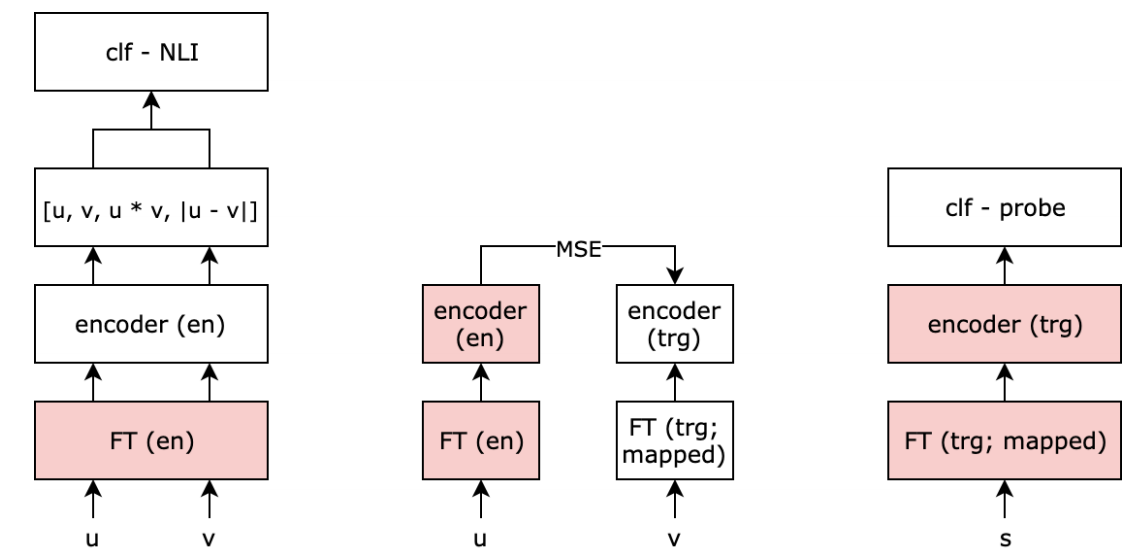
\includegraphics[scale=0.35]{images/x_probe}
	\caption[Encoder mapping procedure employed by Ravishankar and colleagues]
		{Illustration of the encoder mapping procedure employed by \citep{Ravishankar.2019}.
		The image was taken from \citep{Ravishankar.2019}}
	\label{fig:x_probe}
\end{figure}

\citep{Conneau.2018b} furthermore noticed that there was \textbf{no standard approach to the evaluation of sentence embeddings}. In each publication, different setups were used such that comparisons between individual results started to lack validity. As a consequence, they developed the \textit{SentEval} framework, an easy-to-use open-source Python project\footnote{\url{https://github.com/facebookresearch/SentEval} (retrieved: September 03, 2019)} which comes with diverse downstream classification tasks as well as the set of probing tasks introduced by \citep{Conneau.2018a}. \citep{Perone.2018} made use of this framework to conduct a comprehensive study in which they evaluated more state-of-the-art embedding architectures. Their experiments confirmed that there is no universal sentence embedding and furthermore showed that a \gls{bov} approach using contextualized \textit{ELMo} embeddings achieves high performance across many probing tasks.

Despite the convenient usage of such frameworks, \citep{Eger.2019} still notice several pitfalls that many researchers frequently tab into when it comes to probing sentence representations. These pitfalls include e.\,g. \textbf{using different classifier architectures} for the evaluation or \textbf{comparing sentence embeddings of different sizes}. The latter issue was already realized by \citep{Rueckle.2018} who pointed out that comparing usually low-dimensional average methods to higher-dimensional trained embeddings was unfair and therefore proposed to concatenate several average embeddings to increase their dimensionality. Finally, in order to facilitate a better evaluation, \citep{Eger.2019} conjecture that the set of downstream applications should be enriched with more demanding tasks where simple compositional models and random encoders are outperformed by trained encoder architectures more decisively.

\begin{tudbox}{Motivation and Goal of this Thesis}
\textbf{The above explanations show that the number of researchers taking a multi-lingual setting into account is small but increasing steadily. Nevertheless, the set of languages is still often limited to high-resource languages like German, French or Spanish. Overall, much less research could be found that focuses on probing sentence embeddings in lower-resource languages. It is therefore unclear whether the results obtained for high-resource languages are generalizable to languages for which by far less data is available. This circumstance makes it worthwhile to put lower-resource languages more in focus. Providing more insight into sentence embeddings in lower-resource languages is the goal of this thesis.}
\end{tudbox}

% -----------------------------------------------------------------------------------------------------------------------------------------------------
% Chapter Summary
\subsection{Summary}
\label{sec:rel_work_summary}

This chapter introduced the foundational work for this thesis. The literature review made clear that a large number of sentence embedding algorithms exists. However, large-scale evaluations of these techniques have long been neglected. What is more, before the release of \textit{SentEval}, no standard framework existed which could be used to assess the quality of the embeddings in a comparable way. Also, the probing task literature is mostly restricted to the English language, but successively, more and more researches are beginning to shift their focus to other languages which are morphologically richer than English. Most of the time only high-resource languages are taken into account, while low-resource languages are omitted. \textbf{This is why the present thesis aims to extend the probing task methodology to lower-resource languages in order to investigate whether the patterns found for high-resource languages are still reproducible if by far less resources are available.}

\newpage
% =======================
% Chapter: Word Embedding Algorithms
%
% Author: Daniel Wehner
%

% -----------------------------------------------------------------------------------------------------------------------------------------------------
\section{Word Embedding Algorithms}
\label{sec:word_embs}

\vspace*{-2mm}
% -----------------------------------------------------------------------------------------------------------------------------------------------------
% Chapter Introduction
\subsection{Introduction}
\label{sec:word_embs_intro}

Word embeddings form the basis for many sentence embedding algorithms. Therefore, this chapter introduces in more detail what word embeddings are, what approaches exist and how these approaches work. Section \vref{sec:w2v} introduces \textit{word2vec}, while the two subsequent sections are dedicated to \textit{FastText} and \textit{Attract-Repel}, respectively (cf. sections \vref{sec:fasttext} and \vref{sec:attract_repel}). The last section \vref{sec:word_embs_acquisition} finally shows how we acquired word embedding models for later experiments. Available pre-trained vectors were downloaded while others had to be trained from scratch. The section will also provide training details such as which values were used for the hyper-parameters of the respective models.

% -----------------------------------------------------------------------------------------------------------------------------------------------------
% Word2Vec
\subsection{Word2Vec}
\label{sec:w2v}

In order to learn dense word representations, \citep{Mikolov.2013a} introduced a neural approach they called \textit{word2vec}. This algorithm was considered a major breakthrough in the \gls{nlp} community by the time it was published. The learning process of \textit{word2vec} is guided by an \textbf{auxiliary task} which is inspired by language modeling \citep{Bengio.2003}. In contrast to language models which predict the next word in the sequence given all previous words, \textit{word2vec} either predicts the center word given the context words or the context words given the center word. The first variant is called \textit{\gls{cbow}}, while the second one is referred to as \textit{Skip-Gram}. The following paragraphs refer to the \textit{Skip-Gram} architecture, but the concepts are in general transferable to the \textit{\gls{cbow}} variant as well. Figure \vref{fig:skipgram_detail} provides a visual illustration of the explanations:

% Figure: Skip-gram model in detail
\begin{figure}[h]
	\centering
	\begin{tikzpicture}[
		scale=0.335,
		every node/.style={scale=0.7},
		box/.style={rounded corners,dashed}
	]

		%\node[rotate=90] at (-12,0) {\highlight{center word}};
		\node[rotate=90] at (37,0) {\highlight{context words}};

		\draw[box,fill=lightgray!10] (-11,-12) rectangle (-5,14);
		\draw[box,fill=lightgray!10] (-3,-12) rectangle (7,14);
		\draw[box,fill=lightgray!10] (9,-12) rectangle (15,14);

		\node[align=center] at (-8,12) {$\vert \mathcal{V} \vert \times 1$ \\ $\bm{\widehat{v}}_{w_c}$};
		\node[align=center] at (-8,-8) {\highlight{One-hot} \\ \highlight{word vector} \\ \highlight{center word}};

		\node[align=center] at (2,12) {$d \times \vert \mathcal{V} \vert$ \\ $\bm{E}$};
		\node[align=center] at (2,-8) {\highlight{Word embedding matrix}};

		\node[align=center] at (12,12) {$d \times 1$ \\ $\bm{v}_{w_c}$};
		\node[align=center] at (12,-8) {\highlight{Word emb.} \\ \highlight{for center word}};

		\node[align=center] at (19,14) {$\vert \mathcal{V} \vert \times d$ \\ $\bm{U}$};
		\node[align=center] at (25,14) {$\vert \mathcal{V} \vert \times 1$ \\ $\bm{u}_{w_o}^{\intercal} \bm{v}_{w_c}$};
		\node[align=center] at (30,14) {$\vert \mathcal{V} \vert \times 1$ \\ soft-max};
		\node[align=center] at (35,14) {$\vert \mathcal{V} \vert \times 1$ \\ truth};

		\node at (-4,0) {\Large $\times$};
		\node at (8,0) {\Large $=$};

		\node at (-8,0) {$\begin{bmatrix} 0 \\ 0 \\ 0 \\ 0 \\ 0 \\ 1 \\ 0 \\ 0 \\ 0 \end{bmatrix}$};
		\node at (2,0) {$
			\begin{bmatrix*}[r]
				\bullet 	& \hdots 	& 0.2 	& \hdots & \bullet \\[3.2mm]
				\bullet 	& \hdots 	& -1.4 	& \hdots & \bullet \\[3.2mm]
				\bullet 	& \hdots 	& 0.3 	& \hdots & \bullet \\[3.2mm]
				\bullet 	& \hdots 	& -0.1 	& \hdots & \bullet \\[3.2mm]
				\bullet 	& \hdots 	& 0.1 	& \hdots & \bullet \\[3.2mm]
				\bullet 	& \hdots 	& 0.5 	& \hdots & \bullet
			\end{bmatrix*}$};
		\node at (12,0) {$
			\begin{bmatrix*}[r]
				0.2 	\\[3.2mm]
				-1.4	\\[3.2mm]
				0.3 	\\[3.2mm]
				-0.1	\\[3.2mm]
				0.1 	\\[3.2mm]
				0.5
			\end{bmatrix*}$};

			\draw[thick] (16,-3.5) rectangle (22,3.7);
			\draw[thick] (16,-3.5) -- (22,5) -- (22,12.2) -- (16,3.7);
			\draw[thick] (16,3.7) -- (22,-5) -- (22,-12.2) -- (16,-3.5);

		\node at (25,8.75) {$
			\begin{bmatrix*}[r]
				0.2 		\\[3.2mm]
				0.3		\\[3.2mm]
				0.1 		\\[3.2mm]
				\vdots 	\\[3.2mm]
				0.7
			\end{bmatrix*}$};

		\node at (30,8.75) {$
			\begin{bmatrix*}[r]
				0.08 	\\[3.2mm]
				0.10	\\[3.2mm]
				0.05 	\\[3.2mm]
				\vdots 	\\[3.2mm]
				\textcolor{tud9c}{0.65}
			\end{bmatrix*}$};
			\node at (35,8.75) {$\begin{bmatrix} 0 \\[3.2mm] 0 \\[3.2mm] 0 \\[3.2mm] \vdots \\[3.2mm] \textcolor{tud9c}{1} \end{bmatrix}$};
			
		\node at (25,0.1) {$
			\begin{bmatrix*}[r]
				0.7 		\\[3.2mm]
				0.3		\\[3.2mm]
				0.1 		\\[3.2mm]
				\vdots 	\\[3.2mm]
				-0.1
			\end{bmatrix*}$};

		\node at (30,0.1) {$
			\begin{bmatrix*}[r]
				\textcolor{tud9c}{0.65} 	\\[3.2mm]
				0.10	\\[3.2mm]
				0.05 	\\[3.2mm]
				\vdots 	\\[3.2mm]
				0.03
			\end{bmatrix*}$};
			\node at (35,0.1) {$\begin{bmatrix} 0 \\[3.2mm] \textcolor{tud9c}{1} \\[3.2mm] 0 \\[3.2mm] \vdots \\[3.2mm] 0 \end{bmatrix}$};

		\node at (25,-8.75) {$
			\begin{bmatrix*}[r]
				0.5 		\\[3.2mm]
				0.7		\\[3.2mm]
				0.1		\\[3.2mm]
				\vdots 	\\[3.2mm]
				0.4
			\end{bmatrix*}$};

		\node at (30,-8.75) {$
			\begin{bmatrix*}[r]
				\textcolor{tud9c}{0.40} 	\\[3.2mm]
				0.15	\\[3.2mm]
				0.05 	\\[3.2mm]
				\vdots 	\\[3.2mm]
				0.30
			\end{bmatrix*}$};
			\node at (35,-8.75) {$\begin{bmatrix} 0 \\[3.2mm] 0 \\[3.2mm] 0 \\[3.2mm] \vdots \\[3.2mm] \textcolor{tud9c}{1} \end{bmatrix}$};

	\end{tikzpicture}
	\caption[Word2vec's skip-gram model architecture in detail]{The Skip-gram model in detail.
		Image taken and adapted from Manning: \url{https://www.youtube.com/watch?v=ERibwqs9p38}
		(Lecture recording from Stanford university; retrieved: September 04, 2019).}
	\label{fig:skipgram_detail}
\end{figure}

Given the center word $w_c^{(t)}$ at time step $t$, the \textit{Skip-Gram} model has to predict the surrounding words which are given by a sliding window of size $m$ centered on $w_c^{(t)}$. To this end, $w_c^{(t)}$ which is represented as a one-hot vector $\bm{\widehat{v}}_{w_c^{(t)}} \in \mathbb{R}^{\vert \mathcal{V} \vert \times 1}$, is first multiplied by a shared embedding matrix $\bm{E} \in \mathbb{R}^{d \times \vert \mathcal{V} \vert}$, where $d$ is the desired dimensionality of the resulting word embeddings. This matrix contains the weights of the network connecting the input layer to the single hidden layer (with identity activation). The weights in matrix $E$ represent the word embeddings once the model is fully trained. Since the input vector has the one-hot property, the vector-matrix multiplication retrieves one specific column from the matrix, namely the respective (intermediate) embedding of the center word $\bm{v}_{w_c^{(t)}}$.

\textbf{The model must be provided with a supervision signal} in order to adjust the weights during training. In machine learning, this signal is usually obtained by comparing the predictions of the model with the desired output (supervised learning). This results in a training loss whose value is dependent on how far off the model was with its predictions. Based on the loss, the model parameters are adjusted to a greater or lesser extent. However, the training corpus does not have any dedicated labels in this context. Instead, the words in the corpus themselves are used. This approach can be considered a mixture of supervised and unsupervised learning which is commonly known as \textbf{self-supervision}. The labels which are used by \textit{Skip-Gram} are given by the one-hot vectors of the respective context words. To obtain the prediction of the model, one must further multiply the center word embedding by a matrix $\bm{U} \in \mathbb{R}^{\vert \mathcal{V} \vert \times d}$. The resulting vector then serves as input to a soft-max activation which yields a probability distribution over all possible words in the vocabulary $\mathcal{V}$. To be more precise, each word has two representations: One center word representation (contained in matrix $\bm{E}$) and a context word representation (contained in matrix $\bm{U}$). Matrix $\bm{U}$ is needed only for the training procedure and is discarded in the end. During training, the \textit{Skip-Gram} architecture attempts to \textbf{maximize the negative log-probability of the context words given the center word}:

\vspace*{-6mm}
\begin{align}
	\mathcal{J}(\bm{\theta})
		&= -\frac{1}{T} \sum_{t=1}^T \sum_{\substack{-m \le j \le m \\ j \ne 0}}
			\log p(w^{(t+j)} \vert w_c^{(t)}; \bm{\theta}), \\
	\intertext{where the probability is given by the soft-max activation:}
	p(o \vert c)
		&= \frac{\exp\{ \bm{u}_{w_o}^{\intercal} \bm{v}_{w_c}\}}{
			\sum_{\ell=1}^{\vert \mathcal{V} \vert} \exp\{ \bm{u}_{w_\ell}^{\intercal} \bm{v}_{w_c}\}}.
\end{align}
\vspace*{-2mm}

Vector $\bm{\theta}$ denotes the parameters of the model. In this case these are the entries of the matrices $\bm{E}$ and $\bm{U}$. $T$ is the number of words in the training corpus whereas $t$ represents the index into the training corpus. The latter must not be confused with $o$ (context) and $c$ (center) which are indices into the vocabulary $\mathcal{V}$. $\bm{u}_{w_o}^{\intercal} \bm{v}_{w_c}$ is called the scoring function $s(c, o)$.

One property of \textit{word2vec} is that the learned embeddings do not only capture \textbf{syntactical features} of natural language, but incorporate \textbf{semantic aspects} of words as well. \citep{Mikolov.2013c} detected this desirable property by defining nine syntactic and five semantic tasks/questions, e.\,g. \texttt{Adjective-Adverb} (syntactic) or \texttt{Man-Woman} (semantic). The task is to answer questions like \textit{`What is the word that is related to king in the same sense as man is related to woman?'}. The authors were able to demonstrate that such questions can be answered by performing simple algebraic operations on the corresponding word vectors: $\bm{v}_{king} - \bm{v}_{man} + \bm{v}_{woman} \approx \bm{v}_{queen}$ (cf. figure \vref{fig:word2vec_vector_operations}).

\begin{figure}[h]
  	\centering
    	\begin{tikzpicture}[
	scale=0.5,
	every node/.style={scale=0.8},
	arr/.style={-stealth,thick}
]
	
	\node (M) at (0,0) {Man};
	\node (W) at (2,2) {Woman};
	\draw[arr,blue] (M) -- (W);
	
	\node (U) at (3,0) {Uncle};
	\node (A) at (5,2) {Aunt};
	\draw[arr,blue] (U) -- (A);
		
	\node (K1) at (-0.5,-3) {King};
	\node (Q1) at (1.5,-1) {Queen};
	\draw[arr,blue] (K1) -- (Q1);

	\draw[dashed,thick] (7.5,2) -- (7.5,-3);

	\node (K2) at (12,-3) {King};
	\node (Ks) at (10,0) {Kings};
	\node (Q2) at (14,-1) {Queen};
	\node (Qs) at (12,2) {Queens};

	\draw[arr,red] (K2) -- (Ks);
	\draw[arr,red] (Q2) -- (Qs);
	\draw[arr,blue] (K2) -- (Q2);
\end{tikzpicture}
	
  	\caption[Evaluation of word embeddings using similarity tasks]
  	{Similarity tasks can be solved by performing simple algebraic vector operations. The image was taken and adapted from
	\citep{Mikolov.2013c}.}
	\label{fig:word2vec_vector_operations}
\end{figure}

% -----------------------------------------------------------------------------------------------------------------------------------------------------
% FastText
\subsection{FastText}
\label{sec:fasttext}

Despite the great impact \textit{word2vec} had, \citep{Bojanowski.2017} could identify drawbacks. The authors observed that \textbf{the algorithm treats words as atomic units}. This design choice entails problems for words not contained in the training corpus. A large amount of \textbf{\gls{oov} words} is the consequence. It is particularly difficult to learn robust word embeddings for morphologically rich languages like e.\,g. Turkish. In order to address this issue, \citep{Bojanowski.2017} \textbf{enrich the \textit{Skip-Gram} model with sub-word information, where words are considered bags of character $n$-grams}. The word embedding is then defined as the sum of the respective $n$-gram embeddings. Given that the training corpus is sufficiently large, this method basically avoids any \gls{oov} words. If a word did not exist in the training data, its embedding can nevertheless be obtained by summing the respective $n$-gram embeddings. \citep{Bojanowski.2017} were inspired by \citep{Schuetze.1993} and \citep{Wieting.2016a} who introduced similar concepts.

In order to formalize this idea, let $w$ denote an arbitrary word in the vocabulary $\mathcal{V}$. $\mathcal{G}_w$ denotes the set of $n$-grams the word $w$ consists of. A dedicated vector representation $\bm{z}$ is learned for each $n$-gram appearing in the training corpus. \citep{Bojanowski.2017} subsequently replace the original scoring function of \textit{word2vec} by the sum of all character $n$-grams of $w$:

\begin{equation}
	s(c, o) = \sum_{g \in \mathcal{G}_{w_c}} \bm{z}_g^{\intercal} \bm{u}_{w_o}
\end{equation}

The inventors of \textit{FastText} suggest that $n$ be chosen to be in the range from 3 to 6. The authors present an example: Let $n$ be set to 3. The $n$-grams of the word \textit{`where'} are given by: \texttt{<wh}, \texttt{whe}, \texttt{her}, \texttt{ere}, \texttt{re>}. Before the creation of the $n$-grams a word is enclosed in angle brackets (\texttt{<...>}).

% -----------------------------------------------------------------------------------------------------------------------------------------------------
% Attract-Repel
\subsection{Attract-Repel}
\label{sec:attract_repel}

\citep{Mrksic.2017} suggest to incorporate linguistic constraints into the learning process to improve the quality of the word embeddings. Examples for such constraints are \textbf{synonymy/antonymy relationships} between words. Synonymy constraints are introduced to reduce the distance between embeddings representing words with a similar meaning (\textit{attract}) while antonymy relationships allow for pushing vectors further away from each other if the words they represent have contradictory meanings (\textit{repel}). Such relationships can be obtained from lexical resources like e.\,g. \textit{WordNet} \citep{Miller.1995}. In general, two approaches exist how such additional constraints can be incorporated into the process of embedding creation: \ding{182} \textbf{By training word vectors from scratch while respecting the linguistic constraints} or \ding{183} \textbf{by reusing existing word representations which are fine-tuned such that the embeddings obey these constraints}. The authors call this procedure \textbf{semantic specialization}. \textit{Attract-Repel} implements the latter approach and was inspired by techniques called \textit{retro-fitting} \citep{Faruqui.2015}, \textit{Paragram} \citep{Wieting.2015} and \textit{counter-fitting} \citep{Mrksic.2016}.

The inventors of \textit{Attract-Repel} define $S$ and $A$ to be the sets of synonymous and antonymous word pairs, respectively. $(\bm{x}_l, \bm{x}_r)$ describes such a pair, where the words are given by their corresponding vectorial representations. In each training iteration, one mini-batch $\mathcal{B}$ is used consisting of $k_1$ synonymous word pairs ($\mathcal{B}_S$) and $k_2$ antonymous word pairs ($\mathcal{B}_A$). Let further denote $\mathcal{N}_S = \{ (\bm{t}_l^1, \bm{t}_r^1), \dots, (\bm{t}_l^{(k_1)}, \bm{t}_r^{(k_1)}) \}$ the set of negative examples for the synonymous word pairs. A similar set $\mathcal{N}_A = \{ (\bm{t}_l^1, \bm{t}_r^1), \dots, (\bm{t}_l^{(k_2)}, \bm{t}_r^{(k_2)}) \}$ be defined for the antonymous pairs. \\
The negative counterpart of a word pair $(\bm{x}_l, \bm{x}_r)$ is selected from the other words in batch $\mathcal{B}$. For synonymous word pairs, $\bm{t}_l$ is the nearest neighbor of $\bm{x}_l$, while $\bm{t}_r$ is the nearest neighbor of $\bm{x}_r$. Similarly, for antonymous word pairs, $\bm{t}_l$ is selected to be the vector with the largest distance to $\bm{x}_l$, while $\bm{t}_r$ is the vector with the largest distance to $\bm{x}_r$. The cost function of the model is given by:

\begin{align}
	\label{eq:cost_syn}
	\mathcal{J}(\mathcal{B}_S)
		&=\sum_{(\bm{x}_l, \bm{x}_r) \in \mathcal{B}_S}
			\big(\tau(\delta_{syn} + \bm{x}_l^{\intercal} \bm{t}_l - \bm{x}_l^{\intercal} \bm{x}_r) +
			\tau(\delta_{syn} + \bm{x}_r^{\intercal} \bm{t}_r - \bm{x}_l^{\intercal} \bm{x}_r)\big) \\
	\label{eq:cost_ant}
	\mathcal{J}(\mathcal{B}_A) 
		&=\sum_{(\bm{x}_l, \bm{x}_r) \in \mathcal{B}_A}
			\big(\tau(\delta_{ant} + \bm{x}_l^{\intercal} \bm{x}_r - \bm{x}_l^{\intercal} \bm{t}_l) +
			\tau(\delta_{ant} + \bm{x}_l^{\intercal} \bm{x}_r - \bm{x}_r^{\intercal} \bm{t}_r)\big) \\
	\mathcal{J}(\mathcal{B})
		&= \mathcal{J}(\mathcal{B}_S) + \mathcal{J}(\mathcal{B}_A) + \text{regularization term}
\end{align}

$\tau(x)$ denotes the \textbf{hinge loss} and $\delta_{syn}$ is a hyper-parameter specifying how much closer the synonymous words should be in contrast to the negative examples ($\delta_{ant}$ is defined analogously for antonymous word pairs). For intuition, consider equation \vref{eq:cost_syn} which shows the part of the cost function concerning synonymous constraints. If $\bm{x}_l$ and $\bm{x}_r$ are nearby vectors, their dot product will be large. This is desirable, since the two words are synonymous. Subtracting this quantity reduces the cost. At the same time, a large dot product of $\bm{x}_l$ with its negative example $\bm{t}_l$ is punished by adding the respective term. In their experiments the authors minimize the objective function using the \textbf{AdaGrad} optimization technique \citep{Duchi.2011}. Training for five epochs without early stopping was found to be sufficient to obtain sensibly fine-tuned word representations. The authors could produce significant quality improvements for low-resource languages and observed enhanced performance in downstream tasks.

% -----------------------------------------------------------------------------------------------------------------------------------------------------
% Acquisition of Word Embeddings
\subsection{Acquisition of Word Embeddings}
\label{sec:word_embs_acquisition}

The word embeddings presented in this chapter play an important role, since they form the basis for sentence embedding algorithms which will be covered in  chapter \vref{sec:sent_embs}. Table \vref{tab:word_embs_acquisition} summarizes how these word embeddings were obtained:

% Table: Overview word embeddings
\vspace*{2mm}
\begin{table}[h]
	\centering
	\renewcommand{\arraystretch}{2.2}
	\scalebox{1.0}{
	\begin{tabularx}{0.95\textwidth}{| c | X | c | c | c | c | c | c | c | c | c |}
		\hline
		\cellcolor{tud9c!50}							 								&
		\cellcolor{tud9c!50}															&
		\multicolumn{5}{c |}{\cellcolor{tud9c!50}\textbf{Embedding source}}	 			&
		\cellcolor{tud9c!50}								 							&
		\multicolumn{3}{c |}{\cellcolor{tud9c!50}\textbf{Training details}}				\\
		\cellcolor{tud9c!50}\multirow{-2}{*}{\textbf{Nr.}}								&
		\cellcolor{tud9c!50}\multirow{-2}{*}{\textbf{Embedding}}						&
		\cellcolor{tud9c!30}\textbf{EN} 												&
		\cellcolor{tud9c!30}\textbf{DE} 												&
		\cellcolor{tud9c!30}\textbf{RU} 												&
		\cellcolor{tud9c!30}\textbf{TR} 												&
		\cellcolor{tud9c!30}\textbf{KA} 												&
		\cellcolor{tud9c!50}\multirow{-2}{*}{\textbf{Download}}							&
		\cellcolor{tud9c!30}\textbf{Dimen.}			 									&
		\cellcolor{tud9c!30}\textbf{Window size} 										&
		\cellcolor{tud9c!30}\textbf{Architecture}										\\
		\hline\hline

		% word2vec
		\ding{182} 																	&
		\textit{word2vec} 															&
		\faDownload 																	&
		\faDownload																	&
		\faCogs 																		&
		\faCogs																		&
		\faCogs																		&
		\href{https://code.google.com/archive/p/word2vec/}{\linkstyle{Link1}},
		\href{https://deepset.ai/german-word-embeddings}{\linkstyle{Link2}}				&
		300																			&
		10 																			&
		CBOW 
																					\\
		% fastText
		\ding{183} 																	&
		\textit{FastText}																&
		\faDownload 																	&
		\faDownload 																	&
		\faDownload 																	&
		\faDownload 																	&
		\faDownload																	&
		\href{https://fasttext.cc/docs/en/crawl-vectors.html}{\linkstyle{Link}}				&
		300																			&
		- 																			&
		- 
																					\\
		% attract-repel
		\ding{184} 																	&
		\textit{Attract-Repel}															&
		\faDownload 																	&
		\faDownload 																	&
		\faDownload 																	&
		\faDownload 																	&
		\faDownload																	&
		\href{https://drive.google.com/drive/folders/0B_pyA_IW4g-jZHlWWVBfaWRYY0E}
			{\linkstyle{Link}}															&
		300																			&
		- 																			&
		- 																			\\
		\hline
	\end{tabularx}}
	\caption[Sources of word embeddings]{Overview of word embedding acquisition.
		The \faDownload\ symbol indicates that the model was downloaded, whereas the \faCogs\ symbol refers to
		a trained model.}
	\label{tab:word_embs_acquisition}
\end{table}
\vspace*{2mm}
 
\highlight{Availability of pre-trained word embeddings.} Pre-trained embedding spaces for \textit{FastText} and \textit{Attract-Repel} are already publicly available for all target languages. These word vectors were thus downloaded from the respective sources (indicated by the \faDownload\ symbol in table \vref{tab:word_embs_acquisition}). We found \textit{word2vec} vectors for English and German, but unfortunately not for Georgian. This is why we trained these embeddings from scratch (indicated by the \faCogs\ symbol in table \vref{tab:word_embs_acquisition}). For Turkish, only 200-dimensional vectors were available. Different embedding dimensionalities render the results less comparable as already pointed out by \citep{Eger.2019}. Therefore, we chose to train Turkish embeddings as well. Although trained vector representations exist for Russian, we decided to proceed analogously, in order to have similar conditions among the low-resource languages.

\highlight{Training details.} We trained all \textit{word2vec} embeddings on Wikipedia dumps for the respective languages (Russian, Turkish and Georgian). The dumps are provided by Wikimedia\footnote{\url{https://dumps.wikimedia.org/} (retrieved: September 20, 2019)} in an \gls{xml} format. In order to get hold of the plain text which is needed for training, these \gls{xml} files have to be parsed. A module for the Python programming language called  \texttt{WikiExtractor}\footnote{\url{https://github.com/attardi/wikiextractor} (retrieved: September 20, 2019)} was used for this purpose. Table \vref{tab:wikipedia_stats} shows the sizes of the Wikipedia dumps as measured by the number of sentences.

Mikolov and colleagues provide the official C-implementation of \textit{word2vec} on GitHub\github.\footnote{\url{https://github.com/tmikolov/word2vec} (retrieved: September 20, 2019)} For training, we did not change the default hyper-parameters of the script. The training setting is as follows: First of all, the \textit{\gls{cbow}} architecture was used and the window size was set to $m = 10$. We chose a dimensionality of the resulting vectors of $d = 300$. The training process took about 2 hours per language on a \gls{gpu} computer, where the reduced amount of training time is due to smaller data sets as can be seen in table \vref{tab:wikipedia_stats}.

\begin{table}[h]
	\centering
    	\renewcommand{\arraystretch}{1.2}
\scalebox{1.05}{
\begin{tabular}{| c | r | c |}
	\hline
	\rowcolor{tud9c!50}
	\textbf{Language}	&
	\textbf{\# sentences} & 
	\textbf{Version} \\
	\hline\hline
	\textbf{English} 		& 	97,285,870 	&	20.02.2019 	\\
	\textbf{German} 		& 	40,729,339	&	20.09.2018	\\
	\textbf{Russian} 		& 	25,324,234 	&	01.02.2019	\\
	\textbf{Turkish} 		& 	3,797,955	&	01.01.2019	\\
	\textbf{Georgian} 	& 	1,047,780	&	20.07.2016	\\
	\hline
\end{tabular}}
  	\caption[Wikipedia statistics for each language]
		{Number of sentences contained in the Wikipedia dumps for each language. As can be seen, among the languages
 		considered Georgian is by far the one with the fewest resources.}
	\label{tab:wikipedia_stats}
\end{table}

% -----------------------------------------------------------------------------------------------------------------------------------------------------
% Chapter Summary
\subsection{Summary}
\label{sec:word_embs_summary}

In this chapter the concept of word embeddings was introduced. Since most machine learning algorithms are not designed for natural language input, researchers began to devise techniques to obtain vectorial representations of language which are called language embeddings. Mikolov and colleagues introduced a seminal approach they called \textit{word2vec}. It can be trained efficiently on large corpora and captures not only syntactic but also semantic aspects of words. The fact that simple algebraic operations on these vectors suffice to answer similarity questions popularized this algorithm in the \gls{nlp} community.

To account for some drawbacks of the \textit{word2vec} algorithm, other techniques and extensions were proposed. \textit{FastText} extends the \textit{Skip-Gram} model to character $n$-grams which enables it to cope with \gls{oov}-words in a more graceful fashion. \textit{Attract-Repel} explicitly includes linguistic constraints based on synonymy and antonymy relationships to fine-tune existing word embeddings. The idea behind this approach is that synonymous words should be mapped close to each other in the embedding space while antonymous words should be as far apart as possible.

Finally, an overview provided information about where and how the word embeddings were obtained. Pre-trained models for \textit{FastText} and \textit{Attract-Repel} embeddings were available for all target languages and were therefore downloaded from the official websites. Suitable \textit{word2vec} vectors were available only for English and German. For the low-resource languages Russian, Turkish and Georgian they were trained from scratch using the official implementation provided by Mikolov and colleagues.
\newpage
% =======================
% Chapter: Sentence Embedding Algorithms
%
% Author: Daniel Wehner
%

% -----------------------------------------------------------------------------------------------------------------------------------------------------
\section{Sentence Embedding Algorithms}
\label{sec:sent_embs}

\vspace*{-0.5mm}
% -----------------------------------------------------------------------------------------------------------------------------------------------------
% Chapter Introduction
\subsection{Introduction}
\label{sec:sent_embs_intro}

Due to the significant impact word embeddings had on the performance of machine learning techniques in the context of \gls{nlp}, the question arose whether it is possible to encode even larger spans of text in terms of a single vector. \citep{Le.2014} were among the first researchers to introduce embeddings for sentences, paragraphs and even entire documents. This chapter gives an introduction to common sentence embedding algorithms. \citep{Yang.2018} distinguish between two major approaches: They differentiate between \textbf{non-parameterized} methods which combine underlying word embeddings and \textbf{parameterized} methods which train sentence embeddings from scratch. Table \vref{tab:sent_embs_types} gives an overview of common algorithms (\textit{not exhaustive}):

% Table: Types and examples of sentence embeddings
\vspace*{3mm}
\begin{table}[h]
	\centering
	\renewcommand{\arraystretch}{1.4}
	\scalebox{0.95}{
	\begin{tabularx}{\textwidth}{| X | l ? X | l |}
		\hline
		\multicolumn{2}{| c ?}{
			\cellcolor{tud9c!50}
				\textbf{Non-parameterized methods}}				&
		\multicolumn{2}{ c |}{
			\cellcolor{tud9c!50}
				\textbf{Parameterized methods}} 					\\
		\rowcolor{tud9c!30}
		\textbf{Algorithm} 										&
		\textbf{Source} 											&
		\textbf{Algorithm} 										&
		\textbf{Source}											\\
		\hline\hline

		\ding{182} \textit{Vanilla average}							&
		\textit{- no author found -}								&
		\ding{182} \textit{Skip-Thought} 							&
		\citep{Kiros.2015} 									\\
		\hline

		\ding{183} \textit{Concatenated $p$-means}				&
		\citep{Rueckle.2018}										&
		\ding{183} \textit{Quick-Thought}							&
		\citep{Logeswaran.2018}									\\
		\hline

		\ding{184} \textit{\gls{gem}}		 						&
		\citep{Yang.2018} 										&
		\ding{184} \textit{sent2vec}								&
		\citep{Pagliardini.2018}									\\
  		\hline

		\ding{185} \textit{\gls{sif}}	 							&
		\citep{Arora.2017}										&
		\ding{185} \textit{InferSent} 								&
		\citep{Conneau.2017} 									\\
  		\hline

		\cellcolor{lightgray!50}		 							&
		\cellcolor{lightgray!50}		 							&
		\ding{186} \textit{\gls{sbert}} 								&
		\citep{Reimers.2019} 										\\
  		\hline

		\cellcolor{lightgray!50}		 							&
		\cellcolor{lightgray!50}		 							&
		\ding{187} \textit{\gls{laser}} 								&
		\citep{Artetxe.2018} 										\\
  		\hline
	\end{tabularx}}
	\caption[Types and examples of sentence embedding algorithms]
	{Types and examples of sentence embedding algorithms.
		Non-parameterized methods combine existing word embeddings to obtain a sentence representation
		whereas parameterized methods train sentence embeddings from scratch.}
	\label{tab:sent_embs_types}
\end{table}
\vspace*{3mm}

The rest of this chapter is organized as follows: Section \vref{sec:sent_embs_non_param} introduces some examples of non-parameterized algorithms which are going to be used in the experiments. Section \vref{sec:sent_embs_param} then presents their parameterized counterparts. Analogously to the previous chapter, details are given where and how the individual sentence encoders were obtained (cf. section \vref{sec:sent_embs_acquisition} for more information).

% -----------------------------------------------------------------------------------------------------------------------------------------------------
% Non-parameterized Sentence Embeddings
\subsection{Non-parameterized Sentence Embeddings / Compositional Models}
\label{sec:sent_embs_non_param}

\vspace*{-1mm}
% -----------------------------------------------------------------------------------------------------------------------------------------------------
% Vanilla Average
\subsubsection{Vanilla Average}
\label{sec:vanilla_average}

The most straightforward approach to generate a sentence representation is the \textit{vanilla average} technique. The embeddings of the words in the sentence to be encoded are averaged using a simple \textbf{arithmetic mean}: $\bm{v}_s = \frac{1}{T} \sum_{t=1}^T \bm{v}_{w_t}$, where $T$ denotes the length of the sentence. While this approach is very intuitive and easy to implement, it has severe shortcomings: \ding{182} It \textbf{neglects the word order}, therefore it is also referred to as a \gls{bow} approach. \ding{183}\,Furthermore, \textbf{stop-words and more informative words are weighted equally} \citep{Le.2014}. Figure \vref{fig:mean_sentence_embedding} shows an exemplary sentence:

% Figure: Example for mean sentence embeddings
\begin{figure}[h]
	\centering
	\begin{tikzpicture}[
		scale=0.7,
		every node/.style={scale=0.7},
		arr/.style={stealth-stealth,double}
	]

		\node at (-3,0) {\Large $w_t$};
		\node (w1) at (0,0) {\strut\large\textbf{One}};
		\node (w2) at (3,0) {\strut\large\textbf{ring}};
		\node (w3) at (6,0) {\strut\large\textbf{to}};
		\node (w4) at (9,0) {\strut\large\textbf{rule}};
		\node (w5) at (12,0) {\strut\large\textbf{them}};
		\node (w6) at (15,0) {\strut\large\textbf{all}};
		\node (w7) at (18,0) {\strut\large\textbf{.}};

		\node at (-3,-3) {\Large $\bm{v}_{w_t}$};
		\node (v1) at (0,-3) {$\begin{bmatrix} 5.04 \\ -3.45 \\ \vdots \\ 0.06 \end{bmatrix}$};
		\node (v2) at (3,-3) {$\begin{bmatrix} 0.34 \\ 1.08 \\ \vdots \\ -5.87 \end{bmatrix}$};
		\node (v3) at (6,-3) {$\begin{bmatrix} -0.05 \\ 2.46 \\ \vdots \\ -1.34 \end{bmatrix}$};
		\node (v4) at (9,-3) {$\begin{bmatrix} -7.83 \\ 0.27 \\ \vdots \\ 3.36 \end{bmatrix}$};
		\node (v5) at (12,-3) {$\begin{bmatrix} -8.92 \\ -0.32 \\ \vdots \\ -3.74 \end{bmatrix}$};
		\node (v6) at (15,-3) {$\begin{bmatrix} -9.21 \\ 0.93 \\ \vdots \\ -0.05 \end{bmatrix}$};
		\node (v7) at (18,-3) {$\begin{bmatrix} -4.12 \\ 3.57 \\ \vdots \\ 1.06 \end{bmatrix}$};

		\draw[arr] (w1) -- (v1);
		\draw[arr] (w2) -- (v2);
		\draw[arr] (w3) -- (v3);
		\draw[arr] (w4) -- (v4);
		\draw[arr] (w5) -- (v5);
		\draw[arr] (w6) -- (v6);
		\draw[arr] (w7) -- (v7);

	\end{tikzpicture}
	\caption[Vanilla average: A simple example]
		{An example of a sentence of length seven ($T = 7$). The single word vectors are averaged in order to
		obtain a sentence embedding.}
	\label{fig:mean_sentence_embedding}
\end{figure}

\textit{Vanilla average} sentence embeddings are commonly used as a baseline. More sophisticated algorithms should be able to outperform this na\"{i}ve method. In fact, this algorithm is an instantiation of a more general family of algorithms which \citep{Shen.2018} call \glspl{swem}. An arithmetic mean is not the only pooling mechanism which can be applied. Other strategies include \textit{min-pooling}, \textit{max-pooling} or \textit{hierarchical pooling}. The latter technique makes use of a sliding window which is shifted over the input sentence, where all word representations in the window are pooled until finally, the resulting pooled vectors for each window are in turn combined to form the ultimate sentence vector.

% -----------------------------------------------------------------------------------------------------------------------------------------------------
% Concatenated Power Means
\subsubsection{Concatenated Power Means}
\label{sec:concat_p_means}

\citep{Rueckle.2018} propose to generalize the idea of average sentence embeddings to a concatenation of several power-means. The concatenation aims to capture more information about the sentence structure and is an attempt to make the comparison to trained models fairer. As was found by the authors, more complex and high-dimensional models like \textit{InferSent} are often directly compared to lower-dimensional average embeddings. Equation \vref{eq:p_mean} depicts the general form of a power mean. The equation introduces a hyper-parameter $p$ which specifies the type of average to be computed. As can directly be seen, the arithmetic mean is obtained by setting $p = 1$. Different values for $p$ yield different means. E.\,g. if $p = -1$, the output of the formula is the \textbf{harmonic mean}. For $p$ approaching (negative) $\infty$ the result is going to be the \textbf{maximum} (\textbf{minimum}) of the input data. The following paragraphs describe how this idea can be used to generate sentence embeddings which are more expressive.

\begin{equation}
	\label{eq:p_mean}
	\overline{x} = \left[ \frac{x_1^p + x_2^p + \dots + x_T^p}{T} \right]^{\nicefrac{1}{p}}
\end{equation}

Let $\bm{S}^{(j)} = [\bm{v}_{w_1}^{(j)}, \bm{v}_{w_2}^{(j)}, \dots, \bm{v}_{w_T}^{(j)}] \in \mathbb{R}^{d_j \times T}$ be the embedding matrix of a sentence $s = \langle w_1, w_2, \dots, w_T \rangle$ of length $T$. $j$ is the index variable into the set of $l$ embedding spaces $\mathbb{E} = \{ \mathbb{E}^{(j)} \}_{j=1}^l$ and $d_j$ denotes the dimensionality of the word embeddings in the respective embedding spaces. $\mathbb{E}^{(j)}$ contains all word vectors that were trained by the same method. For example all \textit{word2vec} vectors constitute one embedding space whereas all \textit{FastText} vectors lie in a different embedding space. Further, let $f_p(\bm{S}^{(j)})$ with $f_p: \mathbb{R}^{d_j \times T} \mapsto \mathbb{R}^{d_j}$ be a mapping of a sentence embedding matrix to a single $p$-mean vector. The sentence representation for one embedding space is computed by applying function $f_p$ $k$ times with different values for $p$ and successively concatenating the results (concatenation is denoted by the $\oplus$ symbol): $\bm{v}_{s}^{(j)} = f_{p_1}\left(\bm{S}^{(j)}\right) \oplus f_{p_2}\left(\bm{S}^{(j)}\right) \oplus \dots \oplus f_{p_k}\left(\bm{S}^{(j)}\right)$. The ultimate sentence embedding $\bm{v}_s$ is generated by concatenating the representations from all embedding spaces $\mathbb{E}^{(j)}$.

% -----------------------------------------------------------------------------------------------------------------------------------------------------
% Parameterized Sentence Embeddings
\subsection{Parameterized Sentence Embeddings / Trained Encoders}
\label{sec:sent_embs_param}

% -----------------------------------------------------------------------------------------------------------------------------------------------------
% SkipThought
\subsubsection{Skip-Thought and Quick-Thought}
\label{sec:skipthought}

\highlight{Skip-Thought.} Inspired by the \textit{Skip-Gram} model, \citep{Kiros.2015} proposed a sentence embedding algorithm named \textit{Skip-Thought}. Given a sentence $s_i$, the model's objective in the training phase is to predict the two neighboring sentences $s_{i-1}$ and $s_{i+1}$, respectively. Thus, the input to the model consists of a tuple of three sentences which have to be taken from an \textbf{ordered corpus}, i.\,e. nearby sentences have to be related. For example consider the following three sentences:

\begin{center}
	\colorbox{lightgray!15}{$\langle$ \textbf{I got back home} $\rangle_{s_{i-1}}$},
	\colorbox{tud9c!15}{$\langle$ \textbf{I could see the cat on the steps} $\rangle_{s_i}$} and
	\colorbox{lightgray!15}{$\langle$ \textbf{This was very strange} $\rangle_{s_{i+1}}$}
\end{center}

Especially well suited are book corpora which provide large amounts of contiguous text. \citep{Kiros.2015} trained the model on the \textit{BookCorpus} data set by \citep{Zhu.2015}. The training corpus is not annotated, hence \textit{Skip-Thought} belongs to the family of unsupervised machine learning algorithms. Figure \vref{fig:skipthought_architecture} depicts the model architecture: The middle sentence $s_i$ (\textit{`I could see the cat on the steps')} is first encoded into a compact representation $\bm{h}_i$ which is then passed on to two separate decoders which predict the surrounding sentences $s_{i-1}$ (\textit{`I got back home'}) and $s_{i+1}$ (\textit{`This was very strange'}). At each decoding step, the model is fed with its output one time step in the past as well as the vector representation of the middle sentence $\bm{h}_i$ (indicated by the gray dashed arrows in figure \vref{fig:skipthought_architecture}). Sometimes the model output is replaced by the gold label word. This method is called \textbf{teacher forcing} \citep{Williams.1998}. During the training process, the model aims to minimize the reconstruction error by maximizing the log-probability of the next word to be decoded, given all previously decoded words as well as the center sentence representation $\bm{h}_i$. This error is back-propagated not only through the decoders but also through the encoder component, thus forcing the encoder to put as much information about the center sentence $s_i$ as possible into $\bm{h}_i$. After training, the fixed-length encoder output represents the desired sentence embedding. Only the encoder is needed to embed new sentences, the decoders can be discarded. Their only purpose was to provide the training signal needed in the training procedure. \citep{Kiros.2015} use \glspl{gru} \citep{Chung.2014} for both, encoder and decoders.

\begin{figure}
	\centering
	\begin{tikzpicture}[
		scale=0.7,
		every node/.style={scale=0.8},
		arr/.style={-stealth,very thick},
		n/.style={circle,draw=black,fill=white,thick,minimum width=0.25cm},
		box/.style={fill=tud9c!15,rounded corners}
	]

		\draw[box] (-1,-3.25) rectangle (11.5,3.25); \node[rotate=90] at (-1.5,0) {\large\highlight{Encoder}};
		\draw[box] (12.5,0.5) rectangle (20.5,3.25); \node[rotate=90] at (21,2) {\large\highlight{Decoder 1}};
		\draw[box] (12.5,-3.25) rectangle (20.5,-0.5); \node[rotate=90] at (21,-2) {\large\highlight{Decoder 2}};
		\draw[box,fill=tud9c!35,dashed] (11,-1.32) rectangle (13,1.32);

		% middle sentence
		\node[n] (s1w1) at (0,0) {}; 		\node at (0,-0.75) {\strut\textbf{I}};
		\node[n] (s1w2) at (1.5,0) {}; 		\node at (1.5,-0.75) {\strut\textbf{could}}; 		\draw[arr] (s1w1) -- (s1w2);
		\node[n] (s1w3) at (3,0) {}; 		\node at (3,-0.75) {\strut\textbf{see}}; 			\draw[arr] (s1w2) -- (s1w3);
		\node[n] (s1w4) at (4.5,0) {}; 		\node at (4.5,-0.75) {\strut\textbf{the}}; 		\draw[arr] (s1w3) -- (s1w4);
		\node[n] (s1w5) at (6,0) {}; 		\node at (6,-0.75) {\strut\textbf{cat}}; 			\draw[arr] (s1w4) -- (s1w5);
		\node[n] (s1w6) at (7.5,0) {}; 		\node at (7.5,-0.75) {\strut\textbf{on}}; 		\draw[arr] (s1w5) -- (s1w6);
		\node[n] (s1w7) at (9,0) {}; 		\node at (9,-0.75) {\strut\textbf{the}}; 			\draw[arr] (s1w6) -- (s1w7);
		\node[n] (s1w8) at (10.5,0) {}; 	\node at (10.5,-0.75) {\strut\textbf{steps}}; 		\draw[arr] (s1w7) -- (s1w8);
		\node[n,fill=tud9c] (s1w9) at (12,0) {}; 	
										\node at (12,-0.75) {};						\draw[arr] (s1w8) -- (s1w9);

		% context sentence 1
		\node[n] (s2w1) at (13.5,2) {};	\node at (13.5,2.75) {\strut\textbf{I}};
		\node[n] (s2w2) at (15,2) {};		\node at (15,2.75) {\strut\textbf{got}}; 			\draw[arr] (s2w1) -- (s2w2);
		\node[n] (s2w3) at (16.5,2) {};	\node at (16.5,2.75) {\strut\textbf{back}}; 		\draw[arr] (s2w2) -- (s2w3);
		\node[n] (s2w4) at (18,2) {};		\node at (18,2.75) {\strut\textbf{home}}; 		\draw[arr] (s2w3) -- (s2w4);
		\node[n] (s2w5) at (19.5,2) {};	\node at (19.5,2.75) {\strut\textbf{<eos>}};	\draw[arr] (s2w4) -- (s2w5);
		
		% context sentence 2
		\node[n] (s3w1) at (13.5,-2) {};	\node at (13.5,-2.75) {\strut\textbf{This}};
		\node[n] (s3w2) at (15,-2) {};		\node at (15,-2.75) {\strut\textbf{was}}; 		\draw[arr] (s3w1) -- (s3w2);
		\node[n] (s3w3) at (16.5,-2) {};	\node at (16.5,-2.75) {\strut\textbf{very}}; 		\draw[arr] (s3w2) -- (s3w3);
		\node[n] (s3w4) at (18,-2) {};		\node at (18,-2.75) {\strut\textbf{strange}}; 	\draw[arr] (s3w3) -- (s3w4);
		\node[n] (s3w5) at (19.5,-2) {};	\node at (19.5,-2.75) {\strut\textbf{<eos>}}; 	\draw[arr] (s3w4) -- (s3w5);

		\draw[-stealth,thick,gray,dotted] (s1w9) .. controls (15,0) .. (s2w2);
		\draw[-stealth,thick,gray,dotted] (s1w9) .. controls (16,0) .. (s2w3);
		\draw[-stealth,thick,gray,dotted] (s1w9) .. controls (17,0) .. (s2w4);
		\draw[-stealth,thick,gray,dotted] (s1w9) .. controls (18,0) .. (s2w5);
		
		\draw[-stealth,thick,gray,dotted] (s1w9) .. controls (15,0) .. (s3w2);
		\draw[-stealth,thick,gray,dotted] (s1w9) .. controls (16,0) .. (s3w3);
		\draw[-stealth,thick,gray,dotted] (s1w9) .. controls (17,0) .. (s3w4);
		\draw[-stealth,thick,gray,dotted] (s1w9) .. controls (18,0) .. (s3w5);

		\draw[arr] (s1w9) -- (s2w1);
		\draw[arr] (s1w9) -- (s3w1);

		\node (i) at (9,2) {\highlight{Encoded Sentence}}; \draw[thick,shorten <=2mm, shorten >=2mm,tud9c] (i) -- (s1w9);
		
	\end{tikzpicture}
	\caption[\textit{SkipThought} encoder architecture]
		{The \textit{Skip-Thought} model encodes the middle sentence `I could see the cat on the steps' and predicts the
		surrounding two sentences. The figure was taken and adapted from \citep{Kiros.2015}.}
	\label{fig:skipthought_architecture}
\end{figure}

\highlight{Quick-Thought.} Based on the \textit{Skip-Thought} approach, \citep{Logeswaran.2018} proposed a different method called \textit{Quick-Thought}. One of the major problems with the earlier invented \textit{Skip-Thought} model is its word level objective which requires an excessive amount of computation. This entails a considerable slow-down of the algorithm and as a consequence, the training data sets and the vocabulary sizes have to be kept low which inhibits effective learning. \textit{Quick-Thought} provides a remedy by using a sentence-level objective which eschews much of the computational cost and can therefore be trained faster and on larger training data sets.\footnote{Hence the name \textit{\textbf{Quick}-Thought}.} For their model, \citep{Logeswaran.2018} rephrase the encoder-decoder approach as a \textbf{multi-class classification problem}: Given a sentence, the \textit{Quick-Thought} algorithm distinguishes a context sentence among a set of other contrastive sentences by only taking the respective sentence embeddings into account (cf. figure \vref{fig:quickthought}).

% Figure: QuickThought architecture
\begin{figure}[h]
	\centering
	\begin{tikzpicture}[
		scale=0.85,
		every node/.style={scale=0.9},
		txt/.style={text width=5cm,align=right},
		arr/.style={-stealth,very thick},
		box/.style={draw=black,fill=tud9c!15,rounded corners}
	]

		\node[txt] (S1) at (0,0) {\textbf{Spring had come.}};
		\node[txt] (S2) at (0,-2) {They were so black.};
		\node[txt] (S3) at (0,-3) {\textbf{And yet his crops didn't grow.}};
		\node[txt] (S4) at (0,-4) {He had blue eyes.};
		
		\node[draw=black,tud9c] (E1) at (5,0) {Encoder ($f$)};
		\node[draw=black,tud9c] (E2) at (5,-2) {Encoder ($g$)};
		\node[draw=black,tud9c] (E3) at (5,-3) {Encoder ($g$)};
		\node[draw=black,tud9c] (E4) at (5,-4) {Encoder ($g$)};

		\node[box] (V1) at (8,0) {$\bullet\ \bullet\ \bullet\ \bullet$};
		\node[box] (V2) at (8,-2) {$\bullet\ \bullet\ \bullet\ \bullet$};
		\node[box] (V3) at (8,-3) {$\bullet\ \bullet\ \bullet\ \bullet$};
		\node[box] (V4) at (8,-4) {$\bullet\ \bullet\ \bullet\ \bullet$};

		\node[draw=black,fill=lightgray!40,minimum height=2.8cm,minimum width=2cm] (C) at (12,-3) {\textbf{Classifier}};

		\draw[arr] (S1) -- (E1) -- (V1) -- ++(4,0) -- (C);
		\draw[arr] (S2) -- (E2) -- (V2) -- node[above] {\ding{182}} (C);
		\draw[arr] (S3) -- (E3) -- (V3) -- node[above] {\ding{183}} (C);
		\draw[arr] (S4) -- (E4) -- (V4) -- node[above] {\ding{184}} (C);

		\draw[arr] (C) -- ++(2,0) node[right] {\ding{183}};
		
	\end{tikzpicture}
	\caption[\textit{QuickThought} encoder architecture]
		{The \textit{Quick-Thought} model reformulates the encoder-decoder approach as a multi-class classification problem.
		Given an input sentence and a set of candidate sentences (the set comprises one target sentence and other
		contrastive sentences) a classifier learns to predict the correct context sentence. The figure was taken and adapted from
 		\citep{Logeswaran.2018}.}
	\label{fig:quickthought}
\end{figure}

Another issue of the word-level objective is that \textbf{sentences can have a similar semantic meaning and yet exhibit a completely different surface form}. Already \citep{Humboldt.1836} observed that natural language makes \textit{`infinite use of finite means'}. Next to the semantic meaning of a sentence, standard encoder-decoder models also encode the surface form of the sentence which is usually not desired. The embeddings should be insusceptible to such superficial aspects. \textit{Quick-Thought} avoids this due to its training objective. \citep{Logeswaran.2018} also trained their models on the \textit{BookCorpus} data set \citep{Zhu.2015} and additionally on the \textit{UMBC} corpus \citep{Han.2013}, which consists of texts taken from crawled web-pages.

% -----------------------------------------------------------------------------------------------------------------------------------------------------
% InferSent
\subsubsection{InferSent}
\label{sec:infersent}

The \textit{InferSent} algorithm proposed by \citep{Conneau.2017} differs from the previous methods in that it uses a supervised learning approach. The intention of \textit{InferSent} is to provide universal sentence embeddings, \textbf{i.\,e. they can be employed in a task-agnostic manner}.\footnote{Many word or sentence embeddings are trained for specific applications and perform poorly if they are transferred to tasks other than the one they were designed for. The term `task-agnostic' means that the embeddings are trained without specific downstream applications in mind which makes them usable in a wide range of tasks.} The authors address two major questions in their paper: Since the algorithm needs labeled training data, it is first of all important to ask which training data is suitable for learning high-quality sentence embeddings. The second, but not less important question is about the architecture which should be used to facilitate the learning process in an optimal way. Concerning the first question, \citep{Conneau.2017} claim that \textbf{the \gls{nli} task is adequate for the training of universal sentence embeddings}, since good performance in this task requires that the sentence representations incorporate semantic relationships to a large extent. The authors decided to use the \textit{\gls{snli}} data set (+ \textit{MultiNLI}) collected by \citep{Bowman.2015}: Given two sentences, $s_1$ and $s_2$, \gls{nli} is the task of deciding whether $s_2$ entails $s_1$, contradicts $s_1$ or whether there is no connection at all. Usually, $s_1$ is referred to as the \textbf{premise} sentence and $s_2$ as the \textbf{hypothesis} sentence. Table \vref{tab:snli_data_set} shows some exemplary sentence pairs with their corresponding annotations. The sentence pairs were labeled by five human annotators. Their judgments are listed in the last column of of table \vref{tab:snli_data_set}, where `\texttt{E}' stands for entailment, `\texttt{C}' for contradiction and `\texttt{N}' for neutral. As can be seen, even human annotators face problems in achieving a unanimous vote. The gold labels were therefore obtained by a majority vote.

% Table: Example sentence pairs taken from the SNLI data set
\vspace*{3mm}
\begin{table}[h]
	\centering
	\renewcommand{\arraystretch}{1.6}
	\scalebox{0.98}{
	\begin{tabularx}{\textwidth}{| c | X | X | c | c |}
		\hline
		\rowcolor{tud9c!50}
		\textbf{Nr} 							&
		\textbf{Premise} (sentence $s_1$) 		&
		\textbf{Hypothesis} (sentence $s_2$) 	&
		\textbf{Label} 						&
		\textbf{Judgments}					\\
		\hline\hline
		\ding{182} 														&
		A man inspects the uniform of a figure in some East Asian country. 	&
		The man is sleeping. 												&
		\texttt{Contradiction} 												&
		\texttt{C C C C C}												\\
		\hline
		\ding{183} 														&
		An older and younger man smiling. 								&
		The men are smiling and laughing at the cats playing on the floor. 		&
		\texttt{Neutral}													&
		\texttt{N N E N N}												\\
		\hline
		\ding{184} 														&
		A black race car starts up in front of a crowd of people. 				&
		A man is driving down a lonely road.								&
		\texttt{Contradiction}												&
		\texttt{C C C C C}												\\
		\hline
		\ding{185} 														&
		A soccer game with multiple males playing. 							&
		Some men are playing sport. 										&
		\texttt{Entailment} 												&
		\texttt{E E E E E} 												\\
		\hline
		\ding{186} 														&
		A smiling costumed woman is holding an umbrella. 					&
		A happy woman in a fairy costume holds an umbrella. 				&
		\texttt{Neutral} 													&
		\texttt{N N E C N} 												\\
  		\hline
	\end{tabularx}}
	\caption[Example sentence pairs taken from the SNLI data set]
		{Example sentence pairs taken from the SNLI data set.
		The `judgments' column shows the votes among the five annotators whereas the `label' column contains the gold label
		(majority vote). The example was taken and adapted from \url{https://nlp.stanford.edu/projects/snli/}
		(retrieved: September 04, 2019).}
	\label{tab:snli_data_set}
\end{table}
\vspace*{3mm}

The overall neural architecture underlying the \textit{InferSent} model is depicted in figure \vref{fig:infersent_architecture} (left). It consists of two parts: \ding{182} An encoder whose task is to encode a given sentence into a compact representation and \ding{183} a classifier which gets a pair of two encoded sentences ($\bm{p}$, $\bm{h}$) and two additional features calculated on top of these two representations (absolute difference of $\bm{p}$ and $\bm{h}: \vert \bm{p} - \bm{h}\vert$ and the Hadamard/element-wise product of the two embedding vectors involved: $\bm{p} \odot \bm{h}$) as input and subsequently outputs one of the three possible classes: \texttt{Entailment}, \texttt{Contradiction} or \texttt{Neutral}. The classifier which operates on top of the encoder is a standard fully connected \gls{mlp}. For the encoder, \citep{Conneau.2017} consider seven possible architectures: E.\,g. \textbf{\glspl{bilstm} with max/mean-pooling} (cf. figure \vref{fig:infersent_architecture}, right), \textbf{hierarchical \glspl{cnn}} or \textbf{self-attentive networks}. The evaluation results indicate the best performance for the \gls{bilstm} (max-pooling) architecture. Therefore, this type of encoder is going to be considered in the following.

\begin{figure}
\begin{minipage}{0.59\textwidth}
% Figure: Global InferSent architecture
\begin{figure}[H]
	\centering
	\begin{tikzpicture}[
		scale=0.65,
		every node/.style={scale=0.8},
		arr/.style={-stealth,very thick,shorten >=1mm},
		n/.style={draw=black,thick,minimum width=4cm},
		box/.style={fill=tud9c!15,rounded corners}
	]

		\draw[box] (-9,-4.75) rectangle (7,-1);
		\draw[box] (-9,-0.75) rectangle (7,3.75);

		% sentence encoders
		\node[n,fill=black,text=white,align=center] (A) at (-4,-3.5)
			{sentence encoder with \\ premise input};
		\node[n,fill=black,text=white,align=center] (B) at (4,-3.5)
			{sentence encoder with \\ hypothesis input};
		
		% sentence representations
		\node[n,fill=lightgray] (C) at (-4,-1.75) {$\bm{p}$};
		\node[n,fill=lightgray] (D) at (4,-1.75) {$\bm{h}$};
		\node[n,fill=lightgray,minimum width=5cm] (E) at (0,0)
			{$\bm{p}, \bm{h}, \vert \bm{p} - \bm{h} \vert, \bm{p} \odot \bm{h}$};

		% snli classifier
		\node[draw=black,fill=white] (F) at (0,1.5) {fully connected layers};
		\node[draw=black,fill=white] (G) at (0,3) {3-way softmax};

		% arrows
		\draw[arr] (A) -- (C);
		\draw[arr] (B) -- (D);
		\draw[arr] (C) -- (E);
		\draw[arr] (D) -- (E);
		\draw[arr] (E) -- (F);
		\draw[arr] (F) -- (G);

		\node[text width=2cm] at (-7,-2.875) {\footnotesize\highlight{Encoder}};
		\node[text width=2cm] at (-7,1.5) {\footnotesize\highlight{SNLI}\\ \footnotesize\highlight{Classifier}};

	\end{tikzpicture}
\end{figure}
\end{minipage}
\hfill
\begin{minipage}{0.39\textwidth}
% Figure: InferSent encoder architecture
\begin{figure}[H]
	\centering
	\begin{tikzpicture}[
		scale=0.6,
		every node/.style={scale=0.8},
		arr/.style={-stealth,very thick,shorten >=1mm},
		n/.style={draw=black,thick,minimum width=1cm},
		box/.style={fill=tud9c!15,dashed,rounded corners}
	]

		% input
		\node at (0,-0.75) {\textit{The}}; 		\node[n] (w1) at (0,0) {$\bm{v}_{w_1}$};
		\node at (2,-0.75) {\textit{movie}}; 	\node[n] (w2) at (2,0) {$\bm{v}_{w_2}$};
		\node at (4,-0.75) {\textit{was}}; 		\node[n] (w3) at (4,0) {$\bm{v}_{w_3}$};
		\node at (6,-0.75) {\textit{great}}; 		\node[n] (w4) at (6,0) {$\bm{v}_{w_4}$};

		\draw[box] (-0.75,1.25) rectangle (0.75,3.75);
		\draw[box] (1.25,1.25) rectangle (2.75,3.75);
		\draw[box] (3.25,1.25) rectangle (4.75,3.75);
		\draw[box] (5.25,1.25) rectangle (6.75,3.75);

		% lstm 1
		\node[n] (lstm11) at (0,2) {$\overrightarrow{\bm{h}}_1$};
		\node[n] (lstm12) at (2,2) {$\overrightarrow{\bm{h}}_2$}; \draw[arr] (lstm11) -- (lstm12);
		\node[n] (lstm13) at (4,2) {$\overrightarrow{\bm{h}}_3$}; \draw[arr] (lstm12) -- (lstm13);
		\node[n] (lstm14) at (6,2) {$\overrightarrow{\bm{h}}_4$}; \draw[arr] (lstm13) -- (lstm14);

		% lstm 2
		\node[n] (lstm21) at (0,3) {$\overleftarrow{\bm{h}}_1$};
		\node[n] (lstm22) at (2,3) {$\overleftarrow{\bm{h}}_2$}; \draw[arr] (lstm22) -- (lstm21);
		\node[n] (lstm23) at (4,3) {$\overleftarrow{\bm{h}}_3$}; \draw[arr] (lstm23) -- (lstm22);
		\node[n] (lstm24) at (6,3) {$\overleftarrow{\bm{h}}_4$}; \draw[arr] (lstm24) -- (lstm23);
		\node[rotate=90] at (7.25,2.5) {\highlight{concatenation}};

		\draw[arr,shorten >=2mm] (w1) -- (lstm11); \draw[arr,shorten >=2mm] (w2) -- (lstm12);
		\draw[arr,shorten >=2mm] (w3) -- (lstm13); \draw[arr,shorten >=2mm] (w4) -- (lstm14);
	
		% pooling
		\node[n,align=center,rounded corners] (pool1) at (0,6) {$\bullet$ \\ $\circ$ \\ $\circ$ \\ $\circ$};
		\node[n,align=center,rounded corners] (pool2) at (2,6) {$\circ$ \\ $\circ$ \\ $\circ$ \\ $\bullet$};
		\node[n,align=center,rounded corners] (pool3) at (4,6) {$\circ$ \\ $\bullet$ \\ $\circ$ \\ $\circ$};
		\node[n,align=center,rounded corners] (pool4) at (6,6) {$\bullet$ \\ $\circ$ \\ $\circ$ \\ $\circ$};

		\draw[arr,shorten <=2mm] (lstm21) -- (pool1); \draw[arr,shorten <=2mm] (lstm22) -- (pool2);
		\draw[arr,shorten <=2mm] (lstm23) -- (pool3); \draw[arr,shorten <=2mm] (lstm24) -- (pool4);

		\node[n,rounded corners] (o) at (3,9.5) {\Large $\bullet \bullet \dots \bullet \dots \bullet$};
		\draw[arr,shorten <=2mm] (pool1) -- (o);
		\draw[arr,shorten <=2mm] (pool2) -- (o);
		\draw[arr,shorten <=2mm] (pool3) -- (o);
		\draw[arr,shorten <=2mm] (pool4) -- (o);
	
		% output
		\node at (3,10.25) {\textbf{Output}};
		
		\node at (6,8.25) {\highlight{max-pooling}};
		
	\end{tikzpicture}
\end{figure}
\end{minipage}
\caption[\textit{InferSent} architecture]{Left: Global \textit{InferSent} architecture. Right: \textit{InferSent} encoder architecture. The images were taken and adapted from \citep{Conneau.2017}.}
\label{fig:infersent_architecture}
\end{figure}

\glspl{lstm} were originally proposed by \citep{Hochreiter.1997}. They belong to the family of \glspl{rnn} and were especially designed to tackle the \textbf{vanishing gradient problem} \citep{Hochreiter.1998} by using a more complicated recurrent unit than the one used in standard \glspl{rnn}. Given an input sequence $\{ \bm{x}_t \}_{t=1}^T$ of length $T$, an \gls{lstm} generates a series of hidden states $\bm{h}_t$. At each time step $t$, it takes the current input $\bm{x}_t$ as well as the previous hidden state $\bm{h}_{t-1}$ into account. \textit{InferSent} uses a concatenation of two \glspl{lstm} operating in opposite directions. Models with this architecture are called \glspl{bilstm}. The input to the encoder is given by word embeddings. The original version \textit{InferSent1} uses \textit{GloVe} embeddings \citep{Pennington.2014}, whereas \textit{InferSent2} makes use of \textit{FastText} word embeddings \citep{Bojanowski.2017}.

% -----------------------------------------------------------------------------------------------------------------------------------------------------
% BERT
\subsubsection{BERT}
\label{sec:bert}

\citep{Devlin.2018} propose a model called \gls{bert} which is based on the transformer architecture introduced by \citep{Vaswani.2017}. The model consists of a stack of such transformers (cf. figure \vref{fig:bert_architecture}). The model training consists of two phases: 

\textbf{Phase} \ding{182}: In the first step, the embeddings are pre-trained using a \textbf{\gls{mlm}} which is inspired by the \textbf{Cloze task} \citep{Taylor.1953}: Approximately 15\,\% of the input words are randomly masked which subsequently have to be predicted by the model. Masking allows \gls{bert} to incorporate left as well as right contexts. This architectural characteristic distinguishes it from the \textit{OpenAI GPT} model published by \citep{Radford.2018} which only uses the left-context. A second task -- called \textbf{`two sentences task'} -- is used to pre-train the representations. This task is similar to the \gls{nli} task where the classifier has to predict whether or not the second sentence is a follow-up sentence of the first one.

% Image: BERT architecture
\begin{figure}[h]
	\centering
	\begin{tikzpicture}[
		scale=0.85,
		every node/.style={scale=1.0},
		arr/.style={-stealth,very thick,shorten >=1mm},
		box/.style={fill=tud9c!15,rounded corners,minimum width=10cm,draw=tud9c,dashed}
	]

		\draw[rounded corners,tud9c,ultra thick] (-6.1,-0.5) rectangle (6.1,4);

		\draw[arr] (-5,-1) -- (-5,4.5); \draw[arr] (-4,-1.5) -- (-4,4.5);
		\draw[arr] (-3,-1) -- (-3,4.5); \draw[arr] (-2,-1.5) -- (-2,4.5);
		\draw[arr] (5,-1) -- (5,4.5);

		\node at (-5,-1.5) {\textit{token 1}};
		\node at (-4,-2) {\textit{token 2}};
		\node at (-3,-1.5) {\textit{token 3}};
		\node at (-2,-2) {\textit{token 4}};
		\node at (5,-1.5) {\textit{token $n$}};

		\node[box] at (0,0) {\highlight{TRANSFORMER 1} (768 hidden units)};
		\node[box] at (0,1) {\highlight{TRANSFORMER 2} (768 hidden units)};
		\node[box] at (0,2) {\highlight{TRANSFORMER 3} (768 hidden units)};
		\node[box] at (0,3.5) {\highlight{TRANSFORMER 12} (768 hidden units)};

	\end{tikzpicture}
	\caption[\textit{BERT\textsubscript{BASE}} encoder architecture]
		{The \textit{BERT\textsubscript{BASE}} encoder stack using transformers as a basis.
		The figure was taken and adapted from \url{http://jalammar.github.io/illustrated-bert/} (retrieved: September 04, 2019).}
	\label{fig:bert_architecture}
\end{figure}

\textbf{Phase} \ding{183}: In an optional second step, the pre-trained embeddings can further be \textbf{fine-tuned on the downstream task for which the embeddings are used}. The authors report results for two different architectures, \textit{BERT\textsubscript{BASE}} and \textit{BERT\textsubscript{LARGE}}. The architectural characteristics of these two models are as follows:

\begin{center}\parbox{0cm}{
\begin{tabbing}
	\hspace*{3.5cm}\=\hspace*{4.5cm}\=\hspace*{5.5cm}\=\kill
	\textbf{Model} 	\>	\textbf{\# transformers} 	\>	\textbf{\# hidden units} 	\> 	\textbf{\# attention heads} 	\\[2mm]
	\textit{BERT\textsubscript{BASE}}
					\>	12						\>	768 					\>	12							\\[1mm]
	\textit{BERT\textsubscript{LARGE}}
					\>	24						\>	1,024					\> 	16
\end{tabbing}}
\end{center}
\vspace*{-5mm}

The model is primarily used to create \textbf{contextualized word embeddings} by using the transformer activations across different layers for one word. We obtain sentence representations from the model by using the activations of the last transformer layer (alternative: an average of several transformer layers). In the context of this thesis a multi-lingual version of the model is used which was trained for 104 different languages and it is publicly available on GitHub\github~ (without fine-tuning as described in step \ding{183}).\footnote{\url{https://github.com/google-research/bert/blob/master/multilingual.md} (retrieved: September 04, 2019)} Recently, \citep{Reimers.2019} have introduced a new \textit{\gls{bert}} version they call \textit{\gls{sbert}}. This model was designed specifically for the purpose of creating sentence embeddings. Unfortunately, time constraints prevented us from using this technique (due to its novelty).

% -----------------------------------------------------------------------------------------------------------------------------------------------------
% LASER
\subsubsection{LASER / Massively Multilingual Sentence Embeddings}
\label{sec:laser}

Massively multilingual sentence embeddings are a rather new approach introduced by \citep{Artetxe.2018}. The algorithm is implemented in the \textit{\gls{laser}} library which is why the representations are referred to as \textit{\gls{laser}} embeddings throughout this thesis. As the name already implies, this approach creates a \textbf{single shared embedding space for all the languages considered} during the training procedure. Therefore, only one model is needed to embed sentences in various languages.

Figure \vref{fig:laser_architecture} shows the architecture of the model which is similar to \citep{Schwenk.2018}. It leverages an \textbf{encoder-decoder approach} where the encoder is given by a \gls{bilstm}. The words of the input sentences are represented using a joint \gls{bpe} vocabulary which was trained on one big corpus obtained by concatenating all training resources for all languages (aligned parallel corpora).

% Figure: LASER architecture
\begin{figure}[h]
	\centering
	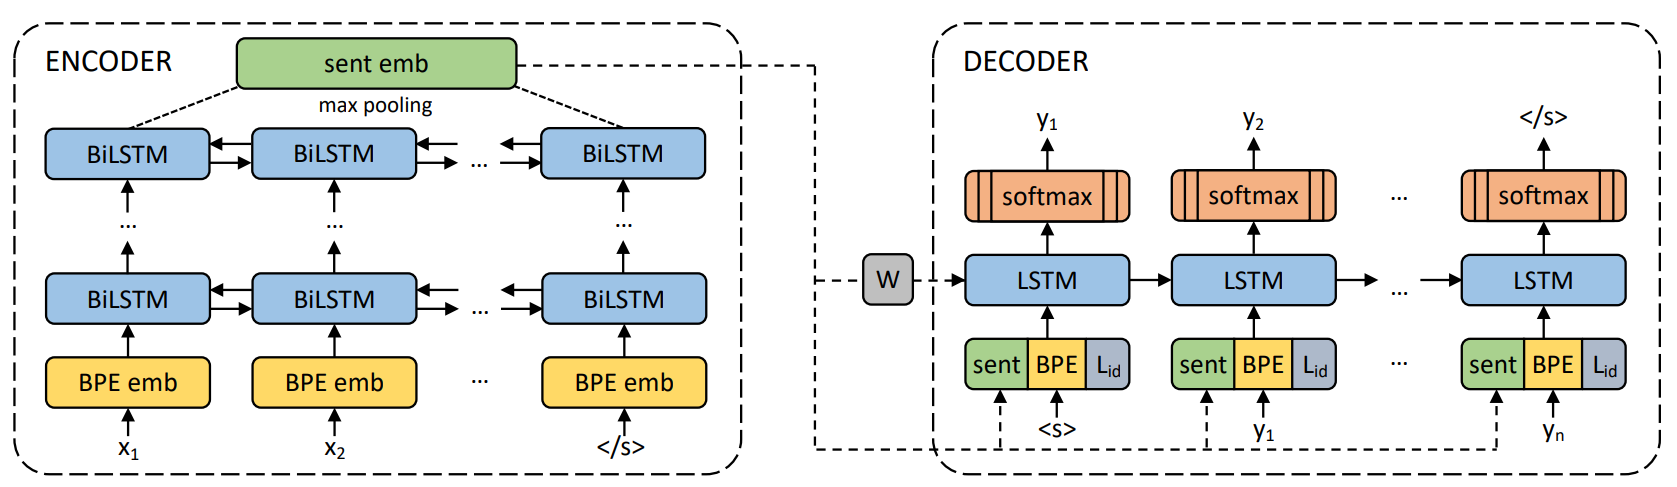
\includegraphics[scale=0.3]{images/laser_architecture}
	\caption[\textit{LASER} encoder architecture]
		{The architecture of the `massively multilingual sentence embeddings' which are part of the \textit{\gls{laser}} library.
		The image was taken from \citep{Artetxe.2018}.}
	\label{fig:laser_architecture}
\end{figure}

The sentence representation is then passed on to the decoder which generates a sequence of words similar to the \textit{Skip-Thought} approach. However, this model additionally gets a language flag as input indicating which language the decoder has to produce. With their approach the authors attempt to create \textbf{`universal language-agnostic sentence representations'}, i.\,e. the embeddings are designed to work well across many tasks and across multiple languages.

% -----------------------------------------------------------------------------------------------------------------------------------------------------
% Random Sentence Encoders
\subsubsection{Random Sentence Encoders}
\label{sec:rand_sent}

Recent research conducted by \citep{Wieting.2019} revealed that \textbf{random sentence representations provide a solid baseline} for more sophisticated algorithms. The authors investigate the results of several models whose parameters are chosen randomly without any training. It was found that while there is a gap between the performance of such random encoders and the representations generated by trained models, it is much smaller than one would expect. Three architectures are proposed in the paper: \ding{182} \textit{\gls{borep}}, \ding{183} \textit{random (Bi-)LSTMs} and \ding{184} \textit{\glspl{esn}} \citep{Jaeger.2001} out of which the first two are used in this thesis.

% -----------------------------------------------------------------------------------------------------------------------------------------------------
% Acquisition of Sentence Embeddings
\subsection{Acquisition of Sentence Embeddings}
\label{sec:sent_embs_acquisition}

Analogously to the previous chapter, it is useful to summarize the training details for all the sentence embeddings considered in the context of the experiments. Table \vref{tab:sent_emb_sources} gives an overview.

\highlight{Non-parameterized methods.} Recall, that non-parameterized methods do not require any training. Instead, they combine existing word embeddings (compositional models). The experiments will be conducted using all word embeddings discussed in section \vref{sec:word_embs} (\textit{word2vec}, \textit{FastText} and \textit{Attract-Repel}). All of these word embedding spaces have a dimensionality of 300 which entails that the sentence embeddings produced by the compositional models have the same dimensionality. An exception is the \textit{power means} embedding which is a concatenation of various means, where $p \in \{ -\infty, 0, 1, 2, +\infty \}$. Furthermore, the code for the \textit{hierarchical pooling} algorithm could not be found in the official repository, which is why it was implemented from scratch according to the paper. In the paper, a window size of $m = 5$ is used. Unfortunately, this information was discovered relatively late which is why the experiments were conducted with a different windows size of $m = 3$.

\highlight{Parameterized methods.} In the context of this thesis five trained parameterized methods are going to be evaluated: \textit{InferSent}, \textit{Quick-Thought}, \textit{sent2vec}, \textit{\gls{bert}} and \textit{\gls{laser}}. Furthermore, there are two types of random encoders: \textit{\gls{borep}} and the \textit{random \gls{bilstm}}. These random methods have parameters (parameterized method), but they are not trained after a random initialization. These models will (next to the majority class) serve as a baseline.

\textbf{Quick-Thought.} The \textit{Quick-Thought} models were trained on the Wikipedia dumps for the respective languages. The English model was also trained on Wikipedia and not downloaded from the official GitHub\github~ repository.\footnote{\url{https://github.com/lajanugen/S2V} (retrieved: September 04, 2019)} The reason for this is that there were some problems when trying to get the pre-trained model to work. Several issues regarding this problem have already been filed.\footnote{Cf. for example \url{https://github.com/lajanugen/S2V/issues/10} or \url{https://github.com/lajanugen/S2V/issues/8} \\ (retrieved: September 17, 2019)} Furthermore, for the Turkish and Georgian models, the number of epochs trained was increased, since there is considerably less data available for these languages.

\textbf{InferSent.} We trained the \textit{InferSent} models on the \gls{snli} data set. Unfortunately, this data set is originally only available for the English language. Therefore, the resources had to be translated. This was achieved using the Google translation \gls{api}. A major problem in this context was that the number of translation requests is limited. Only a certain number of requests per day are allowed. If this limit is exceeded, the server responds with \texttt{Error Code 500: Too many Requests} and one is blocked for 24\,h. In order to increase the speed, several sentences are concatenated which are jointly translated as a batch. Unfortunately, this entails that the translated sentences have to be mapped back to the original sentences (since the result returned is only one long string). It is crucial to assure that the number of sentences returned by the server is equal to the number of sentences fed into the translation procedure. If this is not the case, one risks that sentences and labels do not match anymore which would greatly impair the learning process.

In order to avoid this, the following strategy was employed: A special split token (a series of numbers) was introduced before concatenating the individual sentences in the original language. It was checked that this split token does not influence the quality of the translations in any harmful way. Further, the token was chosen such that it is not altered during the translation procedure (at least in the majority of the cases). When a translated batch arrives it is first split using this split token. The routine subsequently checks if this results in the expected number of sentences. If yes, the sentences are returned. If not, the split token is removed and the next attempt is to split at punctuation symbols (., !, ?). If this again fails, the sentences in that batch are translated one by one. The translations had to be done for Russian, Turkish and Georgian. A German translation of the \gls{snli} data set was already available.\footnote{\url{https://public.ukp.informatik.tu-darmstadt.de/arxiv2018-xling-sentence-embeddings/translated-snli/en-de-translated-snli-4x.zip} (retrieved: September 04, 2019)}

Since the translation procedure nonetheless took a very long time, it was not possible to translate all of the approximately 550,000 sentence pairs for each language, which is why the training set for the low-resource languages was restricted to 60,000 sentence pairs. All models employed use the \textit{InferSent2} version (using \textit{FastText} word embeddings) and the encoder architecture leveraged was the \gls{bilstm} with max-pooling, since this architecture achieved the best results in the experiments conducted by \citep{Conneau.2017}. Training the models takes a very long time. The time for training the German model was about 4 days. The English model was again available for download.\footnote{\url{https://github.com/facebookresearch/InferSent} (retrieved: September 04, 2019)}

% Table: Acquisition of sentence embeddings / models
\begin{table}
	\begin{adjustbox}{angle=90}
		\setlength{\fboxsep}{0pt}
\renewcommand{\arraystretch}{1.415}
\scalebox{1.0}{
\begin{tabularx}{0.935\textheight}{| c | l | p{0.6cm} | c | c | c | c | c | c | X |}
	\hline
	\cellcolor{tud9c!50}													&
	\cellcolor{tud9c!50}													&
	\cellcolor{tud9c!50}													&
	\cellcolor{tud9c!50}													&
	\cellcolor{tud9c!50}													&
	\multicolumn{5}{c |}{\cellcolor{tud9c!50}\textbf{Training details}} 		\\
	\cellcolor{tud9c!50}\multirow{-2}{*}{\textbf{Nr.}}						&
	\cellcolor{tud9c!50}\multirow{-2}{*}{\textbf{Embedding}}				&
	\cellcolor{tud9c!50}\multirow{-2}{*}{\textbf{Lng}}						&
	\cellcolor{tud9c!50}\multirow{-2}{*}{\textbf{Source}}					&
	\cellcolor{tud9c!50}\multirow{-2}{*}{\textbf{Word emb}}				&
	\cellcolor{tud9c!30}\textbf{dim}										&
	\cellcolor{tud9c!30}\textbf{\# instances} 								&
	\cellcolor{tud9c!30}\textbf{batch size} 									&
	\cellcolor{tud9c!30}\textbf{\# epochs} 									&
	\cellcolor{tud9c!30}\textbf{other params / comments}					\\
	\hline\hline
	\multicolumn{10}{| l |}{
		\cellcolor{tud9c!5}\textbf{Non-parameterized methods}}				\\ \hline

	% mean embeddings
	\circled{1} 															&
	\textit{Vanilla average}												&
	\AddCellBackground{0.6cm}{1.1\baselineskip}{images/flag_all}	 		&
	\faFilter																&
	\textit{all} 															&
	300																	&
	-		 															&
 	- 																	&
	- 																	&
	no training required													\\
	\hline

	% p-mean embeddings
	\circled{2} 															&
	\textit{$p$-means}													&
	\AddCellBackground{0.6cm}{1.1\baselineskip}{images/flag_all}	 		&
	\faFilter																&
	\textit{all} 															&
	1,500																	&
	-		 															&
 	- 																	&
	- 																	&
	no training required, $p \in \{ -\infty, 0, 1, 2, +\infty \}$								\\
	\hline

	% sif
	\circled{3} 															&
	\textit{\gls{sif}}														&
	\AddCellBackground{0.6cm}{1.1\baselineskip}{images/flag_all}	 		&
	\faFilter																&
	\textit{all} 															&
	300																	&
	-		 															&
 	- 																	&
	- 																	&
	no training required													\\
	\hline
	
	% gem
	\circled{4} 															&
	\textit{\gls{gem}}													&
	\AddCellBackground{0.6cm}{1.1\baselineskip}{images/flag_all}	 		&
	\faFilter																&
	\textit{all} 															&
	300																	&
	-		 															&
 	- 																	&
	- 																	&
	no training required													\\
	\hline

	% hier. pooling
	\circled{5} 															&
	\textit{hier. pooling}													&
	\AddCellBackground{0.6cm}{1.1\baselineskip}{images/flag_all}	 		&
	\faFilter																&
	\textit{all} 															&
	300																&
	-		 															&
 	- 																	&
	- 																	&
	no training required, window size $m = 3$										\\
	\hline\hline

	\multicolumn{10}{| l |}{
		\cellcolor{tud9c!5}\textbf{Parameterized methods}}					\\
	\hline

	% quickthought
	\circledBlk{1}														&
	\textit{Quick-Thought} 												&
	\AddCellBackground{0.6cm}{1.1\baselineskip}{images/flag_uk}	 		&
	\faCogs																&
	\textit{word2vec}														&
	2,400																&
	97,285,870															&
 	2,000 																&
	5 																	&
	-																	\\
	\hline

	\circledBlk{2}														&
	\textit{Quick-Thought} 												&
	\AddCellBackground{0.6cm}{1.1\baselineskip}{images/flag_germany}		&
	\faCogs																&
	\textit{word2vec} 													&
	2,400																&
	40,729,339 															&
 	1,000 																&
	5 																	&
	-																	\\
	\hline

	\circledBlk{3}														&
	\textit{Quick-Thought} 												&
	\AddCellBackground{0.6cm}{1.1\baselineskip}{images/flag_russia} 		&
	\faCogs																&
	\textit{word2vec} 													&
	2,400																&
	25,324,234		 													&
 	1,000																&
	5 																	&
	-																	\\
	\hline

	\circledBlk{4}														&
	\textit{Quick-Thought} 												&
	\AddCellBackground{0.6cm}{1.1\baselineskip}{images/flag_turkey} 		&
	\faCogs																&
	\textit{word2vec} 													&
	2,400																&
	3,797,955 															&
 	100 																&
	5 																	&
	-																	\\
	\hline

	\circledBlk{5}														&
	\textit{Quick-Thought} 												&
	\AddCellBackground{0.6cm}{1.1\baselineskip}{images/flag_georgia}		&
	\faCogs																&
	\textit{word2vec} 													&
	2,400																&
	1,047,780															&
 	100 																&
	12 																	&
																		\\
	\hline

	% infersent
	\circledBlk{6}														&
	\textit{InferSent} 														&
	\AddCellBackground{0.6cm}{1.1\baselineskip}{images/flag_uk}	 		&
	\faDownload															&
	\textit{FastText}															&
	4,096																&
	-		 															&
 	- 																	&
	- 																	&
	Version: \textit{infersent2}	, max-pooling, model:
	\href{https://dl.fbaipublicfiles.com/infersent/infersent2.pkl}
		{\linkstyle{Link}}													\\
	\hline

	\circledBlk{7}														&
	\textit{InferSent} 														&
	\AddCellBackground{0.6cm}{1.1\baselineskip}{images/flag_germany}		&
	\faCogs																&
	\textit{FastText}														&
	4,096																&
	547,743		 														&
 	64 																	&
	10 																	&
	Version: \textit{infersent2}	, max-pooling								\\
	\hline

	\circledBlk{8}														&
	\textit{InferSent} 														&
	\AddCellBackground{0.6cm}{1.1\baselineskip}{images/flag_russia}		&
	\faCogs																&
	\textit{FastText}														&
	4,096																&
	60,000	 															&
 	64 																	&
	15 																	&
	Version: \textit{infersent2}	, max-pooling								\\
	\hline

	\circledBlk{9}														&
	\textit{InferSent} 														&
	\AddCellBackground{0.6cm}{1.1\baselineskip}{images/flag_turkey} 		&
	\faCogs																&
	\textit{FastText}														&
	4,096																&
	60,000	 															&
 	64 																	&
	15 																	&
	Version: \textit{infersent2}	, max-pooling								\\
	\hline

	\circledBlk{10}														&
	\textit{InferSent} 														&
	\AddCellBackground{0.6cm}{1.1\baselineskip}{images/flag_georgia}		&
	\faCogs																&
	\textit{FastText}														&
	4,096																&
	60,000	 															&
 	64 																	&
	15 																	&
	Version: \textit{infersent2}	, max-pooling								\\
	\hline

	% sent2vec
	\circledBlk{11}														&
	\textit{sent2vec} 														&
	\AddCellBackground{0.6cm}{1.1\baselineskip}{images/flag_uk}	 		&
	\faDownload															&
	\textit{FastText}														&
	700																	&
	-		 															&
 	- 																	&
	- 																	&
	model: \texttt{sent2vec\_wiki\_bigrams},
	\href{https://drive.google.com/file/d/0B6VhzidiLvjSaER5YkJUdWdPWU0/view}
		{\linkstyle{Link}}													\\
	\hline

	\circledBlk{12}														&
	\textit{sent2vec} 														&
	\AddCellBackground{0.6cm}{1.1\baselineskip}{images/flag_germany}		&
	\faCogs																&
	\textit{FastText}														&
	700																	&
	40,729,339		 													&
 	- 																	&
	9 																	&
	\texttt{lr}: 0.2, \texttt{wordNgrams}: 2,
		\texttt{neg}: 10, \texttt{dropoutK}: 4								\\
	\hline

	\circledBlk{13}														&
	\textit{sent2vec} 														&
	\AddCellBackground{0.6cm}{1.1\baselineskip}{images/flag_russia} 		&
	\faCogs																&
	\textit{FastText}														&
	700																	&
	25,324,234		 													&
 	- 																	&
	9 																	&
	\texttt{lr}: 0.2, \texttt{wordNgrams}: 2,
		\texttt{neg}: 10, \texttt{dropoutK}: 4								\\
	\hline

	\circledBlk{14}														&
	\textit{sent2vec} 														&
	\AddCellBackground{0.6cm}{1.1\baselineskip}{images/flag_turkey}		&
	\faCogs																&
	\textit{FastText}														&
	700																	&
	3,797,955		 													&
 	- 																	&
	9 																	&
	\texttt{lr}: 0.2, \texttt{wordNgrams}: 2,
		\texttt{neg}: 10, \texttt{dropoutK}: 4								\\
	\hline

	\circledBlk{15}														&
	\textit{sent2vec} 														&
	\AddCellBackground{0.6cm}{1.1\baselineskip}{images/flag_georgia}		&
	\faCogs																&
	\textit{FastText}														&
	700																	&
	1,047,780		 													&
 	- 																	&
	9 																	&
	\texttt{lr}: 0.2, \texttt{wordNgrams}: 2,
		\texttt{neg}: 10, \texttt{dropoutK}: 4								\\
	\hline

	% bert
	\circledBlk{16}														&
	\textit{\gls{bert}} 													&
	\AddCellBackground{0.6cm}{1.1\baselineskip}{images/flag_all}	 		&
	\faDownload															&
	-																	&
	768																	&
	-		 															&
 	- 																	&
	- 																	&
	multilingual model:
	\href{https://storage.googleapis.com/bert_models/2018_11_23/multi_cased_L-12_H-768_A-12.zip}
		{\linkstyle{Link}}													\\
	\hline

	% laser
	\circledBlk{17}														&
	\textit{\gls{laser}}													&
	\AddCellBackground{0.6cm}{1.1\baselineskip}{images/flag_all}	 		&
	\faDownload															&
	-																	&
	1,024 																&
	-		 															&
 	- 																	&
	- 																	&
	multilingual model:
	\href{https://github.com/facebookresearch/LASER}
	{\linkstyle{Link}}														\\
	\hline

	% random sentence encoder - borep
	\circledBlk{18}														&
	\textit{RandSent \gls{borep}} 											&
	\AddCellBackground{0.6cm}{1.1\baselineskip}{images/flag_all}	 		&
	\faMagic																&
	\textit{FastText}														&
	4,096																&
	-		 															&
 	- 																	&
	- 																	&
	-																	\\
	\hline

	% random sentence encoder - lstm
	\circledBlk{19}														&
	\textit{RandSent \gls{bilstm}} 											&
	\AddCellBackground{0.6cm}{1.1\baselineskip}{images/flag_all}	 		&
	\faMagic																&
	\textit{FastText}														&
	8,192																&
	-		 															&
 	- 																	&
	- 																	&
	-																	\\
	\hline
\end{tabularx}}
	\end{adjustbox}
	\vspace*{-5mm}
	\caption[Sources of sentence embeddings]
		{Overview of sentence embedding acquisition separated by non-parametric and parametric approaches.
		Legend: \faFilter\ Compositional methods, \faDownload\ downloaded models, \faCogs\ trained models,
		\faMagic\ random encoders}
	\label{tab:sent_emb_sources}
\end{table}

\textbf{sent2vec.} The models for the \textit{sent2vec} approach were trained on Wikipedia (German, Russian, Turkish and Georgian). The values for the hyper-parameters can be read off from table \vref{tab:sent_emb_sources}. The training procedure was rather fast. The English model was downloaded using a link from GitHub\github.\footnote{\url{https://github.com/epfml/sent2vec} (retrieved: September 04, 2019)}

\textbf{\gls{bert}.} Training \textit{\gls{bert}} is only possible if one has a \gls{tpu} at one's disposal. This was not the case. But a multilingual model is offered on GitHub\github.\footnote{\url{https://github.com/google-research/bert/blob/master/multilingual.md} (retrieved: September 04, 2019)} The model used is called \texttt{\gls{bert}-Base, Multilingual Cased}. It is applicable to 104 languages and has about 110 million parameters.

\textbf{\gls{laser}.} The model is multilingual and available in pre-trained form. It was downloaded and installed following the instructions on GitHub\github.\footnote{\url{https://github.com/facebookresearch/LASER} (retrieved: September 04, 2019)}

% -----------------------------------------------------------------------------------------------------------------------------------------------------
% Chapter Summary
\subsection{Summary}
\label{sec:sent_embs_summary}

This chapter introduced several sentence embedding algorithms. Generally speaking, there is a distinction between non-parameterized and parameterized sentence embeddings. The first kind of algorithms makes use of word embeddings as a basis and perform some kind of pooling operation in order to obtain a sentence embedding. The more sophisticated parameterized models which are often realized using neural architectures train sentence embeddings from scratch either in an unsupervised or supervised fashion.

The final section then gave insights into the process of sentence embedding acquisition. Models for the English language were mostly found to be publicly accessible in a pre-trained manner and were therefore downloaded from the official websites. Especially models for the low-resource languages Russian, Turkish and Georgian were not available which is why we had to train them from scratch (\textit{sent2vec}, \textit{Quick-Thought} and \textit{InferSent}).

\newpage
% =======================
% Chapter: Probing Tasks
%
% Author: Daniel Wehner
%

% -----------------------------------------------------------------------------------------------------------------------------------------------------
\section{Probing Tasks}
\label{sec:probing_tasks}

% -----------------------------------------------------------------------------------------------------------------------------------------------------
% Chapter Introduction
\subsection{Introduction}
\label{sec:probing_tasks_intro}

Sentence embeddings have become ubiquitous. Despite the abundance of embedding algorithms, several authors \citep[inter alia]{Adi.2017, Zhu.2018,Veldhoen.2016} noticed that the knowledge about which linguistic features are learned by these embeddings is fairly limited. To tackle this problem,  they introduced the first simple evaluation tasks. Later, \citep{Conneau.2018a} made use of these ideas to systematically test sentence representations. The authors were the first to introduce the concept of probing tasks at a larger scale. This chapter provides details about the tasks used in this thesis.

This chapter is organized as follows: Section \vref{sec:probing_tasks_presentation} introduces the probing tasks already used in the literature which are categorized into three different types: Surface tasks, syntactic tasks and semantic tasks. To allow for a sensible assessment of the applicability of the probing tasks in the target languages considered in this thesis (cf. section \vref{sec:probing_tasks_implementability}), it is crucial to understand the grammatical characteristics of each language, which is why the target languages are briefly outlined in section \vref{sec:presentation_languages}. Finally, section \vref{sec:probing_tasks_implementation} supplies information about the probing task selection and further shows how the respective tasks were designed and how training data sets were acquired.

% -----------------------------------------------------------------------------------------------------------------------------------------------------
% Presentation of Probing Tasks
\subsection{Presentation of Probing Tasks}
\label{sec:probing_tasks_presentation}

Probing tasks have become a common tool in the evaluation of sentence embeddings. According to \citep{Conneau.2018a}, \textbf{a probing task is defined to be a \textit{`classification problem that focuses on simple linguistic properties of sentences'}}. Here, the term `linguistic concepts' comprises all interesting properties of sentences which define their structure or meaning. Generally speaking, the evaluation using probing tasks works as follows:

Given an embedding mechanism and a data set which is labeled with the linguistic property of interest, each sentence is first encoded into a vector of fixed length. The resulting vector representations are subsequently fed into a simple classifier, e.\,g. an \gls{mlp} or a logistic regression model. As usual, the error gradients are back-propagated through the network, but \textbf{the weights of the encoding model are frozen and therefore not adjusted during the procedure}. The ultimate test score (e.\,g. accuracy or any other evaluation metric) of the model trained on top of the embeddings can then be considered and indicator of the extent to which the property is encoded in the representations. If the score is high, information about the linguistic property must either implicitly or explicitly be encoded in the vector representations. If the embeddings lack this information, one has to expect a performance score around the chance level (or majority class). Similarly to \citep{Conneau.2018a}, all tasks are in the following categorized into \textbf{surface tasks} (cf. section  \vref{sec:presentation_probing_tasks_surface}), \textbf{syntactic tasks} (cf. section \vref{sec:presentation_probing_tasks_syntactic}) and \textbf{semantic tasks} (cf. section \vref{sec:presentation_probing_tasks_semantic}). \textbf{However, the classification for some tasks can be ambiguous, since they cover syntactic as well as semantic aspects of sentences.} 

% -----------------------------------------------------------------------------------------------------------------------------------------------------
% Surface Information
\subsubsection{Probing Tasks for superficial Information}
\label{sec:presentation_probing_tasks_surface}

Surface information tasks probe sentence embeddings whether or not they retain information which can be read off from the sentences themselves,  \textbf{without requiring any additional knowledge about the language} (e.\,g. grammar, vocabulary, etc.). A review of the literature revealed the following surface probing tasks:

\circledBlk{1} \highlight{Sentence length (\caps{SentLen}).} This task was introduced by \citep{Adi.2017}, its goal is to predict the length of a sentence given its vector representation. Instead of predicting the exact length, the authors introduced a set of bins to simplify the classification task. The following bins were used: $[0; 4]$, $[5; 8]$, $[9; 12]$, $[13; 16]$, $[17; 20]$, $[21; 25]$, $[26; 29]$, $[30; 33]$, $[34; 70]$, $[71;\infty[$. \citep{Conneau.2018a} adopted this task without modifications. A variant of this task is the \caps{LenMismatch} (length mismatch) task introduced by \citep{Naik.2018}. The input to their model consists of two sentence representations and the classifier is tasked with predicting whether the two sentences have equal length or not. This gives a binary classification problem.  

\circledBlk{2} \highlight{Word content (\caps{WC}).} \citep{Adi.2017} were the first to propose this surface probing task. Embeddings are tested if they encode information about individual words in the sentence. The classifier is fed with the sentence representation as well as a word embedding. It has to give a binary answer whether or not the word represented by the word embedding is contained in the sentence. However, this task formulation violates the criteria for probing tasks postulated by \citep{Conneau.2018a} (\textit{`no additional input to the classifiers'}) which is why they rephrased the task: They sampled 1k mid-frequency words from the training corpus and created a data set, where each sentence contains exactly one word from the set of 1k words previously sampled. The task is to predict which one the sentence contains.

\circledBlk{3} \highlight{Word overlap \caps{(WOverlap)}.} Introduced by \citep{Naik.2018}. Given two sentence embeddings, a classifier has to decide whether the sentences have a considerable amount of words in common or not. The authors designed the task as a distraction test, since sentence pairs with little overlap are more likely to be erroneously labeled as \texttt{NEUTRAL} in the \gls{nli} task. Again, this task does not comply to Conneau's cirteria.

% -----------------------------------------------------------------------------------------------------------------------------------------------------
% Syntactic Information
\subsubsection{Probing Tasks for syntactic Information}
\label{sec:presentation_probing_tasks_syntactic}

The following probing tasks involve the syntax of sentences, i.\,e. \textbf{the way how smaller linguistic entities like words or syllables are arranged in order to form more complex constructs like sentences}. Syntax includes for example the order of words which is strict in some languages and more flexible in others.

\circledBlk{4} \highlight{Bi-gram shift (\caps{BiShift}).} Introduced by \citep{Conneau.2018b}. A word bi-gram is a tuple of two consecutive words in a sentence. E.\,g. the word bi-grams of the sentence \textit{`The cat sat on the mat'} are given by \texttt{(The, cat)}, \texttt{(cat, sat)}, \texttt{(sat, on)}, \texttt{(on, the)} and \texttt{(the, mat)}. The main idea of this task is to randomly pick two adjacent words and change their order. A modified version of the sentence could be \textit{`The \underl{sat} \underl{cat} on the mat'} which a probing task classifier should classify as violating legal word orders. A somewhat related task called \caps{WO} (word order) was proposed by \citep{Adi.2017} in which a classifier is given a sentence embedding as well as the word representations of two words $w_1$ and $w_2$. Based on the input, the classifier has to tell, if $w_1$ comes before $w_2$ or vice versa.

\circledBlk{5} \highlight{Subject-verb agreement (\caps{SVAgree}).} For a sentence to be considered grammatical, it is import that subject and verb agree with each other. E.\,g. in the English present tense, an `s' is appended to the verb to denote the third person singular indicative (\textit{`I walk'} vs. \textit{`He walk\textbf{s}'}). \citep{Linzen.2016} originally leveraged the notion of subject-verb agreement while studying the capabilities of \glspl{rnn} to capture long-range dependencies. This idea can be used in our evaluations as well: We purposefully destroy the subject-verb agreement in given sentences and train a classifier to decide whether the sentence is intact or not (an alternative is to test for \textbf{subject-verb distance}). This task requires syntactic knowledge to a large extent and is not at all trivial, since it is very difficult to automatically determine which subject the verb refers to. A major problem in this context pose intervening nouns, so-called \textbf{agreement attractors}, which happen to be close the the verb but are actually not the subject it refers to. \citep{Bock.1991} introduced the term \textbf{agreement attraction error} for situations in which a noun is erroneously considered the subject of a verb. A large variety of other tasks focusing on similar relationships can be designed, e.\,g. \textbf{number agreement}, \textbf{gender agreement} or \textbf{noun-adjective agreement}.

\circledBlk{6} \highlight{Top constituent (\caps{TopConst}).} A sentence can be split recursively into a series of phrase constituents. Consider the example sentence \textit{`John hit the ball'}. The corresponding parse tree is depicted in figure \vref{fig:parse_tree}. The figure shows that the sentence can be decomposed into [[John]\ssc{\textbf{NP}}[[hit]\ssc{\textbf{V}}[[the]\ssc{\textbf{Det}}[ball]\ssc{\textbf{N}}]\ssc{\textbf{NP}}]\ssc{\textbf{VP}}]\ssc{\textbf{S}}. The top constituent in this example is \texttt{NP VP}. \citep{Shi.2016} labeled sentences with their top constituents. For that, they defined 20 classes. 

% Figure: Parse tree
{
% Set the overall layout of the tree
\tikzstyle{level 1}=[level distance=1cm, sibling distance=4cm]
\tikzstyle{level 2}=[level distance=1cm, sibling distance=4cm]

% Define styles for bags and leafs
\tikzstyle{bag}=[circle,draw=black,fill=tud9c!30,text width=2em,text centered]
\tikzstyle{end}=[circle,draw=black,minimum width=3pt,fill,inner sep=0pt]

\begin{figure}[h]
	\centering
	\begin{tikzpicture}[
		scale=0.9,
		every node/.style={scale=0.8},
		sloped
	]
		\node[bag]{\highlight{S}}
    		child{
        		node[bag]{\highlight{NP}}        
        		child {
            	    		node[end,label=below:{\textbf{John}}]{}
            	    		edge from parent
			}
		}
		child{
                	node[bag]{\highlight{VP}}
			child{
				node[bag]{\highlight{V}}
				child{
					node[end,label=below:{\textbf{hit}}]{}
					edge from parent
				}
				edge from parent
			}
			child{
				node[bag]{\highlight{NP}}
				child{
					node[bag]{\highlight{Det}}
					child{
						node[end,label=below:{\textbf{the}}]{}
						edge from parent
					}
					edge from parent
				}
				child{
					node[bag]{\highlight{N}}
					child{
						node[end,label=below:{\textbf{ball}}]{}
						edge from parent
					}
					edge from parent
				}
				edge from parent
			}
                	edge from parent
            	};
        %	edge from parent         
    		%};
	\end{tikzpicture}
	\caption[Simple parse tree of a sentence]{A simple parse tree for the sentence \textit{`John hit the ball'}. Image taken and adapted from: \url{http://www.wikiwand.com/fr/Arbre_syntaxique} (retrieved: September 05, 2019).}
	\label{fig:parse_tree} 	
\end{figure}}

\circledBlk{7} \highlight{Tree depth (\caps{TreeDepth}).} The task introduced by \citep{Conneau.2018b} also involves syntax trees as shown in figure \vref{fig:parse_tree}. In this task the classifier has to predict the length of the longest path (the depth of the tree) from the root note \texttt{S} to the leaves. In the example above the tree depth is equal to 4.

\circledBlk{8} \highlight{Voice (\caps{Voice}).} Many languages offer the \textbf{possibility of exchanging subject and object in a sentence}, e.\,g. \textit{`\underl{The police}\ssc{subj} deals with \underl{the criminal}\ssc{obj}'} vs. \textit{`\underl{The criminal}\ssc{subj} is dealt with by \underl{the police}\ssc{obj}'}. The first sentence is said to be in \textit{active} voice, while the second one in \textit{passive} voice. \citep{Shi.2016} trained a \gls{nmt} system and took the trained encoder to produce sentence representations. These sentence embeddings were classified into either active or passive voice. The trained classifier could detect the correct voice label in 92.8\,\% of the cases. \citep{Krasnowska.2019} pick up this task to test English and Polish sentence embeddings (they call the task \caps{Passive}).

% -----------------------------------------------------------------------------------------------------------------------------------------------------
% Semantic Information
\subsubsection{Probing Tasks for semantic Information}
\label{sec:presentation_probing_tasks_semantic}

Unlike syntactic tasks, their semantic counterparts do not involve the structure of sentences, they rather test sentence representations for \textbf{aspects of meaning or how sentences are interpreted and understood}. The following tasks exist:

\circledBlk{9} \highlight{Replacement tasks.} A large amount of \textit{`replacement tasks'} has been proposed in the literature. In such tasks, specific words are replaced and a classifier has to predict \textbf{whether the sentence is intact or whether it was modified}. These tasks include for example:

\begin{itemize}
	\item \textbf{Antonyms.} \citep{Naik.2018} pick words from the sentence and replace them by antonymous words using \textit{WordNet} \citep{Miller.1995}. 
	\item \textbf{\gls{somo}.} Introduced by \citep{Conneau.2018a}. In this task, a noun or a verb is replaced without destroying the grammaticality of the sentence. Furthermore, Conneau and colleagues ensure that `the bigrams formed by the replacement with the previous and following words in the sentence have frequencies that are comparable with those of the original bigrams.`
	\item Further replacement tasks introduced by \citep{Kim.2019}: \textbf{Articles.} Definite (\textit{`the'}) and indefinite articles (\textit{`a'}, \textit{`an'}) are exchanged. \textbf{Comparative.} Replacement of comparative words like \textit{`better'} or \textit{`worse'}. \textbf{Coordinating conjunctions.} Replacement of conjunctions like \textit{`and'}, \textit{`but'}, \textit{`or'}. \textbf{Prepositions.} Replacement of prepositions by one another. \textbf{Quantification.} Test embeddings for quantifier (words like \textit{`all'}) replacement. \textbf{Spatial expressions.} Replacement of spatial words like \textit{`under'} or \textit{`over'}. \textbf{Wh-words.} Replacement of question words like \textit{`what'}, \textit{`where'} and \textit{`who'}.
\end{itemize}

\circledBlk{10} \highlight{Coordination inversion (\caps{CoordInv}).} \citep{Conneau.2018a} randomly change the order of coordinate clauses. The task is to decide whether or not the clauses are in their original order. An example from their paper is: \textit{`They might be only memories, but I can still feel each one'} vs. \textit{`I can still feel each one, but they might be only memories'}.

\circledBlk{11} \highlight{End of sentence (\caps{EOS}).} Introduced by \citep{Kim.2019}. A classifier is given a sentence representation of two concatenated sentences and an integer index. \textbf{The task is to assess whether the integer number is a valid index to split the two sentences.} Punctuation is removed and all words are transformed to lowercase in order not to give the classifier any additional hints where the two sentences have to be split. The authors present the following example (`//' denotes the splitting point): \cmarkgr\ \textit{`the forehead is gathered in a frown // the mouth is slightly parted to reveal the teeth'} vs. \xmark\ \textit{`the forehead is gathered in a frown the mouth // is slightly parted to reveal the teeth'}

\circledBlk{12} \highlight{Negation (\caps{Neg}).} \citep{Naik.2018} construct sentence pairs comprising the original version and a negated version. The two cases have to be told apart. Linguists refer to this as \textbf{positive or negative polarity}. Some languages have special words which are inserted into the sentence to negate their meaning while others have affixes which are prepended or appended to words. The Turkish language is an instance of the latter case. \citep{Sahin.2019} give an example for this: \textit{`Dün okul-a git-\textbf{me}-di-m.'}\footnote{English translation: \textit{`Yesterday I did not go to school.'}} where the affix \textit{`me'} negates the verb. Embeddings learning such features are considered good features in sentiment analysis.

\circledBlk{13} \highlight{Numerical reasoning (\caps{NumReason}).} \citep{Naik.2018} pick sentences containing numbers, subsequently alter and prefix them with expressions like \textit{`more than'} or \textit{`less than'}. The authors present the following example: The sentence \textit{`Tim has 350 pounds of cement in 100, 50, and 25 pound bags'} is changed to \textit{`Tim has less than 750 pounds of cement in 100, 50, and 25 pound bags'}. It is the job of the classifier to classify the two sentences as related.

\circledBlk{14} \highlight{Semantic role (\caps{SemRole}).} This task provides information about the extent to which semantic roles (entity-event relationships) are captured by sentence embeddings. For the data set, \citep{Ettinger.2016} label sentences with the entity-event relationship contained in them. E.\,g. the sentence \textit{`The dog jumps over the fence'} is labeled with its entity-event relationship \textit{`dog-jump'}.

\circledBlk{15} \highlight{Spelling error (\caps{SpellErr}).} Introduced by \citep{Naik.2018}. This task served as the only noise test in the suite of stress test data sets. The goal of the authors was to show in how far \gls{nli} models are robust with respect to spelling errors in the sentences. The data set consists of error-free as well as erroneous sentences which are labeled accordingly. A very similar task which we thought of is to test sentence embeddings for grammaticality. Sentences are altered in a way such that they are no longer grammatical. A classifier is then trained to distinguish between grammatically correct and incorrect sentences.

\circledBlk{16} \highlight{Subject number/object number (\caps{SubjNum} / \caps{ObjNum}).} The concept of grammatical number is an integral part in most languages. In English and many other languages, grammatical number is represented by \textit{singular} and \textit{plural}. \citep{Conneau.2018a} decided to probe sentence embeddings for this linguistic property. To excel in this task, a classifier has to correctly predict the number of the subject. An alternative is to probe for the \textbf{object number} which works accordingly.

\circledBlk{17} \highlight{Tense (\caps{Tense}).} Introduced by \citep{Conneau.2018a}. Sentences are labeled with the tense of their main verb. Given a vector representation of the sentence, the goal is to predict the correct tense. The task is often restricted to present tense and simple past, since other tenses like future, present perfect or past perfect are \textbf{compound forms} and most tree banks use labels on word level and do not consider larger constructs. Consider the example sentence \textit{`I will do it.'}: Each word in the sentence is labeled separately, rather than labeling the entire compound \textit{`will do'} as future tense.

% -----------------------------------------------------------------------------------------------------------------------------------------------------
% Presentation of the Target languages
\subsection{Presentation of Target Languages}
\label{sec:presentation_languages}

The following sections provide a short introduction into the main grammatical characteristics of the target languages. Basic knowledge about these languages is an essential prerequisite when it comes to the evaluation of the probing tasks with respect to their implementability in the target languages (cf. \vref{sec:probing_tasks_implementability}). Some grammatical concepts which are covered by the tasks presented might not be existent in some of the languages. A presentation of English and German is omitted, the focus is rather on the lower-resource languages which may not be as familiar to the English-speaking reader.

% -----------------------------------------------------------------------------------------------------------------------------------------------------
% Russian Language
\subsubsection{Russian Language -- \foreignlanguage{russian}{русский язык}}
\label{sec:russian_language}

According to \citep{Reuther.2009}, the number of Russian native speakers is estimated to approximately 145 million people. Furthermore, about 80 million people learned Russian as a second language. The Slavic language is written in \textbf{Cyrillic script} (cf. figure \vref{fig:cyrillic} for an example). The script consists of 33 letters and distinguishes between upper and lower case letters.

\begin{figure}[h]
	\begin{verse}
		{\Large Exegi monumentum} \\
		\bigskip
		\begin{otherlanguage*}{russian}
			Я памятник себе воздвиг нерукотворный,		\\
			К нему не заростет народная тропа, 			\\
			Вознесся выше он главою непокорной 		\\
			Александрийского столпа. 			

			\medskip

			Нет, весь я не умру — душа в заветной лире	\\
			Мой прах переживет и тленья убежит — 		\\
			И славен буду я, доколь в подлунном мире 	\\
			Жив будет хоть один пиит.
		\end{otherlanguage*}
	\end{verse}
	\caption[Two stanzas from the poem \textit{`Exegi monumentum'} by Alexander Puschkin]
		{Two stanzas from the poem \textit{`Exegi monumentum'} by Alexander Puschkin. The example was taken from \\
		\url{https://www.russlandjournal.de/russische-literatur/gedichte-von-alexander-puschkin/} \\
		(retrieved: September 06, 2019).}
	\label{fig:cyrillic}
\end{figure}

The Russian language is first of all characterized by \textbf{strong inflection} and is therefore a morphologically rich language: Words are adapted to their grammatical function by adding affixes. Word stems can also change entirely. The concept of grammatical \textbf{gender is existent} in the Russian language (three distinct genders) but there are \textbf{no articles} (neither definite nor indefinite articles). Instead, the gender of a noun has to be read off from the word itself. Nouns are also the group of words which are the most diverse in terms of possible word forms: The case system comprises \textbf{six different cases}: \ding{182} Nominative, \ding{183} genitive, \ding{184} dative, \ding{185} accusative, \ding{186} instrumental and \ding{187} prepositional. Verbs do not have as many forms as e.\,g. in German: There are only \textbf{three tenses} (present, past and future tense) and also the word order is not as strict as it is in the German language. Finally, adjectives have to agree with nouns to which they refer in terms of gender and number.

% -----------------------------------------------------------------------------------------------------------------------------------------------------
% Turkish language
\subsubsection{Turkish Language -- Türkçe}
\label{sec:turkish_language}

\citep{Karakurt.2006} provides an overview of the Turkish language which is also known as Istanbul Turkish in order to distinguish it from other Turkic languages. It is the native language of approximately 65 million people. The Turkish alphabet was introduced 1928 by Mustafa Kemal Atatürk and comprises 29 characters (cf. figure \vref{fig:turkish_script} for an exemplary text). It replaced the previously used Arabic script. The language is characterized by \textbf{extensive usage of agglutination}. Agglutination refers to the grammatical concept of adding several morphemes to words to adjust them according to their grammatical function in the sentence. This way words can become very long and it is even possible to express entire sentences as one word. Consider the following extreme (and artificial) example: \textit{Çekoslovakyalılaştıramadıklarımızdanmışsınızcasına} which means literally: \textit{`In the manner of you being one of those that we apparently couldn't manage to convert to Czechoslovakian'}.\footnote{The example was taken from: \url{https://en.wikipedia.org/wiki/Turkish_language} (retrieved: September 06, 2019).}

% Figure: Turkish example
\begin{figure}[h]
	\begin{verse}
		Orada bir köy var \\
		uzakta \\
		o köy bizim köyümüzdür \\
		gitmesekte \\
		görmesekte \\
		o köy bizim köyümüzdür.
	\end{verse}
	\vspace*{-3mm}
	\caption[Poem written in the Turkish alphabet]{A short poem written in the Turkish alphabet. The example was taken from: \url{http://www.schule-mehrsprachig.at/fileadmin/schule_mehrsprachig/redaktion/sprachensteckbriefe/pdf/ssb_tuerkisch_neu.pdf} (retrieved: September 06, 2019).}
	\label{fig:turkish_script}
\end{figure}

Turkish sentences usually follow the word order \texttt{subject-object-verb} (the verb follows the object, unlike in German). This is the case not only for affirmative clauses but also for interrogative clauses. Furthermore, there is \textbf{no grammatical gender} and \textbf{neither definite nor indefinite articles} are available. The Turkish language is also characterized by a great extent of regularity. There are only a few exceptions to rules. E.\,g. verbs usually follow the standard rules for conjugation (only few irregular verbs exist). Noun declension is diverse: The Turkish language differentiates between \textbf{six cases}: \ding{182}\,Nominative, \ding{183} genitive, \ding{184} dative, \ding{185} accusative, \ding{186} ablative (used to express motion away from something) and \ding{187}\,locative (used to refer to a location). In general, \textbf{adjectives are not declined}, i.\,e. adapted to gender or number.\footnote{Cf. \url{https://www.colanguage.com/turkish-adjectives} (retrieved: October 02, 2019)}

% -----------------------------------------------------------------------------------------------------------------------------------------------------
% Georgian Language
\subsubsection{Georgian Language -- \mxedr{kartuli ena}}
\label{sec:georgian_language}

\citep{Chapidze-Morgenroth.2015} introduces main aspects of the Georgian language.\footnote{Additional information taken from \url{https://deacademic.com/dic.nsf/dewiki/510990}; (retrieved: October 02, 2019)} It is spoken by approximately 4.5 million native speakers and is therefore considered a \textbf{low-resource language} in the \gls{nlp} community.\footnote{A language is said to be low-resource, if there is only little annotated training data available that can be used to train \gls{nlp} systems.} It is a South Caucasian language with its own script called \textbf{Mkhedruli}.\footnote{Derived from the Georgian word \textit{`mkhedari'} which corresponds to the English word \textit{`knight'}.} The alphabet consists of 33 characters (like Cyrillic) each of which corresponds to a phoneme. Furthermore, there is no distinction between capital and non-capital letters. To get a better idea of what the script looks like, figure \vref{fig:mkhedruli} shows the beginning of the Georgian national epos \textit{`The knight in the Tiger's skin'} written in Mkhedruli script. Agglutination as well as inflection are typical of the language. \textbf{It does not possess the concept of grammatical gender} and also (definite and indefinite) \textbf{articles are missing}. Prepositions are replaced by \textbf{postpositions}\footnote{A German example for a postposition would be `den Fluss \textbf{entlang}' (\url{https://de.wikipedia.org/wiki/Georgische_Sprache}; \\ retrieved: September 06, 2019).} and the Georgian \textbf{word order is relatively free}. \citep{Makharoblidze} give an example for this using the sentence \textit{`I am in Tbilisi.'}. The following variants are possible:

\begin{itemize}\setlength\itemsep{-1em}
	\item me var tbilisshi. (I am Tbilisi-in)
	\item me tbilisshi var. (I Tbilisi-in am)
	\item var me tbilishsi. (am I Tbilisi-in)
\end{itemize}

The language developed a comprehensive case system. It has \textbf{seven cases} which are as follows: \ding{182} Nominative, \ding{183}\,ergative, \ding{184} dative, \ding{185} vocative (used to address someone), \ding{186} adverbial (used to mark adverbial phrases), \ding{187} genitive and \ding{188} instrumental (corresponds to the preposition `with' in English: \textit{`He is eating \textbf{with a fork}'}). While most European languages organize verb forms by tenses, modes and aspects, the Georgian language introduces the \textbf{concept of screeves}. There are \textbf{eleven screeves} each of which represents a combination of tense, mode and aspect. A screeve does not only affect the verb but also the form and case of the subject and the object. Equally striking is the high number of irregular verbs in the language.\footnote{For more information cf. \url{https://deacademic.com/dic.nsf/dewiki/510990} (retrieved: October 02, 2019).}

% Figure: Georgian example
\begin{figure}[h]
	\begin{verse}
		{\Large\mxedc ve.pxis .tqaosani} \\
		\medskip
		{\large\mxedc +sota rustaveli} \\
		\bigskip
		\begin{mxedr}
			.gmertsa +semvedre, nutu .kvla damxsnas soplisa +sromasa,		\\
			cecxls, .cqalsa da mi.casa, haerta tana +sromasa;					\\
			momcnes prteni da a.gvprinde, mivhxvde mas +cemsa ndomasa,	\\
			d.gisit da .gamit vhxedvide mzisa elvata .krtomasa.
		
			\medskip
		
			mze u+senod ver ikmdebis, ratgan +sen xar masa .cili,			\\
			gana.gamca mas eaxel misi e.tli, ar tu .cbili!						\\
			muna gnaxo, madve gsaxo, ganminatlo guli +crdili,				\\
			tu sicocxle m.care mkonda, si.kvdilimca mkonda .t.kbili!
		\end{mxedr}
	\end{verse}
	\caption[Two stanzas from \textit{`The knight in the Tiger's Skin'} written in Mkhedruli script]
		{Two stanzas from \textit{`The knight in the Tiger's Skin'} (Georgian national epos) written in Mkhedruli script.
		The example was taken from \url{http://ftp.gwdg.de/pub/ctan/fonts/georgian/mxedruli/mxeddoc.pdf} \\
		(retrieved: September 06, 2019).}
	\label{fig:mkhedruli}
\end{figure}

The following table \vref{tab:presentation_languages} summarizes the main aspects for all languages considered in the context of this thesis:

% Table: Summary of the languages presented
\begin{table}[h]
	\centering
	\renewcommand{\arraystretch}{2.0}
	\scalebox{1.0}{
	\begin{tabular}{| l ? c | c | c | c | c ? l |}
		\hline
		\rowcolor{tud9c!50}
		\textbf{Property}		&
		\textbf{EN} 			&
		\textbf{DE} 			&
		\textbf{RU} 			& 
		\textbf{TR} 			& 
		\textbf{KA} 			&
		\textbf{Comments}	\\
		\hline\hline
		Gender					& 	\cre			&	\cgr			&	\cgr			&	\cre			& 	\cre 		
								& 																				\\
		Articles 					& 	\cgr			& 	\cgr			& 	\cgr			& 	\cre			&	\cre 	
								&																				\\
		Number of cases			& 	\cre			& 	\gry{4}		& 	\gry{6}		& 	\gry{6}		& 	\gry{7}
								& 																				\\
		Number of tenses 		& 	\gry{12}		& 	\gry{6}		& 	\gry{3}		& 	\gry{4}		&	\gry{11}	
								& 	English: + aspect tenses (\textit{-ing}-forms) 									\\
		Lower/Upper case	 letters	&	\cgr			&	\cgr			&	\cgr			&	\cgr			&	\cre 		
								&																				\\
		Script 					&	\gry{L} 		& 	\gry{L} 		& 	\gry{C} 		& 	\gry{L} 		& 	\gry{M} 		
								& 	L: Latin, C: Cyrillic, M: Mkhedruli												\\
		Number of characters		& 	\gry{26}		&	\gry{30}		&	\gry{33}		&	\gry{29}		&	\gry{33}		
								&	German: + \textit{`ä'}, \textit{`ö'}, \textit{`ü'} and \textit{`ß'}					\\
		Inflection/Agglutination 	&	\gry{I} 		& 	\gry{I} 		& 	\gry{I} 		& 	\gry{A} 		& 	\gry{I/A} 	
								&	I: Inflectional, A: Agglutinative													\\
		\hline
	\end{tabular}}
	\caption[Summary of the characteristics of the languages presented]
		{Summary of the characteristics of the languages presented.}
	\label{tab:presentation_languages}
\end{table}

% -----------------------------------------------------------------------------------------------------------------------------------------------------
% Implementability of the Probing Tasks in the Target Languages
\subsection{Implementability of Probing Tasks}
\label{sec:probing_tasks_implementability}

After having introduced the probing tasks as well as the main grammatical aspects of the low-resource target languages (Russian, Turkish and Georgian), we now evaluate the probing tasks with respect to their implementability in the languages considered. As already mentioned, concepts that are available in some languages do not necessarily have to be included in all languages.

One aspect which stands out immediately is that there are \textbf{no definite and indefinite articles} in Russian, Turkish as well as in the Georgian language. As a consequence, the \caps{Article} probing task is not reasonable for these languages. Furthermore, the word order in Russian and Georgian are not as strict which might cause problems in the \caps{WO} task as well as in the \caps{BiShift} task. Nevertheless, these probing tasks are still considered possible candidates for the mentioned languages, since it is assumed that there is still a preferred word order which sounds the `most natural' for native speakers.\footnote{In the overview provided by \citep{Makharoblidze}, the author explains that the basic structure follows \texttt{subject-verb-object}, but deviations are allowed.} One further aspect to keep in mind is that \textbf{the Georgian language does not have tenses as they are known in European languages}. Instead, the language distinguishes between several `screeves' (combinations of tenses, modes and aspects) also known as series which adds more complication. This, too, has to be reflected in the framing of the \caps{Tense} probing task, if this task is chosen for the Georgian language. Finally, there are \textbf{no prepositions in Georgian}. Thus, for a \caps{Preposition} probing task we would have to replace postpositions.

\textbf{Agglutination is another aspect which might cause problems in some tasks.} One task where this could be problematic is the \caps{WC} task. Since words rarely appear in their base form in agglutinative languages, it might be difficult to generate large data sets. In such languages, the way the word is used in the sentence changes the surface form of the word by adding affixes to the word stem. Consider an example from the Turkish language:\footnote{The example was taken from: \url{https://www.grammatiken.de/tuerkische-grammatik/tuerkisch-agglutinierende-sprache-suffix-anhaengen.php} (retrieved: October 11, 2019).} \textit{`evler'} (houses) $\leftrightarrow$ \textit{`evlerim'} (my houses). Whereas in English, the word \textit{`houses'} keeps its surface form, it changes in Turkish.\footnote{Furthermore, both Turkish words would be assigned different word embeddings.}

The following three tables (cf. table \vref{tab:implementability_probing_tasks_sur_syn}, table \vref{tab:implementability_probing_tasks_sem_i} and table \vref{tab:implementability_probing_tasks_sem_ii}) summarize the assessments of the implementability of the probing tasks in the column \texttt{`Applicability'}. Tasks which are applicable to the language without restriction are marked in \cbox{green!30}{\textcolor{green!30!black}{green color}}, tasks which are meaningful in general, but the idiosyncrasies of the language might cause problems in the implementation are marked with \cbox{orange!30}{\textcolor{orange}{orange}} color. If a task is not applicable whatsoever (e.\,g. due to reasons listed above), it is marked in \cbox{red!30}{\textcolor{red}{red}} color.

The other column named \texttt{`Data creation'} provides information about how easy or difficult it is to create appropriate training data for the probing tasks. A \cbox{green!30}{\textcolor{green!30!black}{green}} cell symbolizes that the process of creation is easy and can be automated entirely. This is mainly the case for the tasks which probe sentences for surface information. For them, no additional knowledge about the languages is necessary and the data sets can be created by looking at the surface forms of the sentences alone while the meaning or the syntax of the sentences can be disregarded entirely. An \cbox{orange!30}{\textcolor{orange}{orange}} cell denotes that more linguistic knowledge or special \gls{nlp} tools like taggers or parsers (or tagged data sets and tree banks) are required. Data set creation can be automated to a large extent, if these resources exist, but still, we expect that the implementation entails more problems. A probing task marked with \cbox{red!30}{\textcolor{red}{red}} color is very difficult to implement, since resources probably do not exist or the required linguistic knowledge is not available. For example, the \caps{NumReason} task is (almost?) impossible to implement, if one is not able to speak the corresponding language. Furthermore, a manual creation of the data set is probably inevitable. We believe that if the process is partially automated, it is then at least necessary to conduct a thorough visual inspection, since a computer can easily introduce ungrammatical sentences. Finally, a \cbox{black}{\textcolor{white}{black}} marker refers to the fact that the probing task is not applicable to the language and therefore a sensible data set cannot be created.

The last column called \texttt{`Comments'} leaves room for additional remarks and examples.

% Table: Implementability of probing tasks
\begin{landscape}
	\begin{table}
	\centering
	\renewcommand{\arraystretch}{2.5}
	{\small
		\begin{tabular}{| l | l ? c | c | c | c | c ? c | c | c | c | c ? l |} 
			\hline
			\cellcolor{tud9c!50} 									&
			\cellcolor{tud9c!50}	 								&
			\multicolumn{5}{ c ?}{
				\cellcolor{tud9c!50}\textbf{Applicability}}			&
			\multicolumn{5}{ c ?}{
				\cellcolor{tud9c!50}\textbf{Data creation}}			&
			\cellcolor{tud9c!50}									\\
			\multirow{-2}{*}{
				\cellcolor{tud9c!50}\textbf{Probing task}}			&
			\multirow{-2}{*}{
				\cellcolor{tud9c!50}\textbf{Short description}}		&
			{\cellcolor{tud9c!30}\textbf{EN}} 						&
			{\cellcolor{tud9c!30}\textbf{DE}}						&
			{\cellcolor{tud9c!30}\textbf{RU}} 						&
			{\cellcolor{tud9c!30}\textbf{TR}}						&
			{\cellcolor{tud9c!30}\textbf{KA}}						&
			{\cellcolor{tud9c!30}\textbf{EN}} 						&
			{\cellcolor{tud9c!30}\textbf{DE}} 						&
			{\cellcolor{tud9c!30}\textbf{RU}} 						&
			{\cellcolor{tud9c!30}\textbf{TR}} 						&
			{\cellcolor{tud9c!30}\textbf{KA}}						&
			\multirow{-2}{*}{
				\cellcolor{tud9c!50}\textbf{Comments}}				
			\\ \hline

			% Surface information
			% ==============================================
			\multicolumn{13}{| l |}{
				\cellcolor{tud9c!10}\textit{Probing tasks for \textbf{\underline{\smash{surface}}} information}}	
																\\ \hline\hline
			% Sentence length
			\textbf{Sentence length}								&
			Predict the binned length of a sentence 					&
			\cgr 												&
			\cgr 												&
			\cgr 												&
			\cgr 												&
			\cgr 												&
			\cgr													&
			\cgr													&
			\cgr													&
			\cgr													&
			\cgr													&
																\\ \hline
			% Length mismatch
			\textbf{Length mismatch} 								&
			Test if two sentences have equal length	 				&
			\cgr 												&
			\cgr 												&
			\cgr 												&
			\cgr 												&
			\cgr 												&
			\cgr													&
			\cgr													&
			\cgr													&
			\cgr													&
			\cgr													&
																\\ \hline
			% Word content
			\textbf{Word content}									&
			Decide if a word occurs in the sentence		 			&
			\cgr 												&
			\cgr 												&
			\cgr 												&
			\cgr 												&
			\cgr 												&
			\cgr													&
			\cgr													&
			\cgr													&
			\cor													&
			\cor													&
																\\ \hline
			% Word overlap
			\textbf{Word overlap}									&
			Given two sentences, decide if they overlap 				&
			\cgr 												&
			\cgr 												&
			\cgr 												&
			\cgr 												&
			\cgr 												&
			\cor													&
			\cor													&
			\cor													&
			\cor													&
			\cor													&
			Difficult to define overlap								\\ \hline\hline

			% Syntactic information
			% ==============================================
			\multicolumn{13}{| l |}{
				\cellcolor{tud9c!10}\textit{Probing tasks for \textbf{\underline{\smash{syntactic}}} information}}
																\\ \hline\hline
			% Bi-gram shift
			\textbf{Bi-gram shift}									&
			Predict if sentence has legal word order		 			&
			\cgr 												&
			\cgr 												&
			\cor 												&
			\cgr 												&
			\cor 												&
			\cgr													&
			\cgr													&
			\cgr													&
			\cgr													&
			\cgr													&
			\textit{kids play} vs. \textit{play kids}					\\ \hline
			% Noun pronoun agreement
			\textbf{Noun pronoun agreement}						&
			Check if noun and pronoun agree						&
			\cgr 												&
			\cgr 												&
			\cgr 												&
			\cgr 												&
			\cgr 												&
			\cor													&
			\cor													&
			\cor													&
			\cor													&
			\cor													&
																\\ \hline
			% Subject verb agreement
			\textbf{Subject verb agreement}						&
			Check if subject and verb agree							&
			\cgr 												&
			\cgr 												&
			\cgr 												&
			\cgr 												&
			\cgr 												&
			\cor													&
			\cor													&
			\cor													&
			\cor													&
			\cor													&
			\textit{He goes} vs. \textit{He go}						\\ \hline
			% Top constituent
			\textbf{Top constituent}								&
			Test for top constituency of sentences.					&
			\cgr 												&
			\cgr 												&
			\cgr 												&
			\cgr 												&
			\cgr 												&
			\cor													&
			\cor													&
			\cor													&
			\cor													&
			\cor													&
			\texttt{ADVP NP VP .}									\\ \hline
			% Tree depth
			\textbf{Tree depth} 									&
			Test for hierarchical structure of sentences.				&
			\cgr 												&
			\cgr 												&
			\cgr 												&
			\cgr 												&
			\cgr 												&
			\cor													&
			\cor													&
			\cor													&
			\cor													&
			\cor													&
																\\ \hline
			% Voice
			\textbf{Voice}										&
			Probe for active or passive voice						&
			\cgr 												&
			\cgr 												&
			\cgr 												&
			\cgr 												&
			\cgr 												&
			\cor													&
			\cor													&
			\cor													&
			\cor													&
			\cor													&
			\textit{drive} vs. \textit{is driven}						\\ \hline
			% Word order
			\textbf{Word order} 									&
			Predict if $w_1$ is before $w_2$ or vice versa			&
			\cgr 												&
			\cgr 												&
			\cor 												&
			\cgr 												&
			\cor 												&
			\cgr													&
			\cgr													&
			\cgr													&
			\cgr													&
			\cgr													&
																\\ \hline
		\end{tabular}
		\caption[Overview of the implementability of the surface and syntactic probing tasks in different languages]
				{Overview of the implementability of the surface and syntactic probing tasks in different languages.}
			\label{tab:implementability_probing_tasks_sur_syn}
	}
\end{table}
\end{landscape}

% Table: Implementability of probing tasks
\begin{landscape}
	\begin{table}
	\centering
	\renewcommand{\arraystretch}{2.5}
	{\small
		\begin{tabular}{| l | l ? c | c | c | c | c ? c | c | c | c | c ? l |} 
			\hline
			\cellcolor{tud9c!50} 									&
			\cellcolor{tud9c!50}	 								&
			\multicolumn{5}{ c ?}{
				\cellcolor{tud9c!50}\textbf{Applicability}}			&
			\multicolumn{5}{ c ?}{
				\cellcolor{tud9c!50}\textbf{Data creation}}			&
			\cellcolor{tud9c!50}									\\
			\multirow{-2}{*}{
				\cellcolor{tud9c!50}\textbf{Probing task}}			&
			\multirow{-2}{*}{
				\cellcolor{tud9c!50}\textbf{Short description}}		&
			{\cellcolor{tud9c!30}\textbf{EN}} 						&
			{\cellcolor{tud9c!30}\textbf{DE}}						&
			{\cellcolor{tud9c!30}\textbf{RU}} 						&
			{\cellcolor{tud9c!30}\textbf{TR}}						&
			{\cellcolor{tud9c!30}\textbf{KA}}						&
			{\cellcolor{tud9c!30}\textbf{EN}} 						&
			{\cellcolor{tud9c!30}\textbf{DE}} 						&
			{\cellcolor{tud9c!30}\textbf{RU}} 						&
			{\cellcolor{tud9c!30}\textbf{TR}} 						&
			{\cellcolor{tud9c!30}\textbf{KA}}						&
			\multirow{-2}{*}{
				\cellcolor{tud9c!50}\textbf{Comments}}				
			\\ \hline

			% Semantic information
			% ==============================================
			\multicolumn{13}{| l |}{
				\cellcolor{tud9c!10}\textit{Probing tasks for \textbf{\underline{\smash{semantic}}} information}}
																\\ \hline\hline
			% Antonyms
			\textbf{Antonyms} 									&
			Check if two sentences are antonymous					&
			\cgr 												&
			\cgr 												&
			\cgr 												&
			\cgr 												&
			\cgr 												&
			\cor													&
			\cor													&
			\cor													&
			\cor													&
			\cor													&
																\\ \hline
			% Definite/indefinite articles
			\textbf{Articles} 										&
			Probe if (in-)definite articles were substituted 			&
			\cgr													&
			\cgr													&
			\cre													&
			\cre													&
			\cre													&
			\cgr													&
			\cor													&
			\cgb													&
			\cgb													&
			\cgb													&
			RU, TR, KA: No articles								\\ \hline
%			% Clause relatedness
%			\textbf{Clause relatedness}							&
%			Decide if two sentences are related						&
%			\cgr 												&
%			\cgr 												&
%			\cgr 												&
%			\cgr 												&
%			\cgr 												&
%			\cor													&
%			\cor													&
%			\cor													&
%			\cor													&
%			\cor													&
%			Similar to NLI										\\ \hline
			% Comparative
			\textbf{Comparative}									&
			Probe for comparative replacement						&
			\cgr 												&
			\cgr 												&
			\cgr 												&
			\cgr 												&
			\cgr 												&
			\cor													&
			\cor													&
			\cor													&
			\cor													&
			\cor													&
																\\ \hline
			% Coordinating conjunctions
			\textbf{Coordinating conjunctions} 						&
			Probe for conjunction replacement						&
			\cgr 												&
			\cgr 												&
			\cgr 												&
			\cgr 												&
			\cgr 												&
			\cor													&
			\cor													&
			\cor													&
			\cor													&
			\cor													&
																\\ \hline
			% Coordination inversion
			\textbf{Coordination inversion} 						&
			Predict if coordinate clauses are inverted					&
			\cgr 												&
			\cgr 												&
			\cgr 												&
			\cgr 												&
			\cgr 												&
			\cre													&
			\cre													&
			\cre													&
			\cre													&
			\cre													&
																\\ \hline
			% End-of-Sentence
			\textbf{End of sentence}								&
			Decide where to split two sentences						&
			\cgr 												&
			\cgr 												&
			\cgr 												&
			\cgr 												&
			\cgr 												&
			\cgr													&
			\cgr													&
			\cgr													&
			\cgr													&
			\cgr													&
																\\ \hline
			% Grammaticality
			\textbf{Grammaticality}								&
			Test if sentence is grammatical							&
			\cgr 												&
			\cgr 												&
			\cgr 												&
			\cgr 												&
			\cgr 												&
			\cgr													&
			\cgr													&
			\cgr													&
			\cgr													&
			\cgr													&
																\\ \hline
			% Negation
			\textbf{Negation} 									&
			Test if sentence is negated								&
			\cgr 												&
			\cgr 												&
			\cgr 												&
			\cgr 												&
			\cgr 												&
			\cor													&
			\cor													&
			\cor													&
			\cor													&
			\cor													&				
																\\ \hline
			% Numerical reasoning
			\textbf{Numerical reasoning}							&
			Test if two sentences contain similar quantities			&
			\cgr 												&
			\cgr 												&
			\cgr 												&
			\cgr 												&
			\cgr 												&
			\cre													&
			\cre													&
			\cre													&
			\cre													&
			\cre													&
																\\ \hline
			% Object number
			\textbf{Object number}								&
			Predict the number of the subject						&
			\cgr 												&
			\cgr 												&
			\cgr 												&
			\cgr 												&
			\cgr 												&
			\cor													&
			\cor													&
			\cor													&
			\cor													&
			\cor													&
																\\ \hline
			% Preposition
			\textbf{Preposition}									&
			Probe sentences for preposition replacement				&
			\cgr 												&
			\cgr 												&
			\cgr 												&
			\cgr 												&
			\cor 												&
			\cor													&
			\cor													&
			\cor													&
			\cor													&
			\cor													&
			Postpositions in KA									\\ \hline
			% Quantification
			\textbf{Quantification} 								&
			Test sentence for quantifier replacement					&
			\cgr 												&
			\cgr 												&
			\cgr 												&
			\cgr 												&
			\cgr 												&
			\cor													&
			\cor													&
			\cor													&
			\cor													&
			\cor													&
																\\ \hline
		\end{tabular}
		\caption[Overview of the implementability of the semantic probing tasks in different languages (part 1)]
				{Overview of the implementability of the semantic c probing tasks in different languages (part 1).}
			\label{tab:implementability_probing_tasks_sem_i}
	}
\end{table}
\end{landscape}

% Table: Implementability of probing tasks
\begin{landscape}
	\begin{table}
	\centering
	\renewcommand{\arraystretch}{2.5}
	{\small
		\begin{tabular}{| l | l ? c | c | c | c | c ? c | c | c | c | c ? l |} 
			\hline
			\cellcolor{tud9c!50} 									&
			\cellcolor{tud9c!50}	 								&
			\multicolumn{5}{ c ?}{
				\cellcolor{tud9c!50}\textbf{Applicability}}			&
			\multicolumn{5}{ c ?}{
				\cellcolor{tud9c!50}\textbf{Data creation}}			&
			\cellcolor{tud9c!50}									\\
			\multirow{-2}{*}{
				\cellcolor{tud9c!50}\textbf{Probing task}}			&
			\multirow{-2}{*}{
				\cellcolor{tud9c!50}\textbf{Short description}}		&
			{\cellcolor{tud9c!30}\textbf{EN}} 						&
			{\cellcolor{tud9c!30}\textbf{DE}}						&
			{\cellcolor{tud9c!30}\textbf{RU}} 						&
			{\cellcolor{tud9c!30}\textbf{TR}}						&
			{\cellcolor{tud9c!30}\textbf{KA}}						&
			{\cellcolor{tud9c!30}\textbf{EN}} 						&
			{\cellcolor{tud9c!30}\textbf{DE}} 						&
			{\cellcolor{tud9c!30}\textbf{RU}} 						&
			{\cellcolor{tud9c!30}\textbf{TR}} 						&
			{\cellcolor{tud9c!30}\textbf{KA}}						&
			\multirow{-2}{*}{
				\cellcolor{tud9c!50}\textbf{Comments}}				
			\\ \hline\hline
			
			% Semantic role
			\textbf{Semantic role}									&
			Predict if sentence contains semantic role				&
			\cgr 												&
			\cgr 												&
			\cgr 												&
			\cgr 												&
			\cgr 												&
			\cor													&
			\cor													&
			\cor													&
			\cor													&
			\cor													&
																\\ \hline
			% SOMO
			\textbf{SOMO} 										&
			Replace noun by other noun. Predict if sentence is intact	&
			\cgr 												&
			\cgr 												&
			\cgr 												&
			\cgr 												&
			\cgr 												&
			\cor													&
			\cor													&
			\cor													&
			\cor													&
			\cor													&
																\\ \hline
			% Spatial Expressions
			\textbf{Spatial expressions} 							&
			Test for substitution of spatial words					&
			\cgr 												&
			\cgr 												&
			\cgr 												&
			\cgr 												&
			\cgr 												&
			\cor													&
			\cor													&
			\cor													&
			\cor													&
			\cor													&
			\textit{\textbf{On}/\textbf{Under} desk}				\\ \hline
			% Spelling error
			\textbf{Spelling error} 								&
			Test if sentence contains spelling errors					&
			\cgr 												&
			\cgr 												&
			\cgr 												&
			\cgr 												&
			\cgr 												&
			\cgr													&
			\cgr													&
			\cgr													&
			\cgr													&
			\cgr													&
			\textit{He goes to schol}								\\ \hline
			% Subject number
			\textbf{Subject number} 								&
			Predict the number of the subject						&
			\cgr 												&
			\cgr 												&
			\cgr 												&
			\cgr 												&
			\cgr 												&
			\cor													&
			\cor													&
			\cor													&
			\cor													&
			\cor													&
			\textit{I go} $\rightarrow$ \texttt{singular}				\\ \hline
			% Tense
			\textbf{Tense} 										&
			Predict the tense of the sentence						&
			\cgr 												&
			\cgr 												&
			\cgr 												&
			\cgr 												&
			\cor 												&
			\cor													&
			\cor													&
			\cor													&
			\cor													&
			\cor													&
			KA: screeves											\\ \hline
			% Wh-words
			\textbf{Wh-words}									&
			Decide if a wh-word was replaced						&
			\cgr 												&
			\cgr 												&
			\cgr 												&
			\cgr 												&
			\cgr 												&
			\cor													&
			\cor													&
			\cor													&
			\cor													&
			\cor													&
																\\ \hline
		\end{tabular}
		\caption[Overview of the implementability of the semantic probing tasks in different languages (part 2)]
				{Overview of the implementability of the semantic c probing tasks in different languages (part 2).}
			\label{tab:implementability_probing_tasks_sem_ii}
	}
\end{table}
\end{landscape}

% -----------------------------------------------------------------------------------------------------------------------------------------------------
% Probing Task Selection and Data Set Creation
\subsection{Implementation of Probing Tasks}
\label{sec:probing_tasks_implementation}

The pool of probing tasks already introduced in the literature is vast (cf. section \vref{sec:probing_tasks_presentation} for more details). For reasons of time, it is impossible to implement all of them and as section \vref{sec:probing_tasks_implementability} shows, not all probing tasks are equally suitable for all target languages taken into account in this work. Furthermore, some probing tasks (above all those focusing on semantic aspects) \textbf{require a significant amount of linguistic understanding of the languages}. Unfortunately, this knowledge is quite limited for the low-resource languages like Russian, Turkish or Georgian and the availability of sophisticated \gls{nlp} tools and resources such as taggers, parsers or pre-tagged tree banks might also be restricted to higher-resource languages (or might at least not be available to the same extent in low-resource languages). These circumstances necessitate considering a \textbf{meaningful subset of the probing tasks} for which enough data is available. Furthermore, the set of tasks should probe for interesting linguistic properties in the target languages and should not be too expensive to conduct in terms of time as well as computational cost. Hence, section \vref{sec:selection_corpora} first of all reviews possible corpora which can be used to establish a basis for the data sets. Subsequently, section \vref{sec:probing_tasks_selection} gives some insight into which probing tasks were chosen and lists reasons for their selection.

The next aspect which has to be given adequate thought is how the tasks are set up, \textbf{i.\,e. how each probing task is framed}. Many possibilities are conceivable in this context: A task may be formulated as a classification problem, but also regression would be possible if the target variable was continuous. In this work the focus will be on classification tasks, since there exist no truly continuous output variables.\footnote{However, the length of a sentence can be regarded as a quasi-continuous variable.} The explanations in section \vref{sec:probing_tasks_data_creation} provide detailed information on how the probing data sets were acquired. Ultimately, section \vref{sec:probing_tasks_classifier} presents how the classification algorithm and its architecture was chosen.

% -----------------------------------------------------------------------------------------------------------------------------------------------------
% Selection of Tree Bank Corpora
\subsubsection{Selection of Tree Bank Corpora}
\label{sec:selection_corpora}

The choice of the data source for the purpose of data set creation is essential. First of all, we notice that \textbf{a large number of the probing tasks require knowledge about syntax}. For example in the \caps{SVDist} task it is crucial to know which word plays the role of the subject and which word is considered the predicate of the sentence. While it is easy to determine these parts of a sentence for the English language due to it being spoken by a great majority, it turns out to be quite difficult for languages like Georgian which is not spoken by most people (including the author of the present thesis). Even if one has profound language proficiency, the sheer number of instances a suitable data set requires is prohibitive for manual data creation and labeling, respectively. In general, there are two approaches which are conceivable in order to get hold of the information necessary: \ding{182} The first option is to use an unannotated data set which is processed by leveraging pre-trained taggers and parsers. Unfortunately, especially for the low-resource languages, it is utmost difficult to find such \gls{nlp} tools. \ding{183} A by far more convenient alternative is to acquire a collection of sentences that has already been processed and which is publicly available. Such data sets are called \textbf{tree banks}. We chose the latter approach in the context of this thesis.

Typically, a large amount of tree banks exists, especially for high-resource languages like English or German. All of these could serve as a basis to create probing task data sets. The following list shows the search results for different tree bank corpora in the respective languages:

\begin{tabbing}
	\hspace*{8.5cm}\=\hspace*{1.5cm}\=\kill
	\textbf{Corpus} \> \textbf{Link} \> \textbf{Author/Publication}
	\\[3mm]
	\ding{182} \textbf{English}
	\\[2mm]
	Penn Tree Bank 
		\> 	\href{https://www.kaggle.com/nltkdata/penn-tree-bank/downloads/penn-tree-bank.zip/5}{\linkstyle{Link}}
		\>	\citep{Marcus.1994}
	\\[2mm]
	UD English-EWT {\footnotesize(English web treebank)}		
		\>	\href{https://github.com/UniversalDependencies/UD_English-EWT/tree/master}{\linkstyle{Link}}
		\>	\citep{Silveira.2014}
	\\[2mm]
	UD English-ESL {\footnotesize(English as a second language)}			
		\>	\href{https://github.com/UniversalDependencies/UD_English-ESL}{\linkstyle{Link}}
		\>	\citep{Berzak.2016,Yannakoudakis.2011}
	\\[2mm]
	UD English-LinES {\footnotesize(English-Swedish corpus)}
		\>	\href{https://github.com/UniversalDependencies/UD_English-LinES}{\linkstyle{Link}}
		\>	\citep{Ahrenberg.2007,Ahrenberg.2015}
	\\[2mm]
	UD English-GUM {\footnotesize(Georgetown university multilayer corpus)}
		\>	\href{https://github.com/UniversalDependencies/UD_English-GUM/tree/master}{\linkstyle{Link}}
		\>	\citep{Zeldes.2017}
	\\[2mm]
	UD English-ParTUT {\footnotesize(parallel Turin university treebank)}
		\>	\href{https://github.com/UniversalDependencies/UD_English-ParTUT/tree/master}{\linkstyle{Link}}
		\>	\citep{Sanguinetti.2014a,Sanguinetti.2014b}
	\\[2mm]
	UD English-PUD {\footnotesize(parallel corpus)}
		\>	\href{https://github.com/UniversalDependencies/UD_English-PUD/tree/master}{\linkstyle{Link}}
		\>	\citep{McDonald.2013}
	\\[3mm]
	\ding{183} \textbf{German}
	\\[2mm]
	TIGER
		\> 	\href{https://www.ims.uni-stuttgart.de/forschung/ressourcen/korpora/tiger.html}{\linkstyle{Link}}
		\>	\citep{Brants.2004}
	\\[2mm]
	TüBa-D/Z
		\> 	\href{https://uni-tuebingen.de/de/134290}{\linkstyle{Link}}
		\>	\citep{Hinrichs.2000}
	\\[2mm]
	Hamburg Dependency Treebank
		\> 	\href{https://corpora.uni-hamburg.de/hzsk/de/islandora/object/treebank:hdt}{\linkstyle{Link}}
		\> 	\citep{Foth.2014}
	\\[2mm]
	UD German-GSD
		\> 	\href{https://github.com/UniversalDependencies/UD_German-GSD/tree/master}{\linkstyle{Link}}
		\>	no author found
	\\[2mm]
	UD German-HDT {\footnotesize(Hamburg dependency treebank)}
		\> 	\href{https://github.com/UniversalDependencies/UD_German-HDT/tree/master}{\linkstyle{Link}}
		\>	\citep{Foth.2014}
	\\[2mm]
	UD German-PUD {\footnotesize(parallel corpus)}
		\> 	\href{https://github.com/UniversalDependencies/UD_German-PUD/tree/master}{\linkstyle{Link}}
		\>	\citep{McDonald.2013}
	\\[2mm]
	UD German-LIT {\footnotesize(German literary history)}
		\> 	\href{https://github.com/UniversalDependencies/UD_German-LIT/tree/master}{\linkstyle{Link}}
		\>	no author found
	\\[3mm]
	\ding{184} \textbf{Russian} \>
	\\[2mm]
	UD Russian-GSD
		\> 	\href{https://github.com/UniversalDependencies/UD_Russian-GSD/tree/master}{\linkstyle{Link}}
		\>	no author found
	\\[2mm]
	UD Russian-SynTagRus
		\> 	\href{https://github.com/UniversalDependencies/UD_Russian-SynTagRus/tree/master}{\linkstyle{Link}}
		\>	\citep{Droganova.2018}
	\\[2mm]
	UD Russian-Taiga
		\> 	\href{https://github.com/UniversalDependencies/UD_Russian-Taiga/tree/master}{\linkstyle{Link}}
		\>	\citep{Shavrina.2017}
	\\[2mm]
	UD Russian-PUD {\footnotesize(parallel corpus)}
		\> 	\href{https://github.com/UniversalDependencies/UD_Russian-PUD/tree/master}{\linkstyle{Link}}
		\>	\citep{McDonald.2013}
	\\[3mm]
	\ding{185} \textbf{Turkish}
	\\[2mm]
	UD Turkish-GB {\footnotesize(grammar book corpus)}
		\> 	\href{https://github.com/UniversalDependencies/UD_Turkish-GB}{\linkstyle{Link}}
		\>	\citep{Coltekin.2017}
	\\[2mm]
	UD Turkish-IMST {\footnotesize(ITU-METU-Sabancı treebank)}
		\>	\href{https://github.com/UniversalDependencies/UD_Turkish-IMST}{\linkstyle{Link}}
		\>	\citep{Sulubacak.2016}
	\\[2mm]
	UD Turkish-PUD {\footnotesize(parallel corpus)}
		\>	\href{https://github.com/UniversalDependencies/UD_Turkish-PUD}{\linkstyle{Link}}
		\>	\citep{McDonald.2013}
	\\[3mm]
	\ding{186} \textbf{Georgian}
	\\[0.5mm]
	GNC (Georgian National Corpus)
		\> 	\href{http://gnc.gov.ge/gnc/page}{\linkstyle{Link}}; not publicly available
		\>	
	\\[2mm]
	Universal Dependencies
		\> 	announced, but not yet available
		\>
\end{tabbing}

\highlight{English.} One of the oldest and most prominent tree banks for the English language is the \textit{Penn tree bank} corpus which was created in the period of 1989 to 1996. The corpus contains millions of annotated words (\gls{pos}-tagged, constituency parses, etc.) extracted form a diverse range of sources: E.\,g. news, manuals or transcribed conversations among many more \citep{Taylor.2003}. Another treebank corpus which is well-established in the \gls{nlp} community is the \textit{\gls{ud} tree bank}. It is actually not only one corpus, but a set of diverse corpora from many sources. \textit{\gls{ud}} is an initiative aiming at providing a consistent tagging scheme across many modern languages. According to the website, the project currently comprises approximately 100 treebanks in more than 70 languages.\footnote{\url{https://universaldependencies.org/} (retrieved: September 07, 2019)} And the number of supported languages increases steadily.

\highlight{German.} Many resources exist for the German language. Next to \textit{\gls{ud}} tree banks, other data sets including \textit{TIGER} and \textit{TüBa-D/Z} are available. According to the official website\footnote{\url{https://www.ims.uni-stuttgart.de/forschung/ressourcen/korpora/tiger.html} (retrieved: September 07, 2019)} the \textit{TIGER} corpus comprises approximately 50k sentences extracted from German newspapers which were semi-automatically tagged. The corpus can be downloaded in two different formats: \textit{NeGra} format and \textit{Tiger \gls{xml}}. The \textit{TüBa-D/Z} corpus provided by the University of Tübingen, on the other hand, contains around 105k manually annotated sentences again taken from German newspapers.\footnote{\url{https://uni-tuebingen.de/de/134290} (retrieved: September 09, 2019)} Unfortunately, this corpus cannot be downloaded without registration and is therefore not publicly available. One of the largest tree banks existing for German is the \textit{Hamburg dependency treebank} containing approximately 260k sentences.\footnote{\url{https://corpora.uni-hamburg.de/hzsk/de/islandora/object/treebank:hdt} (retrieved: September 07, 2019)} As a data source the authors used the famous German website \url{heise.de}. This tree bank corpus is also available as a \textit{\gls{ud}} corpus but was  reduced in size.

\highlight{Low-resource languages.} As expected, it turns out to be \textbf{more difficult to locate sets of tagged sentences for the low-resource languages Russian, Turkish and Georgian}. Luckily, there are \textit{\gls{ud}} corpora for all these languages, except for Georgian (which has already been announced on the official \textit{\gls{ud}} website\footnote{\url{https://universaldependencies.org/}, cf. section \textit{`Upcoming UD Languages'} (retrieved: September 07, 2019)}). All \textit{\gls{ud}} tree banks are in general very appealing and \textbf{exhibit the same structure} which is why parsing the corpora for all languages is connected with less effort and other tree banks are often not publicly accessible or registration is required when using them. Since the \textit{\gls{ud}} corpora are furthermore \textbf{drawn from a multitude of domains} (e.\,g. news, literature, web texts, etc.) they are \textbf{representative of the different styles and aspects of each language}. Therefore, the tree banks released by \textit{\gls{ud}} are going to be used as a basis for the creation of probing task data sets. The following figure \vref{fig:ud_example} depicts the general structure of the \textit{\gls{ud}} corpora:

\vspace*{1mm}
\begin{figure}[h]
\scriptsize
\begin{tabbing}
\hspace*{0.5cm}\=\hspace*{1.5cm}\=\hspace*{1.5cm}\=\hspace*{1.5cm}\=\hspace*{1cm}\=\hspace*{5cm}\=\hspace*{0.75cm}\=\hspace*{1.5cm}\=\hspace*{2cm}\=\hspace*{2cm}\=\kill
\texttt{\# sent\_id = weblog-juancole.com\_juancole\_20051126063000\_ENG\_20051126\_063000-0029} 	\\[1mm]
\texttt{\# text = But in my view it is highly significant.} 													\\[2mm]
1	\>	But			\>	but			\>	\texttt{CCONJ}	\>	\texttt{CC}		\>	\_													\>	8			\> 	\texttt{cc}			\>	\texttt{8:cc}				\>	\_ 						\\[1mm]
2	\>	in 			\>	in			\>	\texttt{ADP} 		\>	\texttt{IN} 		\>	\_													\>	4			\>	\texttt{case}			\>	\texttt{4:case}			\>	\_ 						\\[1mm]
3	\>	my			\>	my			\>	\texttt{PRON}	\>	\texttt{PRP\$}	\>	\texttt{Number=Sing|Person=1|Poss=Yes|...}			\>	4			\>	\texttt{nmod:poss}	\>	\texttt{4:nmod:poss}		\>	\_ 						\\[1mm]
4	\>	view		\>	view 		\>	\texttt{NOUN	}	\>	\texttt{NN}		\>	\texttt{Number=Sing}									\>	8			\> 	\texttt{obl}			\>	\texttt{8:obl:in}			\>	\_ 						\\[1mm]
5	\>	it 			\>	it			\> 	\texttt{PRON}	\>	\texttt{PRP}		\> 	\texttt{Case=Nom|Gender=Neut|Number=Sing|...}		\>	8			\>	\texttt{nsubj}		\>	\texttt{8:nsubj}			\>	\_ 						\\[1mm]
6	\>	is			\>	be			\> 	\texttt{AUX} 		\>	\texttt{VBZ}		\>	\texttt{Mood=Ind|Number=Sing|Person=3|...}			\>	8			\>	\texttt{cop}			\>	\texttt{8:cop}			\>	\_ 						\\[1mm]
7	\>	highly		\>	highly		\> 	\texttt{ADV}		\>	\texttt{RB}		\>	\_													\>	8			\>	\texttt{advmod}		\>	\texttt{8:advmod}		\>	\_ 						\\[1mm]
8	\>	significant 	\>	significant	\> 	\texttt{ADJ}		\>	\texttt{JJ}		\>	\texttt{Degree=Pos}									\>	0			\>	\texttt{root}			\>	\texttt{0:root	}			\>	\texttt{SpaceAfter=No}	\\[1mm]
9	\>	.			\>	.			\> 	\texttt{PUNCT}	\>	\texttt{.}			\>	\_													\>	8			\>	\texttt{punct}		\>	\texttt{8:punct}			\>	\_						\\[2mm]
	\>	\ding{182}	\>	\ding{183}	\>	\ding{184}		\>	\ding{185}		\>	\ding{186}											\>	\ding{187} 	\> 	\ding{188}			\>	\ding{189}				\>	\ding{190}
\end{tabbing}
\vspace*{-5mm}
\caption[Exemplary sentence taken from the Universal Dependencies English-EWT corpus]
	{Exemplary sentence taken from the Universal Dependencies English-EWT corpus.}
\label{fig:ud_example}
\end{figure}

Columns \ding{182} and \ding{183} contain the original words and their lemmas, respectively. Columns \ding{184} and \ding{185} contain \gls{pos} tags using two different tag sets. Very important for the creation of the data sets is the information which is listed in column \ding{186}. These are \textbf{morpho-syntactic annotations} of the words. These annotations give information about cases, tenses, moods, numbers, etc. Finally, the dependency annotations are given in columns \ding{187}, \ding{188} and \ding{189} where the number in column \ding{187} is a reference pointer to the regent of the word. Column \ding{188} on the other hand specifies the type of relationship between regent and dependent. 

% Table: Treebank statistics
Often, there are several smaller \textit{\gls{ud}} corpora available (like English-EWT, English-ESL, English-LinEs). In order to get the maximum number of sentences, \textbf{all \textit{\gls{ud}} corpora which could be found for one language were concatenated} (also combining the respective \texttt{train}, \texttt{dev} and \texttt{test} portions). For Georgian, an alternative corpus had to be acquired since the language is not yet officially supported by \textit{\gls{ud}}. The \textit{\gls{gnc}} is in general not publicly accessible, but was made available by courtesy of Mr. Paul Meurer from the University of Bergen (\url{Paul.Meurer@uib.no}) who is one of the researchers involved in the development and maintenance of this corpus. Unfortunately, the \texttt{.zip} file could not be read entirely which is why some sentences are missing. The corpus home page\footnote{\url{http://gnc.gov.ge/gnc/page} (retrieved: September 07, 2019)} gives more information about the project. It is stated that the corpus is still under construction and it contains texts from Old Georgian, Middle Georgian as well as the modern Georgian language. Also transcriptions of spoken language are included into the corpus. Table \vref{tab:treebank_stats} summarizes the number of sentences contained in each corpus. Surprisingly, the Georgian corpus is significantly larger compared to the \textit{\gls{ud}} corpora for the other languages.

% Table: Treebank statistics
\begin{table}[H]
	\centering
	\renewcommand{\arraystretch}{1.2}
	\scalebox{0.95}{
	\begin{tabular}{| c | r |}
		\hline
		\rowcolor{tud9c!50}
		\textbf{Corpus}	&
		\textbf{\# sentences} \\
		\hline\hline
		\textbf{\textit{UD} English} 		& 	32,004	\\
		\textbf{\textit{UD} German} 		& 	188,517	\\
		\textbf{\textit{UD} Russian} 		& 	68,100	\\
		\textbf{\textit{UD} Turkish} 		& 	8,513	\\
		\textbf{\textit{GNC} Georgian} 	& 	990,669	\\
		\hline
	\end{tabular}}
	\caption[Number of sentences contained in the tree banks for each language]
		{Number of sentences contained in the tree banks for each language.}
	\label{tab:treebank_stats}
\end{table}
\vspace*{-5mm}

In some cases it can happen that the sentences from \textit{\gls{ud}} are not sufficient to build probing sets of adequate size. This is especially critical for the Turkish language where only around 8.5k sentences are available from \textit{\gls{ud}}, even after concatenation of all available corpora and split portions. Additionally, we notice that not all probing tasks rely on the availability of annotated tree banks (e.\,g. the \caps{SentLen} task). A lack of data for such probing tasks was tackled by additionally adding sentences from Wikipedia (cf. table \vref{tab:wikipedia_stats}). This step can be considered critical, since some of the sentence encoder architectures were trained on Wikipedia, but it was necessary due to sparsity of data in low-resource languages. \textbf{Attempts to minimize biases were made by resorting to Wikipedia sentences only when absolutely necessary.}

% -----------------------------------------------------------------------------------------------------------------------------------------------------
% Selection of Probing Tasks
\subsubsection{Selection of Probing Tasks}
\label{sec:probing_tasks_selection}

The choice for the implementation of specific probing tasks was mainly dominated by the availability of the information needed to produce the respective data sets. First of all, all surface probing tasks except for \caps{LenMismatch} and \caps{WOverlap} could be implemented. We did not implement \caps{LenMismatch}, since the probing task objective is similar to the \caps{SentLen} task. Furthermore, the task requires two sentences to be fed into the classifier which violates the criteria for probing tasks introduced by \citep{Conneau.2018a}. The latter argument is also the reason why implementing the \caps{WOverlap} task was avoided. \textbf{In general, all probing tasks implemented in the context of the present thesis adhere to the criteria introduced by Conneau and colleagues.}

It was possible to implement the majority of syntactic probing tasks. The \caps{NPAgree} (noun-pronoun agreement) task was not implemented due to several reasons: The first reason is that the kind of information it probes is very similar to the \caps{SVAgree} task. Also, \textbf{noun-pronoun relationships often exist beyond sentence boundaries}, since it is considered better linguistic style to prevent multiple mentions of the same object (E.\,g. \textit{`The house fell victim to the flames. [\st{The house}] $\rightarrow$ \textbf{It} was built in 1836.'}). What is more, the information which pronoun belongs to which noun is \textbf{not included} in the underlying corpus which prevents the creation of high-quality data sets. Finally, the \caps{TopConst} task was excluded, since it turned out to be \textbf{extremely difficult to parse enough data such that reasonably balanced data sets could be produced}. The diversity of the sentences in the corpora is so large that an insufficient amount of parses with identical top constituents are the consequence. For Georgian, Mr. Paul Meurer could supply some constituency parses, but the number of instances only amounts to approximately 40. This is considered to be too less data such that an interpretation of the results is meaningless.

The implementation of semantic probing tasks is the most challenging. All replacement tasks necessitate the compilation of lists for all languages containing words which can be used as a substitute. For example the antonyms task would require lists of adjective-pairs where both elements have antonymous meanings (unfortunately, the authors of \textit{Attract-Repel} did not open source their linguistic constraints data sets which could be used for that). The lists need to be created manually, since tools like WordNet are not available for all the target languages and presumably, the size of these lists would have to be very large in order for the probing data set to contain a sufficient amount of training data. \textbf{This is why such probing tasks were mostly neglected in the context of this thesis.} Instead, we decided to introduce an entirely new task called \caps{SVDist} (subject-verb distance). This task is inspired by the \caps{SVAgree} task, but instead of predicting whether subject and verb agree, the task is to predict the number of tokens between those two sentence elements. Furthermore, the \caps{ObjNum} task is similar to the \caps{SubjNum} task. It is easier to implement the latter one, since the subject is directly annotated in the \textit{\gls{ud}} corpora, while there are several types of objects for which no dedicated labels exist. Thus, the decision fell on the \caps{SubjNum} task. Tasks like \caps{NumReason} or \caps{CoordInv} are very complicated to implement, since they require more than just simple modification operations (like flipping the order of two words). As the necessary knowledge about the lower-resource languages is not available and in order to avoid producing low-quality data sets, we chose not to implement these two tasks and restrict the implementations to tasks for which better quality can be assured. Finally, the \caps{Tense} task would be straightforward to implement, unfortunately the corpora partially contain past tense sentences only which renders a classification pointless. \textbf{Summarizing the above explanations, the following probing tasks were chosen to be implemented:}

\begin{itemize}\setlength\itemsep{0.75em}
\item \parbox[c][1cm][c]{5.5cm}{Implemented \textbf{surface} probing tasks}
	\(
  	\left[ \qquad
    		\begin{minipage}[c]{0.6\linewidth}
    			\item Sentence length (\caps{SentLen})
			\item Word content (\caps{WC})
    		\end{minipage}
  	\right.
  	\)
\item \parbox[c][1cm][c]{5.5cm}{Implemented \textbf{syntactic} probing tasks}
  	\(
  	\left[ \qquad
    		\begin{minipage}[c]{0.6\linewidth}
    			\item Bi-gram shift (\caps{BiShift})
			\item Subject-verb agreement (\caps{SVAgree}) \highlight{$\longrightarrow$ new!}
			\item Subject-verb distance (\caps{SVDist}) \highlight{$\longrightarrow$ new!} \\
				\textbf{\textit{(not implemented for Georgian)}}
			%\item Top constituent \textbf{\textit{(Not implemented for RU and TR)}}
			\item Voice (\caps{Voice})
			\item Word order (\caps{WO})
    		\end{minipage}
  	\right.
  	\)
\item \parbox[c][1cm][c]{5.5cm}{Implemented \textbf{semantic} probing tasks}
	\(
  	\left[ \qquad
    		\begin{minipage}[c]{0.6\linewidth}
    			\item End of sentence (\caps{EOS})
			\item Subject number (\caps{SubjNum})
			%\item Tense
    		\end{minipage}
  	\right.
  	\)
\end{itemize}

% -----------------------------------------------------------------------------------------------------------------------------------------------------
% Creation of Data Sets for the Probing Tasks
\subsubsection{Creation of Probing Task Data Sets}
\label{sec:probing_tasks_data_creation}

\highlight{\caps{SentLen}.} Following \citep{Adi.2017}, we grouped the sentences in bins according to the number of words. The bins were chosen as following: $[1;4], [5;8], [9;12], [13;16], [17;20], [21;25], [26;29], [30;33], [34;55], [56;\infty[$. As an alternative, it is conceivable to predict the sentence length directly. However, the prediction of the exact length would be too demanding and furthermore, very long or short sentences tend to be rare such that the corresponding classes would be underrepresented in the training data set. This can be mitigated by aggregating these rare cases into a single larger class. As can be seen in figure \vref{fig:sent_len_class_distribution}, there is still an imbalance between the classes, but it is less severe due to the binning procedure. Furthermore, the figure reveals that German sentences tend to be longer on average compared to the remaining languages.\footnote{Due to agglutination it is not surprising that Turkish sentences are shorter on average since a single word contains much more information.}

% Figure: Class distribution sentence length
\begin{figure}[h]
	\begin{tikzpicture}
		\begin{axis}[
			ybar,
			x tick label style={/pgf/number format/1000 sep=},
			ylabel=Number of instances,
			enlargelimits=0.15,
			bar width=4pt,
			legend style={at={(0.5,-0.15)},anchor=north,legend columns=-1,/tikz/every even column/.append style={column sep=0.5cm}},
			grid=both,
    			grid style={line width=.1pt, draw=gray!10},
    			major grid style={line width=.2pt,draw=gray!50},
			x=35,
			title=\textbf{Sentence length}
		]

			\addplot coordinates {(0, 0.043) (1, 0.159) (2, 0.179) (3, 0.155) (4, 0.135)
				(5, 0.126) (6, 0.067) (7, 0.046) (8, 0.082) (9, 0.009)};
			\addplot coordinates {(0, 0.006) (1, 0.104) (2, 0.196) (3, 0.199) (4, 0.160)
				(5, 0.145) (6, 0.072) (7, 0.044) (8, 0.066) (9, 0.006)};
			\addplot coordinates {(0, 0.032) (1, 0.167) (2, 0.174) (3, 0.167) (4, 0.143)
				(5, 0.124) (6, 0.068) (7, 0.045) (8, 0.074) (9, 0.005)};
			\addplot coordinates {(0, 0.094) (1, 0.373) (2, 0.189) (3, 0.116) (4, 0.088)
				(5, 0.067) (6, 0.031) (7, 0.016) (8, 0.025) (9, 0.001)};
			\addplot coordinates {(0, 0.071) (1, 0.283) (2, 0.223) (3, 0.148) (4, 0.096)
				(5, 0.019) (6, 0.126) (7, 0.021) (8, 0.048) (9, 0.012)};
            		\legend{English, German, Russian, Turkish, Georgian}

		\end{axis}
	\end{tikzpicture}
	\caption[Sentence distribution by the number of words]{The bar plots depict the sentence distribution by the number of words. As can be seen in the visualization, short to medium-sized sentences (bins 1, 2 and 3) form the majority across all languages. German sentences tend to be longer on average compared to the other languages considered.}
	\label{fig:sent_len_class_distribution}
\end{figure}

% Table: Class distribution sentence length
\begin{figure}[h]
	\begin{tikzpicture}
		\begin{axis}[
			ybar,
			x tick label style={/pgf/number format/1000 sep=},
			ylabel=Number of instances,
			enlargelimits=0.15,
			bar width=4pt,
			legend style={at={(0.5,-0.15)},anchor=north,legend columns=-1,/tikz/every even column/.append style={column sep=0.5cm}},
			grid=both,
    			grid style={line width=.1pt, draw=gray!10},
    			major grid style={line width=.2pt,draw=gray!50},
			x=35,
			title=\textbf{Sentence length}
		]

			\addplot coordinates {(0, 0.043) (1, 0.159) (2, 0.179) (3, 0.155) (4, 0.135)
				(5, 0.126) (6, 0.067) (7, 0.046) (8, 0.082) (9, 0.009)};
			\addplot coordinates {(0, 0.006) (1, 0.104) (2, 0.196) (3, 0.199) (4, 0.160)
				(5, 0.145) (6, 0.072) (7, 0.044) (8, 0.066) (9, 0.006)};
			\addplot coordinates {(0, 0.032) (1, 0.167) (2, 0.174) (3, 0.167) (4, 0.143)
				(5, 0.124) (6, 0.068) (7, 0.045) (8, 0.074) (9, 0.005)};
			\addplot coordinates {(0, 0.094) (1, 0.373) (2, 0.189) (3, 0.116) (4, 0.088)
				(5, 0.067) (6, 0.031) (7, 0.016) (8, 0.025) (9, 0.001)};
			\addplot coordinates {(0, 0.071) (1, 0.283) (2, 0.223) (3, 0.148) (4, 0.096)
				(5, 0.019) (6, 0.126) (7, 0.021) (8, 0.048) (9, 0.012)};
            		\legend{English, German, Russian, Turkish, Georgian}

		\end{axis}
	\end{tikzpicture}
	\caption[Sentence distribution by the number of words]{The bar plots depict the sentence distribution by the number of words. As can be seen in the visualization, short to medium-sized sentences (bins 1, 2 and 3) form the majority across all languages. German sentences tend to be longer on average compared to the other languages considered.}
	\label{fig:sent_len_class_distribution}
\end{figure}

\highlight{\caps{WC}.} Since the task setup introduced by \citep{Adi.2017} pollutes the evaluation by introducing additional input to the classifier, we chose to follow the approach of \citep{Conneau.2018a}. For this task \textbf{it is very important to guarantee that only exactly one word from the list is contained in the sentence}. Otherwise the classification task becomes unfair because one sentence would belong to several classes, thus rendering the class label ambiguous. This circumstance could lead to correct classifications being regarded as misclassifications. Furthermore, due to the binary setup, Adi and colleagues have to construct negative examples, i.\,e. sentences labeled with an arbitrary word not contained in the respective sentences. The necessity of negative examples is avoided by Conneau's setting.

For the implementation we proceeded as follows: First of all, \textbf{instead of sampling 1k words from the corpus, a smaller set of 30 words was picked, because collecting enough training data to distinguish between 1k classes was found to be impossible for the low-resource languages.} As mentioned above, it is crucial that one and only one word from the list is contained in the sentence. In order to facilitate the data generation process, it was therefore necessary to pick words which tend to appear only once in a sentence. Simultaneously their usage must not be that infrequent such that they do appear in sufficiently many sentences. We restricted the choice of words to \textbf{30 mid-frequency nouns}.\footnote{For the identification of nouns the information contained in column \ding{185} of the training corpus was used (cf. figure \vref{fig:ud_example}).} This approach rules out frequently occurring stop words like articles and prepositions which have a tendency to occur more than once in a single sentence. Furthermore, nouns usually appear only once in a sentence, since they are often replaced by pronouns if one wants to refer to them multiple times. Table \vref{tab:wc_words} in the appendix gives an overview of the nouns selected for each language.

\highlight{\caps{BiShift}.} This task probes sentences for legal word orders, where sentences are purposefully manipulated to destroy the legal word order. \textbf{We included each sentence twice in the training data set:} The first variant is the original sentence with the correct order of words. The second one is an altered version, where we intentionally switched the order of a word bi-gram. Sentences are mutilated by first splitting the sentence into a series of tokens using the \gls{nltk} library -- a Python package introduced by \citep{Bird.2002} -- followed by randomly sampling a word form the sentence and subsequently \textbf{switching the position with its right neighbor}. The original sentences are labeled with the positive class (\texttt{class 1}), whereas the other half of the sentences belongs to the negative class (\texttt{class 0}). Furthermore, `sentences' in the underlying corpus which comprise less than 2 tokens (which occurs rarely) are omitted.

\highlight{\caps{SVAgree}.} Probing for the agreement of subject and verb in a sentence requires to construct sentences for which this agreement is broken. We implemented the task as a \textbf{binary classification task}, where \texttt{class 0} denotes disagreement, while \texttt{class 1} represents agreement. The data set was acquired as follows: For each language, we created a list of frequently occurring verbs together with their corresponding present tense conjugations. We checked each individual sentence for the presence of a verb form contained in the list. If no word is present, we excluded the sentence from the probing task data set. \textbf{Otherwise, we randomly replace the verb form by a different conjugation in 50\,\% of the cases.}

The advantage of this approach is obvious: \textbf{It does not require annotated corpora and as a consequence larger training sets can be created.} Yet, there are some pitfalls which have to be dealt with in order to acquire high-quality data: \ding{182} \textbf{The first issue is that in some languages, a conjugated verb form may coincide with the infinitive (the base form or lemma) of the verb}. Consider the German language as an example: The first person plural form of a verb is usually identical to its infinitive (at least for regular verbs): \textit{`haben' $\leftrightarrow$ `wir haben'}. Also consider the English language which is morphologically less rich. Only the third person singular form is different from the infinitive of the verb. This circumstance is problematic, since it could lead to sentences being included in the data set for which the wrong verb is altered. Let the sentence \textit{`It is nice to \textbf{see} you.'} serve as an example: In this case, the word `see' is an infinitive and not conjugated. \textbf{This means that it is not part of a subject-verb relationship and must not be changed.} In order to avoid a false substitution, all forms coinciding with the infinitive verb form were dropped from the list.

\ding{183} \textbf{A second pitfall is the fact that, in the English language, it is often possible to use words as either verbs or nouns} and usually only the context reveals which of the two types it is. For example the word \textit{`drink'} can be used as a verb (e.\,g. \textit{`He usually drinks sufficient amounts of water.'}) or as a noun (e.\,g. \textit{`He has already had enough drinks today.'}). Using such verbs in the data creation process can have strange side effects: E.\,g. the latter sentence would be altered to \textit{`He has already had enough drink today.'} which is equivalent to replacing a plural noun by its singular version. This has nothing to do with subject-verb agreement. Thus, the quality of the data set can be improved substantially by omitting such words. To this end, we used a dictionary to check each word individually whether or not it can be used as a noun. If yes, we dropped the word. Table \vref{tab:sv_agree_words} in the appendix gives an overview of the verbs which were chosen for each language.

\textbf{NB:} For Turkish, it was necessary to include more verbs in the list, due to agglutination. Furthermore, it turned out to be difficult to obtain conjugations for Georgian verbs. After conducting extensive research, we found an online presentation\footnote{\url{https://issuu.com/artemivantsov/docs/150_georgian_verbs} (retrieved: September 07, 2019)} which presents frequently used Georgian verbs together with their conjugations. Unfortunately, the format did not allow to copy the words directly. The transliterated forms included in the online presentation combined with a transliteration tool\footnote{\url{http://ge.translit.cc/} (retrieved: September 07, 2019)} were exploited to obtain the verbs in Georgian script.

\highlight{\caps{SVDist}.} Next to the subject-verb agreement, we also probe for the distance between subject and verb. \textbf{This way we can judge in how far different embedding techniques are capable of capturing long-range dependencies.} In contrast to the \caps{SVAgree} task, we require an annotated corpus to determine this distance. Fortunately, the \textit{\gls{ud}} corpora contain dependency parses which can be exploited to implement this task. Figure \vref{fig:dependency_parse} depicts an example of such a dependency parse tree.

The root of a dependency parse tree is usually given by the main verb\footnote{The main verb is the conjugated verb in the sentence.} of the sentence (word \textit{`was'} in figure \vref{fig:dependency_parse}). In the \textit{\gls{ud}} tree banks, such words are labeled as \texttt{root} in column \ding{188} (cf. \vref{fig:ud_example}). The exemplary sentence in figure \vref{fig:ud_example} reveals that there are cases where the root element is not given by a verb.    We omitted such cases from further consideration. For the rest of the sentences, we saved the row number of the verb and subsequently determined the respective subject by searching for the \texttt{nsubj} tag in column \ding{188}. To verify that this word is the subject of the main verb, we used the entry in column \ding{187}. This column contains the row number of the word it refers to. We were able to calculate the distance between subject and verb by taking the absolute value of the difference between the row numbers of the subject and the main verb. In figure \vref{fig:dependency_parse}, the distance between subject (\textit{`delivery'}) and verb (\textit{`was'}) is equal to 1.

% Figure: Dependency parse
\begin{figure}[h]
	\centering
	\begin{tikzpicture}[
		scale=1.2,
		every node/.style={scale=0.8}
	]
		
		\node[draw=black,minimum width=2cm,minimum height=1cm,fill=lightgray!50,very thick,align=center] (A) at (-6,0) {\textbf{The} \\ \texttt{DET}};
		\node[draw=black,minimum width=2cm,minimum height=1cm,fill=lightgray!50,very thick,align=center] (B) at (-3,0) {\textbf{delivery} \\ \texttt{NOUN}};
		\node[draw=black,minimum width=2cm,minimum height=1cm,fill=lightgray!50,very thick,align=center] (C) at (0,0) {\textbf{was} \\ \texttt{VERB}};
		\node[draw=black,minimum width=2cm,minimum height=1cm,fill=lightgray!50,very thick,align=center] (D) at (3,0) {\textbf{very} \\ \texttt{ADV}};
		\node[draw=black,minimum width=2cm,minimum height=1cm,fill=lightgray!50,very thick,align=center] (E) at (6,0) {\textbf{late} \\ \texttt{ADJ}};

		\draw [-stealth,thick] (0.25,0.5) to [out=90,in=90] node[above]{\texttt{acomp}} (6.25,0.5);
		\draw [-stealth,thick] (5.75,0.5) to [out=90,in=90] node[above]{\texttt{advmod}} (3.25,0.5);
		\draw [-stealth,thick] (-0.25,0.5) to [out=90,in=90] node[above]{\texttt{nsubj}} (-2.75,0.5);
		\draw [-stealth,thick] (-3.25,0.5) to [out=90,in=90] node[above]{\texttt{det}} (-5.75,0.5);

		\node[draw=tud9c,thick,tud9c] at (0,-1) {\ding{182} Find main verb (\texttt{root})};
		\node[draw=tud9c,thick,tud9c] at (-1.5,2) {\ding{183} Find \texttt{nsubj} tag};
		\node[draw=tud9c,thick,tud9c] at (-3,-1) {\ding{184} Compute difference};

	\end{tikzpicture}
	\caption[Example of a dependency parse tree]{Example of a dependency parse tree. The image was taken and adapted from \url{https://achyutjoshi.github.io/aspect_extraction/aspectextraction} (retrieved: October 16, 2019).}
	\label{fig:dependency_parse}
\end{figure}

Similarly to the \caps{SentLen} task, predicting the exact distance would be too demanding, which is why a binning procedure using the following buckets was applied: $[1], [2;4], [5;7], [8;12], [13;\infty[$. Because the most frequently occurring case is a distance of 1, we chose to create one dedicated bin for this case. \textbf{Unfortunately, this task could not be implemented for the Georgian language due to missing dependency information in the \textit{\gls{gnc}} tree bank corpus.}

\highlight{\caps{Voice}.} In order to create probing data, we used the labels listed in column \ding{186} of the \textit{\gls{ud}} tree bank corpora. This column contains \textbf{morpho-syntactic annotations} which among others include markers indicating \textit{passive} voice (\texttt{Voice=Pass}). The \textit{\gls{gnc}} corpus uses a similar tag. We labeled a sentence with \texttt{class 1}, if it contains at least one passive construction. The rest of the sentences was assigned to \texttt{class 0} (\textit{active} voice). Unfortunately, we noticed that not all \textit{\gls{ud}} corpora use the \texttt{Voice=Pass} tag, which is why the \texttt{aux:pass} tag from the dependency parses (contained in column \ding{188}) were used for English, German, Russian and Turkish. These labels were available for all \textit{\gls{ud}} corpora. As a consequence, we could generate much more training data which additionally has a better class balance.

\highlight{\caps{WO}.} We adopted the idea for the task from \citep{Adi.2017}, but introduced modifications: For each language, we determined the most frequent noun in the underlying corpora. For all sentences $s_i$ containing this noun, we recorded whether the word appeared at the beginning of the sentence, at the end of the sentence, or in between. Furthermore, we omitted sentences which are too short. \textbf{We chose the minimum length of the sentences as well as the boundary to determine in which part of the sentence the word is located in a language-dependent manner, since sentences tend to be shorter in agglutinative languages:}

\begin{tabbing}
	\hspace*{3cm}\=\hspace*{4cm}\=\hspace*{4cm}\=\kill
	\textbf{Language}	\>	\textbf{Minimum length}	\>	\textbf{Begin of sentence}
						\> 	\textbf{End of sentence}
	\\[3mm]
	EN, DE, RU			\>	13						\>	tokens 1 to 5	
						\>	tokens $\text{len}(s_i) - 5$ to $\text{len}(s_i)$
	\\[2mm]
	TR, KA				\>	9						\>	tokens 1 to 4 
						\> 	tokens $\text{len}(s_i) - 4$ to $\text{len}(s_i)$
\end{tabbing}

The result of this setting is a \textbf{3-way classification task}. In order to make the task more challenging, \textbf{we added each sentence three times}: The first variant is the original sentence, whereas the other two variants are random permutations of the words contained in the original sentence, such that the word of interest appears in all three possible positions. We chose the following nouns for the task: EN: \textit{`time'}, DE: \textit{`Jahr'}, RU: \textit{`\foreignlanguage{russian}{года}'}, TR: \textit{`zaman'}, KA: `\makebox[1.85cm][r]{\raisebox{-0.4ex}{
\includegraphics[scale=0.3]{images/wo_ka_word}}}'.

\highlight{\caps{EOS}.} We rephrased the task setting, since the original task introduced by \citep{Kim.2019} is not compliant with the probing task criteria \citep{Conneau.2018a}. First, we concatenate two sentences, remove punctuation and convert all words to lowercase (\textbf{NB:} Lowercasing was disabled for the German language, since this leads to many \gls{oov} nouns). Subsequently, we introduce several segments. Given the embedding of the two concatenated sentences, the classifier has to predict the correct segment where the two sentences have to be split. Thus, instead of the original binary task, we consider a multi-class classification problem. \textbf{Again, we chose the segments in a language-dependent manner:}

\begin{tabbing}
	\hspace*{3cm}\=\hspace*{4cm}\=\kill
	EN, DE, RU		\>	inflectional		\>	$[1;8], [9;12], [13;16], [17;20], [21;24], [25;28], [29;32], [33;\infty[$	\\[2mm]
	TR, KA		\>	agglutinative	\>	$[1;4], [5;8], [9;12], [13;16], [17;20], [21;\infty[$
\end{tabbing}

\highlight{\caps{SubjNum}.} We categorize sentences into \texttt{class 0}, if their subject is \textit{singular} (\texttt{Number=Singular}, cf. column \ding{186} in figure \vref{fig:ud_example}), whereas we assign \texttt{class 1} if the subject of the sentence is \textit{plural} (\texttt{Number=Plural}). Subjects could be identified by the \texttt{nsubj} tag in column \ding{188}. \textbf{We dropped sentences if their corresponding subject did not have a number tag. We also excluded sentences, if they contained more than one subject, since it is possible that each subject has a different number which renders the classification task ambiguous.}

The following tables \vref{tab:class_dist_probing_en_de}, \vref{tab:class_dist_probing_ru_tr} and \vref{tab:class_dist_probing_ka} show the class distributions for each probing task in the target languages:

% Table: Class distributions English and German
\begin{table}[h]
	\centering
	\renewcommand{\arraystretch}{1.30}
	\scalebox{0.8}{
	\begin{tabularx}{1.2\textwidth}{| l ? Y | Y | Y | Y | Y | Y | Y | Y | Y |}
		\hline
		\rowcolor{tud9c}
		\multicolumn{10}{| c |}{\textcolor{white}{\textbf{English/German}}} \\ \hline
		\rowcolor{tud9c!50}
		\textbf{Classes} & \caps{SentLen} & \caps{WC} & \caps{BiShift} & \caps{SVAgree} & \caps{SVDist} & \caps{Voice} &
			\caps{WO} & \caps{EOS} & \caps{SubjNum} \\ \hline
		\textbf{\# inst.}	& 10k/10k & 10k/10k & 10k/10k & 10k/10k & 10k/10k & 9,999/9,999 & 10k/10k & 10k/10k & 9,448/9,999 \\ \hline
		\textbf{Class 0} 	& 04.3/00.6 	& 01.0/00.6	& 50.2/49.8 	& 51.1/50.7 	& 43.5/43.6	& 61.0/50.0	& 33.3/33.3 	& 21.7/14.4 	& 75.7/50.0	\\
		\textbf{Class 1} 	& 15.9/10.4 	& 03.3/02.7	& 49.8/50.2	& 48.9/49.3	& 47.5/28.5	& 39.0/50.0	& 33.3/33.3	& 16.6/18.7	& 24.3/50.0	\\
		\textbf{Class 2} 	& 17.9/19.6	& 02.4/00.9	& 			& 			& 04.5/11.5	& 			& 33.4/33.4	& 15.5/19.3	& 			\\
		\textbf{Class 3} 	& 15.5/19.9	& 00.4/02.0	& 			& 			& 02.7/10.1	& 			& 			& 13.6/15.5	& 			\\
		\textbf{Class 4} 	& 13.5/16.0	& 00.9/02.7	& 			& 			& 01.8/06.2	& 			& 			& 10.6/11.7	& 			\\
		\textbf{Class 5} 	& 12.6/14.5	& 02.5/04.1	& 			& 			&			& 			& 			& 08.1/08.0	& 			\\
		\textbf{Class 6} 	& 06.7/07.2	& 00.3/02.0	& 			& 			& 			& 			& 			& 05.7/05.1	& 			\\
		\textbf{Class 7} 	& 04.6/04.4	& 01.3/01.0	& 			& 			& 			& 			& 			& 08.2/07.3	& 			\\
		\textbf{Class 8} 	& 08.2/06.6	& 03.4/01.0	& 			& 			& 			& 			& 			& 			& 			\\
		\textbf{Class 9} 	& 00.9/00.6	& 00.5/14.8	& 			& 			& 			& 			& 			& 			& 			\\
		\textbf{Class 10} 	& 			& 04.5/02.4	& 			& 			& 			& 			& 			& 			& 			\\
		\textbf{Class 11} 	& 			& 10.7/06.6	& 			& 			& 			& 			& 			& 			& 			\\
		\textbf{Class 12} 	& 			& 01.8/02.7	& 			& 			& 			& 			&	 		& 			& 			\\
		\textbf{Class 13} 	& 			& 00.9/02.4	& 			& 			& 			& 			& 			& 			& 			\\
		\textbf{Class 14} 	& 			& 13.3/03.9	& 			& 			& 			& 			& 			& 			& 			\\
		\textbf{Class 15} 	& 			& 01.7/05.1	& 			& 			& 			& 			& 			& 			& 			\\
		\textbf{Class 16} 	& 			& 00.8/02.2	& 			& 			& 			& 			& 			& 			& 			\\
		\textbf{Class 17} 	& 			& 01.2/02.1	& 			& 			& 			&	 		& 			& 			& 			\\
		\textbf{Class 18} 	&			& 05.0/04.7	& 			& 			& 			& 			&	 		& 			& 			\\
		\textbf{Class 19} 	& 			& 00.7/02.5	& 			& 			& 			& 			& 			& 			& 			\\
		\textbf{Class 20} 	& 			& 06.7/01.3	& 			& 			& 			& 			& 			& 			& 			\\
		\textbf{Class 21} 	& 			& 02.7/01.6	& 			& 			& 			& 			& 			& 			& 			\\
		\textbf{Class 22} 	& 			& 01.9/05.2	& 			& 			& 			& 			& 			& 			& 			\\
		\textbf{Class 23} 	& 			& 11.3/02.2	&			& 			& 			& 			& 			& 			& 			\\
		\textbf{Class 24} 	& 			& 06.2/05.7	& 			& 			& 			& 			& 			&	 		& 			\\
		\textbf{Class 25} 	& 			& 00.9/02.3	& 			& 			& 			& 			& 			& 			& 			\\
		\textbf{Class 26} 	& 			& 05.9/08.7	& 			& 			& 			& 			& 			&	 		& 			\\
		\textbf{Class 27} 	& 			& 02.0/02.4	& 			& 			& 			& 			& 			& 			& 			\\
		\textbf{Class 28} 	& 			& 03.1/01.5	& 			& 			& 			& 			& 			& 			& 			\\
		\textbf{Class 29} 	& 			& 02.5/03.1	& 			& 			& 			& 			& 			& 			& 			\\
		\hline
	\end{tabularx}}
	\caption[Class distributions for the probing tasks in English and German]
		{Class distributions for the probing tasks in English and German. One entry is given by `en/de'.}
	\label{tab:class_dist_probing_en_de}
\end{table}

% Table: Class distributions Russian and Turkish
\begin{table}
	\centering
	\renewcommand{\arraystretch}{1.0}
	\scalebox{0.8}{
	\begin{tabularx}{1.2\textwidth}{| l ? Y | Y | Y | Y | Y | Y | Y | Y | Y |}
		\hline
		\rowcolor{tud9c}
		\multicolumn{10}{| c |}{\textcolor{white}{\textbf{Russian/Turkish}}} \\ \hline
		\rowcolor{tud9c!50}
		\textbf{Classes} & \caps{SentLen} & \caps{WC} & \caps{BiShift} & \caps{SVAgree} & \caps{SVDist} & \caps{Voice} &
			\caps{WO} & \caps{EOS} & \caps{SubjNum} \\ \hline
		\textbf{\# inst.}	& 10k/10k & 10k/10k & 10k/10k & 10k/10k & 10k/2,750 & 10k/8,416 & 10k/10k & 10k/10k & 9,999/4,030 \\ \hline
		\textbf{Class 0} 	& 03.2/09.4 	& 03.8/01.6	& 48.7/49.5	& 49.9/50.6	& 42.3/20.7	& 68.0/86.2 	& 33.3/33.3	& 23.6/12.3	& 50.0/83.4 	\\
		\textbf{Class 1} 	& 16.7/37.3	& 05.0/12.6	& 51.3/50.5	& 50.1/49.4	& 40.1/39.0	& 32.0/13.8	& 33.3/33.3	& 17.8/23.7	& 50.0/16.6	\\
		\textbf{Class 2} 	& 17.4/18.9	& 02.1/00.7	& 			& 			& 09.7/16.7	& 			& 33.4/33.4	& 16.5/18.1	& 			\\
		\textbf{Class 3} 	& 16.7/11.6	& 02.9/02.1	& 			& 			& 05.3/11.8	& 			& 			& 14.1/15.6	& 			\\
		\textbf{Class 4} 	& 14.3/08.8	& 02.1/02.5	& 			& 			& 02.7/11.8	& 			& 			& 10.1/11.3	& 			\\
		\textbf{Class 5} 	& 12.4/06.7	& 03.1/02.5	& 			& 			& 			& 			& 			& 07.4/19.1	& 			\\
		\textbf{Class 6} 	& 06.8/03.1	& 02.7/00.3	& 			& 			& 			& 			& 			& 04.4/- 	& 			\\
		\textbf{Class 7} 	& 04.5/01.6	& 02.0/06.9	& 			& 			& 			& 			& 			& 06.1/- 	& 			\\
		\textbf{Class 8} 	& 07.4/02.5	& 06.3/03.9	& 			& 			& 			& 			& 			& 			& 			\\
		\textbf{Class 9} 	& 00.5/00.1	& 04.6/00.5	& 			& 			& 			& 			& 			& 			& 			\\
		\textbf{Class 10} 	& 			& 03.5/02.5	& 			& 			& 			& 			& 			& 			& 			\\
		\textbf{Class 11} 	& 			& 02.7/03.2	& 			& 			& 			& 			& 			& 			& 			\\
		\textbf{Class 12} 	& 			& 02.9/03.7	& 			& 			& 			& 			& 			& 			& 			\\
		\textbf{Class 13} 	& 			& 01.3/00.2	& 			& 			& 			& 			& 			& 			& 			\\
		\textbf{Class 14} 	& 			& 02.5/03.7	& 			& 			& 			& 			& 			& 			& 			\\
		\textbf{Class 15} 	& 			& 09.7/02.1	& 			& 			& 			& 			& 			& 			& 			\\
		\textbf{Class 16} 	& 			& 03.1/01.4	& 			& 			& 			& 			& 			& 			& 			\\
		\textbf{Class 17} 	& 			& 04.1/02.0	& 			& 			& 			& 			& 			& 			& 			\\
		\textbf{Class 18} 	& 			& 03.6/02.7	& 			& 			& 			& 			& 			& 			& 			\\
		\textbf{Class 19} 	& 			& 05.0/01.7	& 			& 			& 			& 			& 			& 			& 			\\
		\textbf{Class 20} 	& 			& 0.30/01.0	& 			& 			& 			& 			& 			& 			& 			\\
		\textbf{Class 21} 	& 			& 03.8/01.1	& 			& 			& 			& 			& 			& 			& 			\\
		\textbf{Class 22} 	& 			& 02.1/09.7	& 			& 			& 			& 			& 			& 			& 			\\
		\textbf{Class 23} 	& 			& 01.6/12.6	& 			& 			& 			& 			& 			& 			& 			\\
		\textbf{Class 24} 	& 			& 03.0/04.9	& 			& 			& 			& 			& 			& 			& 			\\
		\textbf{Class 25} 	& 			& 02.3/08.8	& 			& 			& 			& 			& 			& 			& 			\\
		\textbf{Class 26} 	& 			& 03.4/01.3	& 			& 			& 			& 			& 			& 			& 			\\
		\textbf{Class 27} 	& 			& 02.7/02.0	& 			& 			& 			& 			& 			& 			& 			\\
		\textbf{Class 28} 	& 			& 02.2/01.7	& 			& 			& 			& 			& 			& 			& 			\\
		\textbf{Class 29} 	& 			& 02.9/00.2	& 			&			& 			& 			& 			& 			& 			\\
	\hline
	\end{tabularx}}
	\caption[Class distributions for the probing tasks in Russian and Turkish]
		{Class distributions for the probing tasks in Russian and Turkish. One entry is given by `ru/tr'.}
	\label{tab:class_dist_probing_ru_tr}
\end{table}

% Table: Class distributions Georgian
\begin{table}
	\centering
	\renewcommand{\arraystretch}{1.0}
	\scalebox{0.8}{
	\begin{tabularx}{1.2\textwidth}{| l ? Y | Y | Y | Y | Y | Y | Y | Y | Y |}
		\hline
		\rowcolor{tud9c}
		\multicolumn{10}{| c |}{\textcolor{white}{\textbf{Georgian}}} \\ \hline
		\rowcolor{tud9c!50}
		\textbf{Classes} & \caps{SentLen} & \caps{WC} & \caps{BiShift} & \caps{SVAgree} & \caps{SVDist} & \caps{Voice} &
			\caps{WO} & \caps{EOS} & \caps{SubjNum} \\ \hline
		\textbf{\# inst.}	& 9,989 & 10k & 9,993 & 10k & - & 10k & 10k & 10k & - \\ \hline
		\textbf{Class 0} 	& 07.0 	& 02.1 	& 51.5 	& 50.8 	& - 	& 34.9	& 33.2 	& 26.1 	& - 	\\
		\textbf{Class 1} 	& 28.3	& 01.9	& 48.5	& 49.2 	& - 	& 65.1	& 33.3	& 28.2	& - 	\\
		\textbf{Class 2} 	& 22.3	& 04.0	&	 	& 		& 	& 		& 33.5	& 13.7	& 	\\
		\textbf{Class 3} 	& 14.8	& 08.6	&		& 		& 	& 		& 		& 08.6	& 	\\
		\textbf{Class 4} 	& 09.6	& 04.5	& 		& 		& 	& 		& 		& 06.3	& 	\\
		\textbf{Class 5} 	& 06.7	& 01.9	& 		& 		& 	& 		& 		& 17.2	& 	\\
		\textbf{Class 6} 	& 03.3	& 12.6	& 		& 		&	& 		& 		& 		& 	\\
		\textbf{Class 7} 	& 02.1	& 00.2	& 		& 		& 	& 		& 		& 		& 	\\
		\textbf{Class 8} 	& 04.8	& 09.8	& 		& 		& 	& 		& 		& 		& 	\\
		\textbf{Class 9} 	& 01.2	& 00.7	& 		& 		& 	& 		& 		& 		& 	\\
		\textbf{Class 10} 	& 		& 00.9	& 		& 		& 	& 		& 		& 		& 	\\
		\textbf{Class 11} 	& 		& 00.3	& 		& 		& 	& 		& 		& 		& 	\\
		\textbf{Class 12} 	& 		& 11.9	& 		& 		& 	& 		& 		& 		& 	\\
		\textbf{Class 13} 	& 		& 01.1	& 		& 		& 	& 		& 		& 		& 	\\
		\textbf{Class 14} 	& 		& 00.3	& 		& 		& 	& 		& 		& 		& 	\\
		\textbf{Class 15} 	& 		& 13.4	& 		& 		& 	& 		& 		& 		& 	\\
		\textbf{Class 16} 	& 		& 01.6	& 		& 		& 	& 		& 		& 		& 	\\
		\textbf{Class 17} 	& 		& 03.8	& 		& 		& 	& 		& 		& 		& 	\\
		\textbf{Class 18} 	& 		& 00.3	& 		& 		& 	& 		& 		& 		& 	\\
		\textbf{Class 19} 	& 		& 02.5	& 		& 		& 	& 		& 		& 		& 	\\
		\textbf{Class 20} 	& 		& 02.8	& 		& 		& 	& 		& 		& 		& 	\\
		\textbf{Class 21} 	& 		& 00.3	& 		& 		& 	& 		& 		& 		& 	\\
		\textbf{Class 22} 	& 		& 02.1	& 		& 		& 	& 		& 		& 		& 	\\
		\textbf{Class 23} 	& 		& 03.9	& 		& 		& 	& 		& 		& 		& 	\\
		\textbf{Class 24} 	& 		& 00.4	& 		& 		& 	& 		& 		& 		& 	\\
		\textbf{Class 25} 	& 		& 01.8	& 		& 		& 	& 		& 		& 		& 	\\
		\textbf{Class 26} 	& 		& 03.5	& 		& 		& 	& 		& 		& 		& 	\\
		\textbf{Class 27} 	& 		& 01.8	& 		& 		& 	& 		& 		& 		& 	\\
		\textbf{Class 28} 	& 		& 00.3	& 		& 		& 	& 		& 		& 		& 	\\
		\textbf{Class 29} 	& 		& 00.5	& 		& 		& 	& 		& 		& 		& 	\\
		\hline
	\end{tabularx}}
	\caption[Class distributions for the probing tasks in Georgian]
		{Class distributions for the probing tasks in Georgian.}
	\label{tab:class_dist_probing_ka}
\end{table}

% -----------------------------------------------------------------------------------------------------------------------------------------------------
% Probing Task Classifier
\subsubsection{Presentation of Classifier Architecture}
\label{sec:probing_tasks_classifier}

Researchers who deal with the evaluation of word or sentence embeddings mainly employ two types of machine learning models: \textbf{Logistic regression} and \textbf{MLPs}. Since neural networks are the state-of-the-art technique at the moment, a similar approach as in \citep{Perone.2018} is taken. \textbf{For all probing tasks, a simple feed-forward \gls{mlp} is trained using the following hyper-parameter setting:}

\begin{tabbing}
	\hspace*{4.5cm}\=\kill
	\textbf{Number of hidden layers:} 	\> 1 						\\[4mm]
	\textbf{Number of hidden units:}		\> 50 					\\[4mm]
	\textbf{Hidden layer activation:}		\> Sigmoid 				\\[4mm]
	\textbf{Dropout rate:}				\> 0.00 					\\[4mm]
	\textbf{Number of epochs:}			\> 100 					\\[4mm]
	\textbf{Optimizer:} 				\> Adam 					\\[4mm]
	\textbf{Training loss:} 			\> Categorical cross-entropy
\end{tabbing}

The input dimensionality depends on the sentence embedding algorithm which is used to encode the sentences, while the number of output nodes is determined by the number of classes considered in each probing task. Furthermore, in order to get a better and more stable estimate of the network's performance, we conduct an $n$-fold cross-validation approach. \textbf{For the evaluation, we chose $\bm{n} = 5$.}

% -----------------------------------------------------------------------------------------------------------------------------------------------------
% Chapter Summary
\subsection{Summary}
\label{sec:probing_tasks_summary}

This chapter introduced the concept of probing tasks as well as relevant tasks from the literature (cf. section \vref{sec:probing_tasks_presentation}). \citep{Conneau.2018a} organizes probing tasks for sentence embeddings into three distinct types: Surface tasks, syntactic tasks and semantic tasks. We adopted this categorization. After a brief presentation of the low-resource languages (cf. section \vref{sec:presentation_languages}), we evaluated all probing tasks w.\,r.\,t. their implementability in the target languages (cf. section \vref{sec:probing_tasks_implementability}). The surface probing tasks turned out to be the easiest to implement. Syntactic and semantic probing tasks require more linguistic knowledge about the languages and are harder to implement as a consequence. Finally, section \vref{sec:probing_tasks_implementation} gave detailed insight into the selection of probing tasks and the subsequent data generation process. For all languages, the sentences we used were taken from the \textit{\gls{ud}} tree bank corpora as well as Wikipedia, except for Georgian for which we used the \textit{\gls{gnc}} corpus as a substitute.

We implemented the following list of probing tasks: \caps{SentLen}, \caps{WC}, \caps{BiShift}, \caps{SVAgree}, \caps{SVDist} (not for Georgian), \caps{Voice}, \caps{WO}, \caps{EOS} and \caps{SubjNum} (not for Georgian). Also, the architecture of the probing task classifier was presented briefly (cf. section \vref{sec:probing_tasks_classifier}): For all probing tasks, a simple \gls{mlp} architecture is employed, where the hyper-parameters were chosen according to \citep{Perone.2018}.
\newpage
% =======================
% Chapter: Downstream Applications
%
% Author: Daniel Wehner
%

% -----------------------------------------------------------------------------------------------------------------------------------------------------
\section{Downstream Applications}
\label{sec:downstream_applications}

% -----------------------------------------------------------------------------------------------------------------------------------------------------
% Chapter Introduction
\subsection{Introduction}
\label{sec:downstream_appl_intro}

The intrinsic evaluation setting using probing tasks (cf. section \vref{sec:probing_tasks}) allows for computationally efficient and fast analysis. Yet it is important to keep in mind that the creation of sentence embeddings in \gls{nlp} does not end in itself. Embeddings are rather designed to serve as input for higher-order tasks like \gls{ner} or Argumentation Mining, to name just two examples. Hence, the results produced by intrinsic evaluation methods might not necessarily reflect the performance in real applications due to the isolated consideration without any reference to possible fields of application. In the evaluation of word embeddings, \citep{Chiu.2016} could show that good performance in intrinsic tasks does not entail good performance in real \gls{nlp} applications. The authors conducted intrinsic evaluation using word similarities and correlated the results with the performance in downstream tasks. They found a negative correlation between intrinsic and extrinsic performance which implies that the two methodologies focus on different aspects. On the other hand, \citep{Qiu.2018} concludes that the two approaches are mostly consistent at least for the Chinese language. \textbf{Since the research community does not seem to fully understand how results of intrinsic and extrinsic evaluation techniques connect to each other, we include downstream tasks as an additional pointer to representational quality of sentence embeddings.}

The rest of this chapter is organized as follows: Section \vref{sec:arg_min} presents \caps{ArgMin} (argumentation mining) as one downstream task on which the sentence embeddings are tested. Subsequently, the \caps{Senti} task (sentiment analysis) is outlined in section \vref{sec:sentiment_analysis}, before the question type task, also known as \caps{TREC}, is introduced in section \vref{sec:trec}. The final section \vref{sec:downstream_tasks_classifier} introduces details about the classifier architecture which we leverage in the context of this thesis.

% -----------------------------------------------------------------------------------------------------------------------------------------------------
% Argumentation Mining
\subsection{Argumentation Mining}
\label{sec:arg_min}

\highlight{\caps{ArgMin} task overview.} The beginning of argumentation dates back to the philosophers of ancient Greece and is still studied by philosophers today \citep{Moens.2013}. When attempting to convince others of certain statements, people usually give arguments which support their claim in order to increase their credibility. As \citep{Park.2014} noted, contents extracted from online platforms often lack these justifications. People are free to upload statements on the internet (almost) without any restrictions. As a consequence, there is an increasing need to determine whether their claims are justified or not. However, vast amounts of data prevent processing the content manually. Argumentation mining -- \textbf{the task of automatically finding evidence supporting a claim or refuting it} -- is a field in computational linguistics and machine learning which aims to provide a remedy. Automatic argumentation mining has already been done in a multitude of applications, ranging from legal cases \citep{Moens.2007, Palau.2011} to online documents \citep{Boltuzic.2014}. It is related to opinion mining but \textbf{it is less about what people think but is rather concerned with providing reasons for why people think the way they do} \citep{Habernal.2014}. 

% Table: Topics in the argumentation mining data set
\begin{table}[h]
	\centering
	\renewcommand{\arraystretch}{1.5}
	\begin{tabular}{ l c c c c c c c c }
											&
		\rotff{\textbf{Abortion}}				&
		\rotff{\textbf{Cloning}}				&
		\rotff{\textbf{Death penalty}} 			&
		\rotff{\textbf{Gun control}} 			&
		\rotff{\textbf{Marijuana legalization}} 	&
		\rotff{\textbf{Minimum wage}} 		&
		\rotff{\textbf{Nuclear energy}} 		&
		\rotff{\textbf{School uniforms}} 		\\
		\hline
		\textbf{Number of sentences} & 3,928 & 3,038 & 3,650 & 3,340 & 2,474 & 2,472 & 3,575 & 3,007 \\
		\hline
		\textbf{Total} $\bm{\Sigma}$ & \multicolumn{8}{c}{25,484} \\
		\hline
	\end{tabular}
	\caption[Eight topics covered in the sentential argumentation mining data set]
		{The eight topics covered in the sentential argumentation mining data set.}
	 \label{tab:arg_min_topics}
\end{table}

\highlight{Data set creation.} The \textit{\gls{ukp} argumentation mining} data set used in this context was published by \citep{Stab.2018}. The corpus they created comprises sentences connected to \textbf{eight different topics}. The sentences either represent an argument supporting a given topic or refuting it. Additionally, non-argumentative sentences were included. The sentences are labeled accordingly, where the labels were obtained using crowd souring on \gls{amt}.\footnote{\url{https://www.mturk.com/} (retrieved: September 08, 2019)} The data set is publicly available.\footnote{\url{https://www.informatik.tu-darmstadt.de/ukp/research_6/data/argumentation_mining_1/ukp_sentential_argument_mining_corpus/index.en.jsp} (retrieved: September 08, 2019)} We translated the sentences into all target languages. The input to the classifier is given by a concatenation of sentence embedding and topic encoding. The following table \vref{tab:arg_min_topics} enumerates the eight topics contained in the data set and shows the number of sentences for each topic:

% -----------------------------------------------------------------------------------------------------------------------------------------------------
% Sentiment Analysis
\subsection{Sentiment Analysis}
\label{sec:sentiment_analysis}

\highlight{\caps{Senti} task overview.} Sentiment analysis is referred to as the \textbf{automatic detection of sentiment in texts}. The application areas for sentiment analysis are manifold: Ranging from e.\,g. e-learning applications \citep{Ortigosa.2014,Koehler.2015} to product reviews \citep{Fang.2015}. The knowledge about opinions is essential for many groups: Companies are able to modify products according to the customers' desires or political parties can adjust election programs based on voters' sentiment. Sentiment analysis data sets usually contain three classes: One for positive sentiment (sentences labeled as \texttt{POS}), one for negative sentiment (\texttt{NEG}) and one for neutral sentiment (\texttt{NEU}). The following exemplary sentences were taken from the \textit{Twitter US Airlines Sentiment} data set.\footnote{\url{https://www.kaggle.com/crowdflower/twitter-airline-sentiment} (retrieved: September 08, 2019)}

\vspace*{-3mm}
\begin{tabbing}
	\hspace*{1cm}\=\hspace*{1cm}\=\kill
	\texttt{POS} \> \textit{`@VirginAmerica it was \cbox{green!30}{\textcolor{green!30!black}{amazing}}, and arrived an hour early. You're \cbox{green!30}{\textcolor{green!30!black}{too good}} to me.'} \\[1mm]
	\texttt{NEG} \> \textit{`@VirginAmerica you guys \cbox{red!30}{\textcolor{red}{messed up}} my seating... I reserved seating with my friends} \\ \>\> \textit{and you guys gave my seat away...'} \\[1mm]
	\texttt{NEU} \> \textit{`@VirginAmerica are flights leaving Dallas for Seattle on time Feb 24?'}
\end{tabbing}
\vspace*{-3mm}

\highlight{Data set creation.} Sentiment analysis is a classical \gls{nlp} application, which is why there exists an abundance of data sets for many languages. For this reason, we chose not to translate an English data set, but to select an original one for each target language. This has the advantage that no translation biases are introduced into the evaluation. The following list shows the results of the search for sentiment data sets ordered by language:

\begin{tabbing}
	\hspace*{9cm}\=\hspace*{3cm}\=\kill
	\textbf{Corpus} \> \textbf{Link} \> \textbf{Author/Publication}
	\\[3mm]
	\ding{182} \textbf{English}
	\\[2mm]
	IMDb movie reviews
		\> 	\href{https://www.kaggle.com/iarunava/imdb-movie-reviews-dataset}{\linkstyle{Link}}
		\>	\citep{Maas.2011}
	\\[2mm]
	US Airline Twitter Sentiment
		\> 	\href{https://www.kaggle.com/crowdflower/twitter-airline-sentiment}{\linkstyle{Link}}
		\>	no publication found
	\\[3mm]
	\ding{183} \textbf{German}
	\\[1mm]
	GermEval
		\> 	\href{https://sites.google.com/view/germeval2017-absa/data}{\linkstyle{Link}}
		\>	\citep{Wojatzki.2017}
	\\[2mm]
	SB-10k
		\>	\href{https://www.spinningbytes.com/resources/}{\linkstyle{Link}}
		\>	\citep{Cieliebak.2017}
	\\[2mm]
	DAI Tweet Data Set
		\>	\href{http://www.dailab.de/~narr/sentimentdataset}{\linkstyle{Link}}
		\>	\citep{Narr.2012}
	\\[2mm]
	German Sentiment Data (Hasso Plattner Institut)
		\>	\href{www.hpi.uni-potsdam.de/fileadmin/hpi/ FG_Naumann/bachelorprojekte/BP2011N2/ GermanSentimentData.zip}
			{\linkstyle{Link}}
		\> Hasso Plattner Institut Potsdam
	\\[3mm]
	\ding{184} \textbf{Russian}
	\\[2mm]
	Russian Twitter Corpus (RuTweetCorp)
		\>	\href{http://study.mokoron.com/}{\linkstyle{Link}}
		\>	\href{http://study.mokoron.com/wp-content/uploads/2014/02/rubtsova-kesw_paper-21.pdf}{\linkstyle{Paper}}
			(Russian)
	\\[2mm]
	Kaggle Russian Sentiment Analysis
		\>	\href{https://www.kaggle.com/c/sentiment-analysis-in-russian/data}{\linkstyle{Link}}
		\> 	no publication found
	\\[2mm]
	RuSentiment
		\>	\href{http://text-machine.cs.uml.edu/projects/rusentiment/}{\linkstyle{Link}}
		\>	\citep{Rogers.2018}
	\\[3mm]
	\ding{185} \textbf{Turkish}
	\\[2mm]
	TREMO Data Set
		\>	\href{https://journals.sagepub.com/doi/abs/10.1177/0165551518761014}{\linkstyle{Link}}
		\>	\citep{AlpTocoglu.2018}
	\\[2mm]
	Turkish Sentiment Data Set
		\>	\href{http://www.baskent.edu.tr/~msert/research/datasets/SentimentDatasetTR.html}{\linkstyle{Link}}
		\>	\citep{Hayran.2017}
	\\[2mm]
	Turkish Sentiment Analysis Data Set
		\>	\href{http://humirapps.cs.hacettepe.edu.tr/tsad.aspx}{\linkstyle{Link}}
		\>	\citep{Ucan.2016}
	\\[2mm]
	Turkish Twitter Sentiment Data
		\>	\href{https://github.com/hilalbenzer/turkish-sentiment-analysis}{\linkstyle{Link}}
		\>	GitHub (no publication found)
	\\[3mm]
	\ding{186} \textbf{Georgian}
	\\[2mm]
	None
\end{tabbing}

\highlight{English.} Many data sets are available for the English language. The above enumeration is by far not exhaustive and only lists two of the most prominent data sets in this domain. Both, the \textit{IMDb} data set as well as the \textit{US airline Twitter sentiment} data set are used quite frequently to evaluate classifiers on the task of sentiment analysis. The \textit{IMDb} data set consists of one text file for each movie review which is associated with additional effort in the data reading phase. The \textit{US airline Twitter sentiment} data set, on the other hand, provides the tweets as well as the labels in a single file which permits comfortable data access. For this reason, we chose to use the latter one.

\highlight{German.} For German, four data sets could be detected: The German sentiment data provided by the Hasso Plattner institute in Potsdam comprises only a few hundred examples which is considered insufficient. Furthermore, the official links to download the \textit{DAI Tweet} data set are unfortunately not working (server response: \texttt{Service Temporarily Unavailable}), which is why this data set was dropped from the list of candidates. \citep{Cieliebak.2017} published the \textit{SB-10k sentiment} data set which is based on German Twitter data. Unfortunately, the authors only provide tweet message IDs, which means that the tweets themselves have to be downloaded from Twitter separately. For this, a Twitter account and special software modules are required. We decided to use the \textit{GermEval} data set, since it is easily accessible using Pandas and includes sufficient amounts of data.

\highlight{Russian.} We found three Russian sentiment data sets: The \textit{RuSentiment} data set comprises messages extracted from the Russian social network called `VKontakte'. Due to a request by VKontakte, the data set is no longer publicly available as mentioned in the \texttt{readme.md} file on GitHub\github.\footnote{https://github.com/text-machine-lab/rusentiment} Kaggle provides another data set which comes into question. Unfortunately, we could not find a publication which uses this data set. We finally chose the \textit{RuTweetCorp} corpus consisting of approximately 225k examples. It was annotated using only two labels, \texttt{POS} and \texttt{NEG}. For the use in this work, we abridged the data set to approximately 15k instances.

\highlight{Turkish.} It was difficult to find publicly accessible sentiment data sets comprising enough training examples for the Turkish language. The three data sets authored by \citep{AlpTocoglu.2018,Hayran.2017,Ucan.2016} are not publicly available and access to the data has to be registered by filling out respective online forms. We selected a free data set which is available on GitHub\github.

\highlight{Georgian.} While we were able to find sentiment data for English, German, Russian and Turkish, we could not find an annotated sentiment data set for Georgian. In order to get suitable training data for this language, we use an approach similar to \citep{Choudhary.2018}. In their paper the authors perform sentiment analysis for the Indian languages Hindi, Bengali and Telugu and were also confronted with a lack of data. They proceeded as follows:

% Table: Emojis and Sentiment
\begin{table}[h]
	\centering
	\renewcommand{\arraystretch}{1.8}
	\scalebox{1.0}{
	\begin{tabular}{| m{1cm} | m{3.5cm} ? m{1cm} | m{3.5cm} ? m{1cm} | m{3.5cm} |}
		\hline
		\rowcolor{tud9c!50}
		\multicolumn{2}{| c ?}{\textbf{Positive sentiment}} 	&
		\multicolumn{2}{c ?}{\textbf{Neutral sentiment}} 	&
		\multicolumn{2}{c |}{\textbf{Negative sentiment}} 	\\
		\rowcolor{tud9c!30}
		\textbf{Emoji} & \textbf{Short name} & \textbf{Emoji} & \textbf{Short name} & \textbf{Emoji} & \textbf{Short name}
		\\ \hline\hline
		
\includegraphics[scale=0.125]{images/emoji/heart_eyes.png} & \texttt{:heart\_eyes:} &
		
\includegraphics[scale=2.05]{images/emoji/no_mouth.png} & \texttt{:no\_mouth:} &
		
\includegraphics[scale=2.05]{images/emoji/cry.png} & \texttt{:cry:}
		\\
		
\includegraphics[scale=2.1]{images/emoji/grinning.png} & \texttt{:grinning:} &
		
\includegraphics[scale=0.145]{images/emoji/thinking_face.png} & \texttt{:thinking\_face:} &
		
\includegraphics[scale=2.1]{images/emoji/angry.png} & \texttt{:angry:}
		\\
		
\includegraphics[scale=0.145]{images/emoji/grin.png} & \texttt{:grin:} &
		
\includegraphics[scale=2.1]{images/emoji/neutral_face.png} & \texttt{:neutral\_face:} &
		
\includegraphics[scale=2.1]{images/emoji/rage.png} & \texttt{:rage:}
		\\
		
\includegraphics[scale=2.1]{images/emoji/joy.png} & \texttt{:joy:} &
		
\includegraphics[scale=2.1]{images/emoji/smirk.png} & \texttt{:smirk:} &
		
\includegraphics[scale=2.1]{images/emoji/sob.png} & \texttt{:sob:}
		\\
  		\hline
	\end{tabular}}
	\caption[Emojis and their sentiment]{Emojis and their sentiment. Icons taken from: \url{https://emojipedia.org/}
		(retrieved: September 18, 2019).}
	\label{tab:emoji_sentiment}
\end{table}

They made use of the Twitter \gls{api} to download a considerable amount of tweets. The approach of exploiting micro-blogging platforms as a data source has already been taken quite frequently in the context of sentiment analysis \citep{Pak.2010,Agarwal.2011}. Hundreds of thousands of tweets are posted every day. Thus, one of the first questions that arises is which tweets to collect. \textbf{As a first step, the authors created word lists containing the 1k most frequent words in the respective languages.} To this end, they used the website \url{https://1000mostcommonwords.com/} (retrieved: September 08, 2019). Instead of manually labeling all collected tweets with their corresponding sentiment (\texttt{POS}, \texttt{NEG} and \texttt{NEU}), the authors chose a different approach: \textbf{They made use of emojis included in the Twitter messages}. These icons carry information about the writers' sentiments. A classification of the most common emojis was made into positive sentiment, negative and neutral sentiment (cf. table \vref{tab:emoji_sentiment}). Subsequently, the authors queried the Twitter \gls{api}, where the search string contains one word from the list as well as one emoji. The extracted tweets were then labeled according to the sentiment associated with the emoji. Since some messages contain more than one emoji, tweets can be added multiple times. To avoid this, \citep{Choudhary.2018} used a \textbf{hashing mechanism} and dropped messages, if a tweet with the same hash has already been added to the list.

We adopted this approach for the Georgian language. \textbf{Additionally, we established a cleaning mechanism to remove content which might impede the analysis.} For example, characters which do not belong the the Georgian script as well as hash tags, user references and web addresses were filtered out. The final data set comprises approximately 11.5k labeled Georgian tweets.

% -----------------------------------------------------------------------------------------------------------------------------------------------------
% TREC
\subsection{TREC Question Type Detection}
\label{sec:trec}

\highlight{\caps{TREC} task overview.} The \textit{\gls{trec}} data set consists of a set of questions which are labeled with their respective question types. For example, the label of the sentence \textit{`What U.S. state is Fort Knox in?'} is given by \texttt{LOC} for location. Such data sets are important for the task of question answering where the goal of the system is to automatically find precise answers to given questions by searching for relevant documents and extracting the correct answers from them. To this end, it is essential to determine what kind of answer the question at hand requires (e.\,g. person, location, description, time). The original \caps{TREC} data set was created by \citep{Voorhees.2000}. Further data is provided by \citep{Li.2002,Li.2005} whose data set was also integrated into \textit{SentEval}.\footnote{\url{https://cogcomp.seas.upenn.edu/page/resource_view/49} (retrieved: September 08, 2019)} 

\highlight{Data set creation.} We translated the English data set into the remaining target languages. The labels used in the data set consist of two components. An example of such a label is \texttt{LOC:state}. The first part (\texttt{LOC}) specifies the general category of the question, while the second part following the colon (\texttt{state}) is a subordinate term specifying the type of location more in detail. Since the goal of this work is to evaluate sentence embeddings, rather than to perform question answering, we chose to remove the second part from the label such that only the superordinate category remains (like in \textit{SentEval}). \textbf{There are six possible labels:}

\begin{enumerate}[label=\color{tud9c}\textbf{\theenumi.}]\setlength\itemsep{-0.5em}
	\item \texttt{ABBR} -- abbreviation
	\item \texttt{DESC} -- description
	\item \texttt{ENTY} -- entity
	\item \texttt{HUM} -- human/person
	\item \texttt{LOC} -- location
	\item \texttt{NUM} -- number
\end{enumerate}

The following table \vref{tab:class_dist_downstream_all} summarizes the class distributions in all downstream application data sets considered:

% Table: Class distributions downstream tasks
\begin{table}[h]
	\centering
	\renewcommand{\arraystretch}{1.6}
	\scalebox{1.0}{
	\begin{tabular}{| l ? c | c | c | c | c | c | c |}
		\hline
		\rowcolor{tud9c}
		\multicolumn{8}{| c |}{\textcolor{white}{\textbf{Class distributions}}} \\ \hline
		\rowcolor{tud9c!50}
		\textbf{Classes} 	& \caps{ArgMin} & \caps{TREC} &
		\caps{Senti} (en) & \caps{Senti} (de) & \caps{Senti} (ru) & \caps{Senti} (tr) & \caps{Senti} (ka) \\
		\hline
		\textbf{\# inst}	& 25,303	& 5,952	& 14,148	& 17,908	& 30,000	& 6,172	& 11,513 	\\ \hline
		\textbf{Class 0} 	& 56.4  	& 21.8	& 15.4	& 06.2	& 51.2	& 30.1	& 54.8	\\
		\textbf{Class 1} 	& 19.4 	& 22.6	& 64.0	& 26.0	& 48.8	& 17.9	& 10.0	\\
		\textbf{Class 2} 	& 24.2 	& 01.6	& 20.6	& 67.8	&		& 52.0	& 35.3	\\
		\textbf{Class 3} 	&		& 21.6	&		&		&		&		&		\\
		\textbf{Class 4} 	&		& 17.0	&		&		&		&		&		\\
		\textbf{Class 5} 	&		& 15.4	&		&		&		&		&		\\
		\hline
	\end{tabular}}
	\caption[Class distributions for the downstream tasks]
		{Class distributions for the downstream tasks.}
	\label{tab:class_dist_downstream_all}
\end{table}

% -----------------------------------------------------------------------------------------------------------------------------------------------------
% Classifier Architecture
\subsection{Presentation of Classifier Architecture}
\label{sec:downstream_tasks_classifier}

All of the downstream tasks introduced above are going to be classified using the following \gls{mlp} architecture, where the values of the hyper-parameters were again taken from \citep{Perone.2018} (the setup is identical to the probing task classifier):

\begin{tabbing}
	\hspace*{8.5cm}\=\kill
	\textbf{Number of hidden layers:} 						\> 1							\\[4mm]
	\textbf{Number of hidden units:}							\> 50 						\\[4mm]
	\textbf{Hidden layer activation:}							\> Sigmoid	 				\\[4mm]
	\textbf{Dropout rate:}									\> 0.00 						\\[4mm]
	\textbf{Number of epochs:}								\> 150 						\\[4mm]
	\textbf{Optimizer:} 									\> Adam 						\\[4mm]
	\textbf{Training loss:} 								\> Categorical cross-entropy
\end{tabbing}

Again, the cross-validation with $n = 5$ is used for the evaluation. The \caps{TREC} task poses an exception. We found that the evaluation on the dedicated test split gave results which were much closer to the literature.

% -----------------------------------------------------------------------------------------------------------------------------------------------------
% Chapter Summary
\subsection{Summary}
\label{sec:downstream_appl_summary}

This chapter gave a brief introduction into the downstream classification tasks which we are going to use in the subsequent evaluation. Section \vref{sec:arg_min} introduced argumentation mining (\caps{ArgMin}). The task of the classifier is to decide, if a sentence embedding represents an argument for or against a given topic, or whether it represents no argument at all. Further, section \vref{sec:sentiment_analysis} presented sentiment analysis (\caps{Senti}) as a second downstream application. The goal is to automatically detect the sentiment in short snippets of texts. Next to the general task introduction, also the corpora we use for this task were presented.

In order to consider a richer and more diverse set of downstream tasks, we included an additional data set from the \textit{SentEval} framework \citep{Conneau.2018b}, namely the \caps{TREC} task commonly used in the domain of question answering (cf. section \vref{sec:trec}). The data set was translated in all target languages. Finally, section \vref{sec:downstream_tasks_classifier} outlined the architecture of the classifier which is used in all downstream applications. Basically the same architecture is used as in the probing task setup.
\newpage
% =======================
% Chapter: Results and Evaluation
%
% Author: Daniel Wehner
%

% -----------------------------------------------------------------------------------------------------------------------------------------------------
\section{Evaluation and Results}
\label{sec:results_eval}

% -----------------------------------------------------------------------------------------------------------------------------------------------------
% Chapter Introduction
\subsection{Introduction}
\label{sec:results_eval_intro}

The previous chapters provided detailed information about the implementation of the probing tasks as well as the downstream applications. After having created and post-processed all data sets needed for the purpose of evaluation, it is now possible to produce results by learning classifiers on top of the sentence embeddings generated from these data sets. This chapter is organized as follows:

Section \vref{sec:results_probing_tasks} introduces the results obtained for the probing tasks. They were executed for all languages and the resulting classifier performances measured in terms of F1 (and accuracy where required) are reported. The main observations are then briefly analyzed and explained. The subsequent section \vref{sec:results_downstream_tasks} proceeds analogously for the downstream applications by presenting the results obtained on these tasks. Again, we highlight important results. In the following section \vref{sec:correlation_probing_downstream_tasks}, the probing task and downstream task performances are correlated in order to provide further insights into the connections between these two types of tasks.

During the analysis of the results, we found some discrepancies when comparing them to outcomes reported in the literature. This is why further experiments were conducted to isolate the effects of different setup choices. The \caps{WC} task serves as an example in the experiments. In a first step, the effects of the classifier architecture as well as the size of the training data set on the relative ordering of the embeddings are examined. In this \textit{`stability analysis'}, data set sizes and classifier architectures are systematically altered and the effects of these changes are recorded. We further investigate factors like class balance of the data set and hyper-parameter tuning. In-depth information on this experiment can be found in section \vref{sec:stability_analysis}.

% -----------------------------------------------------------------------------------------------------------------------------------------------------
% Probing Task Results
\subsection{Presentation of Probing Task Results}
\label{sec:results_probing_tasks}

Figure \vref{fig:results_probing_tasks} depicts the most important results obtained by evaluating the sentence embeddings on probing tasks. Some of the algorithms as well as the exact numbers were left out on purpose in order to facilitate a quick overview and to increase legibility. Please refer to the tables in appendix \vref{sec:appendix_probing} for detailed information on the probing task results for all five languages. The F1 score was used to measure the performance of the embeddings on the probing tasks, since some of the data sets are imbalanced. Also numbers according to the accuracy metric were produced where needed (cf. appendix \vref{sec:appendix_probing}), given the fact that most of the results in the probing task literature are reported using this metric. The classifier was chosen to be a neural network according to the specification which can be found in section \vref{sec:probing_tasks_classifier}. In the following paragraphs we give a textual description of the main observations as well as some explanations:

% Figure: Probing task results
\begin{figure}
\begin{minipage}{0.115\textwidth}
\begin{tikzpicture}

  	\begin{axis}[
		title=SentLen,
 	   	xbar stacked,
		bar width=4pt,
		enlarge y limits=0.2,
    		symbolic y coords={rlstm,infers,laser,bert,qth,s2v,pms,avg},
		xmin=0,xmax=1,
  		xmajorgrids,
		tickwidth=0pt,
		xtick distance=0.40,
  		ytick=data,
		scale only axis=true,
  		width=1.3cm,height=2cm,
		tick label style={font=\tiny}
  	]

		% avg
  		\addplot[blue,fill] coordinates
  			{(0.240,avg) (0.00,pms) (0.00,s2v) (0.00,qth) (0.00,bert) (0.00,laser) (0.00,infers) (0.00,rlstm)};
		% pms
		\addplot[blue!50,fill] coordinates
			{(0.00,avg) (0.553,pms) (0.00,s2v) (0.00,qth) (0.00,bert) (0.00,laser) (0.00,infers) (0.00,rlstm)};

		% s2v
		\addplot[red,fill] coordinates 
			{(0.00,avg) (0.00,pms) (0.254,s2v) (0.00,qth) (0.00,bert) (0.00,laser) (0.00,infers) (0.00,rlstm)};
		% qth
		\addplot[red!60,fill] coordinates
			{(0.00,avg) (0.00,pms) (0.00,s2v) (0.649,qth) (0.00,bert) (0.00,laser) (0.00,infers) (0.00,rlstm)};
		% bert
		\addplot[red!40,fill] coordinates
			{(0.00,avg) (0.00,pms) (0.00,s2v) (0.00,qth) (0.551,bert) (0.00,laser) (0.00,infers) (0.00,rlstm)};
		% laser
		\addplot[red!20,fill] coordinates
			{(0.00,avg) (0.00,pms) (0.00,s2v) (0.00,qth) (0.00,bert) (0.697,laser) (0.00,infers) (0.00,rlstm)};
		% infersent
		\addplot[red!10,fill] coordinates
			{(0.00,avg) (0.00,pms) (0.00,s2v) (0.00,qth) (0.00,bert) (0.00,laser) (0.600,infers) (0.00,rlstm)};

		% rand lstm
		\addplot[gray,fill] coordinates 
			{(0.00,avg) (0.00,pms) (0.00,s2v) (0.00,qth) (0.00,bert) (0.00,laser) (0.00,infers) (0.549,rlstm)};

  	\end{axis}

\end{tikzpicture}
\end{minipage}
\hfill
\begin{minipage}{0.09\textwidth}
\begin{tikzpicture}

  	\begin{axis}[
		title=WC,
   	 	xbar stacked,
		bar width=4pt,
		enlarge y limits=0.2,
	    	symbolic y coords={rlstm,infers,laser,bert,qth,s2v,pms,avg},
		xmin=0,xmax=1,
  		xmajorgrids,
		tickwidth=0pt,
		xtick distance=0.40,
  		ytick=data,
		yticklabels={,,},
		scale only axis=true,
  		width=1.3cm,height=2cm,
		tick label style={font=\tiny}
  	]

		% avg
  		\addplot[blue,fill] coordinates
  			{(0.581,avg) (0.00,pms) (0.00,s2v) (0.00,qth) (0.00,bert) (0.00,laser) (0.00,infers) (0.00,rlstm)};
		% pms
		\addplot[blue!50,fill] coordinates
			{(0.00,avg) (0.657,pms) (0.00,s2v) (0.00,qth) (0.00,bert) (0.00,laser) (0.00,infers) (0.00,rlstm)};

		% s2v
		\addplot[red,fill] coordinates 
			{(0.00,avg) (0.00,pms) (0.786,s2v) (0.00,qth) (0.00,bert) (0.00,laser) (0.00,infers) (0.00,rlstm)};
		% qth
		\addplot[red!60,fill] coordinates
			{(0.00,avg) (0.00,pms) (0.00,s2v) (0.848,qth) (0.00,bert) (0.00,laser) (0.00,infers) (0.00,rlstm)};
		% bert
		\addplot[red!40,fill] coordinates
			{(0.00,avg) (0.00,pms) (0.00,s2v) (0.00,qth) (0.531,bert) (0.00,laser) (0.00,infers) (0.00,rlstm)};
		% laser
		\addplot[red!20,fill] coordinates
			{(0.00,avg) (0.00,pms) (0.00,s2v) (0.00,qth) (0.00,bert) (0.832,laser) (0.00,infers) (0.00,rlstm)};
		% infersent
		\addplot[red!10,fill] coordinates
			{(0.00,avg) (0.00,pms) (0.00,s2v) (0.00,qth) (0.00,bert) (0.00,laser) (0.919,infers) (0.00,rlstm)};

		% rand lstm
		\addplot[gray,fill] coordinates 
			{(0.00,avg) (0.00,pms) (0.00,s2v) (0.00,qth) (0.00,bert) (0.00,laser) (0.00,infers) (0.462,rlstm)};

  	\end{axis}

\end{tikzpicture}
\end{minipage}
\hfill
\begin{minipage}{0.09\textwidth}
\begin{tikzpicture}

  	\begin{axis}[
		title=BiShift,
 	   	xbar stacked,
		bar width=4pt,
		enlarge y limits=0.2,
    		symbolic y coords={rlstm,infers,laser,bert,qth,s2v,pms,avg},
		xmin=0,xmax=1,
  		xmajorgrids,
		tickwidth=0pt,
		xtick distance=0.40,
  		ytick=data,
		yticklabels={,,},
		scale only axis=true,
  		width=1.3cm,height=2cm,
		tick label style={font=\tiny}
  	]

		% avg
  		\addplot[blue,fill] coordinates
  			{(0.485,avg) (0.00,pms) (0.00,s2v) (0.00,qth) (0.00,bert) (0.00,laser) (0.00,infers) (0.00,rlstm)};
		% pms
		\addplot[blue!50,fill] coordinates
			{(0.00,avg) (0.491,pms) (0.00,s2v) (0.00,qth) (0.00,bert) (0.00,laser) (0.00,infers) (0.00,rlstm)};

		% s2v
		\addplot[red,fill] coordinates 
			{(0.00,avg) (0.00,pms) (0.534,s2v) (0.00,qth) (0.00,bert) (0.00,laser) (0.00,infers) (0.00,rlstm)};
		% qth
		\addplot[red!60,fill] coordinates
			{(0.00,avg) (0.00,pms) (0.00,s2v) (0.544,qth) (0.00,bert) (0.00,laser) (0.00,infers) (0.00,rlstm)};
		% bert
		\addplot[red!40,fill] coordinates
			{(0.00,avg) (0.00,pms) (0.00,s2v) (0.00,qth) (0.641,bert) (0.00,laser) (0.00,infers) (0.00,rlstm)};
		% laser
		\addplot[red!20,fill] coordinates
			{(0.00,avg) (0.00,pms) (0.00,s2v) (0.00,qth) (0.00,bert) (0.600,laser) (0.00,infers) (0.00,rlstm)};
		% infersent
		\addplot[red!10,fill] coordinates
			{(0.00,avg) (0.00,pms) (0.00,s2v) (0.00,qth) (0.00,bert) (0.00,laser) (0.536,infers) (0.00,rlstm)};

		% rand lstm
		\addplot[gray,fill] coordinates 
			{(0.00,avg) (0.00,pms) (0.00,s2v) (0.00,qth) (0.00,bert) (0.00,laser) (0.00,infers) (0.510,rlstm)};

  	\end{axis}

\end{tikzpicture}
\end{minipage}
\hfill
\begin{minipage}{0.09\textwidth}
\begin{tikzpicture}

  	\begin{axis}[
		title=SVAgree,
 	   	xbar stacked,
		bar width=4pt,
		enlarge y limits=0.2,
    		symbolic y coords={rlstm,infers,laser,bert,qth,s2v,pms,avg},
		xmin=0,xmax=1,
  		xmajorgrids,
		tickwidth=0pt,
		xtick distance=0.40,
  		ytick=data,
		yticklabels={,,},
		scale only axis=true,
  		width=1.3cm,height=2cm,
		tick label style={font=\tiny}
  	]

		% avg
  		\addplot[blue,fill] coordinates
  			{(0.775,avg) (0.00,pms) (0.00,s2v) (0.00,qth) (0.00,bert) (0.00,laser) (0.00,infers) (0.00,rlstm)};
		% pms
		\addplot[blue!50,fill] coordinates
			{(0.00,avg) (0.804,pms) (0.00,s2v) (0.00,qth) (0.00,bert) (0.00,laser) (0.00,infers) (0.00,rlstm)};

		% s2v
		\addplot[red,fill] coordinates 
			{(0.00,avg) (0.00,pms) (0.910,s2v) (0.00,qth) (0.00,bert) (0.00,laser) (0.00,infers) (0.00,rlstm)};
		% qth
		\addplot[red!60,fill] coordinates
			{(0.00,avg) (0.00,pms) (0.00,s2v) (0.887,qth) (0.00,bert) (0.00,laser) (0.00,infers) (0.00,rlstm)};
		% bert
		\addplot[red!40,fill] coordinates
			{(0.00,avg) (0.00,pms) (0.00,s2v) (0.00,qth) (0.718,bert) (0.00,laser) (0.00,infers) (0.00,rlstm)};
		% laser
		\addplot[red!20,fill] coordinates
			{(0.00,avg) (0.00,pms) (0.00,s2v) (0.00,qth) (0.00,bert) (0.572,laser) (0.00,infers) (0.00,rlstm)};
		% infersent
		\addplot[red!10,fill] coordinates
			{(0.00,avg) (0.00,pms) (0.00,s2v) (0.00,qth) (0.00,bert) (0.00,laser) (0.912,infers) (0.00,rlstm)};

		% rand lstm
		\addplot[gray,fill] coordinates 
			{(0.00,avg) (0.00,pms) (0.00,s2v) (0.00,qth) (0.00,bert) (0.00,laser) (0.00,infers) (0.819,rlstm)};

  	\end{axis}

\end{tikzpicture}
\end{minipage}
\hfill
\begin{minipage}{0.09\textwidth}
\begin{tikzpicture}

  	\begin{axis}[
		title=SVDist,
  	  	xbar stacked,
		bar width=4pt,
		enlarge y limits=0.2,
    		symbolic y coords={rlstm,infers,laser,bert,qth,s2v,pms,avg},
		xmin=0,xmax=1,
  		xmajorgrids,
		tickwidth=0pt,
		xtick distance=0.40,
  		ytick=data,
		yticklabels={,,},
		scale only axis=true,
  		width=1.3cm,height=2cm,
		tick label style={font=\tiny}
  	]

		% avg
  		\addplot[blue,fill] coordinates
  			{(0.265,avg) (0.00,pms) (0.00,s2v) (0.00,qth) (0.00,bert) (0.00,laser) (0.00,infers) (0.00,rlstm)};
		% pms
		\addplot[blue!50,fill] coordinates
			{(0.00,avg) (0.309,pms) (0.00,s2v) (0.00,qth) (0.00,bert) (0.00,laser) (0.00,infers) (0.00,rlstm)};

		% s2v
		\addplot[red,fill] coordinates 
			{(0.00,avg) (0.00,pms) (0.301,s2v) (0.00,qth) (0.00,bert) (0.00,laser) (0.00,infers) (0.00,rlstm)};
		% qth
		\addplot[red!60,fill] coordinates
			{(0.00,avg) (0.00,pms) (0.00,s2v) (0.410,qth) (0.00,bert) (0.00,laser) (0.00,infers) (0.00,rlstm)};
		% bert
		\addplot[red!40,fill] coordinates
			{(0.00,avg) (0.00,pms) (0.00,s2v) (0.00,qth) (0.406,bert) (0.00,laser) (0.00,infers) (0.00,rlstm)};
		% laser
		\addplot[red!20,fill] coordinates
			{(0.00,avg) (0.00,pms) (0.00,s2v) (0.00,qth) (0.00,bert) (0.521,laser) (0.00,infers) (0.00,rlstm)};
		% infersent
		\addplot[red!10,fill] coordinates
			{(0.00,avg) (0.00,pms) (0.00,s2v) (0.00,qth) (0.00,bert) (0.00,laser) (0.414,infers) (0.00,rlstm)};

		% rand lstm
		\addplot[gray,fill] coordinates 
			{(0.00,avg) (0.00,pms) (0.00,s2v) (0.00,qth) (0.00,bert) (0.00,laser) (0.00,infers) (0.323,rlstm)};

  	\end{axis}

\end{tikzpicture}
\end{minipage}
%\hfill
%\begin{minipage}{0.09\textwidth}
%\begin{tikzpicture}
%
%  	\begin{axis}[
%		title=TC,
% 	   	xbar stacked,
%		bar width=5pt,
%		enlarge y limits=0.2,
%    		symbolic y coords={rlstm,laser,bert,qth,s2v,pms,avg},
%		xmin=0,xmax=1,
%  		xmajorgrids,
%		tickwidth=0pt,
%		xtick distance=0.40,
%  		ytick=data,
%		yticklabels={,,},
%		scale only axis=true,
%  		width=1.3cm,height=2cm,
%		tick label style={font=\tiny}
%  	]
%
%		% avg
%  		\addplot[blue,fill] coordinates
%  			{(0.19,avg) (0.00,pms) (0.00,s2v) (0.00,qth) (0.00,bert) (0.00,laser) (0.00,rlstm)};
%		% pms
%		\addplot[blue!50,fill] coordinates
%			{(0.00,avg) (0.15,pms) (0.00,s2v) (0.00,qth) (0.00,bert) (0.00,laser) (0.00,rlstm)};
%
%		% s2v
%		\addplot[red,fill] coordinates 
%			{(0.00,avg) (0.00,pms) (0.22,s2v) (0.00,qth) (0.00,bert) (0.00,laser) (0.00,rlstm)};
%		% qth
%		\addplot[red!60,fill] coordinates
%			{(0.00,avg) (0.00,pms) (0.00,s2v) (0.30,qth) (0.00,bert) (0.00,laser) (0.00,rlstm)};
%		% bert
%		\addplot[red!40,fill] coordinates
%			{(0.00,avg) (0.00,pms) (0.00,s2v) (0.00,qth) (0.36,bert) (0.00,laser) (0.00,rlstm)};
%		% laser
%		\addplot[red!20,fill] coordinates
%			{(0.00,avg) (0.00,pms) (0.00,s2v) (0.00,qth) (0.00,bert) (0.40,laser) (0.00,rlstm)};
%
%		% rand lstm
%		\addplot[gray,fill] coordinates 
%			{(0.00,avg) (0.00,pms) (0.00,s2v) (0.00,qth) (0.00,bert) (0.00,laser) (0.16,rlstm)};
%
%  	\end{axis}
%
%\end{tikzpicture}
%\end{minipage}
\hfill
\begin{minipage}{0.09\textwidth}
\begin{tikzpicture}

  	\begin{axis}[
		title=Voice,
    		xbar stacked,
		bar width=4pt,
		enlarge y limits=0.2,
    		symbolic y coords={rlstm,infers,laser,bert,qth,s2v,pms,avg},
		xmin=0,xmax=1,
  		xmajorgrids,
		tickwidth=0pt,
		xtick distance=0.40,
  		ytick=data,
		yticklabels={,,},
		scale only axis=true,
  		width=1.3cm,height=2cm,
		tick label style={font=\tiny}
  	]

		% avg
  		\addplot[blue,fill] coordinates
  			{(0.798,avg) (0.00,pms) (0.00,s2v) (0.00,qth) (0.00,bert) (0.00,laser) (0.00,infers) (0.00,rlstm)};
		% pms
		\addplot[blue!50,fill] coordinates
			{(0.00,avg) (0.807,pms) (0.00,s2v) (0.00,qth) (0.00,bert) (0.00,laser) (0.00,infers) (0.00,rlstm)};

		% s2v
		\addplot[red,fill] coordinates 
			{(0.00,avg) (0.00,pms) (0.779,s2v) (0.00,qth) (0.00,bert) (0.00,laser) (0.00,infers) (0.00,rlstm)};
		% qth
		\addplot[red!60,fill] coordinates
			{(0.00,avg) (0.00,pms) (0.00,s2v) (0.811,qth) (0.00,bert) (0.00,laser) (0.00,infers) (0.00,rlstm)};
		% bert
		\addplot[red!40,fill] coordinates
			{(0.00,avg) (0.00,pms) (0.00,s2v) (0.00,qth) (0.760,bert) (0.00,laser) (0.00,infers) (0.00,rlstm)};
		% laser
		\addplot[red!20,fill] coordinates
			{(0.00,avg) (0.00,pms) (0.00,s2v) (0.00,qth) (0.00,bert) (0.904,laser) (0.00,infers) (0.00,rlstm)};
		% infersent
		\addplot[red!10,fill] coordinates
			{(0.00,avg) (0.00,pms) (0.00,s2v) (0.00,qth) (0.00,bert) (0.00,laser) (0.868,infers) (0.00,rlstm)};

		% rand lstm
		\addplot[gray,fill] coordinates 
			{(0.00,avg) (0.00,pms) (0.00,s2v) (0.00,qth) (0.00,bert) (0.00,laser) (0.00,infers) (0.833,rlstm)};

  	\end{axis}

\end{tikzpicture}
\end{minipage}
\hfill
\begin{minipage}{0.09\textwidth}
\begin{tikzpicture}

  	\begin{axis}[
		title=WO,
   	 	xbar stacked,
		bar width=4pt,
		enlarge y limits=0.2,
    		symbolic y coords={rlstm,infers,laser,bert,qth,s2v,pms,avg},
		xmin=0,xmax=1,
  		xmajorgrids,
		tickwidth=0pt,
		xtick distance=0.40,
  		ytick=data,
		yticklabels={,,},
		scale only axis=true,
  		width=1.3cm,height=2cm,
		tick label style={font=\tiny}
  	]

		% avg
  		\addplot[blue,fill] coordinates
  			{(0.201,avg) (0.00,pms) (0.00,s2v) (0.00,qth) (0.00,bert) (0.00,laser) (0.00,infers) (0.00,rlstm)};
		% pms
		\addplot[blue!50,fill] coordinates
			{(0.00,avg) (0.173,pms) (0.00,s2v) (0.00,qth) (0.00,bert) (0.00,laser) (0.00,infers) (0.00,rlstm)};

		% s2v
		\addplot[red,fill] coordinates 
			{(0.00,avg) (0.00,pms) (0.381,s2v) (0.00,qth) (0.00,bert) (0.00,laser) (0.00,infers) (0.00,rlstm)};
		% qth
		\addplot[red!60,fill] coordinates
			{(0.00,avg) (0.00,pms) (0.00,s2v) (0.802,qth) (0.00,bert) (0.00,laser) (0.00,infers) (0.00,rlstm)};
		% bert
		\addplot[red!40,fill] coordinates
			{(0.00,avg) (0.00,pms) (0.00,s2v) (0.00,qth) (0.573,bert) (0.00,laser) (0.00,infers) (0.00,rlstm)};
		% laser
		\addplot[red!20,fill] coordinates
			{(0.00,avg) (0.00,pms) (0.00,s2v) (0.00,qth) (0.00,bert) (0.846,laser) (0.00,infers) (0.00,rlstm)};
		% infersent
		\addplot[red!10,fill] coordinates
			{(0.00,avg) (0.00,pms) (0.00,s2v) (0.00,qth) (0.00,bert) (0.00,laser) (0.760,infers) (0.00,rlstm)};

		% rand lstm
		\addplot[gray,fill] coordinates 
			{(0.00,avg) (0.00,pms) (0.00,s2v) (0.00,qth) (0.00,bert) (0.00,laser) (0.00,infers) (0.598,rlstm)};

  	\end{axis}

\end{tikzpicture}
\end{minipage}
\hfill
\begin{minipage}{0.09\textwidth}
\begin{tikzpicture}

  	\begin{axis}[
		title=EOS,
  	  	xbar stacked,
		bar width=4pt,
		enlarge y limits=0.2,
    		symbolic y coords={rlstm,infers,laser,bert,qth,s2v,pms,avg},
		xmin=0,xmax=1,
  		xmajorgrids,
		tickwidth=0pt,
		xtick distance=0.40,
  		ytick=data,
		yticklabels={,,},
		scale only axis=true,
  		width=1.3cm,height=2cm,
		tick label style={font=\tiny}
  	]

		% avg
  		\addplot[blue,fill] coordinates
  			{(0.150,avg) (0.00,pms) (0.00,s2v) (0.00,qth) (0.00,bert) (0.00,laser) (0.00,infers) (0.00,rlstm)};
		% pms
		\addplot[blue!50,fill] coordinates
			{(0.00,avg) (0.231,pms) (0.00,s2v) (0.00,qth) (0.00,bert) (0.00,laser) (0.00,infers) (0.00,rlstm)};

		% s2v
		\addplot[red,fill] coordinates 
			{(0.00,avg) (0.00,pms) (0.191,s2v) (0.00,qth) (0.00,bert) (0.00,laser) (0.00,infers) (0.00,rlstm)};
		% qth
		\addplot[red!60,fill] coordinates
			{(0.00,avg) (0.00,pms) (0.00,s2v) (0.221,qth) (0.00,bert) (0.00,laser) (0.00,infers) (0.00,rlstm)};
		% bert
		\addplot[red!40,fill] coordinates
			{(0.00,avg) (0.00,pms) (0.00,s2v) (0.00,qth) (0.282,bert) (0.00,laser) (0.00,infers) (0.00,rlstm)};
		% laser
		\addplot[red!20,fill] coordinates
			{(0.00,avg) (0.00,pms) (0.00,s2v) (0.00,qth) (0.00,bert) (0.319,laser) (0.00,infers) (0.00,rlstm)};
		% infersent
		\addplot[red!10,fill] coordinates
			{(0.00,avg) (0.00,pms) (0.00,s2v) (0.00,qth) (0.00,bert) (0.00,laser) (0.230,infers) (0.00,rlstm)};

		% rand lstm
		\addplot[gray,fill] coordinates 
			{(0.00,avg) (0.00,pms) (0.00,s2v) (0.00,qth) (0.00,bert) (0.00,laser) (0.00,infers) (0.246,rlstm)};

  	\end{axis}

\end{tikzpicture}
\end{minipage}
\hfill
\begin{minipage}{0.09\textwidth}
\begin{tikzpicture}

  	\begin{axis}[
		title=SubjNum,
    		xbar stacked,
		bar width=4pt,
		enlarge y limits=0.2,
    		symbolic y coords={rlstm,infers,laser,bert,qth,s2v,pms,avg},
		xmin=0,xmax=1,
  		xmajorgrids,
		tickwidth=0pt,
		xtick distance=0.40,
  		ytick=data,
		yticklabels={,,},
		scale only axis=true,
  		width=1.3cm,height=2cm,
		tick label style={font=\tiny}
  	]

		% avg
  		\addplot[blue,fill] coordinates
  			{(0.855,avg) (0.00,pms) (0.00,s2v) (0.00,qth) (0.00,bert) (0.00,laser) (0.00,infers) (0.00,rlstm)};
		% pms
		\addplot[blue!50,fill] coordinates
			{(0.00,avg) (0.850,pms) (0.00,s2v) (0.00,qth) (0.00,bert) (0.00,laser) (0.00,infers) (0.00,rlstm)};

		% s2v
		\addplot[red,fill] coordinates 
			{(0.00,avg) (0.00,pms) (0.759,s2v) (0.00,qth) (0.00,bert) (0.00,laser) (0.00,infers) (0.00,rlstm)};
		% qth
		\addplot[red!60,fill] coordinates
			{(0.00,avg) (0.00,pms) (0.00,s2v) (0.758,qth) (0.00,bert) (0.00,laser) (0.00,infers) (0.00,rlstm)};
		% bert
		\addplot[red!40,fill] coordinates
			{(0.00,avg) (0.00,pms) (0.00,s2v) (0.00,qth) (0.858,bert) (0.00,laser) (0.00,infers) (0.00,rlstm)};
		% laser
		\addplot[red!20,fill] coordinates
			{(0.00,avg) (0.00,pms) (0.00,s2v) (0.00,qth) (0.00,bert) (0.899,laser) (0.00,infers) (0.00,rlstm)};
		% infersent
		\addplot[red!10,fill] coordinates
			{(0.00,avg) (0.00,pms) (0.00,s2v) (0.00,qth) (0.00,bert) (0.00,laser) (0.879,infers) (0.00,rlstm)};

		% rand lstm
		\addplot[gray,fill] coordinates 
			{(0.00,avg) (0.00,pms) (0.00,s2v) (0.00,qth) (0.00,bert) (0.00,laser) (0.00,infers) (0.879,rlstm)};

  	\end{axis}

\end{tikzpicture}
\end{minipage}
\begin{center}
$\uparrow$ English
\end{center}
\begin{minipage}{0.115\textwidth}
\begin{tikzpicture}

  	\begin{axis}[
    	xbar stacked,
		bar width=4pt,
		enlarge y limits=0.2,
    		symbolic y coords={rlstm,infers,laser,bert,qth,s2v,pms,avg},
		xmin=0,xmax=1,
  		xmajorgrids,
		tickwidth=0pt,
		xtick distance=0.40,
  		ytick=data,
		scale only axis=true,
  		width=1.3cm,height=2cm,
		tick label style={font=\tiny}
  	]

		% avg
  		\addplot[blue,fill] coordinates
  			{(0.195,avg) (0.00,pms) (0.00,s2v) (0.00,qth) (0.00,bert) (0.00,laser) (0.00,infers) (0.00,rlstm)};
		% pms
		\addplot[blue!50,fill] coordinates
			{(0.00,avg) (0.492,pms) (0.00,s2v) (0.00,qth) (0.00,bert) (0.00,laser) (0.00,infers) (0.00,rlstm)};

		% s2v
		\addplot[red,fill] coordinates 
			{(0.00,avg) (0.00,pms) (0.271,s2v) (0.00,qth) (0.00,bert) (0.00,laser) (0.00,infers) (0.00,rlstm)};
		% qth
		\addplot[red!60,fill] coordinates
			{(0.00,avg) (0.00,pms) (0.00,s2v) (0.520,qth) (0.00,bert) (0.00,laser) (0.00,infers) (0.00,rlstm)};
		% bert
		\addplot[red!40,fill] coordinates
			{(0.00,avg) (0.00,pms) (0.00,s2v) (0.00,qth) (0.467,bert) (0.00,laser) (0.00,infers) (0.00,rlstm)};
		% laser
		\addplot[red!20,fill] coordinates
			{(0.00,avg) (0.00,pms) (0.00,s2v) (0.00,qth) (0.00,bert) (0.608,laser) (0.00,infers) (0.00,rlstm)};
		% infersent
		\addplot[red!10,fill] coordinates
			{(0.00,avg) (0.00,pms) (0.00,s2v) (0.00,qth) (0.00,bert) (0.00,laser) (0.557,infers) (0.00,rlstm)};

		% rand lstm
		\addplot[gray,fill] coordinates 
			{(0.00,avg) (0.00,pms) (0.00,s2v) (0.00,qth) (0.00,bert) (0.00,laser) (0.00,infers) (0.508,rlstm)};

  	\end{axis}

\end{tikzpicture}
\end{minipage}
\hfill
\begin{minipage}{0.09\textwidth}
\begin{tikzpicture}

  	\begin{axis}[
    	xbar stacked,
		bar width=4pt,
		enlarge y limits=0.2,
    		symbolic y coords={rlstm,infers,laser,bert,qth,s2v,pms,avg},
		xmin=0,xmax=1,
  		xmajorgrids,
		tickwidth=0pt,
		xtick distance=0.40,
  		ytick=data,
		yticklabels={,,},
		scale only axis=true,
  		width=1.3cm,height=2cm,
		tick label style={font=\tiny}
  	]

		% avg
  		\addplot[blue,fill] coordinates
  			{(0.695,avg) (0.00,pms) (0.00,s2v) (0.00,qth) (0.00,bert) (0.00,laser) (0.00,infers) (0.00,rlstm)};
		% pms
		\addplot[blue!50,fill] coordinates
			{(0.00,avg) (0.745,pms) (0.00,s2v) (0.00,qth) (0.00,bert) (0.00,laser) (0.00,infers) (0.00,rlstm)};

		% s2v
		\addplot[red,fill] coordinates 
			{(0.00,avg) (0.00,pms) (0.968,s2v) (0.00,qth) (0.00,bert) (0.00,laser) (0.00,infers) (0.00,rlstm)};
		% qth
		\addplot[red!60,fill] coordinates
			{(0.00,avg) (0.00,pms) (0.00,s2v) (0.346,qth) (0.00,bert) (0.00,laser) (0.00,infers) (0.00,rlstm)};
		% bert
		\addplot[red!40,fill] coordinates
			{(0.00,avg) (0.00,pms) (0.00,s2v) (0.00,qth) (0.577,bert) (0.00,laser) (0.00,infers) (0.00,rlstm)};
		% laser
		\addplot[red!20,fill] coordinates
			{(0.00,avg) (0.00,pms) (0.00,s2v) (0.00,qth) (0.00,bert) (0.861,laser) (0.00,infers) (0.00,rlstm)};
		% infersent
		\addplot[red!10,fill] coordinates
			{(0.00,avg) (0.00,pms) (0.00,s2v) (0.00,qth) (0.00,bert) (0.00,laser) (0.449,infers) (0.00,rlstm)};

		% rand lstm
		\addplot[gray,fill] coordinates 
			{(0.00,avg) (0.00,pms) (0.00,s2v) (0.00,qth) (0.00,bert) (0.00,laser) (0.00,infers) (0.577,rlstm)};

  	\end{axis}

\end{tikzpicture}
\end{minipage}
\hfill
\begin{minipage}{0.09\textwidth}
\begin{tikzpicture}

  	\begin{axis}[
    		xbar stacked,
		bar width=4pt,
		enlarge y limits=0.2,
    		symbolic y coords={rlstm,infers,laser,bert,qth,s2v,pms,avg},
		xmin=0,xmax=1,
  		xmajorgrids,
		tickwidth=0pt,
		xtick distance=0.40,
  		ytick=data,
		yticklabels={,,},
		scale only axis=true,
  		width=1.3cm,height=2cm,
		tick label style={font=\tiny}
  	]

		% avg
  		\addplot[blue,fill] coordinates
  			{(0.489,avg) (0.00,pms) (0.00,s2v) (0.00,qth) (0.00,bert) (0.00,laser) (0.00,infers) (0.00,rlstm)};
		% pms
		\addplot[blue!50,fill] coordinates
			{(0.00,avg) (0.489,pms) (0.00,s2v) (0.00,qth) (0.00,bert) (0.00,laser) (0.00,infers) (0.00,rlstm)};

		% s2v
		\addplot[red,fill] coordinates 
			{(0.00,avg) (0.00,pms) (0.521,s2v) (0.00,qth) (0.00,bert) (0.00,laser) (0.00,infers) (0.00,rlstm)};
		% qth
		\addplot[red!60,fill] coordinates
			{(0.00,avg) (0.00,pms) (0.00,s2v) (0.575,qth) (0.00,bert) (0.00,laser) (0.00,infers) (0.00,rlstm)};
		% bert
		\addplot[red!40,fill] coordinates
			{(0.00,avg) (0.00,pms) (0.00,s2v) (0.00,qth) (0.636,bert) (0.00,laser) (0.00,infers) (0.00,rlstm)};
		% laser
		\addplot[red!20,fill] coordinates
			{(0.00,avg) (0.00,pms) (0.00,s2v) (0.00,qth) (0.00,bert) (0.606,laser) (0.00,infers) (0.00,rlstm)};
		% infersent
		\addplot[red!10,fill] coordinates
			{(0.00,avg) (0.00,pms) (0.00,s2v) (0.00,qth) (0.00,bert) (0.00,laser) (0.505,infers) (0.00,rlstm)};

		% rand lstm
		\addplot[gray,fill] coordinates 
			{(0.00,avg) (0.00,pms) (0.00,s2v) (0.00,qth) (0.00,bert) (0.00,laser) (0.00,infers) (0.490,rlstm)};

  	\end{axis}

\end{tikzpicture}
\end{minipage}
\hfill
\begin{minipage}{0.09\textwidth}
\begin{tikzpicture}

  	\begin{axis}[
   	 	xbar stacked,
		bar width=4pt,
		enlarge y limits=0.2,
    		symbolic y coords={rlstm,infers,laser,bert,qth,s2v,pms,avg},
		xmin=0,xmax=1,
  		xmajorgrids,
		tickwidth=0pt,
		xtick distance=0.40,
  		ytick=data,
		yticklabels={,,},
		scale only axis=true,
  		width=1.3cm,height=2cm,
		tick label style={font=\tiny}
  	]

		% avg
  		\addplot[blue,fill] coordinates
  			{(0.822,avg) (0.00,pms) (0.00,s2v) (0.00,qth) (0.00,bert) (0.00,laser) (0.00,infers) (0.00,rlstm)};
		% pms
		\addplot[blue!50,fill] coordinates
			{(0.00,avg) (0.837,pms) (0.00,s2v) (0.00,qth) (0.00,bert) (0.00,laser) (0.00,infers) (0.00,rlstm)};

		% s2v
		\addplot[red,fill] coordinates 
			{(0.00,avg) (0.00,pms) (0.845,s2v) (0.00,qth) (0.00,bert) (0.00,laser) (0.00,infers) (0.00,rlstm)};
		% qth
		\addplot[red!60,fill] coordinates
			{(0.00,avg) (0.00,pms) (0.00,s2v) (0.825,qth) (0.00,bert) (0.00,laser) (0.00,infers) (0.00,rlstm)};
		% bert
		\addplot[red!40,fill] coordinates
			{(0.00,avg) (0.00,pms) (0.00,s2v) (0.00,qth) (0.771,bert) (0.00,laser) (0.00,infers) (0.00,rlstm)};
		% laser
		\addplot[red!20,fill] coordinates
			{(0.00,avg) (0.00,pms) (0.00,s2v) (0.00,qth) (0.00,bert) (0.639,laser) (0.00,infers) (0.00,rlstm)};
		% infersent
		\addplot[red!10,fill] coordinates
			{(0.00,avg) (0.00,pms) (0.00,s2v) (0.00,qth) (0.00,bert) (0.00,laser) (0.834,infers) (0.00,rlstm)};

		% rand lstm
		\addplot[gray,fill] coordinates 
			{(0.00,avg) (0.00,pms) (0.00,s2v) (0.00,qth) (0.00,bert) (0.00,laser) (0.00,infers) (0.847,rlstm)};

  	\end{axis}

\end{tikzpicture}
\end{minipage}
\hfill
\begin{minipage}{0.09\textwidth}
\begin{tikzpicture}

  	\begin{axis}[
    		xbar stacked,
		bar width=4pt,
		enlarge y limits=0.2,
    		symbolic y coords={rlstm,infers,laser,bert,qth,s2v,pms,avg},
		xmin=0,xmax=1,
  		xmajorgrids,
		tickwidth=0pt,
		xtick distance=0.40,
  		ytick=data,
		yticklabels={,,},
		scale only axis=true,
  		width=1.3cm,height=2cm,
		tick label style={font=\tiny}
  	]

		% avg
  		\addplot[blue,fill] coordinates
  			{(0.318,avg) (0.00,pms) (0.00,s2v) (0.00,qth) (0.00,bert) (0.00,laser) (0.00,infers) (0.00,rlstm)};
		% pms
		\addplot[blue!50,fill] coordinates
			{(0.00,avg) (0.336,pms) (0.00,s2v) (0.00,qth) (0.00,bert) (0.00,laser) (0.00,infers) (0.00,rlstm)};

		% s2v
		\addplot[red,fill] coordinates 
			{(0.00,avg) (0.00,pms) (0.370,s2v) (0.00,qth) (0.00,bert) (0.00,laser) (0.00,infers) (0.00,rlstm)};
		% qth
		\addplot[red!60,fill] coordinates
			{(0.00,avg) (0.00,pms) (0.00,s2v) (0.456,qth) (0.00,bert) (0.00,laser) (0.00,infers) (0.00,rlstm)};
		% bert
		\addplot[red!40,fill] coordinates
			{(0.00,avg) (0.00,pms) (0.00,s2v) (0.00,qth) (0.404,bert) (0.00,laser) (0.00,infers) (0.00,rlstm)};
		% laser
		\addplot[red!20,fill] coordinates
			{(0.00,avg) (0.00,pms) (0.00,s2v) (0.00,qth) (0.00,bert) (0.448,laser) (0.00,infers) (0.00,rlstm)};
		% infersent
		\addplot[red!10,fill] coordinates
			{(0.00,avg) (0.00,pms) (0.00,s2v) (0.00,qth) (0.00,bert) (0.00,laser) (0.367,infers) (0.00,rlstm)};

		% rand lstm
		\addplot[gray,fill] coordinates 
			{(0.00,avg) (0.00,pms) (0.00,s2v) (0.00,qth) (0.00,bert) (0.00,laser) (0.00,infers) (0.399,rlstm)};

  	\end{axis}

\end{tikzpicture}
\end{minipage}
%\hfill
%\begin{minipage}{0.09\textwidth}
%\begin{tikzpicture}
%
%  	\begin{axis}[
%   	 	xbar stacked,
%		bar width=5pt,
%		enlarge y limits=0.2,
%    		symbolic y coords={rlstm,laser,bert,qth,s2v,pms,avg},
%		xmin=0,xmax=1,
%  		xmajorgrids,
%		tickwidth=0pt,
%		xtick distance=0.40,
%  		ytick=data,
%		yticklabels={,,},
%		scale only axis=true,
%  		width=1.3cm,height=2cm,
%		tick label style={font=\tiny}
%  	]
%
%		% avg
%  		\addplot[blue,fill] coordinates
%  			{(0.42,avg) (0.00,pms) (0.00,s2v) (0.00,qth) (0.00,bert) (0.00,laser) (0.00,rlstm)};
%		% pms
%		\addplot[blue!50,fill] coordinates
%			{(0.00,avg) (0.40,pms) (0.00,s2v) (0.00,qth) (0.00,bert) (0.00,laser) (0.00,rlstm)};
%
%		% s2v
%		\addplot[red,fill] coordinates 
%			{(0.00,avg) (0.00,pms) (0.54,s2v) (0.00,qth) (0.00,bert) (0.00,laser) (0.00,rlstm)};
%		% qth
%		\addplot[red!60,fill] coordinates
%			{(0.00,avg) (0.00,pms) (0.00,s2v) (0.56,qth) (0.00,bert) (0.00,laser) (0.00,rlstm)};
%		% bert
%		\addplot[red!40,fill] coordinates
%			{(0.00,avg) (0.00,pms) (0.00,s2v) (0.00,qth) (0.52,bert) (0.00,laser) (0.00,rlstm)};
%		% laser
%		\addplot[red!20,fill] coordinates
%			{(0.00,avg) (0.00,pms) (0.00,s2v) (0.00,qth) (0.00,bert) (0.58,laser) (0.00,rlstm)};
%
%		% rand lstm
%		\addplot[gray,fill] coordinates 
%			{(0.00,avg) (0.00,pms) (0.00,s2v) (0.00,qth) (0.00,bert) (0.00,laser) (0.35,rlstm)};
%
%  	\end{axis}
%
%\end{tikzpicture}
%\end{minipage}
\hfill
\begin{minipage}{0.09\textwidth}
\begin{tikzpicture}

  	\begin{axis}[
    		xbar stacked,
		bar width=4pt,
		enlarge y limits=0.2,
  	  	symbolic y coords={rlstm,infers,laser,bert,qth,s2v,pms,avg},
		xmin=0,xmax=1,
  		xmajorgrids,
		tickwidth=0pt,
		xtick distance=0.40,
  		ytick=data,
		yticklabels={,,},
		scale only axis=true,
  		width=1.3cm,height=2cm,
		tick label style={font=\tiny}
  	]

		% avg
  		\addplot[blue,fill] coordinates
  			{(0.832,avg) (0.00,pms) (0.00,s2v) (0.00,qth) (0.00,bert) (0.00,laser) (0.00,infers) (0.00,rlstm)};
		% pms
		\addplot[blue!50,fill] coordinates
			{(0.00,avg) (0.856,pms) (0.00,s2v) (0.00,qth) (0.00,bert) (0.00,laser) (0.00,infers) (0.00,rlstm)};

		% s2v
		\addplot[red,fill] coordinates 
			{(0.00,avg) (0.00,pms) (0.874,s2v) (0.00,qth) (0.00,bert) (0.00,laser) (0.00,infers) (0.00,rlstm)};
		% qth
		\addplot[red!60,fill] coordinates
			{(0.00,avg) (0.00,pms) (0.00,s2v) (0.868,qth) (0.00,bert) (0.00,laser) (0.00,infers) (0.00,rlstm)};
		% bert
		\addplot[red!40,fill] coordinates
			{(0.00,avg) (0.00,pms) (0.00,s2v) (0.00,qth) (0.793,bert) (0.00,laser) (0.00,infers) (0.00,rlstm)};
		% laser
		\addplot[red!20,fill] coordinates
			{(0.00,avg) (0.00,pms) (0.00,s2v) (0.00,qth) (0.00,bert) (0.854,laser) (0.00,infers) (0.00,rlstm)};
		% infersent
		\addplot[red!10,fill] coordinates
			{(0.00,avg) (0.00,pms) (0.00,s2v) (0.00,qth) (0.00,bert) (0.00,laser) (0.838,infers) (0.00,rlstm)};

		% rand lstm
		\addplot[gray,fill] coordinates 
			{(0.00,avg) (0.00,pms) (0.00,s2v) (0.00,qth) (0.00,bert) (0.00,laser) (0.00,infers) (0.864,rlstm)};

  	\end{axis}

\end{tikzpicture}
\end{minipage}
\hfill
\begin{minipage}{0.09\textwidth}
\begin{tikzpicture}

  	\begin{axis}[
   	 	xbar stacked,
		bar width=4pt,
		enlarge y limits=0.2,
   	 	symbolic y coords={rlstm,infers,laser,bert,qth,s2v,pms,avg},
		xmin=0,xmax=1,
  		xmajorgrids,
		tickwidth=0pt,
		xtick distance=0.40,
  		ytick=data,
		yticklabels={,,},
		scale only axis=true,
  		width=1.3cm,height=2cm,
		tick label style={font=\tiny}
  	]

		% avg
  		\addplot[blue,fill] coordinates
  			{(0.215,avg) (0.00,pms) (0.00,s2v) (0.00,qth) (0.00,bert) (0.00,laser) (0.00,infers) (0.00,rlstm)};
		% pms
		\addplot[blue!50,fill] coordinates
			{(0.00,avg) (0.199,pms) (0.00,s2v) (0.00,qth) (0.00,bert) (0.00,laser) (0.00,infers) (0.00,rlstm)};

		% s2v
		\addplot[red,fill] coordinates 
			{(0.00,avg) (0.00,pms) (0.429,s2v) (0.00,qth) (0.00,bert) (0.00,laser) (0.00,infers) (0.00,rlstm)};
		% qth
		\addplot[red!60,fill] coordinates
			{(0.00,avg) (0.00,pms) (0.00,s2v) (0.490,qth) (0.00,bert) (0.00,laser) (0.00,infers) (0.00,rlstm)};
		% bert
		\addplot[red!40,fill] coordinates
			{(0.00,avg) (0.00,pms) (0.00,s2v) (0.00,qth) (0.584,bert) (0.00,laser) (0.00,infers) (0.00,rlstm)};
		% laser
		\addplot[red!20,fill] coordinates
			{(0.00,avg) (0.00,pms) (0.00,s2v) (0.00,qth) (0.00,bert) (0.821,laser) (0.00,infers) (0.00,rlstm)};
		% infersent
		\addplot[red!10,fill] coordinates
			{(0.00,avg) (0.00,pms) (0.00,s2v) (0.00,qth) (0.00,bert) (0.00,laser) (0.713,infers) (0.00,rlstm)};

		% rand lstm
		\addplot[gray,fill] coordinates 
			{(0.00,avg) (0.00,pms) (0.00,s2v) (0.00,qth) (0.00,bert) (0.00,laser) (0.00,infers) (0.735,rlstm)};

  	\end{axis}

\end{tikzpicture}
\end{minipage}
\hfill
\begin{minipage}{0.09\textwidth}
\begin{tikzpicture}

  	\begin{axis}[
   	 	xbar stacked,
		bar width=4pt,
		enlarge y limits=0.2,
    		symbolic y coords={rlstm,infers,laser,bert,qth,s2v,pms,avg},
		xmin=0,xmax=1,
  		xmajorgrids,
		tickwidth=0pt,
		xtick distance=0.40,
  		ytick=data,
		yticklabels={,,},
		scale only axis=true,
  		width=1.3cm,height=2cm,
		tick label style={font=\tiny}
  	]

		% avg
  		\addplot[blue,fill] coordinates
  			{(0.172,avg) (0.00,pms) (0.00,s2v) (0.00,qth) (0.00,bert) (0.00,laser) (0.00,infers) (0.00,rlstm)};
		% pms
		\addplot[blue!50,fill] coordinates
			{(0.00,avg) (0.232,pms) (0.00,s2v) (0.00,qth) (0.00,bert) (0.00,laser) (0.00,infers) (0.00,rlstm)};

		% s2v
		\addplot[red,fill] coordinates 
			{(0.00,avg) (0.00,pms) (0.197,s2v) (0.00,qth) (0.00,bert) (0.00,laser) (0.00,infers) (0.00,rlstm)};
		% qth
		\addplot[red!60,fill] coordinates
			{(0.00,avg) (0.00,pms) (0.00,s2v) (0.269,qth) (0.00,bert) (0.00,laser) (0.00,infers) (0.00,rlstm)};
		% bert
		\addplot[red!40,fill] coordinates
			{(0.00,avg) (0.00,pms) (0.00,s2v) (0.00,qth) (0.269,bert) (0.00,laser) (0.00,infers) (0.00,rlstm)};
		% laser
		\addplot[red!20,fill] coordinates
			{(0.00,avg) (0.00,pms) (0.00,s2v) (0.00,qth) (0.00,bert) (0.307,laser) (0.00,infers) (0.00,rlstm)};
		% infersent
		\addplot[red!10,fill] coordinates
			{(0.00,avg) (0.00,pms) (0.00,s2v) (0.00,qth) (0.00,bert) (0.00,laser) (0.242,infers) (0.00,rlstm)};

		% rand lstm
		\addplot[gray,fill] coordinates 
			{(0.00,avg) (0.00,pms) (0.00,s2v) (0.00,qth) (0.00,bert) (0.00,laser) (0.00,infers) (0.229,rlstm)};

  	\end{axis}

\end{tikzpicture}
\end{minipage}
\hfill
\begin{minipage}{0.09\textwidth}
\begin{tikzpicture}

  	\begin{axis}[
 	   	xbar stacked,
		bar width=4pt,
		enlarge y limits=0.2,
   	 	symbolic y coords={rlstm,infers,laser,bert,qth,s2v,pms,avg},
		xmin=0,xmax=1,
  		xmajorgrids,
		tickwidth=0pt,
		xtick distance=0.40,
  		ytick=data,
		yticklabels={,,},
		scale only axis=true,
  		width=1.3cm,height=2cm,
		tick label style={font=\tiny}
  	]

		% avg
  		\addplot[blue,fill] coordinates
  			{(0.903,avg) (0.00,pms) (0.00,s2v) (0.00,qth) (0.00,bert) (0.00,laser) (0.00,infers) (0.00,rlstm)};
		% pms
		\addplot[blue!50,fill] coordinates
			{(0.00,avg) (0.890,pms) (0.00,s2v) (0.00,qth) (0.00,bert) (0.00,laser) (0.00,infers) (0.00,rlstm)};

		% s2v
		\addplot[red,fill] coordinates 
			{(0.00,avg) (0.00,pms) (0.906,s2v) (0.00,qth) (0.00,bert) (0.00,laser) (0.00,infers) (0.00,rlstm)};
		% qth
		\addplot[red!60,fill] coordinates
			{(0.00,avg) (0.00,pms) (0.00,s2v) (0.901,qth) (0.00,bert) (0.00,laser) (0.00,infers) (0.00,rlstm)};
		% bert
		\addplot[red!40,fill] coordinates
			{(0.00,avg) (0.00,pms) (0.00,s2v) (0.00,qth) (0.896,bert) (0.00,laser) (0.00,infers) (0.00,rlstm)};
		% laser
		\addplot[red!20,fill] coordinates
			{(0.00,avg) (0.00,pms) (0.00,s2v) (0.00,qth) (0.00,bert) (0.905,laser) (0.00,infers) (0.00,rlstm)};
		% infersent
		\addplot[red!10,fill] coordinates
			{(0.00,avg) (0.00,pms) (0.00,s2v) (0.00,qth) (0.00,bert) (0.00,laser) (0.882,infers) (0.00,rlstm)};

		% rand lstm
		\addplot[gray,fill] coordinates 
			{(0.00,avg) (0.00,pms) (0.00,s2v) (0.00,qth) (0.00,bert) (0.00,laser) (0.00,infers) (0.895,rlstm)};

  	\end{axis}

\end{tikzpicture}
\end{minipage}
\begin{center}
$\uparrow$ German
\end{center}
\begin{minipage}{0.115\textwidth}
\begin{tikzpicture}

  	\begin{axis}[
    	xbar stacked,
		bar width=4pt,
		enlarge y limits=0.2,
    		symbolic y coords={rlstm,infers,laser,bert,qth,s2v,pms,avg},
		xmin=0,xmax=1,
  		xmajorgrids,
		tickwidth=0pt,
		xtick distance=0.40,
  		ytick=data,
		scale only axis=true,
  		width=1.3cm,height=2cm,
		tick label style={font=\tiny}
  	]

		% avg
  		\addplot[blue,fill] coordinates
  			{(0.208,avg) (0.00,pms) (0.00,s2v) (0.00,qth) (0.00,bert) (0.00,laser) (0.00,infers) (0.00,rlstm)};
		% pms
		\addplot[blue!50,fill] coordinates
			{(0.00,avg) (0.519,pms) (0.00,s2v) (0.00,qth) (0.00,bert) (0.00,laser) (0.00,infers) (0.00,rlstm)};

		% s2v
		\addplot[red,fill] coordinates 
			{(0.00,avg) (0.00,pms) (0.273,s2v) (0.00,qth) (0.00,bert) (0.00,laser) (0.00,infers) (0.00,rlstm)};
		% qth
		\addplot[red!60,fill] coordinates
			{(0.00,avg) (0.00,pms) (0.00,s2v) (0.574,qth) (0.00,bert) (0.00,laser) (0.00,infers) (0.00,rlstm)};
		% bert
		\addplot[red!40,fill] coordinates
			{(0.00,avg) (0.00,pms) (0.00,s2v) (0.00,qth) (0.540,bert) (0.00,laser) (0.00,infers) (0.00,rlstm)};
		% laser
		\addplot[red!20,fill] coordinates
			{(0.00,avg) (0.00,pms) (0.00,s2v) (0.00,qth) (0.00,bert) (0.636,laser) (0.00,infers) (0.00,rlstm)};
		% infersent
		\addplot[red!10,fill] coordinates
			{(0.00,avg) (0.00,pms) (0.00,s2v) (0.00,qth) (0.00,bert) (0.00,laser) (0.576,infers) (0.00,rlstm)};

		% rand lstm
		\addplot[gray,fill] coordinates 
			{(0.00,avg) (0.00,pms) (0.00,s2v) (0.00,qth) (0.00,bert) (0.00,laser) (0.00,infers) (0.515,rlstm)};

  	\end{axis}

\end{tikzpicture}
\end{minipage}
\hfill
\begin{minipage}{0.09\textwidth}
\begin{tikzpicture}

  	\begin{axis}[
    	xbar stacked,
		bar width=4pt,
		enlarge y limits=0.2,
    		symbolic y coords={rlstm,infers,laser,bert,qth,s2v,pms,avg},
		xmin=0,xmax=1,
  		xmajorgrids,
		tickwidth=0pt,
		xtick distance=0.40,
  		ytick=data,
		yticklabels={,,},
		scale only axis=true,
  		width=1.3cm,height=2cm,
		tick label style={font=\tiny}
  	]

		% avg
  		\addplot[blue,fill] coordinates
  			{(0.672,avg) (0.00,pms) (0.00,s2v) (0.00,qth) (0.00,bert) (0.00,laser) (0.00,infers) (0.00,rlstm)};
		% pms
		\addplot[blue!50,fill] coordinates
			{(0.00,avg) (0.673,pms) (0.00,s2v) (0.00,qth) (0.00,bert) (0.00,laser) (0.00,infers) (0.00,rlstm)};

		% s2v
		\addplot[red,fill] coordinates 
			{(0.00,avg) (0.00,pms) (0.968,s2v) (0.00,qth) (0.00,bert) (0.00,laser) (0.00,infers) (0.00,rlstm)};
		% qth
		\addplot[red!60,fill] coordinates
			{(0.00,avg) (0.00,pms) (0.00,s2v) (0.904,qth) (0.00,bert) (0.00,laser) (0.00,infers) (0.00,rlstm)};
		% bert
		\addplot[red!40,fill] coordinates
			{(0.00,avg) (0.00,pms) (0.00,s2v) (0.00,qth) (0.495,bert) (0.00,laser) (0.00,infers) (0.00,rlstm)};
		% laser
		\addplot[red!20,fill] coordinates
			{(0.00,avg) (0.00,pms) (0.00,s2v) (0.00,qth) (0.00,bert) (0.776,laser) (0.00,infers) (0.00,rlstm)};
		% infersent
		\addplot[red!10,fill] coordinates
			{(0.00,avg) (0.00,pms) (0.00,s2v) (0.00,qth) (0.00,bert) (0.00,laser) (0.389,infers) (0.00,rlstm)};

		% rand lstm
		\addplot[gray,fill] coordinates 
			{(0.00,avg) (0.00,pms) (0.00,s2v) (0.00,qth) (0.00,bert) (0.00,laser) (0.00,infers) (0.552,rlstm)};

  	\end{axis}

\end{tikzpicture}
\end{minipage}
\hfill
\begin{minipage}{0.09\textwidth}
\begin{tikzpicture}

  	\begin{axis}[
    		xbar stacked,
		bar width=4pt,
		enlarge y limits=0.2,
    		symbolic y coords={rlstm,infers,laser,bert,qth,s2v,pms,avg},
		xmin=0,xmax=1,
  		xmajorgrids,
		tickwidth=0pt,
		xtick distance=0.40,
  		ytick=data,
		yticklabels={,,},
		scale only axis=true,
  		width=1.3cm,height=2cm,
		tick label style={font=\tiny}
  	]

		% avg
  		\addplot[blue,fill] coordinates
  			{(0.483,avg) (0.00,pms) (0.00,s2v) (0.00,qth) (0.00,bert) (0.00,laser) (0.00,infers) (0.00,rlstm)};
		% pms
		\addplot[blue!50,fill] coordinates
			{(0.00,avg) (0.474,pms) (0.00,s2v) (0.00,qth) (0.00,bert) (0.00,laser) (0.00,infers) (0.00,rlstm)};

		% s2v
		\addplot[red,fill] coordinates 
			{(0.00,avg) (0.00,pms) (0.506,s2v) (0.00,qth) (0.00,bert) (0.00,laser) (0.00,infers) (0.00,rlstm)};
		% qth
		\addplot[red!60,fill] coordinates
			{(0.00,avg) (0.00,pms) (0.00,s2v) (0.550,qth) (0.00,bert) (0.00,laser) (0.00,infers) (0.00,rlstm)};
		% bert
		\addplot[red!40,fill] coordinates
			{(0.00,avg) (0.00,pms) (0.00,s2v) (0.00,qth) (0.597,bert) (0.00,laser) (0.00,infers) (0.00,rlstm)};
		% laser
		\addplot[red!20,fill] coordinates
			{(0.00,avg) (0.00,pms) (0.00,s2v) (0.00,qth) (0.00,bert) (0.574,laser) (0.00,infers) (0.00,rlstm)};
		% infersent
		\addplot[red!10,fill] coordinates
			{(0.00,avg) (0.00,pms) (0.00,s2v) (0.00,qth) (0.00,bert) (0.00,laser) (0.530,infers) (0.00,rlstm)};

		% rand lstm
		\addplot[gray,fill] coordinates 
			{(0.00,avg) (0.00,pms) (0.00,s2v) (0.00,qth) (0.00,bert) (0.00,laser) (0.00,infers) (0.514,rlstm)};

  	\end{axis}

\end{tikzpicture}
\end{minipage}
\hfill
\begin{minipage}{0.09\textwidth}
\begin{tikzpicture}

  	\begin{axis}[
   	 	xbar stacked,
		bar width=4pt,
		enlarge y limits=0.2,
    		symbolic y coords={rlstm,infers,laser,bert,qth,s2v,pms,avg},
		xmin=0,xmax=1,
  		xmajorgrids,
		tickwidth=0pt,
		xtick distance=0.40,
  		ytick=data,
		yticklabels={,,},
		scale only axis=true,
  		width=1.3cm,height=2cm,
		tick label style={font=\tiny}
  	]

		% avg
  		\addplot[blue,fill] coordinates
  			{(0.754,avg) (0.00,pms) (0.00,s2v) (0.00,qth) (0.00,bert) (0.00,laser) (0.00,infers) (0.00,rlstm)};
		% pms
		\addplot[blue!50,fill] coordinates
			{(0.00,avg) (0.771,pms) (0.00,s2v) (0.00,qth) (0.00,bert) (0.00,laser) (0.00,infers) (0.00,rlstm)};

		% s2v
		\addplot[red,fill] coordinates 
			{(0.00,avg) (0.00,pms) (0.822,s2v) (0.00,qth) (0.00,bert) (0.00,laser) (0.00,infers) (0.00,rlstm)};
		% qth
		\addplot[red!60,fill] coordinates
			{(0.00,avg) (0.00,pms) (0.00,s2v) (0.768,qth) (0.00,bert) (0.00,laser) (0.00,infers) (0.00,rlstm)};
		% bert
		\addplot[red!40,fill] coordinates
			{(0.00,avg) (0.00,pms) (0.00,s2v) (0.00,qth) (0.673,bert) (0.00,laser) (0.00,infers) (0.00,rlstm)};
		% laser
		\addplot[red!20,fill] coordinates
			{(0.00,avg) (0.00,pms) (0.00,s2v) (0.00,qth) (0.00,bert) (0.769,laser) (0.00,infers) (0.00,rlstm)};
		% infersent
		\addplot[red!10,fill] coordinates
			{(0.00,avg) (0.00,pms) (0.00,s2v) (0.00,qth) (0.00,bert) (0.00,laser) (0.753,infers) (0.00,rlstm)};

		% rand lstm
		\addplot[gray,fill] coordinates 
			{(0.00,avg) (0.00,pms) (0.00,s2v) (0.00,qth) (0.00,bert) (0.00,laser) (0.00,infers) (0.773,rlstm)};

  	\end{axis}

\end{tikzpicture}
\end{minipage}
\hfill
\begin{minipage}{0.09\textwidth}
\begin{tikzpicture}

  	\begin{axis}[
    		xbar stacked,
		bar width=4pt,
		enlarge y limits=0.2,
    		symbolic y coords={rlstm,infers,laser,bert,qth,s2v,pms,avg},
		xmin=0,xmax=1,
  		xmajorgrids,
		tickwidth=0pt,
		xtick distance=0.40,
  		ytick=data,
		yticklabels={,,},
		scale only axis=true,
  		width=1.3cm,height=2cm,
		tick label style={font=\tiny}
  	]

		% avg
  		\addplot[blue,fill] coordinates
  			{(0.216,avg) (0.00,pms) (0.00,s2v) (0.00,qth) (0.00,bert) (0.00,laser) (0.00,infers) (0.00,rlstm)};
		% pms
		\addplot[blue!50,fill] coordinates
			{(0.00,avg) (0.256,pms) (0.00,s2v) (0.00,qth) (0.00,bert) (0.00,laser) (0.00,infers) (0.00,rlstm)};

		% s2v
		\addplot[red,fill] coordinates 
			{(0.00,avg) (0.00,pms) (0.269,s2v) (0.00,qth) (0.00,bert) (0.00,laser) (0.00,infers) (0.00,rlstm)};
		% qth
		\addplot[red!60,fill] coordinates
			{(0.00,avg) (0.00,pms) (0.00,s2v) (0.344,qth) (0.00,bert) (0.00,laser) (0.00,infers) (0.00,rlstm)};
		% bert
		\addplot[red!40,fill] coordinates
			{(0.00,avg) (0.00,pms) (0.00,s2v) (0.00,qth) (0.375,bert) (0.00,laser) (0.00,infers) (0.00,rlstm)};
		% laser
		\addplot[red!20,fill] coordinates
			{(0.00,avg) (0.00,pms) (0.00,s2v) (0.00,qth) (0.00,bert) (0.496,laser) (0.00,infers) (0.00,rlstm)};
		% infersent
		\addplot[red!10,fill] coordinates
			{(0.00,avg) (0.00,pms) (0.00,s2v) (0.00,qth) (0.00,bert) (0.00,laser) (0.264,infers) (0.00,rlstm)};

		% rand lstm
		\addplot[gray,fill] coordinates 
			{(0.00,avg) (0.00,pms) (0.00,s2v) (0.00,qth) (0.00,bert) (0.00,laser) (0.00,infers) (0.272,rlstm)};

  	\end{axis}

\end{tikzpicture}
\end{minipage}
%\hfill
%\begin{minipage}{0.09\textwidth}
%\begin{center}
%\textit{n.\,a.}
%\end{center}
%\end{minipage}
\hfill
\begin{minipage}{0.09\textwidth}
\begin{tikzpicture}

  	\begin{axis}[
    		xbar stacked,
		bar width=4pt,
		enlarge y limits=0.2,
  	  	symbolic y coords={rlstm,infers,laser,bert,qth,s2v,pms,avg},
		xmin=0,xmax=1,
  		xmajorgrids,
		tickwidth=0pt,
		xtick distance=0.40,
  		ytick=data,
		yticklabels={,,},
		scale only axis=true,
  		width=1.3cm,height=2cm,
		tick label style={font=\tiny}
  	]

		% avg
  		\addplot[blue,fill] coordinates
  			{(0.883,avg) (0.00,pms) (0.00,s2v) (0.00,qth) (0.00,bert) (0.00,laser) (0.00,infers) (0.00,rlstm)};
		% pms
		\addplot[blue!50,fill] coordinates
			{(0.00,avg) (0.912,pms) (0.00,s2v) (0.00,qth) (0.00,bert) (0.00,laser) (0.00,infers) (0.00,rlstm)};

		% s2v
		\addplot[red,fill] coordinates 
			{(0.00,avg) (0.00,pms) (0.871,s2v) (0.00,qth) (0.00,bert) (0.00,laser) (0.00,infers) (0.00,rlstm)};
		% qth
		\addplot[red!60,fill] coordinates
			{(0.00,avg) (0.00,pms) (0.00,s2v) (0.846,qth) (0.00,bert) (0.00,laser) (0.00,infers) (0.00,rlstm)};
		% bert
		\addplot[red!40,fill] coordinates
			{(0.00,avg) (0.00,pms) (0.00,s2v) (0.00,qth) (0.802,bert) (0.00,laser) (0.00,infers) (0.00,rlstm)};
		% laser
		\addplot[red!20,fill] coordinates
			{(0.00,avg) (0.00,pms) (0.00,s2v) (0.00,qth) (0.00,bert) (0.877,laser) (0.00,infers) (0.00,rlstm)};
		% infersent
		\addplot[red!10,fill] coordinates
			{(0.00,avg) (0.00,pms) (0.00,s2v) (0.00,qth) (0.00,bert) (0.00,laser) (0.891,infers) (0.00,rlstm)};

		% rand lstm
		\addplot[gray,fill] coordinates 
			{(0.00,avg) (0.00,pms) (0.00,s2v) (0.00,qth) (0.00,bert) (0.00,laser) (0.00,infers) (0.918,rlstm)};

  	\end{axis}

\end{tikzpicture}
\end{minipage}
\hfill
\begin{minipage}{0.09\textwidth}
\begin{tikzpicture}

  	\begin{axis}[
   	 	xbar stacked,
		bar width=4pt,
		enlarge y limits=0.2,
   	 	symbolic y coords={rlstm,infers,laser,bert,qth,s2v,pms,avg},
		xmin=0,xmax=1,
  		xmajorgrids,
		tickwidth=0pt,
		xtick distance=0.40,
  		ytick=data,
		yticklabels={,,},
		scale only axis=true,
  		width=1.3cm,height=2cm,
		tick label style={font=\tiny}
  	]

		% avg
  		\addplot[blue,fill] coordinates
  			{(0.213,avg) (0.00,pms) (0.00,s2v) (0.00,qth) (0.00,bert) (0.00,laser) (0.00,infers) (0.00,rlstm)};
		% pms
		\addplot[blue!50,fill] coordinates
			{(0.00,avg) (0.202,pms) (0.00,s2v) (0.00,qth) (0.00,bert) (0.00,laser) (0.00,infers) (0.00,rlstm)};

		% s2v
		\addplot[red,fill] coordinates 
			{(0.00,avg) (0.00,pms) (0.351,s2v) (0.00,qth) (0.00,bert) (0.00,laser) (0.00,infers) (0.00,rlstm)};
		% qth
		\addplot[red!60,fill] coordinates
			{(0.00,avg) (0.00,pms) (0.00,s2v) (0.727,qth) (0.00,bert) (0.00,laser) (0.00,infers) (0.00,rlstm)};
		% bert
		\addplot[red!40,fill] coordinates
			{(0.00,avg) (0.00,pms) (0.00,s2v) (0.00,qth) (0.585,bert) (0.00,laser) (0.00,infers) (0.00,rlstm)};
		% laser
		\addplot[red!20,fill] coordinates
			{(0.00,avg) (0.00,pms) (0.00,s2v) (0.00,qth) (0.00,bert) (0.779,laser) (0.00,infers) (0.00,rlstm)};
		% infersent
		\addplot[red!10,fill] coordinates
			{(0.00,avg) (0.00,pms) (0.00,s2v) (0.00,qth) (0.00,bert) (0.00,laser) (0.651,infers) (0.00,rlstm)};

		% rand lstm
		\addplot[gray,fill] coordinates 
			{(0.00,avg) (0.00,pms) (0.00,s2v) (0.00,qth) (0.00,bert) (0.00,laser) (0.00,infers) (0.716,rlstm)};

  	\end{axis}

\end{tikzpicture}
\end{minipage}
\hfill
\begin{minipage}{0.09\textwidth}
\begin{tikzpicture}

  	\begin{axis}[
   	 	xbar stacked,
		bar width=4pt,
		enlarge y limits=0.2,
    		symbolic y coords={rlstm,infers,laser,bert,qth,s2v,pms,avg},
		xmin=0,xmax=1,
  		xmajorgrids,
		tickwidth=0pt,
		xtick distance=0.40,
  		ytick=data,
		yticklabels={,,},
		scale only axis=true,
  		width=1.3cm,height=2cm,
		tick label style={font=\tiny}
  	]

		% avg
  		\addplot[blue,fill] coordinates
  			{(0.125,avg) (0.00,pms) (0.00,s2v) (0.00,qth) (0.00,bert) (0.00,laser) (0.00,infers) (0.00,rlstm)};
		% pms
		\addplot[blue!50,fill] coordinates
			{(0.00,avg) (0.239,pms) (0.00,s2v) (0.00,qth) (0.00,bert) (0.00,laser) (0.00,infers) (0.00,rlstm)};

		% s2v
		\addplot[red,fill] coordinates 
			{(0.00,avg) (0.00,pms) (0.165,s2v) (0.00,qth) (0.00,bert) (0.00,laser) (0.00,infers) (0.00,rlstm)};
		% qth
		\addplot[red!60,fill] coordinates
			{(0.00,avg) (0.00,pms) (0.00,s2v) (0.253,qth) (0.00,bert) (0.00,laser) (0.00,infers) (0.00,rlstm)};
		% bert
		\addplot[red!40,fill] coordinates
			{(0.00,avg) (0.00,pms) (0.00,s2v) (0.00,qth) (0.252,bert) (0.00,laser) (0.00,infers) (0.00,rlstm)};
		% laser
		\addplot[red!20,fill] coordinates
			{(0.00,avg) (0.00,pms) (0.00,s2v) (0.00,qth) (0.00,bert) (0.294,laser) (0.00,infers) (0.00,rlstm)};
		% infersent
		\addplot[red!10,fill] coordinates
			{(0.00,avg) (0.00,pms) (0.00,s2v) (0.00,qth) (0.00,bert) (0.00,laser) (0.225,infers) (0.00,rlstm)};

		% rand lstm
		\addplot[gray,fill] coordinates 
			{(0.00,avg) (0.00,pms) (0.00,s2v) (0.00,qth) (0.00,bert) (0.00,laser) (0.00,infers) (0.231,rlstm)};

  	\end{axis}

\end{tikzpicture}
\end{minipage}
\hfill
\begin{minipage}{0.09\textwidth}
\begin{tikzpicture}

  	\begin{axis}[
 	   	xbar stacked,
		bar width=4pt,
		enlarge y limits=0.2,
   	 	symbolic y coords={rlstm,infers,laser,bert,qth,s2v,pms,avg},
		xmin=0,xmax=1,
  		xmajorgrids,
		tickwidth=0pt,
		xtick distance=0.40,
  		ytick=data,
		yticklabels={,,},
		scale only axis=true,
  		width=1.3cm,height=2cm,
		tick label style={font=\tiny}
  	]

		% avg
  		\addplot[blue,fill] coordinates
  			{(0.913,avg) (0.00,pms) (0.00,s2v) (0.00,qth) (0.00,bert) (0.00,laser) (0.00,infers) (0.00,rlstm)};
		% pms
		\addplot[blue!50,fill] coordinates
			{(0.00,avg) (0.899,pms) (0.00,s2v) (0.00,qth) (0.00,bert) (0.00,laser) (0.00,infers) (0.00,rlstm)};

		% s2v
		\addplot[red,fill] coordinates 
			{(0.00,avg) (0.00,pms) (0.876,s2v) (0.00,qth) (0.00,bert) (0.00,laser) (0.00,infers) (0.00,rlstm)};
		% qth
		\addplot[red!60,fill] coordinates
			{(0.00,avg) (0.00,pms) (0.00,s2v) (0.842,qth) (0.00,bert) (0.00,laser) (0.00,infers) (0.00,rlstm)};
		% bert
		\addplot[red!40,fill] coordinates
			{(0.00,avg) (0.00,pms) (0.00,s2v) (0.00,qth) (0.852,bert) (0.00,laser) (0.00,infers) (0.00,rlstm)};
		% laser
		\addplot[red!20,fill] coordinates
			{(0.00,avg) (0.00,pms) (0.00,s2v) (0.00,qth) (0.00,bert) (0.878,laser) (0.00,infers) (0.00,rlstm)};
		% infersent
		\addplot[red!10,fill] coordinates
			{(0.00,avg) (0.00,pms) (0.00,s2v) (0.00,qth) (0.00,bert) (0.00,laser) (0.891,infers) (0.00,rlstm)};

		% rand lstm
		\addplot[gray,fill] coordinates 
			{(0.00,avg) (0.00,pms) (0.00,s2v) (0.00,qth) (0.00,bert) (0.00,laser) (0.00,infers) (0.901,rlstm)};

  	\end{axis}

\end{tikzpicture}
\end{minipage}
\begin{center}
$\uparrow$ Russian
\end{center}
\begin{minipage}{0.115\textwidth}
\begin{tikzpicture}

  	\begin{axis}[
    	xbar stacked,
		bar width=4pt,
		enlarge y limits=0.2,
    		symbolic y coords={rlstm,infers,laser,bert,qth,s2v,pms,avg},
		xmin=0,xmax=1,
  		xmajorgrids,
		tickwidth=0pt,
		xtick distance=0.40,
  		ytick=data,
		scale only axis=true,
  		width=1.3cm,height=2cm,
		tick label style={font=\tiny}
  	]

		% avg
  		\addplot[blue,fill] coordinates
  			{(0.174,avg) (0.00,pms) (0.00,s2v) (0.00,qth) (0.00,bert) (0.00,laser) (0.00,infers) (0.00,rlstm)};
		% pms
		\addplot[blue!50,fill] coordinates
			{(0.00,avg) (0.511,pms) (0.00,s2v) (0.00,qth) (0.00,bert) (0.00,laser) (0.00,infers) (0.00,rlstm)};

		% s2v
		\addplot[red,fill] coordinates 
			{(0.00,avg) (0.00,pms) (0.237,s2v) (0.00,qth) (0.00,bert) (0.00,laser) (0.00,infers) (0.00,rlstm)};
		% qth
		\addplot[red!60,fill] coordinates
			{(0.00,avg) (0.00,pms) (0.00,s2v) (0.504,qth) (0.00,bert) (0.00,laser) (0.00,infers) (0.00,rlstm)};
		% bert
		\addplot[red!40,fill] coordinates
			{(0.00,avg) (0.00,pms) (0.00,s2v) (0.00,qth) (0.583,bert) (0.00,laser) (0.00,infers) (0.00,rlstm)};
		% laser
		\addplot[red!20,fill] coordinates
			{(0.00,avg) (0.00,pms) (0.00,s2v) (0.00,qth) (0.00,bert) (0.615,laser) (0.00,infers) (0.00,rlstm)};
		% infersent
		\addplot[red!10,fill] coordinates
			{(0.00,avg) (0.00,pms) (0.00,s2v) (0.00,qth) (0.00,bert) (0.00,laser) (0.522,infers) (0.00,rlstm)};

		% rand lstm
		\addplot[gray,fill] coordinates 
			{(0.00,avg) (0.00,pms) (0.00,s2v) (0.00,qth) (0.00,bert) (0.00,laser) (0.00,infers) (0.514,rlstm)};

  	\end{axis}

\end{tikzpicture}
\end{minipage}
\hfill
\begin{minipage}{0.09\textwidth}
\begin{tikzpicture}

  	\begin{axis}[
    	xbar stacked,
		bar width=4pt,
		enlarge y limits=0.2,
    		symbolic y coords={rlstm,infers,laser,bert,qth,s2v,pms,avg},
		xmin=0,xmax=1,
  		xmajorgrids,
		tickwidth=0pt,
		xtick distance=0.40,
  		ytick=data,
		yticklabels={,,},
		scale only axis=true,
  		width=1.3cm,height=2cm,
		tick label style={font=\tiny}
  	]

		% avg
  		\addplot[blue,fill] coordinates
  			{(0.705,avg) (0.00,pms) (0.00,s2v) (0.00,qth) (0.00,bert) (0.00,laser) (0.00,infers) (0.00,rlstm)};
		% pms
		\addplot[blue!50,fill] coordinates
			{(0.00,avg) (0.761,pms) (0.00,s2v) (0.00,qth) (0.00,bert) (0.00,laser) (0.00,infers) (0.00,rlstm)};

		% s2v
		\addplot[red,fill] coordinates 
			{(0.00,avg) (0.00,pms) (0.891,s2v) (0.00,qth) (0.00,bert) (0.00,laser) (0.00,infers) (0.00,rlstm)};
		% qth
		\addplot[red!60,fill] coordinates
			{(0.00,avg) (0.00,pms) (0.00,s2v) (0.867,qth) (0.00,bert) (0.00,laser) (0.00,infers) (0.00,rlstm)};
		% bert
		\addplot[red!40,fill] coordinates
			{(0.00,avg) (0.00,pms) (0.00,s2v) (0.00,qth) (0.494,bert) (0.00,laser) (0.00,infers) (0.00,rlstm)};
		% laser
		\addplot[red!20,fill] coordinates
			{(0.00,avg) (0.00,pms) (0.00,s2v) (0.00,qth) (0.00,bert) (0.805,laser) (0.00,infers) (0.00,rlstm)};
		% infersent
		\addplot[red!10,fill] coordinates
			{(0.00,avg) (0.00,pms) (0.00,s2v) (0.00,qth) (0.00,bert) (0.00,laser) (0.447,infers) (0.00,rlstm)};

		% rand lstm
		\addplot[gray,fill] coordinates 
			{(0.00,avg) (0.00,pms) (0.00,s2v) (0.00,qth) (0.00,bert) (0.00,laser) (0.00,infers) (0.591,rlstm)};

  	\end{axis}

\end{tikzpicture}
\end{minipage}
\hfill
\begin{minipage}{0.09\textwidth}
\begin{tikzpicture}

  	\begin{axis}[
    		xbar stacked,
		bar width=4pt,
		enlarge y limits=0.2,
    		symbolic y coords={rlstm,infers,laser,bert,qth,s2v,pms,avg},
		xmin=0,xmax=1,
  		xmajorgrids,
		tickwidth=0pt,
		xtick distance=0.40,
  		ytick=data,
		yticklabels={,,},
		scale only axis=true,
  		width=1.3cm,height=2cm,
		tick label style={font=\tiny}
  	]

		% avg
  		\addplot[blue,fill] coordinates
  			{(0.487,avg) (0.00,pms) (0.00,s2v) (0.00,qth) (0.00,bert) (0.00,laser) (0.00,infers) (0.00,rlstm)};
		% pms
		\addplot[blue!50,fill] coordinates
			{(0.00,avg) (0.487,pms) (0.00,s2v) (0.00,qth) (0.00,bert) (0.00,laser) (0.00,infers) (0.00,rlstm)};

		% s2v
		\addplot[red,fill] coordinates 
			{(0.00,avg) (0.00,pms) (0.493,s2v) (0.00,qth) (0.00,bert) (0.00,laser) (0.00,infers) (0.00,rlstm)};
		% qth
		\addplot[red!60,fill] coordinates
			{(0.00,avg) (0.00,pms) (0.00,s2v) (0.587,qth) (0.00,bert) (0.00,laser) (0.00,infers) (0.00,rlstm)};
		% bert
		\addplot[red!40,fill] coordinates
			{(0.00,avg) (0.00,pms) (0.00,s2v) (0.00,qth) (0.585,bert) (0.00,laser) (0.00,infers) (0.00,rlstm)};
		% laser
		\addplot[red!20,fill] coordinates
			{(0.00,avg) (0.00,pms) (0.00,s2v) (0.00,qth) (0.00,bert) (0.596,laser) (0.00,infers) (0.00,rlstm)};
		% infersent
		\addplot[red!10,fill] coordinates
			{(0.00,avg) (0.00,pms) (0.00,s2v) (0.00,qth) (0.00,bert) (0.00,laser) (0.565,infers) (0.00,rlstm)};

		% rand lstm
		\addplot[gray,fill] coordinates 
			{(0.00,avg) (0.00,pms) (0.00,s2v) (0.00,qth) (0.00,bert) (0.00,laser) (0.00,infers) (0.553,rlstm)};

  	\end{axis}

\end{tikzpicture}
\end{minipage}
\hfill
\begin{minipage}{0.09\textwidth}
\begin{tikzpicture}

  	\begin{axis}[
   	 	xbar stacked,
		bar width=4pt,
		enlarge y limits=0.2,
    		symbolic y coords={rlstm,infers,laser,bert,qth,s2v,pms,avg},
		xmin=0,xmax=1,
  		xmajorgrids,
		tickwidth=0pt,
		xtick distance=0.40,
  		ytick=data,
		yticklabels={,,},
		scale only axis=true,
  		width=1.3cm,height=2cm,
		tick label style={font=\tiny}
  	]

		% avg
  		\addplot[blue,fill] coordinates
  			{(0.631,avg) (0.00,pms) (0.00,s2v) (0.00,qth) (0.00,bert) (0.00,laser) (0.00,infers) (0.00,rlstm)};
		% pms
		\addplot[blue!50,fill] coordinates
			{(0.00,avg) (0.642,pms) (0.00,s2v) (0.00,qth) (0.00,bert) (0.00,laser) (0.00,infers) (0.00,rlstm)};

		% s2v
		\addplot[red,fill] coordinates 
			{(0.00,avg) (0.00,pms) (0.701,s2v) (0.00,qth) (0.00,bert) (0.00,laser) (0.00,infers) (0.00,rlstm)};
		% qth
		\addplot[red!60,fill] coordinates
			{(0.00,avg) (0.00,pms) (0.00,s2v) (0.737,qth) (0.00,bert) (0.00,laser) (0.00,infers) (0.00,rlstm)};
		% bert
		\addplot[red!40,fill] coordinates
			{(0.00,avg) (0.00,pms) (0.00,s2v) (0.00,qth) (0.725,bert) (0.00,laser) (0.00,infers) (0.00,rlstm)};
		% laser
		\addplot[red!20,fill] coordinates
			{(0.00,avg) (0.00,pms) (0.00,s2v) (0.00,qth) (0.00,bert) (0.774,laser) (0.00,infers) (0.00,rlstm)};
		% infersent
		\addplot[red!10,fill] coordinates
			{(0.00,avg) (0.00,pms) (0.00,s2v) (0.00,qth) (0.00,bert) (0.00,laser) (0.658,infers) (0.00,rlstm)};

		% rand lstm
		\addplot[gray,fill] coordinates 
			{(0.00,avg) (0.00,pms) (0.00,s2v) (0.00,qth) (0.00,bert) (0.00,laser) (0.00,infers) (0.712,rlstm)};

  	\end{axis}

\end{tikzpicture}
\end{minipage}
\hfill
\begin{minipage}{0.09\textwidth}
\begin{tikzpicture}

  	\begin{axis}[
    		xbar stacked,
		bar width=4pt,
		enlarge y limits=0.2,
    		symbolic y coords={rlstm,infers,laser,bert,qth,s2v,pms,avg},
		xmin=0,xmax=1,
  		xmajorgrids,
		tickwidth=0pt,
		xtick distance=0.40,
  		ytick=data,
		yticklabels={,,},
		scale only axis=true,
  		width=1.3cm,height=2cm,
		tick label style={font=\tiny}
  	]

		% avg
  		\addplot[blue,fill] coordinates
  			{(0.359,avg) (0.00,pms) (0.00,s2v) (0.00,qth) (0.00,bert) (0.00,laser) (0.00,infers) (0.00,rlstm)};
		% pms
		\addplot[blue!50,fill] coordinates
			{(0.00,avg) (0.439,pms) (0.00,s2v) (0.00,qth) (0.00,bert) (0.00,laser) (0.00,infers) (0.00,rlstm)};

		% s2v
		\addplot[red,fill] coordinates 
			{(0.00,avg) (0.00,pms) (0.367,s2v) (0.00,qth) (0.00,bert) (0.00,laser) (0.00,infers) (0.00,rlstm)};
		% qth
		\addplot[red!60,fill] coordinates
			{(0.00,avg) (0.00,pms) (0.00,s2v) (0.448,qth) (0.00,bert) (0.00,laser) (0.00,infers) (0.00,rlstm)};
		% bert
		\addplot[red!40,fill] coordinates
			{(0.00,avg) (0.00,pms) (0.00,s2v) (0.00,qth) (0.454,bert) (0.00,laser) (0.00,infers) (0.00,rlstm)};
		% laser
		\addplot[red!20,fill] coordinates
			{(0.00,avg) (0.00,pms) (0.00,s2v) (0.00,qth) (0.00,bert) (0.536,laser) (0.00,infers) (0.00,rlstm)};
		% infersent
		\addplot[red!10,fill] coordinates
			{(0.00,avg) (0.00,pms) (0.00,s2v) (0.00,qth) (0.00,bert) (0.00,laser) (0.432,infers) (0.00,rlstm)};

		% rand lstm
		\addplot[gray,fill] coordinates 
			{(0.00,avg) (0.00,pms) (0.00,s2v) (0.00,qth) (0.00,bert) (0.00,laser) (0.00,infers) (0.437,rlstm)};

  	\end{axis}

\end{tikzpicture}
\end{minipage}
%\hfill
%\begin{minipage}{0.09\textwidth}
%\begin{center}
%\textit{n.\,a.}
%\end{center}
%\end{minipage}
\hfill
\begin{minipage}{0.09\textwidth}
\begin{tikzpicture}

  	\begin{axis}[
    		xbar stacked,
		bar width=4pt,
		enlarge y limits=0.2,
  	  	symbolic y coords={rlstm,infers,laser,bert,qth,s2v,pms,avg},
		xmin=0,xmax=1,
  		xmajorgrids,
		tickwidth=0pt,
		xtick distance=0.40,
  		ytick=data,
		yticklabels={,,},
		scale only axis=true,
  		width=1.3cm,height=2cm,
		tick label style={font=\tiny}
  	]

		% avg
  		\addplot[blue,fill] coordinates
  			{(0.682,avg) (0.00,pms) (0.00,s2v) (0.00,qth) (0.00,bert) (0.00,laser) (0.00,infers) (0.00,rlstm)};
		% pms
		\addplot[blue!50,fill] coordinates
			{(0.00,avg) (0.690,pms) (0.00,s2v) (0.00,qth) (0.00,bert) (0.00,laser) (0.00,infers) (0.00,rlstm)};

		% s2v
		\addplot[red,fill] coordinates 
			{(0.00,avg) (0.00,pms) (0.663,s2v) (0.00,qth) (0.00,bert) (0.00,laser) (0.00,infers) (0.00,rlstm)};
		% qth
		\addplot[red!60,fill] coordinates
			{(0.00,avg) (0.00,pms) (0.00,s2v) (0.660,qth) (0.00,bert) (0.00,laser) (0.00,infers) (0.00,rlstm)};
		% bert
		\addplot[red!40,fill] coordinates
			{(0.00,avg) (0.00,pms) (0.00,s2v) (0.00,qth) (0.676,bert) (0.00,laser) (0.00,infers) (0.00,rlstm)};
		% laser
		\addplot[red!20,fill] coordinates
			{(0.00,avg) (0.00,pms) (0.00,s2v) (0.00,qth) (0.00,bert) (0.768,laser) (0.00,infers) (0.00,rlstm)};
		% infersent
		\addplot[red!10,fill] coordinates
			{(0.00,avg) (0.00,pms) (0.00,s2v) (0.00,qth) (0.00,bert) (0.00,laser) (0.670,infers) (0.00,rlstm)};

		% rand lstm
		\addplot[gray,fill] coordinates 
			{(0.00,avg) (0.00,pms) (0.00,s2v) (0.00,qth) (0.00,bert) (0.00,laser) (0.00,infers) (0.703,rlstm)};

  	\end{axis}

\end{tikzpicture}
\end{minipage}
\hfill
\begin{minipage}{0.09\textwidth}
\begin{tikzpicture}

  	\begin{axis}[
   	 	xbar stacked,
		bar width=4pt,
		enlarge y limits=0.2,
   	 	symbolic y coords={rlstm,infers,laser,bert,qth,s2v,pms,avg},
		xmin=0,xmax=1,
  		xmajorgrids,
		tickwidth=0pt,
		xtick distance=0.40,
  		ytick=data,
		yticklabels={,,},
		scale only axis=true,
  		width=1.3cm,height=2cm,
		tick label style={font=\tiny}
  	]

		% avg
  		\addplot[blue,fill] coordinates
  			{(0.203,avg) (0.00,pms) (0.00,s2v) (0.00,qth) (0.00,bert) (0.00,laser) (0.00,infers) (0.00,rlstm)};
		% pms
		\addplot[blue!50,fill] coordinates
			{(0.00,avg) (0.161,pms) (0.00,s2v) (0.00,qth) (0.00,bert) (0.00,laser) (0.00,infers) (0.00,rlstm)};

		% s2v
		\addplot[red,fill] coordinates 
			{(0.00,avg) (0.00,pms) (0.210,s2v) (0.00,qth) (0.00,bert) (0.00,laser) (0.00,infers) (0.00,rlstm)};
		% qth
		\addplot[red!60,fill] coordinates
			{(0.00,avg) (0.00,pms) (0.00,s2v) (0.768,qth) (0.00,bert) (0.00,laser) (0.00,infers) (0.00,rlstm)};
		% bert
		\addplot[red!40,fill] coordinates
			{(0.00,avg) (0.00,pms) (0.00,s2v) (0.00,qth) (0.585,bert) (0.00,laser) (0.00,infers) (0.00,rlstm)};
		% laser
		\addplot[red!20,fill] coordinates
			{(0.00,avg) (0.00,pms) (0.00,s2v) (0.00,qth) (0.00,bert) (0.743,laser) (0.00,infers) (0.00,rlstm)};
		% infersent
		\addplot[red!10,fill] coordinates
			{(0.00,avg) (0.00,pms) (0.00,s2v) (0.00,qth) (0.00,bert) (0.00,laser) (0.650,infers) (0.00,rlstm)};

		% rand lstm
		\addplot[gray,fill] coordinates 
			{(0.00,avg) (0.00,pms) (0.00,s2v) (0.00,qth) (0.00,bert) (0.00,laser) (0.00,infers) (0.656,rlstm)};

  	\end{axis}

\end{tikzpicture}
\end{minipage}
\hfill
\begin{minipage}{0.09\textwidth}
\begin{tikzpicture}

  	\begin{axis}[
   	 	xbar stacked,
		bar width=4pt,
		enlarge y limits=0.2,
    		symbolic y coords={rlstm,infers,laser,bert,qth,s2v,pms,avg},
		xmin=0,xmax=1,
  		xmajorgrids,
		tickwidth=0pt,
		xtick distance=0.40,
  		ytick=data,
		yticklabels={,,},
		scale only axis=true,
  		width=1.3cm,height=2cm,
		tick label style={font=\tiny}
  	]

		% avg
  		\addplot[blue,fill] coordinates
  			{(0.264,avg) (0.00,pms) (0.00,s2v) (0.00,qth) (0.00,bert) (0.00,laser) (0.00,infers) (0.00,rlstm)};
		% pms
		\addplot[blue!50,fill] coordinates
			{(0.00,avg) (0.353,pms) (0.00,s2v) (0.00,qth) (0.00,bert) (0.00,laser) (0.00,infers) (0.00,rlstm)};

		% s2v
		\addplot[red,fill] coordinates 
			{(0.00,avg) (0.00,pms) (0.288,s2v) (0.00,qth) (0.00,bert) (0.00,laser) (0.00,infers) (0.00,rlstm)};
		% qth
		\addplot[red!60,fill] coordinates
			{(0.00,avg) (0.00,pms) (0.00,s2v) (0.356,qth) (0.00,bert) (0.00,laser) (0.00,infers) (0.00,rlstm)};
		% bert
		\addplot[red!40,fill] coordinates
			{(0.00,avg) (0.00,pms) (0.00,s2v) (0.00,qth) (0.396,bert) (0.00,laser) (0.00,infers) (0.00,rlstm)};
		% laser
		\addplot[red!20,fill] coordinates
			{(0.00,avg) (0.00,pms) (0.00,s2v) (0.00,qth) (0.00,bert) (0.472,laser) (0.00,infers) (0.00,rlstm)};
		% infersent
		\addplot[red!10,fill] coordinates
			{(0.00,avg) (0.00,pms) (0.00,s2v) (0.00,qth) (0.00,bert) (0.00,laser) (0.398,infers) (0.00,rlstm)};

		% rand lstm
		\addplot[gray,fill] coordinates 
			{(0.00,avg) (0.00,pms) (0.00,s2v) (0.00,qth) (0.00,bert) (0.00,laser) (0.00,infers) (0.382,rlstm)};

  	\end{axis}

\end{tikzpicture}
\end{minipage}
\hfill
\begin{minipage}{0.09\textwidth}
\begin{tikzpicture}

  	\begin{axis}[
 	   	xbar stacked,
		bar width=4pt,
		enlarge y limits=0.2,
   	 	symbolic y coords={rlstm,infers,laser,bert,qth,s2v,pms,avg},
		xmin=0,xmax=1,
  		xmajorgrids,
		tickwidth=0pt,
		xtick distance=0.40,
  		ytick=data,
		yticklabels={,,},
		scale only axis=true,
  		width=1.3cm,height=2cm,
		tick label style={font=\tiny}
  	]

		% avg
  		\addplot[blue,fill] coordinates
  			{(0.752,avg) (0.00,pms) (0.00,s2v) (0.00,qth) (0.00,bert) (0.00,laser) (0.00,infers) (0.00,rlstm)};
		% pms
		\addplot[blue!50,fill] coordinates
			{(0.00,avg) (0.744,pms) (0.00,s2v) (0.00,qth) (0.00,bert) (0.00,laser) (0.00,infers) (0.00,rlstm)};

		% s2v
		\addplot[red,fill] coordinates 
			{(0.00,avg) (0.00,pms) (0.663,s2v) (0.00,qth) (0.00,bert) (0.00,laser) (0.00,infers) (0.00,rlstm)};
		% qth
		\addplot[red!60,fill] coordinates
			{(0.00,avg) (0.00,pms) (0.00,s2v) (0.621,qth) (0.00,bert) (0.00,laser) (0.00,infers) (0.00,rlstm)};
		% bert
		\addplot[red!40,fill] coordinates
			{(0.00,avg) (0.00,pms) (0.00,s2v) (0.00,qth) (0.744,bert) (0.00,laser) (0.00,infers) (0.00,rlstm)};
		% laser
		\addplot[red!20,fill] coordinates
			{(0.00,avg) (0.00,pms) (0.00,s2v) (0.00,qth) (0.00,bert) (0.803,laser) (0.00,infers) (0.00,rlstm)};
		% infersent
		\addplot[red!10,fill] coordinates
			{(0.00,avg) (0.00,pms) (0.00,s2v) (0.00,qth) (0.00,bert) (0.00,laser) (0.708,infers) (0.00,rlstm)};

		% rand lstm
		\addplot[gray,fill] coordinates 
			{(0.00,avg) (0.00,pms) (0.00,s2v) (0.00,qth) (0.00,bert) (0.00,laser) (0.00,infers) (0.736,rlstm)};

  	\end{axis}

\end{tikzpicture}
\end{minipage}
\begin{center}
$\uparrow$ Turkish
\end{center}
\begin{minipage}{0.115\textwidth}
\begin{tikzpicture}

  	\begin{axis}[
    	xbar stacked,
		bar width=4pt,
		enlarge y limits=0.2,
    		symbolic y coords={rlstm,infers,laser,bert,qth,s2v,pms,avg},
		xmin=0,xmax=1,
  		xmajorgrids,
		tickwidth=0pt,
		xtick distance=0.40,
  		ytick=data,
		scale only axis=true,
  		width=1.3cm,height=2cm,
		tick label style={font=\tiny}
  	]

		% avg
  		\addplot[blue,fill] coordinates
  			{(0.140,avg) (0.00,pms) (0.00,s2v) (0.00,qth) (0.00,bert) (0.00,laser) (0.00,infers) (0.00,rlstm)};
		% pms
		\addplot[blue!50,fill] coordinates
			{(0.00,avg) (0.498,pms) (0.00,s2v) (0.00,qth) (0.00,bert) (0.00,laser) (0.00,infers) (0.00,rlstm)};

		% s2v
		\addplot[red,fill] coordinates 
			{(0.00,avg) (0.00,pms) (0.240,s2v) (0.00,qth) (0.00,bert) (0.00,laser) (0.00,infers) (0.00,rlstm)};
		% qth
		\addplot[red!60,fill] coordinates
			{(0.00,avg) (0.00,pms) (0.00,s2v) (0.454,qth) (0.00,bert) (0.00,laser) (0.00,infers) (0.00,rlstm)};
		% bert
		\addplot[red!40,fill] coordinates
			{(0.00,avg) (0.00,pms) (0.00,s2v) (0.00,qth) (0.472,bert) (0.00,laser) (0.00,infers) (0.00,rlstm)};
		% laser
		\addplot[red!20,fill] coordinates
			{(0.00,avg) (0.00,pms) (0.00,s2v) (0.00,qth) (0.00,bert) (0.705,laser) (0.00,infers) (0.00,rlstm)};
		% infersent
		\addplot[red!10,fill] coordinates
			{(0.00,avg) (0.00,pms) (0.00,s2v) (0.00,qth) (0.00,bert) (0.00,laser) (0.537,infers) (0.00,rlstm)};

		% rand lstm
		\addplot[gray,fill] coordinates 
			{(0.00,avg) (0.00,pms) (0.00,s2v) (0.00,qth) (0.00,bert) (0.00,laser) (0.00,infers) (0.487,rlstm)};

  	\end{axis}

\end{tikzpicture}
\end{minipage}
\hfill
\begin{minipage}{0.09\textwidth}
\begin{tikzpicture}

  	\begin{axis}[
    	xbar stacked,
		bar width=4pt,
		enlarge y limits=0.2,
    		symbolic y coords={rlstm,infers,laser,bert,qth,s2v,pms,avg},
		xmin=0,xmax=1,
  		xmajorgrids,
		tickwidth=0pt,
		xtick distance=0.40,
  		ytick=data,
		yticklabels={,,},
		scale only axis=true,
  		width=1.3cm,height=2cm,
		tick label style={font=\tiny}
  	]

		% avg
  		\addplot[blue,fill] coordinates
  			{(0.466,avg) (0.00,pms) (0.00,s2v) (0.00,qth) (0.00,bert) (0.00,laser) (0.00,infers) (0.00,rlstm)};
		% pms
		\addplot[blue!50,fill] coordinates
			{(0.00,avg) (0.564,pms) (0.00,s2v) (0.00,qth) (0.00,bert) (0.00,laser) (0.00,infers) (0.00,rlstm)};

		% s2v
		\addplot[red,fill] coordinates 
			{(0.00,avg) (0.00,pms) (0.799,s2v) (0.00,qth) (0.00,bert) (0.00,laser) (0.00,infers) (0.00,rlstm)};
		% qth
		\addplot[red!60,fill] coordinates
			{(0.00,avg) (0.00,pms) (0.00,s2v) (0.679,qth) (0.00,bert) (0.00,laser) (0.00,infers) (0.00,rlstm)};
		% bert
		\addplot[red!40,fill] coordinates
			{(0.00,avg) (0.00,pms) (0.00,s2v) (0.00,qth) (0.446,bert) (0.00,laser) (0.00,infers) (0.00,rlstm)};
		% laser
		\addplot[red!20,fill] coordinates
			{(0.00,avg) (0.00,pms) (0.00,s2v) (0.00,qth) (0.00,bert) (0.270,laser) (0.00,infers) (0.00,rlstm)};
		% infersent
		\addplot[red!10,fill] coordinates
			{(0.00,avg) (0.00,pms) (0.00,s2v) (0.00,qth) (0.00,bert) (0.00,laser) (0.262,infers) (0.00,rlstm)};

		% rand lstm
		\addplot[gray,fill] coordinates 
			{(0.00,avg) (0.00,pms) (0.00,s2v) (0.00,qth) (0.00,bert) (0.00,laser) (0.00,infers) (0.384,rlstm)};

  	\end{axis}

\end{tikzpicture}
\end{minipage}
\hfill
\begin{minipage}{0.09\textwidth}
\begin{tikzpicture}

  	\begin{axis}[
    		xbar stacked,
		bar width=4pt,
		enlarge y limits=0.2,
    		symbolic y coords={rlstm,infers,laser,bert,qth,s2v,pms,avg},
		xmin=0,xmax=1,
  		xmajorgrids,
		tickwidth=0pt,
		xtick distance=0.40,
  		ytick=data,
		yticklabels={,,},
		scale only axis=true,
  		width=1.3cm,height=2cm,
		tick label style={font=\tiny}
  	]

		% avg
  		\addplot[blue,fill] coordinates
  			{(0.484,avg) (0.00,pms) (0.00,s2v) (0.00,qth) (0.00,bert) (0.00,laser) (0.00,infers) (0.00,rlstm)};
		% pms
		\addplot[blue!50,fill] coordinates
			{(0.00,avg) (0.487,pms) (0.00,s2v) (0.00,qth) (0.00,bert) (0.00,laser) (0.00,infers) (0.00,rlstm)};

		% s2v
		\addplot[red,fill] coordinates 
			{(0.00,avg) (0.00,pms) (0.501,s2v) (0.00,qth) (0.00,bert) (0.00,laser) (0.00,infers) (0.00,rlstm)};
		% qth
		\addplot[red!60,fill] coordinates
			{(0.00,avg) (0.00,pms) (0.00,s2v) (0.528,qth) (0.00,bert) (0.00,laser) (0.00,infers) (0.00,rlstm)};
		% bert
		\addplot[red!40,fill] coordinates
			{(0.00,avg) (0.00,pms) (0.00,s2v) (0.00,qth) (0.586,bert) (0.00,laser) (0.00,infers) (0.00,rlstm)};
		% laser
		\addplot[red!20,fill] coordinates
			{(0.00,avg) (0.00,pms) (0.00,s2v) (0.00,qth) (0.00,bert) (0.533,laser) (0.00,infers) (0.00,rlstm)};
		% infersent
		\addplot[red!10,fill] coordinates
			{(0.00,avg) (0.00,pms) (0.00,s2v) (0.00,qth) (0.00,bert) (0.00,laser) (0.471,infers) (0.00,rlstm)};

		% rand lstm
		\addplot[gray,fill] coordinates 
			{(0.00,avg) (0.00,pms) (0.00,s2v) (0.00,qth) (0.00,bert) (0.00,laser) (0.00,infers) (0.503,rlstm)};

  	\end{axis}

\end{tikzpicture}
\end{minipage}
\hfill
\begin{minipage}{0.09\textwidth}
\begin{tikzpicture}

  	\begin{axis}[
   	 	xbar stacked,
		bar width=4pt,
		enlarge y limits=0.2,
    		symbolic y coords={rlstm,infers,laser,bert,qth,s2v,pms,avg},
		xmin=0,xmax=1,
  		xmajorgrids,
		tickwidth=0pt,
		xtick distance=0.40,
  		ytick=data,
		yticklabels={,,},
		scale only axis=true,
  		width=1.3cm,height=2cm,
		tick label style={font=\tiny}
  	]

		% avg
  		\addplot[blue,fill] coordinates
  			{(0.634,avg) (0.00,pms) (0.00,s2v) (0.00,qth) (0.00,bert) (0.00,laser) (0.00,infers) (0.00,rlstm)};
		% pms
		\addplot[blue!50,fill] coordinates
			{(0.00,avg) (0.639,pms) (0.00,s2v) (0.00,qth) (0.00,bert) (0.00,laser) (0.00,infers) (0.00,rlstm)};

		% s2v
		\addplot[red,fill] coordinates 
			{(0.00,avg) (0.00,pms) (0.650,s2v) (0.00,qth) (0.00,bert) (0.00,laser) (0.00,infers) (0.00,rlstm)};
		% qth
		\addplot[red!60,fill] coordinates
			{(0.00,avg) (0.00,pms) (0.00,s2v) (0.579,qth) (0.00,bert) (0.00,laser) (0.00,infers) (0.00,rlstm)};
		% bert
		\addplot[red!40,fill] coordinates
			{(0.00,avg) (0.00,pms) (0.00,s2v) (0.00,qth) (0.549,bert) (0.00,laser) (0.00,infers) (0.00,rlstm)};
		% laser
		\addplot[red!20,fill] coordinates
			{(0.00,avg) (0.00,pms) (0.00,s2v) (0.00,qth) (0.00,bert) (0.590,laser) (0.00,infers) (0.00,rlstm)};
		% infersent
		\addplot[red!10,fill] coordinates
			{(0.00,avg) (0.00,pms) (0.00,s2v) (0.00,qth) (0.00,bert) (0.00,laser) (0.635,infers) (0.00,rlstm)};

		% rand lstm
		\addplot[gray,fill] coordinates 
			{(0.00,avg) (0.00,pms) (0.00,s2v) (0.00,qth) (0.00,bert) (0.00,laser) (0.00,infers) (0.663,rlstm)};

  	\end{axis}

\end{tikzpicture}
\end{minipage}
\hfill
\begin{minipage}{0.09\textwidth}
\begin{center}
\textit{n.\,a.}
\end{center}
\end{minipage}
%\hfill
%\begin{minipage}{0.09\textwidth}
%\begin{tikzpicture}
%
%  	\begin{axis}[
%   	 	xbar stacked,
%		bar width=4pt,
%		enlarge y limits=0.2,
%    		symbolic y coords={rlstm,infers,laser,bert,qth,s2v,pms,avg},
%		xmin=0,xmax=1,
%  		xmajorgrids,
%		tickwidth=0pt,
%		xtick distance=0.40,
%  		ytick=data,
%		yticklabels={,,},
%		scale only axis=true,
%  		width=1.3cm,height=2cm,
%		tick label style={font=\tiny}
%  	]
%
%		% avg
%  		\addplot[blue,fill] coordinates
%  			{(0.08,avg) (0.00,pms) (0.00,s2v) (0.00,qth) (0.00,bert) (0.00,laser) (0.00,infers) (0.00,rlstm)};
%		% pms
%		\addplot[blue!50,fill] coordinates
%			{(0.00,avg) (0.16,pms) (0.00,s2v) (0.00,qth) (0.00,bert) (0.00,laser) (0.00,infers) (0.00,rlstm)};
%
%		% s2v
%		\addplot[red,fill] coordinates 
%			{(0.00,avg) (0.00,pms) (0.16,s2v) (0.00,qth) (0.00,bert) (0.00,laser) (0.00,infers) (0.00,rlstm)};
%		% qth
%		\addplot[red!60,fill] coordinates
%			{(0.00,avg) (0.00,pms) (0.00,s2v) (0.16,qth) (0.00,bert) (0.00,laser) (0.00,infers) (0.00,rlstm)};
%		% bert
%		\addplot[red!40,fill] coordinates
%			{(0.00,avg) (0.00,pms) (0.00,s2v) (0.00,qth) (0.17,bert) (0.00,laser) (0.00,infers) (0.00,rlstm)};
%		% laser
%		\addplot[red!20,fill] coordinates
%			{(0.00,avg) (0.00,pms) (0.00,s2v) (0.00,qth) (0.00,bert) (0.08,laser) (0.00,infers) (0.00,rlstm)};
%		% infersent
%		\addplot[red!10,fill] coordinates
%			{(0.00,avg) (0.00,pms) (0.00,s2v) (0.00,qth) (0.00,bert) (0.00,laser) (0.00,infers) (0.00,rlstm)};
%
%		% rand lstm
%		\addplot[gray,fill] coordinates 
%			{(0.00,avg) (0.00,pms) (0.00,s2v) (0.00,qth) (0.00,bert) (0.00,laser) (0.00,infers) (0.05,rlstm)};
%
%  	\end{axis}
%
%\end{tikzpicture}
%\end{minipage}
\hfill
\begin{minipage}{0.09\textwidth}
\begin{tikzpicture}

  	\begin{axis}[
    		xbar stacked,
		bar width=4pt,
		enlarge y limits=0.2,
  	  	symbolic y coords={rlstm,infers,laser,bert,qth,s2v,pms,avg},
		xmin=0,xmax=1,
  		xmajorgrids,
		tickwidth=0pt,
		xtick distance=0.40,
  		ytick=data,
		yticklabels={,,},
		scale only axis=true,
  		width=1.3cm,height=2cm,
		tick label style={font=\tiny}
  	]

		% avg
  		\addplot[blue,fill] coordinates
  			{(0.724,avg) (0.00,pms) (0.00,s2v) (0.00,qth) (0.00,bert) (0.00,laser) (0.00,infers) (0.00,rlstm)};
		% pms
		\addplot[blue!50,fill] coordinates
			{(0.00,avg) (0.782,pms) (0.00,s2v) (0.00,qth) (0.00,bert) (0.00,laser) (0.00,infers) (0.00,rlstm)};

		% s2v
		\addplot[red,fill] coordinates 
			{(0.00,avg) (0.00,pms) (0.726,s2v) (0.00,qth) (0.00,bert) (0.00,laser) (0.00,infers) (0.00,rlstm)};
		% qth
		\addplot[red!60,fill] coordinates
			{(0.00,avg) (0.00,pms) (0.00,s2v) (0.707,qth) (0.00,bert) (0.00,laser) (0.00,infers) (0.00,rlstm)};
		% bert
		\addplot[red!40,fill] coordinates
			{(0.00,avg) (0.00,pms) (0.00,s2v) (0.00,qth) (0.761,bert) (0.00,laser) (0.00,infers) (0.00,rlstm)};
		% laser
		\addplot[red!20,fill] coordinates
			{(0.00,avg) (0.00,pms) (0.00,s2v) (0.00,qth) (0.00,bert) (0.765,laser) (0.00,infers) (0.00,rlstm)};
		% infersent
		\addplot[red!10,fill] coordinates
			{(0.00,avg) (0.00,pms) (0.00,s2v) (0.00,qth) (0.00,bert) (0.00,laser) (0.771,infers) (0.00,rlstm)};

		% rand lstm
		\addplot[gray,fill] coordinates 
			{(0.00,avg) (0.00,pms) (0.00,s2v) (0.00,qth) (0.00,bert) (0.00,laser) (0.00,infers) (0.788,rlstm)};

  	\end{axis}

\end{tikzpicture}
\end{minipage}
\hfill
\begin{minipage}{0.09\textwidth}
\begin{tikzpicture}

  	\begin{axis}[
   	 	xbar stacked,
		bar width=4pt,
		enlarge y limits=0.2,
   	 	symbolic y coords={rlstm,infers,laser,bert,qth,s2v,pms,avg},
		xmin=0,xmax=1,
  		xmajorgrids,
		tickwidth=0pt,
		xtick distance=0.40,
  		ytick=data,
		yticklabels={,,},
		scale only axis=true,
  		width=1.3cm,height=2cm,
		tick label style={font=\tiny}
  	]

		% avg
  		\addplot[blue,fill] coordinates
  			{(0.195,avg) (0.00,pms) (0.00,s2v) (0.00,qth) (0.00,bert) (0.00,laser) (0.00,infers) (0.00,rlstm)};
		% pms
		\addplot[blue!50,fill] coordinates
			{(0.00,avg) (0.139,pms) (0.00,s2v) (0.00,qth) (0.00,bert) (0.00,laser) (0.00,infers) (0.00,rlstm)};

		% s2v
		\addplot[red,fill] coordinates 
			{(0.00,avg) (0.00,pms) (0.206,s2v) (0.00,qth) (0.00,bert) (0.00,laser) (0.00,infers) (0.00,rlstm)};
		% qth
		\addplot[red!60,fill] coordinates
			{(0.00,avg) (0.00,pms) (0.00,s2v) (0.787,qth) (0.00,bert) (0.00,laser) (0.00,infers) (0.00,rlstm)};
		% bert
		\addplot[red!40,fill] coordinates
			{(0.00,avg) (0.00,pms) (0.00,s2v) (0.00,qth) (0.584,bert) (0.00,laser) (0.00,infers) (0.00,rlstm)};
		% laser
		\addplot[red!20,fill] coordinates
			{(0.00,avg) (0.00,pms) (0.00,s2v) (0.00,qth) (0.00,bert) (0.640,laser) (0.00,infers) (0.00,rlstm)};
		% infersent
		\addplot[red!10,fill] coordinates
			{(0.00,avg) (0.00,pms) (0.00,s2v) (0.00,qth) (0.00,bert) (0.00,laser) (0.543,infers) (0.00,rlstm)};

		% rand lstm
		\addplot[gray,fill] coordinates 
			{(0.00,avg) (0.00,pms) (0.00,s2v) (0.00,qth) (0.00,bert) (0.00,laser) (0.00,infers) (0.525,rlstm)};

  	\end{axis}

\end{tikzpicture}
\end{minipage}
\hfill
\begin{minipage}{0.09\textwidth}
\begin{tikzpicture}

  	\begin{axis}[
   	 	xbar stacked,
		bar width=4pt,
		enlarge y limits=0.2,
    		symbolic y coords={rlstm,infers,laser,bert,qth,s2v,pms,avg},
		xmin=0,xmax=1,
  		xmajorgrids,
		tickwidth=0pt,
		xtick distance=0.40,
  		ytick=data,
		yticklabels={,,},
		scale only axis=true,
  		width=1.3cm,height=2cm,
		tick label style={font=\tiny}
  	]

		% avg
  		\addplot[blue,fill] coordinates
  			{(0.241,avg) (0.00,pms) (0.00,s2v) (0.00,qth) (0.00,bert) (0.00,laser) (0.00,infers) (0.00,rlstm)};
		% pms
		\addplot[blue!50,fill] coordinates
			{(0.00,avg) (0.366,pms) (0.00,s2v) (0.00,qth) (0.00,bert) (0.00,laser) (0.00,infers) (0.00,rlstm)};

		% s2v
		\addplot[red,fill] coordinates 
			{(0.00,avg) (0.00,pms) (0.294,s2v) (0.00,qth) (0.00,bert) (0.00,laser) (0.00,infers) (0.00,rlstm)};
		% qth
		\addplot[red!60,fill] coordinates
			{(0.00,avg) (0.00,pms) (0.00,s2v) (0.387,qth) (0.00,bert) (0.00,laser) (0.00,infers) (0.00,rlstm)};
		% bert
		\addplot[red!40,fill] coordinates
			{(0.00,avg) (0.00,pms) (0.00,s2v) (0.00,qth) (0.413,bert) (0.00,laser) (0.00,infers) (0.00,rlstm)};
		% laser
		\addplot[red!20,fill] coordinates
			{(0.00,avg) (0.00,pms) (0.00,s2v) (0.00,qth) (0.00,bert) (0.435,laser) (0.00,infers) (0.00,rlstm)};
		% infersent
		\addplot[red!10,fill] coordinates
			{(0.00,avg) (0.00,pms) (0.00,s2v) (0.00,qth) (0.00,bert) (0.00,laser) (0.393,infers) (0.00,rlstm)};

		% rand lstm
		\addplot[gray,fill] coordinates 
			{(0.00,avg) (0.00,pms) (0.00,s2v) (0.00,qth) (0.00,bert) (0.00,laser) (0.00,infers) (0.368,rlstm)};

  	\end{axis}

\end{tikzpicture}
\end{minipage}
\hfill
\begin{minipage}{0.09\textwidth}
\begin{center}
\textit{n.\,a.}
\end{center}
\end{minipage}
\begin{center}
$\uparrow$ Georgian
\end{center}
\caption[Probing task results for all languages (F1 scores)]{Probing task results for all languages (F1 scores). For reasons of legibility only the most important embeddings are shown where `avg' stands for \textit{vanilla average}, `pms' refers to the \textit{concatenated power means} embedding, `qth' is the abbreviation for \textit{Quick-Thought} and finally, `rlstm' denotes the \textit{random \gls{bilstm}}). Average embeddings were plotted using a \textcolor{blue}{blueish} color (all average methods use \textit{FastText} word embeddings) whereas trained sentence encoders are shown in a \textcolor{red}{reddish} color. The random \gls{bilstm} encoder serves as a baseline and was printed in \textcolor{gray}{gray} color. The amount of resources available decreases from top to bottom, thus, Georgian is the lowest-resource language.}
\label{fig:results_probing_tasks}
\end{figure}

% On the performance of trained encoders
\highlight{On the performance of trained encoders.} Across almost all languages it is clearly visible that \textbf{trained sentence encoders tend to work best}. \citep{Conneau.2018a} find the same pattern for the English language. The superiority of trained sentence embedding architectures is not very surprising because they learn more sophisticated operations on top of word embeddings, instead of simply computing averages. Similarly to \citep{Krasnowska.2019}, the numbers suggest that \textbf{\textit{LASER} embeddings work particularly well on many probing tasks across different languages}. Figure \vref{fig:top_three_counts} shows that for English and German, this embedding is $7\times$ among the top three of the best embeddings. For Turkish, the model even achieves top-three performance $8\times$ (with partially worse absolute scores). \citep{Krasnowska.2019} have found no concise explanation for the good performance. We believe that the main reason for this is the multi-lingual setting in which this model was trained. By exploiting similarities among languages, it is easier to produce representations of higher quality. However, the exact reasons require further investigation. \textbf{Nevertheless, this superior performance cannot be observed in the results for Georgian}: There, \textit{LASER} does not perform as convincingly as on higher-resource languages in terms of absolute scores (but remains competitive with other Georgian embeddings in terms of top-count performance as can be seen in figure \vref{fig:top_three_counts}). While the encoder may have been trained on 93 languages, the training set portion for Georgian was much smaller compared to the other languages due to the low-resource property (KA: 296k $\leftrightarrow$ DE: 8.7m). The fact that trained embeddings perform worse (measured in absolute numbers) in lower-resource languages is a general trend. As can be seen in figure \vref{fig:results_probing_tasks}, \textbf{the gap between compositional embeddings and trained sentence encoders shrinks to a great extent}: Averaging methods and random encoders occasionally surpass trained embeddings or perform on par.\footnote{An exception pose probing tasks which explicitly probe for word order information. Due to their nature, compositional models do not have knowledge about word order.} E.\,g. \textit{InferSent} sentence embeddings perform rather well on English probing tasks with a healthy gap to average embeddings, but achieve lower scores in other languages. \textbf{This decrease in performance is mainly credited to less sentence pairs available for training.} While the English model was trained on the full \textit{AllNLI} data set (\textit{SNLI} + \textit{MultiNLI}), models in low-resource languages had to resort to a reduced amount of \textit{SNLI} sentences due to the bottleneck the Google translator \gls{api} imposes. For the German model, the entire \textit{SNLI} corpus was available in advance, but the \textit{MultiNLI} data (433k sentence pairs) is missing as well.

% Figure: Top three counts
\begin{wrapfigure}{l}{0.3\textwidth}
  	\begin{center}
    		\begin{tikzpicture}[scale=1.0,every node/.style={scale=1.0}]
	\begin{axis}[
    		title=\textbf{Top-three scores (EN)},
		scale only axis,
		clip=false,
		separate axis lines,
		xtick={1,2,3,4,5,6,7,8,9,10,11,12},
        	x tick style={draw=none},
        	xticklabels={,,},
		width=4cm,height=1.9cm,
		tick label style={font=\footnotesize},
		xticklabel style={rotate=90},
		ymajorgrids,
    		grid style={line width=.1pt, draw=gray!10},
		ymin=0,ymax=1.0,
		every axis plot/.append style={
          		ybar,
          		bar width=6.0,
          		bar shift=0.5pt,
			fill
		},
		scaled y ticks=false,
		y tick label style={
        		/pgf/number format/.cd,
            		fixed,
            		fixed zerofill,
            		precision=2,
        		/tikz/.cd
    		}
	]

		\addplot[blue] coordinates {(1,0.00)};
     	 	\addplot[blue!80] coordinates {(2,0.33)};
      		\addplot[blue!60] coordinates {(3,0.00)};
      		\addplot[blue!40] coordinates {(4,0.00)};
		\addplot[blue!20] coordinates {(5,0.00)};
     	 	\addplot[gray] coordinates {(6,0.00)};
      		\addplot[lightgray] coordinates {(7,0.33)};
      		\addplot[red] coordinates {(8,0.78)};
     	 	\addplot[red!80] coordinates {(9,0.56)};
      		\addplot[red!60] coordinates {(10,0.00)};
      		\addplot[red!40] coordinates {(11,0.22)};
		\addplot[red!20] coordinates {(12,0.78)};

		\node at (axis cs: 1,0.9) {\footnotesize 0};
		\node at (axis cs: 2,0.9) {\footnotesize 3};
		\node at (axis cs: 3,0.9) {\footnotesize 0};
		\node at (axis cs: 4,0.9) {\footnotesize 0};
		\node at (axis cs: 5,0.9) {\footnotesize 0};
		\node at (axis cs: 6,0.9) {\footnotesize 0};
		\node at (axis cs: 7,0.9) {\footnotesize 3};
		\node at (axis cs: 8,0.9) {\footnotesize 7};
		\node at (axis cs: 9,0.9) {\footnotesize 5};
		\node at (axis cs: 10,0.9) {\footnotesize 0};
		\node at (axis cs: 11,0.9) {\footnotesize 2};
		\node at (axis cs: 12,0.9) {\footnotesize 7};
	\end{axis}
\end{tikzpicture}

\begin{tikzpicture}[scale=1.0,every node/.style={scale=1.0}]
	\begin{axis}[
    		title=\textbf{Top-three scores (DE)},
		scale only axis,
		clip=false,
		separate axis lines,
		xtick={1,2,3,4,5,6,7,8,9,10,11,12},
        	x tick style={draw=none},
        	xticklabels={,,},
		width=4cm,height=1.9cm,
		tick label style={font=\footnotesize},
		xticklabel style={rotate=90},
		ymajorgrids,
    		grid style={line width=.1pt, draw=gray!10},
		ymin=0,ymax=1.0,
		every axis plot/.append style={
          		ybar,
          		bar width=6.0,
          		bar shift=0.5pt,
			fill
		},
		scaled y ticks=false,
		y tick label style={
        		/pgf/number format/.cd,
            		fixed,
            		fixed zerofill,
            		precision=2,
        		/tikz/.cd
    		}
	]

		\addplot[blue] coordinates {(1,0.11)};
     	 	\addplot[blue!80] coordinates {(2,0.11)};
      		\addplot[blue!60] coordinates {(3,0.00)};
      		\addplot[blue!40] coordinates {(4,0.11)};
		\addplot[blue!20] coordinates {(5,0.00)};
     	 	\addplot[gray] coordinates {(6,0.11)};
      		\addplot[lightgray] coordinates {(7,0.22)};
      		\addplot[red] coordinates {(8,0.22)};
     	 	\addplot[red!80] coordinates {(9,0.56)};
      		\addplot[red!60] coordinates {(10,0.44)};
      		\addplot[red!40] coordinates {(11,0.33)};
		\addplot[red!20] coordinates {(12,0.78)};

		\node at (axis cs: 1,0.9) {\footnotesize 1};
		\node at (axis cs: 2,0.9) {\footnotesize 1};
		\node at (axis cs: 3,0.9) {\footnotesize 0};
		\node at (axis cs: 4,0.9) {\footnotesize 1};
		\node at (axis cs: 5,0.9) {\footnotesize 0};
		\node at (axis cs: 6,0.9) {\footnotesize 1};
		\node at (axis cs: 7,0.9) {\footnotesize 2};
		\node at (axis cs: 8,0.9) {\footnotesize 2};
		\node at (axis cs: 9,0.9) {\footnotesize 5};
		\node at (axis cs: 10,0.9) {\footnotesize 4};
		\node at (axis cs: 11,0.9) {\footnotesize 3};
		\node at (axis cs: 12,0.9) {\footnotesize 7};
	\end{axis}
\end{tikzpicture}

\begin{tikzpicture}[scale=1.0,every node/.style={scale=1.0}]
	\begin{axis}[
    		title=\textbf{Top-three scores (RU)},
		scale only axis,
		clip=false,
		separate axis lines,
		xtick={1,2,3,4,5,6,7,8,9,10,11,12},
        	x tick style={draw=none},
        	xticklabels={,,},
		width=4cm,height=1.9cm,
		tick label style={font=\footnotesize},
		xticklabel style={rotate=90},
		ymajorgrids,
    		grid style={line width=.1pt, draw=gray!10},
		ymin=0,ymax=1.0,
		every axis plot/.append style={
          		ybar,
          		bar width=6.0,
          		bar shift=0.5pt,
			fill
		},
		scaled y ticks=false,
		y tick label style={
        		/pgf/number format/.cd,
            		fixed,
            		fixed zerofill,
            		precision=2,
        		/tikz/.cd
    		}
	]

		\addplot[blue] coordinates {(1,0.33)};
     	 	\addplot[blue!80] coordinates {(2,0.33)};
      		\addplot[blue!60] coordinates {(3,0.11)};
      		\addplot[blue!40] coordinates {(4,0.11)};
		\addplot[blue!20] coordinates {(5,0.00)};
     	 	\addplot[gray] coordinates {(6,0.00)};
      		\addplot[lightgray] coordinates {(7,0.33)};
      		\addplot[red] coordinates {(8,0.11)};
     	 	\addplot[red!80] coordinates {(9,0.56)};
      		\addplot[red!60] coordinates {(10,0.22)};
      		\addplot[red!40] coordinates {(11,0.33)};
		\addplot[red!20] coordinates {(12,0.56)};

		\node at (axis cs: 1,0.9) {\footnotesize 3};
		\node at (axis cs: 2,0.9) {\footnotesize 3};
		\node at (axis cs: 3,0.9) {\footnotesize 1};
		\node at (axis cs: 4,0.9) {\footnotesize 1};
		\node at (axis cs: 5,0.9) {\footnotesize 0};
		\node at (axis cs: 6,0.9) {\footnotesize 0};
		\node at (axis cs: 7,0.9) {\footnotesize 3};
		\node at (axis cs: 8,0.9) {\footnotesize 1};
		\node at (axis cs: 9,0.9) {\footnotesize 5};
		\node at (axis cs: 10,0.9) {\footnotesize 2};
		\node at (axis cs: 11,0.9) {\footnotesize 3};
		\node at (axis cs: 12,0.9) {\footnotesize 5};
	\end{axis}
\end{tikzpicture}

\begin{tikzpicture}[scale=1.0,every node/.style={scale=1.0}]
	\begin{axis}[
    		title=\textbf{Top-three scores (TR)},
		scale only axis,
		clip=false,
		separate axis lines,
		xtick={1,2,3,4,5,6,7,8,9,10,11,12},
        	x tick style={draw=none},
        	xticklabels={,,},
		width=4cm,height=1.9cm,
		tick label style={font=\footnotesize},
		xticklabel style={rotate=90},
		ymajorgrids,
    		grid style={line width=.1pt, draw=gray!10},
		ymin=0,ymax=1.0,
		every axis plot/.append style={
          		ybar,
          		bar width=6.0,
          		bar shift=0.5pt,
			fill
		},
		scaled y ticks=false,
		y tick label style={
        		/pgf/number format/.cd,
            		fixed,
            		fixed zerofill,
            		precision=2,
        		/tikz/.cd
    		}
	]

		\addplot[blue] coordinates {(1,0.11)};
     	 	\addplot[blue!80] coordinates {(2,0.33)};
      		\addplot[blue!60] coordinates {(3,0.11)};
      		\addplot[blue!40] coordinates {(4,0.22)};
		\addplot[blue!20] coordinates {(5,0.00)};
     	 	\addplot[gray] coordinates {(6,0.00)};
      		\addplot[lightgray] coordinates {(7,0.22)};
      		\addplot[red] coordinates {(8,0.11)};
     	 	\addplot[red!80] coordinates {(9,0.44)};
      		\addplot[red!60] coordinates {(10,0.11)};
      		\addplot[red!40] coordinates {(11,0.56)};
		\addplot[red!20] coordinates {(12,0.89)};
		
		\node at (axis cs: 1,0.9) {\footnotesize 1};
		\node at (axis cs: 2,0.9) {\footnotesize 3};
		\node at (axis cs: 3,0.9) {\footnotesize 1};
		\node at (axis cs: 4,0.9) {\footnotesize 2};
		\node at (axis cs: 5,0.9) {\footnotesize 0};
		\node at (axis cs: 6,0.9) {\footnotesize 0};
		\node at (axis cs: 7,0.9) {\footnotesize 2};
		\node at (axis cs: 8,0.9) {\footnotesize 1};
		\node at (axis cs: 9,0.9) {\footnotesize 4};
		\node at (axis cs: 10,0.9) {\footnotesize 1};
		\node at (axis cs: 11,0.9) {\footnotesize 5};
		\node at (axis cs: 12,0.9) {\footnotesize 8};
	\end{axis}
\end{tikzpicture}

\begin{tikzpicture}[scale=1.0,every node/.style={scale=1.0}]
	\begin{axis}[
    		title=\textbf{Top-three scores (KA)},
		scale only axis,
		clip=false,
		separate axis lines,
		xtick={1,2,3,4,5,6,7,8,9,10,11,12},
        	x tick style={draw=none},
        	xticklabels={Average,p-Means,SIF,GEM,Hier. pooling,BOREP,rand. BiLSTM,InferSent,Quick-Th.,sent2vec,BERT,LASER},
		width=4cm,height=1.9cm,
		tick label style={font=\footnotesize},
		xticklabel style={rotate=90},
		ymajorgrids,
    		grid style={line width=.1pt, draw=gray!10},
		ymin=0,ymax=1.0,
		every axis plot/.append style={
          		ybar,
          		bar width=6.0,
          		bar shift=0.5pt,
			fill
		},
		scaled y ticks=false,
		y tick label style={
        		/pgf/number format/.cd,
            		fixed,
            		fixed zerofill,
            		precision=2,
        		/tikz/.cd
    		}
	]

		\addplot[blue] coordinates {(1,0.00)};
     	 	\addplot[blue!80] coordinates {(2,0.57)};
      		\addplot[blue!60] coordinates {(3,0.00)};
      		\addplot[blue!40] coordinates {(4,0.00)};
		\addplot[blue!20] coordinates {(5,0.00)};
     	 	\addplot[gray] coordinates {(6,0.14)};
      		\addplot[lightgray] coordinates {(7,0.29)};
      		\addplot[red] coordinates {(8,0.43)};
     	 	\addplot[red!80] coordinates {(9,0.29)};
      		\addplot[red!60] coordinates {(10,0.29)};
      		\addplot[red!40] coordinates {(11,0.43)};
		\addplot[red!20] coordinates {(12,0.57)};

		\node at (axis cs: 1,0.9) {\footnotesize 0};
		\node at (axis cs: 2,0.9) {\footnotesize 4};
		\node at (axis cs: 3,0.9) {\footnotesize 0};
		\node at (axis cs: 4,0.9) {\footnotesize 0};
		\node at (axis cs: 5,0.9) {\footnotesize 0};
		\node at (axis cs: 6,0.9) {\footnotesize 1};
		\node at (axis cs: 7,0.9) {\footnotesize 2};
		\node at (axis cs: 8,0.9) {\footnotesize 3};
		\node at (axis cs: 9,0.9) {\footnotesize 2};
		\node at (axis cs: 10,0.9) {\footnotesize 2};
		\node at (axis cs: 11,0.9) {\footnotesize 3};
		\node at (axis cs: 12,0.9) {\footnotesize 4};
	\end{axis}
\end{tikzpicture}

  	\end{center}
  	\caption[Top-three performances for all embeddings and languages]
  	{Top-three performances for all embeddings and languages. The bar plots show scores normalized by the number of tasks.}
	\label{fig:top_three_counts}
\end{wrapfigure}

Furthermore, \textit{BERT} embeddings show mediocre performance, at least in the way they are used in this thesis. Figure \vref{fig:top_three_counts} indicates that these embeddings seem to work better in lower-resource languages, especially in Turkish ($5\times$ top-three performance). The reason for the worse top-count performance in English is that other embeddings, mainly \textit{LASER}, \textit{Quick-Thought} and \textit{InferSent}, show much stronger performance due to more training data. One further aspect contributing to the worse scores is that the embeddings were \textbf{not fine-tuned on the specific tasks which is commonly done for \textit{BERT}}. Furthermore, instead of the unusual way of using the activations of the last transformer layer, it may be worthwhile to use \textit{\gls{sbert}} \citep{Reimers.2019} or to adopt an approach similar to \citep{Krasnowska.2019} who use average \textit{BERT} embeddings. In this setup the representations are primarily seen as word embeddings which are subsequently pooled to obtain a sentence representation.

\textbf{The overall results suggest that trained encoders can still be advantageous if resources are scarce. But it may sometimes be more beneficial to rely on averaging methods rather than on trained embeddings in such a case.}

% On the performance of average methods
\highlight{On the performance of compositional methods.} Not only in lower-resource languages should the capabilities of averaging methods be underestimated. Instead, they should be considered competitive in general. It can be observed that some of the \textbf{averaging methods (especially  \textit{vanilla average} and \textit{concatenated power means} embeddings) often demonstrate surprisingly good performance on a wide range of tasks}. This has already been reported by several authors \citep[inter alia]{Arora.2017,Wieting.2016b}. Figure \vref{fig:top_three_counts} shows that they may not be among the top three as often as trained encoder architectures, but the absolute performance gap is often small. Of course, such embeddings perform randomly on tasks involving the order of words, but they excel for example in the \caps{SubjNum} task (cf. results for German, Russian and Turkish). \citep{Conneau.2018a} justify this result with \textit{`redundancies in natural language'}, i.\,e. that information about subject number is not only encoded in the subject itself, but also in other words that refer to it. For example, the form of a verb is adjusted to match the number of the subject. This means that the number information is encoded in multiple locations within a sentence. \citep{Conneau.2018a} further elaborate that word embeddings are known to retain information about tense and number \citep{Mikolov.2013c}, which is why a vector obtained by averaging these word embeddings also contains the respective information. \textbf{An additional advantage is that averages can be computed fast and efficiently.}

\textbf{On average, the choice of a specific word embedding as a basis for averaging models does not influence the results fundamentally. However, the results deviate substantially for the \caps{WC} task.} For all languages, except for German, the results suggest that, above all, the \textit{concatenated power means} embeddings exhibit much stronger performance if they are based on either \textit{word2vec} or \textit{Attract-Repel} word embeddings (cf. tables in appendix \vref{sec:appendix_probing}). Consider for example the Russian language, where the \textit{power means} embeddings achieve $\approx$ 0.99 F1 score on \caps{WC} when using \textit{word2vec} word embeddings in contrast to $\approx$ 0.67 F1 score when using \textit{FastText} vectors. For English, a similar effect can be observed: On the same task the \textit{power means} representations achieve $\approx$ 0.95 F1 score with \textit{Attract-Repel} embeddings and only $\approx$ 0.66 F1 score with \textit{FastText} embeddings. The data creation process for \caps{WC} made it necessary to increasingly resort to Wikipedia sentences. The \textit{word2vec} embeddings used in the context of this thesis were also trained on Wikipedia sentences which leads to less \gls{oov} words. Normally, \textit{FastText} can deal with words it has not seen during training by averaging $n$-gram embeddings. Unfortunately, \textbf{pre-computed word vectors were employed} without using this advantage. Therefore, the performance of \textit{FastText} is affected by more \gls{oov} words. The increased performance of \textit{Attract-Repel} must be credited to the fine-tuning of the initial vectors on linguistic constraints.

% On the universality of embeddings
\highlight{On the universality of embeddings.} Many sentence embedding techniques claim to be universal, where universality refers to the property of language representations to show strong performance, independently of the task to be solved. The design of such an embedding algorithm is a noble goal but unfortunately, \textbf{it seems that such sentence representations are not yet available}. \citep{Perone.2018} come to the same overall conclusion. The results indicate that there is no embedding that consistently shows strong performance in all probing tasks, but \textbf{\textit{LASER} can be considered closest to a universal embedding}. Nevertheless, these embeddings do not seem to capture information about subject-verb agreement well in the English language. The general lack of universality entails that there are different embeddings scoring highly on different probing tasks. Consider as an example the results generated for \textit{sent2vec}: This encoder seems to work extremely well for the detection of subject number in the German language (in this task it is the best-performing embedding with 0.906 F1 score), but the exact same algorithm performs very poorly when predicting the length of a given sentence ($\Delta$ to best-performing embedding $\approx$ 0.337 F1 score). Please note, that the ordering of the embeddings does not necessarily have to be consistent across all languages. Consider again the \caps{SubjNum} task: For German, the \textit{sent2vec} embedding performs best, while it is \textit{LASER} for the English language.

% On the performance of random encoders
\highlight{On the performance of random encoders.} \textbf{Random encoders sometimes show surprisingly strong performance}. The \textit{random \gls{bilstm}} frequently surpasses average embeddings or even trained sentence representations: In English, \textit{vanilla average} embeddings (based on \textit{FastText}) are outperformed $8\times$ and the \textit{random BiLSTM} achieves the same performance as \textit{InferSent} on the \caps{SubjNum} task. Also consider the results reported for the \caps{Voice} task in Russian: In this setting the \textit{random \gls{bilstm}} shows the best performance among all embeddings with a relative performance improvement of approximately $\Delta$ 0.006 F1 score compared to the \textit{concatenated power means} method based on \textit{FastText} word embeddings. A similar effect can be observed for the Georgian language. In Turkish, the same random encoder is at position three for the \caps{Voice} task. \citep{Wieting.2019} already pointed out that the gap between random encoders and their trained counterparts is often smaller than expected. What is more, experiments conducted by Wieting and Kiela further demonstrate that the performance is quite stable and improves with growing embedding dimensionality. \citep{Conneau.2018a} believe that a random encoder still produces a kind of \textbf{positional encoding} which can help in certain task settings.

% On the dimensionality of the embeddings
\highlight{On the dimensionality of the embeddings.} In general, one has to keep in mind that \textbf{the dimensionality of the resulting embeddings is different for almost all sentence encoding techniques}. While the majority of compositional embeddings have less dimensions (here: 300),\footnote{An exception is the \textit{p-means} technique whose dimensionality depends on the parameters. In this context it has a dimension of 1,500.} trained encoder architectures are usually high-dimensional (e.\,g. \textit{InferSent} with 4,096 dimensions). Surprisingly, we found that \textit{vanilla average} sentence embeddings occasionally perform better than the \textit{power means} approach ($1\times$ for Georgian, $2\times$ for English, German and Turkish and $3\times$ for Russian, where mostly the tasks \caps{WO} and \caps{SubjNum} are involved). Figure \vref{fig:results_probing_tasks_corr_size} generally reveals, that high dimensionality is no guarantee for good probing task performance: On the \caps{WC} task, the Pearson correlation between embedding dimensionality and performance is consistently negative across all languages. \textbf{This implies that increasing the dimensionality can sometimes hurt the performance, at least the performance as measured by the F1 score.}

\highlight{Language-specific observations.} As already mentioned above, the relative ranking of trained encoders changes in lower-resource languages. The purpose of table \vref{tab:corr_probing_lang} is to provide more information about the rank stability of the embeddings in the individual probing tasks across different languages. To this end, we computed the Spearman correlations between the probing task results in English and the remaining languages for each probing task:

% Table: Spearman correlations between languages
\begin{table}[h]
	\centering
	\renewcommand{\arraystretch}{1.3}
	\scalebox{0.90}{
	\begin{tabularx}{1.1\textwidth}{| X ? Y | Y | Y | Y | Y | Y | Y | Y | Y |}
		\hline
		\rowcolor{tud9c!50}
		\multicolumn{10}{| c |}{\textbf{Spearman correlations}}
		\\ \hline
		 &
		 \textbf{\caps{SentLen}} 	&
		 \textbf{\caps{WC}} 		&
		 \textbf{\caps{BiShift}} 	&
		 \textbf{\caps{SVAgree}} 	&
		 \textbf{\caps{SVDist}} 	&
		 \textbf{\caps{Voice}} 	&
		 \textbf{\caps{WO}} 		&
		 \textbf{\caps{EOS}} 		&
		 \textbf{\caps{SubjNum}} 	\\ \hline\hline
		\textbf{EN-DE} 	& 0.98 & 0.02 & 0.86 & 0.79 & 0.88 	&  0.34 	& 0.88 & 0.84 & -0.05 	\\ \hline
		\textbf{EN-RU} 	& 0.96 & 0.41 & 0.94 & 0.34 & 0.89 	&  0.19 	& 0.98 & 0.83 & 0.42 		\\ \hline
		\textbf{EN-TR} 	& 0.89 & 0.41 & 0.90 & 0.12 & 0.87 	& -0.06 	& 0.97 & 0.88 & 0.54 		\\ \hline
		\textbf{EN-KA} 	& 0.93 & 0.04 & 0.73 & 0.54 & - 		&  0.40 	& 0.96 & 0.89 & - 		\\ \hline
	\end{tabularx}}
	\caption[Spearman correlations between probing task performances in different languages]
		{Spearman correlations between probing task performances in different languages.}
	\label{tab:corr_probing_lang}
\end{table}

% Figure: Probing task results
\begin{figure}
\begin{minipage}{0.09\textwidth}
\begin{tikzpicture}

  	\begin{axis}[
		title=SentLen,
		enlarge y limits=0.2,
		scale only axis=true,
		xticklabels={,,},
		yticklabels={,,},
  		width=1.3cm,height=2cm,
		tickwidth=0pt,
		tick label style={font=\tiny}
  	]

		\addplot[only marks] coordinates {(4096,00.438) (8192,00.549) (300,00.240) (1500,00.553) (300,00.217) (300,00.301) (300,00.454) (4096,00.600) (2400,00.649) (700,00.254) (768,00.551) (1024,00.697)};
	
  	\end{axis}
	\node at (0.65,-0.5) {\footnotesize $r_s = 0.41$};

\end{tikzpicture}
\end{minipage}
\hfill
\begin{minipage}{0.09\textwidth}
\begin{tikzpicture}

  	\begin{axis}[
		title=WC,
   	 	enlarge y limits=0.2,
		scale only axis=true,
		xticklabels={,,},
		yticklabels={,,},
  		width=1.3cm,height=2cm,
		tickwidth=0pt,
		tick label style={font=\tiny}
  	]

		\addplot[only marks] coordinates {(4096,00.551) (8192,00.462) (300,00.581) (1500,00.657) (300,00.634) (300,00.778) (300,00.354) (4096,00.919) (2400,00.848) (700,00.786) (768,00.531) (1024,00.832)};

  	\end{axis}
	\node at (0.65,-0.5) {\footnotesize $r_s = -0.11$};

\end{tikzpicture}
\end{minipage}
\hfill
\begin{minipage}{0.09\textwidth}
\begin{tikzpicture}

  	\begin{axis}[
		title=BiShift,
 	   	enlarge y limits=0.2,
		scale only axis=true,
		xticklabels={,,},
		yticklabels={,,},
  		width=1.3cm,height=2cm,
		tickwidth=0pt,
		tick label style={font=\tiny}
  	]

		\addplot[only marks] coordinates {(4096,00.488) (8192,00.510) (300,00.485) (1500,00.491) (300,00.471) (300,00.496) (300,00.501) (4096,00.536) (2400,00.544) (700,00.534) (768,00.641) (1024,00.600)};


  	\end{axis}
	\node at (0.65,-0.5) {\footnotesize $r_s = -0.08$};

\end{tikzpicture}
\end{minipage}
\hfill
\begin{minipage}{0.09\textwidth}
\begin{tikzpicture}

  	\begin{axis}[
		title=SVAgree,
 	   	enlarge y limits=0.2,
		scale only axis=true,
		xticklabels={,,},
		yticklabels={,,},
  		width=1.3cm,height=2cm,
		tickwidth=0pt,
		tick label style={font=\tiny}
  	]

		\addplot[only marks] coordinates {(4096,00.737) (8192,00.819) (300,00.775) (1500,00.804) (300,00.808) (300,00.776) (300,00.660) (4096,00.912) (2400,00.887) (700,00.910) (768,00.718) (1024,00.572)};


  	\end{axis}
	\node at (0.65,-0.5) {\footnotesize $r_s = 0.28$};

\end{tikzpicture}
\end{minipage}
\hfill
\begin{minipage}{0.09\textwidth}
\begin{tikzpicture}

  	\begin{axis}[
		title=SVDist,
  	  	enlarge y limits=0.2,
		scale only axis=true,
		xticklabels={,,},
		yticklabels={,,},
  		width=1.3cm,height=2cm,
		tickwidth=0pt,
		tick label style={font=\tiny}
  	]

		\addplot[only marks] coordinates {(4096,00.279) (8192,00.323) (300,00.265) (1500,00.309) (300,00.256) (300,00.300) (300,00.271) (4096,00.414) (2400,00.410) (700,00.301) (768,00.406) (1024,00.521)};


  	\end{axis}
	\node at (0.65,-0.5) {\footnotesize $r_s = 0.10$};

\end{tikzpicture}
\end{minipage}
\hfill
\begin{minipage}{0.09\textwidth}
\begin{tikzpicture}

  	\begin{axis}[
		title=Voice,
    		enlarge y limits=0.2,
		scale only axis=true,
		xticklabels={,,},
		yticklabels={,,},
  		width=1.3cm,height=2cm,
		tickwidth=0pt,
		tick label style={font=\tiny}
  	]

		\addplot[only marks] coordinates {(4096,00.776) (8192,00.833) (300,00.798) (1500,00.807) (300,00.756) (300,00.718) (300,00.779) (4096,00.868) (2400,00.811) (700,00.779) (768,00.760) (1024,00.904)};


  	\end{axis}
	\node at (0.65,-0.5) {\footnotesize $r_s = 0.39$};

\end{tikzpicture}
\end{minipage}
\hfill
\begin{minipage}{0.09\textwidth}
\begin{tikzpicture}

  	\begin{axis}[
		title=WO,
   	 	enlarge y limits=0.2,
		scale only axis=true,
		xticklabels={,,},
		yticklabels={,,},
  		width=1.3cm,height=2cm,
		tickwidth=0pt,
		tick label style={font=\tiny}
  	]

		\addplot[only marks] coordinates {(4096,00.188) (8192,00.598) (300,00.201) (1500,00.173) (300,00.208) (300,00.068) (300,00.363) (4096,00.760) (2400,00.802) (700,00.381) (768,00.573) (1024,00.846)};


  	\end{axis}
	\node at (0.65,-0.5) {\footnotesize $r_s = 0.34$};

\end{tikzpicture}
\end{minipage}
\hfill
\begin{minipage}{0.09\textwidth}
\begin{tikzpicture}

  	\begin{axis}[
		title=EOS,
  	  	enlarge y limits=0.2,
		scale only axis=true,
		xticklabels={,,},
		yticklabels={,,},
  		width=1.3cm,height=2cm,
		tickwidth=0pt,
		tick label style={font=\tiny}
  	]

		\addplot[only marks] coordinates {(4096,00.213) (8192,00.246) (300,00.150) (1500,00.231) (300,00.144) (300,00.206) (300,00.232) (4096,00.230) (2400,00.221) (700,00.191) (768,00.282) (1024,00.319)};


  	\end{axis}
	\node at (0.65,-0.5) {\footnotesize $r_s = 0.22$};

\end{tikzpicture}
\end{minipage}
\hfill
\begin{minipage}{0.09\textwidth}
\begin{tikzpicture}

  	\begin{axis}[
		title=SubjNum,
    		enlarge y limits=0.2,
		scale only axis=true,
		xticklabels={,,},
		yticklabels={,,},
  		width=1.3cm,height=2cm,
		tickwidth=0pt,
		tick label style={font=\tiny}
  	]

		\addplot[only marks] coordinates {(4096,00.844) (8192,00.879) (300,00.855) (1500,00.850) (300,00.835) (300,00.797) (300,00.817) (4096,00.879) (2400,00.758) (700,00.759) (768,00.858) (1024,00.899)};


  	\end{axis}
	\node at (0.65,-0.5) {\footnotesize $r_s = 0.35$};

\end{tikzpicture}
\end{minipage}
\begin{center}
$\uparrow$ English
\end{center}
\begin{minipage}{0.09\textwidth}
\begin{tikzpicture}

  	\begin{axis}[
		enlarge y limits=0.2,
		scale only axis=true,
		xticklabels={,,},
		yticklabels={,,},
  		width=1.3cm,height=2cm,
		tickwidth=0pt,
		tick label style={font=\tiny}
  	]

		\addplot[only marks] coordinates {(4096,00.402) (8192,00.508) (300,00.195) (1500,00.492) (300,00.164) (300,00.249) (300,00.433) (4096,00.557) (2400,00.520) (700,00.271) (768,00.467) (1024,00.608)};

  	\end{axis}
	\node at (0.65,-0.5) {\footnotesize $r_s = 0.47$};

\end{tikzpicture}
\end{minipage}
\hfill
\begin{minipage}{0.09\textwidth}
\begin{tikzpicture}

  	\begin{axis}[
   	 	enlarge y limits=0.2,
		scale only axis=true,
		xticklabels={,,},
		yticklabels={,,},
  		width=1.3cm,height=2cm,
		tickwidth=0pt,
		tick label style={font=\tiny}
  	]

		\addplot[only marks] coordinates {(4096,00.668) (8192,00.577) (300,00.695) (1500,00.745) (300,00.737) (300,00.816) (300,00.524) (4096,00.449) (2400,00.346) (700,00.968) (768,00.577) (1024,00.861)};


  	\end{axis}
	\node at (0.65,-0.5) {\footnotesize $r_s = -0.39$};

\end{tikzpicture}
\end{minipage}
\hfill
\begin{minipage}{0.09\textwidth}
\begin{tikzpicture}

  	\begin{axis}[
 	   	enlarge y limits=0.2,
		scale only axis=true,
		xticklabels={,,},
		yticklabels={,,},
  		width=1.3cm,height=2cm,
		tickwidth=0pt,
		tick label style={font=\tiny}
  	]

		
		\addplot[only marks] coordinates {(4096,00.482) (8192,00.490) (300,00.489) (1500,00.489) (300,00.500) (300,00.512) (300,00.492) (4096,00.505) (2400,00.575) (700,00.521) (768,00.636) (1024,00.606)};


  	\end{axis}
	\node at (0.65,-0.5) {\footnotesize $r_s = -0.25$};

\end{tikzpicture}
\end{minipage}
\hfill
\begin{minipage}{0.09\textwidth}
\begin{tikzpicture}

  	\begin{axis}[
 	   	enlarge y limits=0.2,
		scale only axis=true,
		xticklabels={,,},
		yticklabels={,,},
  		width=1.3cm,height=2cm,
		tickwidth=0pt,
		tick label style={font=\tiny}
  	]

		\addplot[only marks] coordinates {(4096,00.846) (8192,00.847) (300,00.822) (1500,00.837) (300,00.813) (300,00.830) (300,00.794) (4096,00.834) (2400,00.825) (700,00.845) (768,00.771) (1024,00.639)};

  	\end{axis}
	\node at (0.65,-0.5) {\footnotesize $r_s = 0.32$};

\end{tikzpicture}
\end{minipage}
\hfill
\begin{minipage}{0.09\textwidth}
\begin{tikzpicture}

  	\begin{axis}[
  	  	enlarge y limits=0.2,
		scale only axis=true,
		xticklabels={,,},
		yticklabels={,,},
  		width=1.3cm,height=2cm,
		tickwidth=0pt,
		tick label style={font=\tiny}
  	]

	\addplot[only marks] coordinates {(4096,00.327) (8192,00.399) (300,00.318) (1500,00.336) (300,00.293) (300,00.325) (300,00.322) (4096,00.367) (2400,00.456) (700,00.370) (768,00.404) (1024,00.448)};

  	\end{axis}
	\node at (0.65,-0.5) {\footnotesize $r_s = 0.28$};

\end{tikzpicture}
\end{minipage}
\hfill
\begin{minipage}{0.09\textwidth}
\begin{tikzpicture}

  	\begin{axis}[
    		enlarge y limits=0.2,
		scale only axis=true,
		xticklabels={,,},
		yticklabels={,,},
  		width=1.3cm,height=2cm,
		tickwidth=0pt,
		tick label style={font=\tiny}
  	]

\addplot[only marks] coordinates {(4096,00.790) (8192,00.864) (300,00.832) (1500,00.856) (300,00.793) (300,00.854) (300,00.762) (4096,00.838) (2400,00.868) (700,00.874) (768,00.793) (1024,00.854)};


  	\end{axis}
	\node at (0.65,-0.5) {\footnotesize $r_s = 0.25$};

\end{tikzpicture}
\end{minipage}
\hfill
\begin{minipage}{0.09\textwidth}
\begin{tikzpicture}

  	\begin{axis}[
   	 	enlarge y limits=0.2,
		scale only axis=true,
		xticklabels={,,},
		yticklabels={,,},
  		width=1.3cm,height=2cm,
		tickwidth=0pt,
		tick label style={font=\tiny}
  	]

		
\addplot[only marks] coordinates {(4096,00.173) (8192,00.735) (300,00.215) (1500,00.199) (300,00.216) (300,00.222) (300,00.451) (4096,00.713) (2400,00.490) (700,00.429) (768,00.584) (1024,00.821)};


  	\end{axis}
	\node at (0.65,-0.5) {\footnotesize $r_s = 0.41$};

\end{tikzpicture}
\end{minipage}
\hfill
\begin{minipage}{0.09\textwidth}
\begin{tikzpicture}

  	\begin{axis}[
  	  	enlarge y limits=0.2,
		scale only axis=true,
		xticklabels={,,},
		yticklabels={,,},
  		width=1.3cm,height=2cm,
		tickwidth=0pt,
		tick label style={font=\tiny}
  	]

	\addplot[only marks] coordinates {(4096,00.205) (8192,00.229) (300,00.172) (1500,00.232) (300,00.153) (300,00.198) (300,00.217) (4096,00.242) (2400,00.269) (700,00.197) (768,00.269) (1024,00.307)};

  	\end{axis}
	\node at (0.65,-0.5) {\footnotesize $r_s = 0.18$};

\end{tikzpicture}
\end{minipage}
\hfill
\begin{minipage}{0.09\textwidth}
\begin{tikzpicture}

  	\begin{axis}[
    		enlarge y limits=0.2,
		scale only axis=true,
		xticklabels={,,},
		yticklabels={,,},
  		width=1.3cm,height=2cm,
		tickwidth=0pt,
		tick label style={font=\tiny}
  	]

	
\addplot[only marks] coordinates {(4096,00.858) (8192,00.895) (300,00.903) (1500,00.890) (300,00.898) (300,00.889) (300,00.833) (4096,00.882) (2400,00.901) (700,00.906) (768,00.896) (1024,00.905)};


  	\end{axis}
	\node at (0.65,-0.5) {\footnotesize $r_s = -0.05$};

\end{tikzpicture}
\end{minipage}
\begin{center}
$\uparrow$ German
\end{center}
\begin{minipage}{0.09\textwidth}
\begin{tikzpicture}

  	\begin{axis}[
		enlarge y limits=0.2,
		scale only axis=true,
		xticklabels={,,},
		yticklabels={,,},
  		width=1.3cm,height=2cm,
		tickwidth=0pt,
		tick label style={font=\tiny}
  	]

\addplot[only marks] coordinates {(4096,00.405) (8192,00.515) (300,00.208) (1500,00.519) (300,00.193) (300,00.257) (300,00.456) (4096,00.576) (2400,00.574) (700,00.273) (768,00.540) (1024,00.636)};


  	\end{axis}
	\node at (0.65,-0.5) {\footnotesize $r_s = 0.41$};

\end{tikzpicture}
\end{minipage}
\hfill
\begin{minipage}{0.09\textwidth}
\begin{tikzpicture}

  	\begin{axis}[
   	 	enlarge y limits=0.2,
		scale only axis=true,
		xticklabels={,,},
		yticklabels={,,},
  		width=1.3cm,height=2cm,
		tickwidth=0pt,
		tick label style={font=\tiny}
  	]

		\addplot[only marks] coordinates {(4096,00.515) (8192,00.552) (300,00.672) (1500,00.673) (300,00.694) (300,00.743) (300,00.443) (4096,00.389) (2400,00.904) (700,00.968) (768,00.495) (1024,00.776)};


  	\end{axis}
	\node at (0.65,-0.5) {\footnotesize $r_s = -0.34$};

\end{tikzpicture}
\end{minipage}
\hfill
\begin{minipage}{0.09\textwidth}
\begin{tikzpicture}

  	\begin{axis}[
 	   	enlarge y limits=0.2,
		scale only axis=true,
		xticklabels={,,},
		yticklabels={,,},
  		width=1.3cm,height=2cm,
		tickwidth=0pt,
		tick label style={font=\tiny}
  	]

\addplot[only marks] coordinates {(4096,00.492) (8192,00.514) (300,00.483) (1500,00.474) (300,00.494) (300,00.501) (300,00.499) (4096,00.530) (2400,00.550) (700,00.506) (768,00.597) (1024,00.574)};


  	\end{axis}
	\node at (0.65,-0.5) {\footnotesize $r_s = 0.01$};

\end{tikzpicture}
\end{minipage}
\hfill
\begin{minipage}{0.09\textwidth}
\begin{tikzpicture}

  	\begin{axis}[
 	   	enlarge y limits=0.2,
		scale only axis=true,
		xticklabels={,,},
		yticklabels={,,},
  		width=1.3cm,height=2cm,
		tickwidth=0pt,
		tick label style={font=\tiny}
  	]

\addplot[only marks] coordinates {(4096,00.752) (8192,00.773) (300,00.754) (1500,00.771) (300,00.754) (300,00.745) (300,00.707) (4096,00.753) (2400,00.768) (700,00.822) (768,00.673) (1024,00.769)};


  	\end{axis}
	\node at (0.65,-0.5) {\footnotesize $r_s = 0.21$};

\end{tikzpicture}
\end{minipage}
\hfill
\begin{minipage}{0.09\textwidth}
\begin{tikzpicture}

  	\begin{axis}[
  	  	enlarge y limits=0.2,
		scale only axis=true,
		xticklabels={,,},
		yticklabels={,,},
  		width=1.3cm,height=2cm,
		tickwidth=0pt,
		tick label style={font=\tiny}
  	]

\addplot[only marks] coordinates {(4096,00.231) (8192,00.272) (300,00.216) (1500,00.256) (300,00.213) (300,00.226) (300,00.223) (4096,00.264) (2400,00.344) (700,00.269) (768,00.375) (1024,00.496)};

  	\end{axis}
	\node at (0.65,-0.5) {\footnotesize $r_s = -0.02$};

\end{tikzpicture}
\end{minipage}
\hfill
\begin{minipage}{0.09\textwidth}
\begin{tikzpicture}

  	\begin{axis}[
    		enlarge y limits=0.2,
		scale only axis=true,
		xticklabels={,,},
		yticklabels={,,},
  		width=1.3cm,height=2cm,
		tickwidth=0pt,
		tick label style={font=\tiny}
  	]

\addplot[only marks] coordinates {(4096,00.882) (8192,00.918) (300,00.883) (1500,00.912) (300,00.848) (300,00.895) (300,00.856) (4096,00.891) (2400,00.846) (700,00.871) (768,00.802) (1024,00.877)};

  	\end{axis}
	\node at (0.65,-0.5) {\footnotesize $r_s = 0.48$};

\end{tikzpicture}
\end{minipage}
\hfill
\begin{minipage}{0.09\textwidth}
\begin{tikzpicture}

  	\begin{axis}[
   	 	enlarge y limits=0.2,
		scale only axis=true,
		xticklabels={,,},
		yticklabels={,,},
  		width=1.3cm,height=2cm,
		tickwidth=0pt,
		tick label style={font=\tiny}
  	]

	\addplot[only marks] coordinates {(4096,00.177) (8192,00.716) (300,00.213) (1500,00.202) (300,00.212) (300,00.167) (300,00.406) (4096,00.651) (2400,00.727) (700,00.351) (768,00.585) (1024,00.779)};


  	\end{axis}
	\node at (0.65,-0.5) {\footnotesize $r_s = 0.43$};

\end{tikzpicture}
\end{minipage}
\hfill
\begin{minipage}{0.09\textwidth}
\begin{tikzpicture}

  	\begin{axis}[
  	  	enlarge y limits=0.2,
		scale only axis=true,
		xticklabels={,,},
		yticklabels={,,},
  		width=1.3cm,height=2cm,
		tickwidth=0pt,
		tick label style={font=\tiny}
  	]

	
\addplot[only marks] coordinates {(4096,00.209) (8192,00.231) (300,00.125) (1500,00.239) (300,00.126) (300,00.197) (300,00.215) (4096,00.225) (2400,00.253) (700,00.165) (768,00.252) (1024,00.294)};


  	\end{axis}
	\node at (0.65,-0.5) {\footnotesize $r_s = 0.29$};

\end{tikzpicture}
\end{minipage}
\hfill
\begin{minipage}{0.09\textwidth}
\begin{tikzpicture}

  	\begin{axis}[
    		enlarge y limits=0.2,
		scale only axis=true,
		xticklabels={,,},
		yticklabels={,,},
  		width=1.3cm,height=2cm,
		tickwidth=0pt,
		tick label style={font=\tiny}
  	]

		
\addplot[only marks] coordinates {(4096,00.863) (8192,00.901) (300,00.913) (1500,00.899) (300,00.916) (300,00.876) (300,00.851) (4096,00.891) (2400,00.842) (700,00.876) (768,00.852) (1024,00.878)};


  	\end{axis}
	\node at (0.65,-0.5) {\footnotesize $r_s = 0.11$};

\end{tikzpicture}
\end{minipage}
\begin{center}
$\uparrow$ Russian
\end{center}
\begin{minipage}{0.09\textwidth}
\begin{tikzpicture}

  	\begin{axis}[
		enlarge y limits=0.2,
		scale only axis=true,
		xticklabels={,,},
		yticklabels={,,},
  		width=1.3cm,height=2cm,
		tickwidth=0pt,
		tick label style={font=\tiny}
  	]

		
\addplot[only marks] coordinates {(4096,00.407) (8192,00.514) (300,00.174) (1500,00.511) (300,00.158) (300,00.276) (300,00.419) (4096,00.522) (2400,00.504) (700,00.237) (768,00.583) (1024,00.615)};


  	\end{axis}
	\node at (0.65,-0.5) {\footnotesize $r_s = 0.41$};

\end{tikzpicture}
\end{minipage}
\hfill
\begin{minipage}{0.09\textwidth}
\begin{tikzpicture}

  	\begin{axis}[
   	 	enlarge y limits=0.2,
		scale only axis=true,
		xticklabels={,,},
		yticklabels={,,},
  		width=1.3cm,height=2cm,
		tickwidth=0pt,
		tick label style={font=\tiny}
  	]

	\addplot[only marks] coordinates {(4096,00.673) (8192,00.591) (300,00.705) (1500,00.761) (300,00.738) (300,00.798) (300,00.516) (4096,00.447) (2400,00.867) (700,00.891) (768,00.494) (1024,00.805)};
	

  	\end{axis}
	\node at (0.65,-0.5) {\footnotesize $r_s = -0.32$};

\end{tikzpicture}
\end{minipage}
\hfill
\begin{minipage}{0.09\textwidth}
\begin{tikzpicture}

  	\begin{axis}[
 	   	enlarge y limits=0.2,
		scale only axis=true,
		xticklabels={,,},
		yticklabels={,,},
  		width=1.3cm,height=2cm,
		tickwidth=0pt,
		tick label style={font=\tiny}
  	]

\addplot[only marks] coordinates {(4096,00.486) (8192,00.553) (300,00.487) (1500,00.487) (300,00.492) (300,00.503) (300,00.507) (4096,00.565) (2400,00.587) (700,00.493) (768,00.585) (1024,00.596)};

  	\end{axis}
	\node at (0.65,-0.5) {\footnotesize $r_s = 0.26$};

\end{tikzpicture}
\end{minipage}
\hfill
\begin{minipage}{0.09\textwidth}
\begin{tikzpicture}

  	\begin{axis}[
 	   	enlarge y limits=0.2,
		scale only axis=true,
		xticklabels={,,},
		yticklabels={,,},
  		width=1.3cm,height=2cm,
		tickwidth=0pt,
		tick label style={font=\tiny}
  	]

\addplot[only marks] coordinates {(4096,00.599) (8192,00.712) (300,00.631) (1500,00.642) (300,00.643) (300,00.613) (300,00.557) (4096,00.658) (2400,00.737) (700,00.701) (768,00.725) (1024,00.774)};


  	\end{axis}
	\node at (0.65,-0.5) {\footnotesize $r_s = 0.19$};

\end{tikzpicture}
\end{minipage}
\hfill
\begin{minipage}{0.09\textwidth}
\begin{tikzpicture}

  	\begin{axis}[
  	  	enlarge y limits=0.2,
		scale only axis=true,
		xticklabels={,,},
		yticklabels={,,},
  		width=1.3cm,height=2cm,
		tickwidth=0pt,
		tick label style={font=\tiny}
  	]

		
\addplot[only marks] coordinates {(4096,00.411) (8192,00.437) (300,00.359) (1500,00.439) (300,00.352) (300,00.380) (300,00.420) (4096,00.432) (2400,00.448) (700,00.367) (768,00.454) (1024,00.536)};


  	\end{axis}
	\node at (0.65,-0.5) {\footnotesize $r_s = 0.23$};

\end{tikzpicture}
\end{minipage}
\hfill
\begin{minipage}{0.09\textwidth}
\begin{tikzpicture}

  	\begin{axis}[
    		enlarge y limits=0.2,
		scale only axis=true,
		xticklabels={,,},
		yticklabels={,,},
  		width=1.3cm,height=2cm,
		tickwidth=0pt,
		tick label style={font=\tiny}
  	]


\addplot[only marks] coordinates {(4096,00.661) (8192,00.703) (300,00.682) (1500,00.690) (300,00.689) (300,00.710) (300,00.627) (4096,00.670) (2400,00.660) (700,00.663) (768,00.676) (1024,00.768)};


  	\end{axis}
	\node at (0.65,-0.5) {\footnotesize $r_s = 0.03$};

\end{tikzpicture}
\end{minipage}
\hfill
\begin{minipage}{0.09\textwidth}
\begin{tikzpicture}

  	\begin{axis}[
   	 	enlarge y limits=0.2,
		scale only axis=true,
		xticklabels={,,},
		yticklabels={,,},
  		width=1.3cm,height=2cm,
		tickwidth=0pt,
		tick label style={font=\tiny}
  	]

	
\addplot[only marks] coordinates {(4096,00.162) (8192,00.656) (300,00.203) (1500,00.161) (300,00.203) (300,00.090) (300,00.322) (4096,00.650) (2400,00.768) (700,00.210) (768,00.585) (1024,00.743)};


  	\end{axis}
	\node at (0.65,-0.5) {\footnotesize $r_s = 0.42$};

\end{tikzpicture}
\end{minipage}
\hfill
\begin{minipage}{0.09\textwidth}
\begin{tikzpicture}

  	\begin{axis}[
  	  	enlarge y limits=0.2,
		scale only axis=true,
		xticklabels={,,},
		yticklabels={,,},
  		width=1.3cm,height=2cm,
		tickwidth=0pt,
		tick label style={font=\tiny}
  	]

\addplot[only marks] coordinates {(4096,00.328) (8192,00.382) (300,00.264) (1500,00.353) (300,00.249) (300,00.305) (300,00.356) (4096,00.398) (2400,00.356) (700,00.288) (768,00.396) (1024,00.472)};

  	\end{axis}
	\node at (0.65,-0.5) {\footnotesize $r_s = 0.32$};

\end{tikzpicture}
\end{minipage}
\hfill
\begin{minipage}{0.09\textwidth}
\begin{tikzpicture}

  	\begin{axis}[
    		enlarge y limits=0.2,
		scale only axis=true,
		xticklabels={,,},
		yticklabels={,,},
  		width=1.3cm,height=2cm,
		tickwidth=0pt,
		tick label style={font=\tiny}
  	]

\addplot[only marks] coordinates {(4096,00.703) (8192,00.736) (300,00.752) (1500,00.744) (300,00.752) (300,00.759) (300,00.697) (4096,00.708) (2400,00.621) (700,00.663) (768,00.744) (1024,00.803)};


  	\end{axis}
	\node at (0.65,-0.5) {\footnotesize $r_s = -0.15$};

\end{tikzpicture}
\end{minipage}
\begin{center}
$\uparrow$ Turkish
\end{center}
\begin{minipage}{0.09\textwidth}
\begin{tikzpicture}

  	\begin{axis}[
		enlarge y limits=0.2,
		scale only axis=true,
		xticklabels={,,},
		yticklabels={,,},
  		width=1.3cm,height=2cm,
		tickwidth=0pt,
		tick label style={font=\tiny}
  	]

		
\addplot[only marks] coordinates {(4096,00.373) (8192,00.487) (300,00.140) (1500,00.498) (300,00.120) (300,00.291) (300,00.397) (4096,00.537) (2400,00.454) (700,00.240) (768,00.472) (1024,00.705)};


  	\end{axis}
	\node at (0.65,-0.5) {\footnotesize $r_s = 0.37$};

\end{tikzpicture}
\end{minipage}
\hfill
\begin{minipage}{0.09\textwidth}
\begin{tikzpicture}

  	\begin{axis}[
   	 	enlarge y limits=0.2,
		scale only axis=true,
		xticklabels={,,},
		yticklabels={,,},
  		width=1.3cm,height=2cm,
		tickwidth=0pt,
		tick label style={font=\tiny}
  	]

\addplot[only marks] coordinates {(4096,00.519) (8192,00.384) (300,00.466) (1500,00.564) (300,00.461) (300,00.704) (300,00.339) (4096,00.262) (2400,00.679) (700,00.799) (768,00.446) (1024,00.270)};
	

  	\end{axis}
	\node at (0.65,-0.5) {\footnotesize $r_s = -0.26$};

\end{tikzpicture}
\end{minipage}
\hfill
\begin{minipage}{0.09\textwidth}
\begin{tikzpicture}

  	\begin{axis}[
 	   	enlarge y limits=0.2,
		scale only axis=true,
		xticklabels={,,},
		yticklabels={,,},
  		width=1.3cm,height=2cm,
		tickwidth=0pt,
		tick label style={font=\tiny}
  	]

\addplot[only marks] coordinates {(4096,00.491) (8192,00.503) (300,00.484) (1500,00.487) (300,00.485) (300,00.491) (300,00.497) (4096,00.471) (2400,00.528) (700,00.501) (768,00.586) (1024,00.533)};
		
  	\end{axis}
	\node at (0.65,-0.5) {\footnotesize $r_s = -0.13$};

\end{tikzpicture}
\end{minipage}
\hfill
\begin{minipage}{0.09\textwidth}
\begin{tikzpicture}

  	\begin{axis}[
 	   	enlarge y limits=0.2,
		scale only axis=true,
		xticklabels={,,},
		yticklabels={,,},
  		width=1.3cm,height=2cm,
		tickwidth=0pt,
		tick label style={font=\tiny}
  	]

\addplot[only marks] coordinates {(4096,00.655) (8192,00.663) (300,00.634) (1500,00.639) (300,00.626) (300,00.630) (300,00.624) (4096,00.635) (2400,00.579) (700,00.650) (768,00.549) (1024,00.590)};
	
  	\end{axis}
	\node at (0.65,-0.5) {\footnotesize $r_s = 0.41$};

\end{tikzpicture}
\end{minipage}
\hfill
\begin{minipage}{0.09\textwidth}
\begin{center}
\textit{n.\,a.}
\end{center}
\end{minipage}
\hfill
\begin{minipage}{0.09\textwidth}
\begin{tikzpicture}

  	\begin{axis}[
    		enlarge y limits=0.2,
		scale only axis=true,
		xticklabels={,,},
		yticklabels={,,},
  		width=1.3cm,height=2cm,
		tickwidth=0pt,
		tick label style={font=\tiny}
  	]

		\addplot[only marks] coordinates {(4096,00.769) (8192,00.788) (300,00.724) (1500,00.782) (300,00.698) (300,00.755) (300,00.768) (4096,00.771) (2400,00.707) (700,00.726) (768,00.761) (1024,00.765)};

  	\end{axis}
	\node at (0.65,-0.5) {\footnotesize $r_s = 0.49$};

\end{tikzpicture}
\end{minipage}
\hfill
\begin{minipage}{0.09\textwidth}
\begin{tikzpicture}

  	\begin{axis}[
   	 	enlarge y limits=0.2,
		scale only axis=true,
		xticklabels={,,},
		yticklabels={,,},
  		width=1.3cm,height=2cm,
		tickwidth=0pt,
		tick label style={font=\tiny}
  	]

\addplot[only marks] coordinates {(4096,00.125) (8192,00.525) (300,00.195) (1500,00.139) (300,00.198) (300,00.123) (300,00.276) (4096,00.543) (2400,00.787) (700,00.206) (768,00.584) (1024,00.640)};
	
  	\end{axis}
	\node at (0.65,-0.5) {\footnotesize $r_s = 0.31$};

\end{tikzpicture}
\end{minipage}
\hfill
\begin{minipage}{0.09\textwidth}
\begin{tikzpicture}

  	\begin{axis}[
  	  	enlarge y limits=0.2,
		scale only axis=true,
		xticklabels={,,},
		yticklabels={,,},
  		width=1.3cm,height=2cm,
		tickwidth=0pt,
		tick label style={font=\tiny}
  	]

\addplot[only marks] coordinates {(4096,00.348) (8192,00.368) (300,00.241) (1500,00.366) (300,00.222) (300,00.316) (300,00.344) (4096,00.393) (2400,00.387) (700,00.294) (768,00.413) (1024,00.435)};
		


  	\end{axis}
	\node at (0.65,-0.5) {\footnotesize $r_s = 0.34$};

\end{tikzpicture}
\end{minipage}
\hfill
\begin{minipage}{0.09\textwidth}
\begin{center}
\textit{n.\,a.}
\end{center}
\end{minipage}
\begin{center}
$\uparrow$ Georgian
\end{center}
\caption[Pearson correlations of embedding performance (F1 scores) and embedding dimensionality]{Pearson correlations of embedding performance (F1 scores) and embedding dimensionality. The embedding size is plotted on the x-axis, the performance on the y-axis. The correlations imply that high dimensionality is not always a guarantee for good probing task performance.}
\label{fig:results_probing_tasks_corr_size}
\end{figure}
\newpage

For two random variables, $X$ and $Y$, the Spearman correlation is computed as follows:

\begin{align}
	r_s &= 1 - \frac{6 \cdot \sum_{i=1}^n (rank(x_i) - rank(y_i))^2}{n \cdot (n^2 - 1)}
				\qquad r_s \in [-1, 1]
\end{align}

where $n$ is the number of observations (here: the number of embeddings) and $rank(\bullet)$ outputs the rank of $\bullet$ among all observed values. The range of values a correlation coefficient can take is between -1 and 1. A positive correlation indicates that the two variables tend to increase or decrease together,\footnote{$r = +1 \equiv$ perfect positive linear correlation.} while negative values imply, that if one variable increases, the other one decreases and vice versa.\footnote{$r = -1 \equiv$ perfect negative linear correlation} If the coefficient is equal to 0, then there is no discernible (linear) correlation between the two variables \citep[pp. 135--148]{Fahrmeir.2011}.
The ordering of the embeddings in the tasks \caps{SentLen}, \caps{BiShift}, \caps{SVDist}, \caps{WO} and \caps{EOS} is rather consistent for the other languages compared to English (indicated by strong positive correlations). In contrast to this, the ordering for \caps{WC}, \caps{SVAgree}, \caps{Voice} and \caps{SubjNum} is more influenced by the underlying language (slightly negative/low positive correlations).

% Comparison of the results with the literature
\highlight{Comparison of the results with the literature.} The following paragraphs provide a comparison of the probing task results described above with those reported in the literature. The detection of possible discrepancies will stimulate further research and experiments in order to investigate their origin (cf. section \vref{sec:stability_analysis}). One has to keep in mind that we created new data sets for the probing tasks, which means that the results are not directly comparable. Nevertheless, the linguistic properties which are probed remain the same. For this reason, only strongly diverging results will be discussed and the explanations focus more on different task setups.

\ding{182} \textbf{Paper: \caps{Empirical Linguistic Study of Sentence Embeddings}.} The paper which is most similar to our work is the publication by \citep{Krasnowska.2019} who probe English and Polish sentence representations. They base their experiments on the tasks introduced by \citep{Conneau.2018a}, but modified some of them. The authors include many embedding techniques into their evaluation which are not used in this thesis. These include e.\,g. \textit{COMBO} \citep{Rybak.2018}, \textit{\gls{use}} \citep{Cer.2018} or average \textit{\gls{bert}} embeddings. The following explanations are therefore restricted to the intersecting set of embeddings (English language):

The \textit{vanilla average} representations based on \textit{FastText} perform significantly worse on \caps{SentLen} in our experiments (30.22\,\% accuracy) than reported in the literature (72.27\,\% accuracy). However, \citep{Krasnowska.2019} use a different task setup: \textbf{Their data set comprises 90k instances}, whereas we only included 10k instances at maximum due to difficulties in acquiring enough training data in lower-resource languages and we wanted the English data to be comparable. Furthermore, the authors constructed \textbf{balanced data sets}. In contrast to this, table \vref{tab:class_dist_probing_en_de} shows that the \caps{SentLen} data set follows a natural distribution in our work. The performances on the \caps{WC} task deviate in the other direction: Our experiment results in 75.92\,\% accuracy compared to 46.73\,\% accuracy reported by the authors. This can be explained by the \textbf{unequal number of classes} in the two settings: \citep{Krasnowska.2019} framed the task as a 750-way classification task, whereas there are only 30 classes considered in the present work. Classification problems usually become easier with less classes to choose from. The authors found that \textit{sent2vec} performs strongly on the \caps{WC} task. There, it shows the strongest performance among all embeddings the authors considered. We could find a similar pattern: In German and Russian, it achieves approximately 0.97 F1 score. However, it achieves rather poor scores on most of the remaining probing tasks (except for \caps{SVAgree}).

\ding{183} \textbf{Paper: \caps{What you can cram into a single \$\&!\#* Vector}.} This seminal paper by \citep{Conneau.2018a} introduces to concept of probing tasks on a large scale. The authors were the first to systematically probe sentence embeddings for different linguistic aspects using a suite of ten probing tasks. Again, the largest differences can be observed for the \caps{SentLen} task as well as the \caps{WC} task. These differences are mainly observed for the \textit{vanilla average} embeddings. The performance of \textit{InferSent}, on the other hand, is comparable. Also Conneau and colleagues use more training data. They use the \textit{SentEval} framework which includes \textbf{balanced data sets of size 120k} (100k \texttt{train}, 10k \texttt{dev}, 10k \texttt{test}). \textbf{However, the number of training examples cannot be the only difference:} A comparison of the \caps{WC} results reported by \citep{Conneau.2018a} with those by \citep{Krasnowska.2019} still reveals a large gap: \textit{Vanilla average} embeddings achieve 46.73\,\% accuracy \citep{Krasnowska.2019} while \citep{Conneau.2018a} report a score of 91.09\,\% (even though Conneau and colleagues consider 1k classes). Please note, that both authors use similar-sized training data sets. The paper by Conneau et al. reveals that they \textbf{used a logistic regression classifier instead of an \gls{mlp}}, since this produced better results for them. In contrast to this, we and \citep{Krasnowska.2019} employ an \gls{mlp}. Furthermore, \citep{Conneau.2018a} state that they \textbf{performed hyper-parameter optimization} for the following hyper-parameters: \texttt{\# hidden units} $\in \{ 50, 100, 200 \}$ and \texttt{dropout} $\in \{ 0, 0.1, 0.2 \}$). This tuning was performed on the dedicated \texttt{dev} sets of the probing tasks. In contrast, we did not conduct such a hyper-parameter tuning.

\ding{184} \textbf{Paper: \caps{Evaluation of Sentence Embeddings in Downstream and linguistic Probing Tasks}.} \citep{Perone.2018} conduct experiments which are very similar to those by \citep{Conneau.2018a}. They criticized that some state-of-the-art sentence encoders were not included in the evaluations conducted by Conneau and colleagues. The authors could show that an average of deep contextualized word embeddings is able to beat more sophisticated models trained on \gls{nli} data like \textit{InferSent}. The authors also make use of the \textit{SentEval} framework and adopted all of the probing tasks. In general, \citep{Perone.2018} report rather strong results on some of the probing tasks. Especially on \caps{WC}, Perone and colleagues get surprising outcomes: The \textit{concatenated power means} embeddings achieve 98.85\,\% accuracy on the test set, although the data set comprises 1k classes. Next to the reasons already mentioned, \textbf{a higher-dimensional sentence embedding must be held responsible}: Perone et al. use the \texttt{tf-hub} module\footnote{\url{https://github.com/UKPLab/arxiv2018-xling-sentence-embeddings} (retrieved: September 09, 2019)} which is officially provided by \citep{Rueckle.2018}. This model concatenates various power-means computed in several embedding spaces. We used one embedding space only (\textit{FastText}). Also, the authors followed the approach of \citep{Conneau.2018a} and \textbf{used a logistic regression classifier} in this task.

Furthermore, \citep{Perone.2018} state that they evaluated the sentence embeddings by \textbf{leveraging a nested cross-validation} approach for some of the downstream tasks (used for hyper-parameter optimization in the context of x-validation). However, the paper leaves it open whether they proceeded analogously for the probing tasks and also the paper does not give any indication with respect to which hyper-parameters were optimized. \textbf{We attempted to get in touch with the authors on this, but our e-mail remained unanswered.}

Finally, table \vref{tab:diff_setup} summarizes the main differences between the task setup in this work and the literature:

% Table: Different task setups
\begin{table}[h]
	\centering
	\renewcommand{\arraystretch}{1.6}
	\begin{tabularx}{\textwidth}{| X | X |}
		\hline
		\rowcolor{tud9c!50}
		\textbf{Literature} & \textbf{This work}	\\
		\hline
		$\bullet$ Monolingual or bilingual evaluation 							&
		$\bullet$ 5 languages: EN, DE, RU, TR, KA 							\\
		$\bullet$ Larger data sets (90k/120k) 								&
		$\bullet$ Data sets comprise 10k instances at maximum					\\
		$\bullet$ Balanced data sets									&
		$\bullet$ Partially imbalanced data sets							\\
		$\bullet$ Hyper-parameter optimization							&
		$\bullet$ No hyper-parameter optimization							\\
		$\bullet$ Partially different classifiers								&
		$\bullet$ Usage of an \gls{mlp} for all tasks							\\
		\hline
	\end{tabularx}
	\caption[Main setup differences for the probing tasks]{Main setup differences for the probing tasks.}
	\label{tab:diff_setup}
\end{table}

\ding{185} \caps{Probing Multilingual Sentence Representations With X-Probe}. In this paper, \citep{Ravishankar.2019} evaluate multi-lingual embeddings by aligning the sentence encoding models. As already introduced in section \vref{sec:rel_work}, the authors first train the weights of an encoder for the English language by exploiting \gls{nli} data. The sentence representations for the remaining languages are then aligned on parallel corpora by minimizing the mean squared error between the English sentence representations and the target-language representations. The resulting encoders are subsequently used and evaluated on the probing task suite introduced by \citep{Conneau.2018a}. However, the general evaluation procedure is entirely different to the approach used in this thesis. E.\,g. there are no parallel corpora in the context of the present work and also the set of encoding architectures is completely disjoint to the ones considered in this thesis. \textbf{Therefore, a direct comparison of the results does not make sense and is therefore omitted.}

% Summary
\begin{tudbox}{Summary}
\textbf{The main setup differences constitute the data set size as well as the class balance. Furthermore, many authors perform hyper-parameter optimization for the classifier architectures which was not done in this context. Also, different classifiers (e.\,g. logistic regression) are sometimes used in the literature. Section \vref{sec:stability_analysis} tries to isolate the effects of these setup choices.}
\end{tudbox}

\newpage
% -----------------------------------------------------------------------------------------------------------------------------------------------------
% Downstream application results
\subsection{Presentation of Downstream Application Results}
\label{sec:results_downstream_tasks}

Similarly to the probing tasks in the previous section, figure \vref{fig:results_downstream_tasks} illustrates the main results obtained for the downstream applications across all languages. The following paragraphs provide a description of the main observations and also compare them to results in the literature. The detailed results for the downstream tasks can be found in the appendix (cf. appendix \vref{sec:appendix_downstream}).

First of all, it is immediately apparent that \textbf{the results in downstream applications across different embedding methods are not as volatile as compared to probing task performances} (cf. figure \vref{fig:results_probing_tasks}): Simple compositional models are most of the time just behind more sophisticated methods like \textit{InferSent} or \textit{LASER} and sometimes even outperform trained encoders in low-resource languages. This narrow gap in performance suggests that the choice of a particular embedding is not as decisive in more realistic downstream applications, but it is still not completely unimportant. \citep{Perone.2018} depict similar bar plots (cf. figure \vref{fig:results_perone}, abridged) and this trend is also clearly discernible in their results (top row: probing tasks where performance is partially very different, bottom row: downstream tasks where results are more stable across the embeddings). It is not quite clear why the patterns in these two types of tasks are so different. \textbf{We assume that the artificial nature of probing tasks is responsible for the deviations.}

% Figure: Results by Perone et al.
\begin{figure}[h]
	\centering
	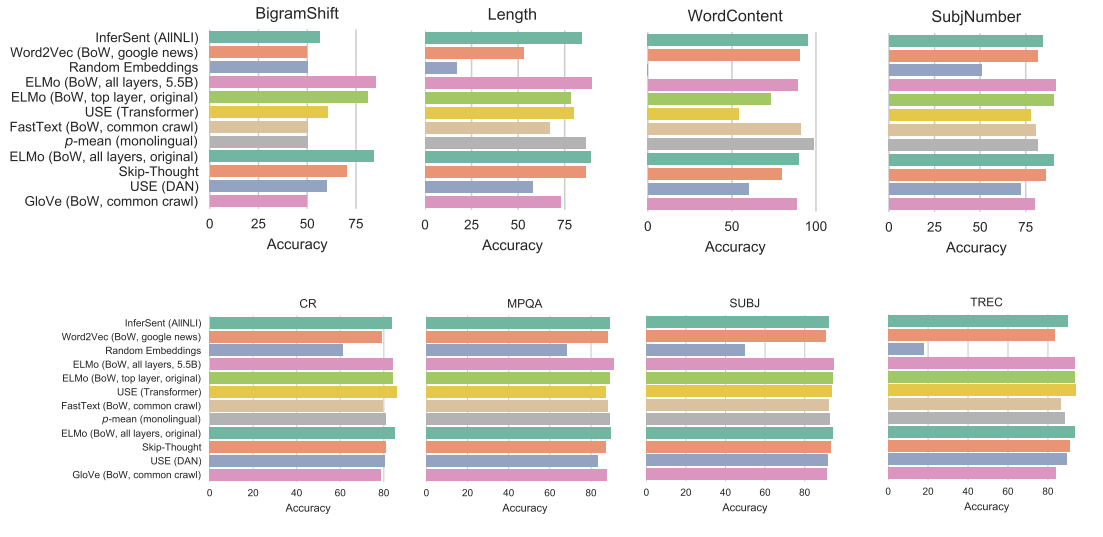
\includegraphics[scale=0.425]{images/results_perone}
	\caption[Results reported by Perone and colleagues]
		{Results for selected probing and downstream tasks as reported by \citep{Perone.2018}.}
	\label{fig:results_perone}
\end{figure}

Secondly, it is surprising that \textbf{random encoders score very highly in all languages}. The results we obtained show that such embeddings are able to outperform average embeddings (cf. \caps{TREC} task in English). \citep{Wieting.2019} find a similar pattern and therefore conclude that \textbf{random encoders \textit{`[constitute] a much stronger baseline'} than compositional models}. Comparing these results to \citep{Perone.2018} (cf. figure \vref{fig:results_perone}), one notices that they report the performance of random encoders to be substantially worse compared to the rest of the embeddings considered in their paper. Unfortunately, Perone and colleagues do not specify exactly how these embeddings were created. Differences can be caused by a different dimensionality or by a completely different encoding architecture. Despite the overall impressive performances of random encoders in this work, one can still identify a gap between those embeddings and trained sentence encoders in the English language. Nevertheless, these differences are much \textit{`smaller than [one] would have hoped'} to phrase it in the words of \citep{Wieting.2019}.

% Figure: Downstream task results
\begin{figure}
\begin{minipage}{0.265\textwidth}
\begin{tikzpicture}

  	\begin{axis}[
		title=ArgMin,
 	   	xbar stacked,
		bar width=4pt,
		enlarge y limits=0.2,
    		symbolic y coords={borep,rlstm,infers,laser,bert,qth,s2v,pms,avg},
		xmin=0,xmax=1,
  		xmajorgrids,
		tickwidth=0pt,
		xtick distance=0.40,
  		ytick=data,
		scale only axis=true,
  		width=3cm,height=2.5cm,
		tick label style={font=\tiny}
  	]

		% avg
  		\addplot[blue,fill] coordinates
  			{(0.550,avg) (0.00,pms) (0.00,s2v) (0.00,qth) (0.00,bert) (0.00,laser) (0.00,infers) (0.00,rlstm) (0.00,borep)};
		% pms
		\addplot[blue!50,fill] coordinates
			{(0.00,avg) (0.568,pms) (0.00,s2v) (0.00,qth) (0.00,bert) (0.00,laser) (0.00,infers) (0.00,rlstm) (0.00,borep)};

		% s2v
		\addplot[red,fill] coordinates 
			{(0.00,avg) (0.00,pms) (0.608,s2v) (0.00,qth) (0.00,bert) (0.00,laser) (0.00,infers) (0.00,rlstm) (0.00,borep)};
		% qth
		\addplot[red!60,fill] coordinates
			{(0.00,avg) (0.00,pms) (0.00,s2v) (0.581,qth) (0.00,bert) (0.00,laser) (0.00,infers) (0.00,rlstm) (0.00,borep)};
		% bert
		\addplot[red!40,fill] coordinates
			{(0.00,avg) (0.00,pms) (0.00,s2v) (0.00,qth) (0.558,bert) (0.00,laser) (0.00,infers) (0.00,rlstm) (0.00,borep)};
		% laser
		\addplot[red!20,fill] coordinates
			{(0.00,avg) (0.00,pms) (0.00,s2v) (0.00,qth) (0.00,bert) (0.596,laser) (0.00,infers) (0.00,rlstm) (0.00,borep)};
		% infers
		\addplot[red!10,fill] coordinates
			{(0.00,avg) (0.00,pms) (0.00,s2v) (0.00,qth) (0.00,bert) (0.00,laser) (0.604,infers) (0.00,rlstm) (0.00,borep)};

		% rand lstm
		\addplot[gray,fill] coordinates 
			{(0.00,avg) (0.00,pms) (0.00,s2v) (0.00,qth) (0.00,bert) (0.00,laser) (0.00,infers) (0.536,rlstm) (0.00,borep)};
		% borep
		\addplot[lightgray,fill] coordinates 
			{(0.00,avg) (0.00,pms) (0.00,s2v) (0.00,qth) (0.00,bert) (0.00,laser) (0.00,infers) (0.00,rlstm) (0.542,borep)};

  	\end{axis}



\end{tikzpicture}
\end{minipage}
\hfill
\begin{minipage}{0.25\textwidth}
\begin{tikzpicture}

  	\begin{axis}[
		title=Senti,
   	 	xbar stacked,
		bar width=4pt,
		enlarge y limits=0.2,
	    	symbolic y coords={borep,rlstm,infers,laser,bert,qth,s2v,pms,avg},
		xmin=0,xmax=1,
  		xmajorgrids,
		tickwidth=0pt,
		xtick distance=0.40,
  		ytick=data,
		yticklabels={,,},
		scale only axis=true,
  		width=3cm,height=2.5cm,
		tick label style={font=\tiny}
  	]

		% avg
  		\addplot[blue,fill] coordinates
  			{(0.698,avg) (0.00,pms) (0.00,s2v) (0.00,qth) (0.00,bert) (0.00,laser) (0.00,infers) (0.00,rlstm) (0.00,borep)};
		% pms
		\addplot[blue!50,fill] coordinates
			{(0.00,avg) (0.695,pms) (0.00,s2v) (0.00,qth) (0.00,bert) (0.00,laser) (0.00,infers) (0.00,rlstm) (0.00,borep)};

		% s2v
		\addplot[red,fill] coordinates 
			{(0.00,avg) (0.00,pms) (0.656,s2v) (0.00,qth) (0.00,bert) (0.00,laser) (0.00,infers) (0.00,rlstm) (0.00,borep)};
		% qth
		\addplot[red!60,fill] coordinates
			{(0.00,avg) (0.00,pms) (0.00,s2v) (0.636,qth) (0.00,bert) (0.00,laser) (0.00,infers) (0.00,rlstm) (0.00,borep)};
		% bert
		\addplot[red!40,fill] coordinates
			{(0.00,avg) (0.00,pms) (0.00,s2v) (0.00,qth) (0.644,bert) (0.00,laser) (0.00,infers) (0.00,rlstm) (0.00,borep)};
		% laser
		\addplot[red!20,fill] coordinates
			{(0.00,avg) (0.00,pms) (0.00,s2v) (0.00,qth) (0.00,bert) (0.727,laser) (0.00,infers) (0.00,rlstm) (0.00,borep)};
		% infers
		\addplot[red!10,fill] coordinates
			{(0.00,avg) (0.00,pms) (0.00,s2v) (0.00,qth) (0.00,bert) (0.00,laser) (0.702,infers) (0.00,rlstm) (0.00,borep)};

		% rand lstm
		\addplot[gray,fill] coordinates 
			{(0.00,avg) (0.00,pms) (0.00,s2v) (0.00,qth) (0.00,bert) (0.00,laser) (0.00,infers) (0.688,rlstm) (0.00,borep)};
		% borep
		\addplot[lightgray,fill] coordinates 
			{(0.00,avg) (0.00,pms) (0.00,s2v) (0.00,qth) (0.00,bert) (0.00,laser) (0.00,infers) (0.00,rlstm) (0.646,borep)};

  	\end{axis}

\end{tikzpicture}
\end{minipage}
\hfill
\begin{minipage}{0.25\textwidth}
\begin{tikzpicture}

  	\begin{axis}[
		title=TREC,
 	   	xbar stacked,
		bar width=4pt,
		enlarge y limits=0.2,
    		symbolic y coords={borep,rlstm,infers,laser,bert,qth,s2v,pms,avg},
		xmin=0,xmax=1,
  		xmajorgrids,
		tickwidth=0pt,
		xtick distance=0.40,
  		ytick=data,
		yticklabels={,,},
		scale only axis=true,
  		width=3cm,height=2.5cm,
		tick label style={font=\tiny}
  	]

		% avg
  		\addplot[blue,fill] coordinates
  			{(0.795,avg) (0.00,pms) (0.00,s2v) (0.00,qth) (0.00,bert) (0.00,laser) (0.00,infers) (0.00,rlstm) (0.00,borep)};
		% pms
		\addplot[blue!50,fill] coordinates
			{(0.00,avg) (0.767,pms) (0.00,s2v) (0.00,qth) (0.00,bert) (0.00,laser) (0.00,infers) (0.00,rlstm) (0.00,borep)};

		% s2v
		\addplot[red,fill] coordinates 
			{(0.00,avg) (0.00,pms) (0.792,s2v) (0.00,qth) (0.00,bert) (0.00,laser) (0.00,infers) (0.00,rlstm) (0.00,borep)};
		% qth
		\addplot[red!60,fill] coordinates
			{(0.00,avg) (0.00,pms) (0.00,s2v) (0.814,qth) (0.00,bert) (0.00,laser) (0.00,infers) (0.00,rlstm) (0.00,borep)};
		% bert
		\addplot[red!40,fill] coordinates
			{(0.00,avg) (0.00,pms) (0.00,s2v) (0.00,qth) (0.876,bert) (0.00,laser) (0.00,infers) (0.00,rlstm) (0.00,borep)};
		% laser
		\addplot[red!20,fill] coordinates
			{(0.00,avg) (0.00,pms) (0.00,s2v) (0.00,qth) (0.00,bert) (0.851,laser) (0.00,infers) (0.00,rlstm) (0.00,borep)};
		% infers
		\addplot[red!10,fill] coordinates
			{(0.00,avg) (0.00,pms) (0.00,s2v) (0.00,qth) (0.00,bert) (0.00,laser) (0.920,infers) (0.00,rlstm) (0.00,borep)};

		% rand lstm
		\addplot[gray,fill] coordinates 
			{(0.00,avg) (0.00,pms) (0.00,s2v) (0.00,qth) (0.00,bert) (0.00,laser) (0.00,infers) (0.774,rlstm) (0.00,borep)};
		% borep
		\addplot[lightgray,fill] coordinates 
			{(0.00,avg) (0.00,pms) (0.00,s2v) (0.00,qth) (0.00,bert) (0.00,laser) (0.00,infers) (0.00,rlstm) (0.819,borep)};

  	\end{axis}

\end{tikzpicture}
\end{minipage}
%\hfill
%\begin{minipage}{0.2\textwidth}
%\begin{tikzpicture}
%
%  	\begin{axis}[
%		title=SUBJ,
% 	   	xbar stacked,
%		bar width=4pt,
%		enlarge y limits=0.2,
%    		symbolic y coords={rlstm,infers,laser,bert,qth,s2v,pms,avg},
%		xmin=0,xmax=1,
%  		xmajorgrids,
%		tickwidth=0pt,
%		xtick distance=0.40,
%  		ytick=data,
%		yticklabels={,,},
%		scale only axis=true,
%  		width=3cm,height=2cm,
%		tick label style={font=\tiny}
%  	]
%
%		% avg
%  		\addplot[blue,fill] coordinates
%  			{(0.908,avg) (0.00,pms) (0.00,s2v) (0.00,qth) (0.00,bert) (0.00,laser) (0.00,infers) (0.00,rlstm)};
%		% pms
%		\addplot[blue!50,fill] coordinates
%			{(0.00,avg) (0.896,pms) (0.00,s2v) (0.00,qth) (0.00,bert) (0.00,laser) (0.00,infers) (0.00,rlstm)};
%
%		% s2v
%		\addplot[red,fill] coordinates 
%			{(0.00,avg) (0.00,pms) (0.920,s2v) (0.00,qth) (0.00,bert) (0.00,laser) (0.00,infers) (0.00,rlstm)};
%		% qth
%		\addplot[red!60,fill] coordinates
%			{(0.00,avg) (0.00,pms) (0.00,s2v) (0.816,qth) (0.00,bert) (0.00,laser) (0.00,infers) (0.00,rlstm)};
%		% bert
%		\addplot[red!40,fill] coordinates
%			{(0.00,avg) (0.00,pms) (0.00,s2v) (0.00,qth) (0.928,bert) (0.00,laser) (0.00,infers) (0.00,rlstm)};
%		% laser
%		\addplot[red!20,fill] coordinates
%			{(0.00,avg) (0.00,pms) (0.00,s2v) (0.00,qth) (0.00,bert) (0.914,laser) (0.00,infers) (0.00,rlstm)};
%		% infers
%		\addplot[red!20,fill] coordinates
%			{(0.00,avg) (0.00,pms) (0.00,s2v) (0.00,qth) (0.00,bert) (0.00,laser) (0.912,infers) (0.00,rlstm)};
%
%		% rand lstm
%		\addplot[gray,fill] coordinates 
%			{(0.00,avg) (0.00,pms) (0.00,s2v) (0.00,qth) (0.00,bert) (0.00,laser) (0.00,infers) (0.903,rlstm)};
%
%  	\end{axis}
%
%\end{tikzpicture}
%\end{minipage}
%\hfill
%\begin{minipage}{0.1\textwidth}
%\begin{tikzpicture}
%
%  	\begin{axis}[
%		title=Cluster,
%   	 	xbar stacked,
%		bar width=4pt,
%		enlarge y limits=0.2,
%	    	symbolic y coords={rlstm,infers,laser,bert,qth,s2v,pms,avg},
%		xmin=0,xmax=1,
%  		xmajorgrids,
%		tickwidth=0pt,
%		xtick distance=0.40,
%  		ytick=data,
%		yticklabels={,,},
%		scale only axis=true,
%  		width=1.3cm,height=2cm,
%		tick label style={font=\tiny}
%  	]
%
%		% avg
%  		\addplot[blue,fill] coordinates
%  			{(0.00,avg) (0.00,pms) (0.00,s2v) (0.00,qth) (0.00,bert) (0.00,laser) (0.00,infers) (0.00,rlstm)};
%		% pms
%		\addplot[blue!50,fill] coordinates
%			{(0.00,avg) (0.00,pms) (0.00,s2v) (0.00,qth) (0.00,bert) (0.00,laser) (0.00,infers) (0.00,rlstm)};
%
%		% s2v
%		\addplot[red,fill] coordinates 
%			{(0.00,avg) (0.00,pms) (0.00,s2v) (0.00,qth) (0.00,bert) (0.00,laser) (0.00,infers) (0.00,rlstm)};
%		% qth
%		\addplot[red!60,fill] coordinates
%			{(0.00,avg) (0.00,pms) (0.00,s2v) (0.00,qth) (0.00,bert) (0.00,laser) (0.00,infers) (0.00,rlstm)};
%		% bert
%		\addplot[red!40,fill] coordinates
%			{(0.00,avg) (0.00,pms) (0.00,s2v) (0.00,qth) (0.00,bert) (0.00,laser) (0.00,infers) (0.00,rlstm)};
%		% laser
%		\addplot[red!20,fill] coordinates
%			{(0.00,avg) (0.00,pms) (0.00,s2v) (0.00,qth) (0.00,bert) (0.00,laser) (0.00,infers) (0.00,rlstm)};
%		% infers
%		\addplot[red!20,fill] coordinates
%			{(0.00,avg) (0.00,pms) (0.00,s2v) (0.00,qth) (0.00,bert) (0.00,laser) (0.00,infers) (0.00,rlstm)};
%
%		% rand lstm
%		\addplot[gray,fill] coordinates 
%			{(0.00,avg) (0.00,pms) (0.00,s2v) (0.00,qth) (0.00,bert) (0.00,laser) (0.00,infers) (0.00,rlstm)};
%
%  	\end{axis}
%
%\end{tikzpicture}
%\end{minipage}
%\hfill
%\begin{minipage}{0.1\textwidth}
%\begin{tikzpicture}
%
%  	\begin{axis}[
%		title=MR,
%    		xbar stacked,
%		bar width=4pt,
%		enlarge y limits=0.2,
%    		symbolic y coords={rlstm,infers,laser,bert,qth,s2v,pms,avg},
%		xmin=0,xmax=1,
%  		xmajorgrids,
%		tickwidth=0pt,
%		xtick distance=0.40,
%  		ytick=data,
%		yticklabels={,,},
%		scale only axis=true,
%  		width=1.3cm,height=2cm,
%		tick label style={font=\tiny}
%  	]
%
%		% avg
%  		\addplot[blue,fill] coordinates
%  			{(0.763,avg) (0.00,pms) (0.00,s2v) (0.00,qth) (0.00,bert) (0.00,laser) (0.00,infers) (0.00,rlstm)};
%		% pms
%		\addplot[blue!50,fill] coordinates
%			{(0.00,avg) (0.753,pms) (0.00,s2v) (0.00,qth) (0.00,bert) (0.00,laser) (0.00,infers) (0.00,rlstm)};
%
%		% s2v
%		\addplot[red,fill] coordinates 
%			{(0.00,avg) (0.00,pms) (0.763,s2v) (0.00,qth) (0.00,bert) (0.00,laser) (0.00,infers) (0.00,rlstm)};
%		% qth
%		\addplot[red!60,fill] coordinates
%			{(0.00,avg) (0.00,pms) (0.00,s2v) (0.633,qth) (0.00,bert) (0.00,laser) (0.00,infers) (0.00,rlstm)};
%		% bert
%		\addplot[red!40,fill] coordinates
%			{(0.00,avg) (0.00,pms) (0.00,s2v) (0.00,qth) (0.683,bert) (0.00,laser) (0.00,infers) (0.00,rlstm)};
%		% laser
%		\addplot[red!20,fill] coordinates
%			{(0.00,avg) (0.00,pms) (0.00,s2v) (0.00,qth) (0.00,bert) (0.751,laser) (0.00,infers) (0.00,rlstm)};
%		% infers
%		\addplot[red!20,fill] coordinates
%			{(0.00,avg) (0.00,pms) (0.00,s2v) (0.00,qth) (0.00,bert) (0.00,laser) (0.748,infers) (0.00,rlstm)};
%
%		% rand lstm
%		\addplot[gray,fill] coordinates 
%			{(0.00,avg) (0.00,pms) (0.00,s2v) (0.00,qth) (0.00,bert) (0.00,laser) (0.00,infers) (0.745,rlstm)};
%
%  	\end{axis}
%
%\end{tikzpicture}
%\end{minipage}
%\hfill
%\begin{minipage}{0.1\textwidth}
%\begin{tikzpicture}
%
%  	\begin{axis}[
%		title=MPQA,
%  	  	xbar stacked,
%		bar width=4pt,
%		enlarge y limits=0.2,
%    		symbolic y coords={rlstm,infers,laser,bert,qth,s2v,pms,avg},
%		xmin=0,xmax=1,
%  		xmajorgrids,
%		tickwidth=0pt,
%		xtick distance=0.40,
%  		ytick=data,
%		yticklabels={,,},
%		scale only axis=true,
%  		width=1.3cm,height=2cm,
%		tick label style={font=\tiny}
%  	]
%
%		% avg
%  		\addplot[blue,fill] coordinates
%  			{(0.848,avg) (0.00,pms) (0.00,s2v) (0.00,qth) (0.00,bert) (0.00,laser) (0.00,infers) (0.00,rlstm)};
%		% pms
%		\addplot[blue!50,fill] coordinates
%			{(0.00,avg) (0.841,pms) (0.00,s2v) (0.00,qth) (0.00,bert) (0.00,laser) (0.00,infers) (0.00,rlstm)};
%
%		% s2v
%		\addplot[red,fill] coordinates 
%			{(0.00,avg) (0.00,pms) (0.848,s2v) (0.00,qth) (0.00,bert) (0.00,laser) (0.00,infers) (0.00,rlstm)};
%		% qth
%		\addplot[red!60,fill] coordinates
%			{(0.00,avg) (0.00,pms) (0.00,s2v) (0.724,qth) (0.00,bert) (0.00,laser) (0.00,infers) (0.00,rlstm)};
%		% bert
%		\addplot[red!40,fill] coordinates
%			{(0.00,avg) (0.00,pms) (0.00,s2v) (0.00,qth) (0.809,bert) (0.00,laser) (0.00,infers) (0.00,rlstm)};
%		% laser
%		\addplot[red!20,fill] coordinates
%			{(0.00,avg) (0.00,pms) (0.00,s2v) (0.00,qth) (0.00,bert) (0.855,laser) (0.00,infers) (0.00,rlstm)};
%		% infers
%		\addplot[red!20,fill] coordinates
%			{(0.00,avg) (0.00,pms) (0.00,s2v) (0.00,qth) (0.00,bert) (0.00,laser) (0.836,infers) (0.00,rlstm)};
%
%		% rand lstm
%		\addplot[gray,fill] coordinates 
%			{(0.00,avg) (0.00,pms) (0.00,s2v) (0.00,qth) (0.00,bert) (0.00,laser) (0.00,infers) (0.851,rlstm)};
%
%  	\end{axis}
%
%\end{tikzpicture}
%\end{minipage}
%\hfill
%\begin{minipage}{0.1\textwidth}
%\begin{tikzpicture}
%
%  	\begin{axis}[
%		title=CR,
% 	   	xbar stacked,
%		bar width=4pt,
%		enlarge y limits=0.2,
%    		symbolic y coords={rlstm,infers,laser,bert,qth,s2v,pms,avg},
%		xmin=0,xmax=1,
%  		xmajorgrids,
%		tickwidth=0pt,
%		xtick distance=0.40,
%  		ytick=data,
%		yticklabels={,,},
%		scale only axis=true,
%  		width=1.3cm,height=2cm,
%		tick label style={font=\tiny}
%  	]
%
%		% avg
%  		\addplot[blue,fill] coordinates
%  			{(0.772,avg) (0.00,pms) (0.00,s2v) (0.00,qth) (0.00,bert) (0.00,laser) (0.00,infers) (0.00,rlstm)};
%		% pms
%		\addplot[blue!50,fill] coordinates
%			{(0.00,avg) (0.743,pms) (0.00,s2v) (0.00,qth) (0.00,bert) (0.00,laser) (0.00,infers) (0.00,rlstm)};
%
%		% s2v
%		\addplot[red,fill] coordinates 
%			{(0.00,avg) (0.00,pms) (0.751,s2v) (0.00,qth) (0.00,bert) (0.00,laser) (0.00,infers) (0.00,rlstm)};
%		% qth
%		\addplot[red!60,fill] coordinates
%			{(0.00,avg) (0.00,pms) (0.00,s2v) (0.675,qth) (0.00,bert) (0.00,laser) (0.00,infers) (0.00,rlstm)};
%		% bert
%		\addplot[red!40,fill] coordinates
%			{(0.00,avg) (0.00,pms) (0.00,s2v) (0.00,qth) (0.744,bert) (0.00,laser) (0.00,infers) (0.00,rlstm)};
%		% laser
%		\addplot[red!20,fill] coordinates
%			{(0.00,avg) (0.00,pms) (0.00,s2v) (0.00,qth) (0.00,bert) (0.802,laser) (0.00,infers) (0.00,rlstm)};
%		% infers
%		\addplot[red!20,fill] coordinates
%			{(0.00,avg) (0.00,pms) (0.00,s2v) (0.00,qth) (0.00,bert) (0.00,laser) (0.711,infers) (0.00,rlstm)};
%
%		% rand lstm
%		\addplot[gray,fill] coordinates 
%			{(0.00,avg) (0.00,pms) (0.00,s2v) (0.00,qth) (0.00,bert) (0.00,laser) (0.00,infers) (0.761,rlstm)};
%
%  	\end{axis}
%
%\end{tikzpicture}
%\end{minipage}
\begin{center}
$\uparrow$ English
\end{center}
\begin{minipage}{0.265\textwidth}
\begin{tikzpicture}

  	\begin{axis}[
 	   	xbar stacked,
		bar width=4pt,
		enlarge y limits=0.2,
    		symbolic y coords={borep,rlstm,infers,laser,bert,qth,s2v,pms,avg},
		xmin=0,xmax=1,
  		xmajorgrids,
		tickwidth=0pt,
		xtick distance=0.40,
  		ytick=data,
		scale only axis=true,
  		width=3cm,height=2.5cm,
		tick label style={font=\tiny}
  	]

		% avg
  		\addplot[blue,fill] coordinates
  			{(0.507,avg) (0.00,pms) (0.00,s2v) (0.00,qth) (0.00,bert) (0.00,laser) (0.00,infers) (0.00,rlstm) (0.000,borep)};
		% pms
		\addplot[blue!50,fill] coordinates
			{(0.00,avg) (0.534,pms) (0.00,s2v) (0.00,qth) (0.00,bert) (0.00,laser) (0.00,infers) (0.00,rlstm) (0.000,borep)};

		% s2v
		\addplot[red,fill] coordinates 
			{(0.00,avg) (0.00,pms) (0.534,s2v) (0.00,qth) (0.00,bert) (0.00,laser) (0.00,infers) (0.00,rlstm) (0.000,borep)};
		% qth
		\addplot[red!60,fill] coordinates
			{(0.00,avg) (0.00,pms) (0.00,s2v) (0.497,qth) (0.00,bert) (0.00,laser) (0.00,infers) (0.00,rlstm) (0.000,borep)};
		% bert
		\addplot[red!40,fill] coordinates
			{(0.00,avg) (0.00,pms) (0.00,s2v) (0.00,qth) (0.517,bert) (0.00,laser) (0.00,infers) (0.00,rlstm) (0.000,borep)};
		% laser
		\addplot[red!20,fill] coordinates
			{(0.00,avg) (0.00,pms) (0.00,s2v) (0.00,qth) (0.00,bert) (0.583,laser) (0.00,infers) (0.00,rlstm) (0.000,borep)};
		% infersent
		\addplot[red!10,fill] coordinates
			{(0.00,avg) (0.00,pms) (0.00,s2v) (0.00,qth) (0.00,bert) (0.00,laser) (0.456,infers) (0.00,rlstm) (0.000,borep)};

		% rand lstm
		\addplot[gray,fill] coordinates 
			{(0.00,avg) (0.00,pms) (0.00,s2v) (0.00,qth) (0.00,bert) (0.00,laser) (0.00,infers) (0.507,rlstm) (0.000,borep)};
		% borep
		\addplot[lightgray,fill] coordinates 
			{(0.00,avg) (0.00,pms) (0.00,s2v) (0.00,qth) (0.00,bert) (0.00,laser) (0.00,infers) (0.00,rlstm) (0.507,borep)};

  	\end{axis}

\end{tikzpicture}
\end{minipage}
\hfill
\begin{minipage}{0.25\textwidth}
\begin{tikzpicture}

  	\begin{axis}[
   	 	xbar stacked,
		bar width=4pt,
		enlarge y limits=0.2,
	    	symbolic y coords={borep,rlstm,infers,laser,bert,qth,s2v,pms,avg},
		xmin=0,xmax=1,
  		xmajorgrids,
		tickwidth=0pt,
		xtick distance=0.40,
  		ytick=data,
		yticklabels={,,},
		scale only axis=true,
  		width=3cm,height=2.5cm,
		tick label style={font=\tiny}
  	]

		% avg
  		\addplot[blue,fill] coordinates
  			{(0.544,avg) (0.00,pms) (0.00,s2v) (0.00,qth) (0.00,bert) (0.00,laser) (0.00,infers) (0.00,rlstm) (0.000,borep)};
		% pms
		\addplot[blue!50,fill] coordinates
			{(0.00,avg) (0.550,pms) (0.00,s2v) (0.00,qth) (0.00,bert) (0.00,laser) (0.00,infers) (0.00,rlstm) (0.000,borep)};

		% s2v
		\addplot[red,fill] coordinates 
			{(0.00,avg) (0.00,pms) (0.590,s2v) (0.00,qth) (0.00,bert) (0.00,laser) (0.00,infers) (0.00,rlstm) (0.000,borep)};
		% qth
		\addplot[red!60,fill] coordinates
			{(0.00,avg) (0.00,pms) (0.00,s2v) (0.511,qth) (0.00,bert) (0.00,laser) (0.00,infers) (0.00,rlstm) (0.000,borep)};
		% bert
		\addplot[red!40,fill] coordinates
			{(0.00,avg) (0.00,pms) (0.00,s2v) (0.00,qth) (0.514,bert) (0.00,laser) (0.00,infers) (0.00,rlstm) (0.000,borep)};
		% laser
		\addplot[red!20,fill] coordinates
			{(0.00,avg) (0.00,pms) (0.00,s2v) (0.00,qth) (0.00,bert) (0.623,laser) (0.00,infers) (0.00,rlstm) (0.000,borep)};
		% infersent
		\addplot[red!10,fill] coordinates
			{(0.00,avg) (0.00,pms) (0.00,s2v) (0.00,qth) (0.00,bert) (0.00,laser) (0.547,infers) (0.00,rlstm) (0.000,borep)};

		% rand lstm
		\addplot[gray,fill] coordinates 
			{(0.00,avg) (0.00,pms) (0.00,s2v) (0.00,qth) (0.00,bert) (0.00,laser) (0.00,infers) (0.559,rlstm) (0.000,borep)};
		% borep
		\addplot[lightgray,fill] coordinates 
			{(0.00,avg) (0.00,pms) (0.00,s2v) (0.00,qth) (0.00,bert) (0.00,laser) (0.00,infers) (0.00,rlstm) (0.549,borep)};

  	\end{axis}

\end{tikzpicture}
\end{minipage}
\hfill
\begin{minipage}{0.25\textwidth}
\begin{tikzpicture}

  	\begin{axis}[
 	   	xbar stacked,
		bar width=4pt,
		enlarge y limits=0.2,
    		symbolic y coords={borep,rlstm,infers,laser,bert,qth,s2v,pms,avg},
		xmin=0,xmax=1,
  		xmajorgrids,
		tickwidth=0pt,
		xtick distance=0.40,
  		ytick=data,
		yticklabels={,,},
		scale only axis=true,
  		width=3cm,height=2.5cm,
		tick label style={font=\tiny}
  	]

		% avg
  		\addplot[blue,fill] coordinates
  			{(0.694,avg) (0.00,pms) (0.00,s2v) (0.00,qth) (0.00,bert) (0.00,laser) (0.00,infers) (0.00,rlstm) (0.000,borep)};
		% pms
		\addplot[blue!50,fill] coordinates
			{(0.00,avg) (0.765,pms) (0.00,s2v) (0.00,qth) (0.00,bert) (0.00,laser) (0.00,infers) (0.00,rlstm) (0.000,borep)};

		% s2v
		\addplot[red,fill] coordinates 
			{(0.00,avg) (0.00,pms) (0.846,s2v) (0.00,qth) (0.00,bert) (0.00,laser) (0.00,infers) (0.00,rlstm) (0.000,borep)};
		% qth
		\addplot[red!60,fill] coordinates
			{(0.00,avg) (0.00,pms) (0.00,s2v) (0.667,qth) (0.00,bert) (0.00,laser) (0.00,infers) (0.00,rlstm) (0.000,borep)};
		% bert
		\addplot[red!40,fill] coordinates
			{(0.00,avg) (0.00,pms) (0.00,s2v) (0.00,qth) (0.802,bert) (0.00,laser) (0.00,infers) (0.00,rlstm) (0.000,borep)};
		% laser
		\addplot[red!20,fill] coordinates
			{(0.00,avg) (0.00,pms) (0.00,s2v) (0.00,qth) (0.00,bert) (0.753,laser) (0.00,infers) (0.00,rlstm) (0.000,borep)};
		% infersent
		\addplot[red!10,fill] coordinates
			{(0.00,avg) (0.00,pms) (0.00,s2v) (0.00,qth) (0.00,bert) (0.00,laser) (0.580,infers) (0.00,rlstm) (0.000,borep)};

		% rand lstm
		\addplot[gray,fill] coordinates 
			{(0.00,avg) (0.00,pms) (0.00,s2v) (0.00,qth) (0.00,bert) (0.00,laser) (0.00,infers) (0.676,rlstm) (0.000,borep)};
		% borep
		\addplot[lightgray,fill] coordinates 
			{(0.00,avg) (0.00,pms) (0.00,s2v) (0.00,qth) (0.00,bert) (0.00,laser) (0.00,infers) (0.00,rlstm) (0.764,borep)};

  	\end{axis}

\end{tikzpicture}
\end{minipage}
%\hfill
%\begin{minipage}{0.1\textwidth}
%\begin{tikzpicture}
%
%  	\begin{axis}[
% 	   	xbar stacked,
%		bar width=4pt,
%		enlarge y limits=0.2,
%    		symbolic y coords={rlstm,infers,laser,bert,qth,s2v,pms,avg},
%		xmin=0,xmax=1,
%  		xmajorgrids,
%		tickwidth=0pt,
%		xtick distance=0.40,
%  		ytick=data,
%		yticklabels={,,},
%		scale only axis=true,
%  		width=1.3cm,height=2cm,
%		tick label style={font=\tiny}
%  	]
%
%		% avg
%  		\addplot[blue,fill] coordinates
%  			{(0.884,avg) (0.00,pms) (0.00,s2v) (0.00,qth) (0.00,bert) (0.00,laser) (0.00,infers) (0.00,rlstm)};
%		% pms
%		\addplot[blue!50,fill] coordinates
%			{(0.00,avg) (0.873,pms) (0.00,s2v) (0.00,qth) (0.00,bert) (0.00,laser) (0.00,infers) (0.00,rlstm)};
%
%		% s2v
%		\addplot[red,fill] coordinates 
%			{(0.00,avg) (0.00,pms) (0.867,s2v) (0.00,qth) (0.00,bert) (0.00,laser) (0.00,infers) (0.00,rlstm)};
%		% qth
%		\addplot[red!60,fill] coordinates
%			{(0.00,avg) (0.00,pms) (0.00,s2v) (0.831,qth) (0.00,bert) (0.00,laser) (0.00,infers) (0.00,rlstm)};
%		% bert
%		\addplot[red!40,fill] coordinates
%			{(0.00,avg) (0.00,pms) (0.00,s2v) (0.00,qth) (0.876,bert) (0.00,laser) (0.00,infers) (0.00,rlstm)};
%		% laser
%		\addplot[red!20,fill] coordinates
%			{(0.00,avg) (0.00,pms) (0.00,s2v) (0.00,qth) (0.00,bert) (0.906,laser) (0.00,infers) (0.00,rlstm)};
%		% infersent
%		\addplot[red!10,fill] coordinates
%			{(0.00,avg) (0.00,pms) (0.00,s2v) (0.00,qth) (0.00,bert) (0.00,laser) (0.875,infers) (0.00,rlstm)};
%
%		% rand lstm
%		\addplot[gray,fill] coordinates 
%			{(0.00,avg) (0.00,pms) (0.00,s2v) (0.00,qth) (0.00,bert) (0.00,laser) (0.00,infers) (0.874,rlstm)};
%
%  	\end{axis}
%
%\end{tikzpicture}
%\end{minipage}
%\hfill
%\begin{minipage}{0.1\textwidth}
%\begin{tikzpicture}
%
%  	\begin{axis}[
%   	 	xbar stacked,
%		bar width=4pt,
%		enlarge y limits=0.2,
%	    	symbolic y coords={rlstm,infers,laser,bert,qth,s2v,pms,avg},
%		xmin=0,xmax=1,
%  		xmajorgrids,
%		tickwidth=0pt,
%		xtick distance=0.40,
%  		ytick=data,
%		yticklabels={,,},
%		scale only axis=true,
%  		width=1.3cm,height=2cm,
%		tick label style={font=\tiny}
%  	]
%
%		% avg
%  		\addplot[blue,fill] coordinates
%  			{(0.00,avg) (0.00,pms) (0.00,s2v) (0.00,qth) (0.00,bert) (0.00,laser) (0.00,infers) (0.00,rlstm)};
%		% pms
%		\addplot[blue!50,fill] coordinates
%			{(0.00,avg) (0.00,pms) (0.00,s2v) (0.00,qth) (0.00,bert) (0.00,laser) (0.00,infers) (0.00,rlstm)};
%
%		% s2v
%		\addplot[red,fill] coordinates 
%			{(0.00,avg) (0.00,pms) (0.00,s2v) (0.00,qth) (0.00,bert) (0.00,laser) (0.00,infers) (0.00,rlstm)};
%		% qth
%		\addplot[red!60,fill] coordinates
%			{(0.00,avg) (0.00,pms) (0.00,s2v) (0.00,qth) (0.00,bert) (0.00,laser) (0.00,infers) (0.00,rlstm)};
%		% bert
%		\addplot[red!40,fill] coordinates
%			{(0.00,avg) (0.00,pms) (0.00,s2v) (0.00,qth) (0.00,bert) (0.00,laser) (0.00,infers) (0.00,rlstm)};
%		% laser
%		\addplot[red!20,fill] coordinates
%			{(0.00,avg) (0.00,pms) (0.00,s2v) (0.00,qth) (0.00,bert) (0.00,laser) (0.00,infers) (0.00,rlstm)};
%
%		% rand lstm
%		\addplot[gray,fill] coordinates 
%			{(0.00,avg) (0.00,pms) (0.00,s2v) (0.00,qth) (0.00,bert) (0.00,laser) (0.00,infers) (0.00,rlstm)};
%
%  	\end{axis}
%
%\end{tikzpicture}
%\end{minipage}
%\hfill
%\begin{minipage}{0.1\textwidth}
%\begin{center}
%\textit{n.\,a.}
%\end{center}
%\end{minipage}
%\hfill
%\begin{minipage}{0.1\textwidth}
%\begin{center}
%\textit{n.\,a.}
%\end{center}
%\end{minipage}
%\hfill
%\begin{minipage}{0.1\textwidth}
%\begin{center}
%\textit{n.\,a.}
%\end{center}
%\end{minipage}
\begin{center}
$\uparrow$ German
\end{center}
\begin{minipage}{0.265\textwidth}
\begin{tikzpicture}

  	\begin{axis}[
 	   	xbar stacked,
		bar width=4pt,
		enlarge y limits=0.2,
    		symbolic y coords={borep,rlstm,infers,laser,bert,qth,s2v,pms,avg},
		xmin=0,xmax=1,
  		xmajorgrids,
		tickwidth=0pt,
		xtick distance=0.40,
  		ytick=data,
		scale only axis=true,
  		width=3cm,height=2.5cm,
		tick label style={font=\tiny}
  	]

		% avg
  		\addplot[blue,fill] coordinates
  			{(0.535,avg) (0.00,pms) (0.00,s2v) (0.00,qth) (0.00,bert) (0.00,laser) (0.00,infers) (0.00,rlstm) (0.000,borep)};
		% pms
		\addplot[blue!50,fill] coordinates
			{(0.00,avg) (0.553,pms) (0.00,s2v) (0.00,qth) (0.00,bert) (0.00,laser) (0.00,infers) (0.00,rlstm) (0.000,borep)};

		% s2v
		\addplot[red,fill] coordinates 
			{(0.00,avg) (0.00,pms) (0.534,s2v) (0.00,qth) (0.00,bert) (0.00,laser) (0.00,infers) (0.00,rlstm) (0.000,borep)};
		% qth
		\addplot[red!60,fill] coordinates
			{(0.00,avg) (0.00,pms) (0.00,s2v) (0.540,qth) (0.00,bert) (0.00,laser) (0.00,infers) (0.00,rlstm) (0.000,borep)};
		% bert
		\addplot[red!40,fill] coordinates
			{(0.00,avg) (0.00,pms) (0.00,s2v) (0.00,qth) (0.531,bert) (0.00,laser) (0.00,infers) (0.00,rlstm) (0.000,borep)};
		% laser
		\addplot[red!20,fill] coordinates
			{(0.00,avg) (0.00,pms) (0.00,s2v) (0.00,qth) (0.00,bert) (0.582,laser) (0.00,infers) (0.00,rlstm) (0.000,borep)};
		% infersent
		\addplot[red!10,fill] coordinates
			{(0.00,avg) (0.00,pms) (0.00,s2v) (0.00,qth) (0.00,bert) (0.00,laser) (0.487,infers) (0.00,rlstm) (0.000,borep)};

		% rand lstm
		\addplot[gray,fill] coordinates 
			{(0.00,avg) (0.00,pms) (0.00,s2v) (0.00,qth) (0.00,bert) (0.00,laser) (0.00,infers) (0.521,rlstm) (0.000,borep)};
		% borep
		\addplot[lightgray,fill] coordinates 
			{(0.00,avg) (0.00,pms) (0.00,s2v) (0.00,qth) (0.00,bert) (0.00,laser) (0.00,infers) (0.00,rlstm) (0.518,borep)};

  	\end{axis}

\end{tikzpicture}
\end{minipage}
\hfill
\begin{minipage}{0.25\textwidth}
\begin{tikzpicture}

  	\begin{axis}[
   	 	xbar stacked,
		bar width=4pt,
		enlarge y limits=0.2,
	    	symbolic y coords={borep,rlstm,infers,laser,bert,qth,s2v,pms,avg},
		xmin=0,xmax=1,
  		xmajorgrids,
		tickwidth=0pt,
		xtick distance=0.40,
  		ytick=data,
		yticklabels={,,},
		scale only axis=true,
  		width=3cm,height=2.5cm,
		tick label style={font=\tiny}
  	]

		% avg
  		\addplot[blue,fill] coordinates
  			{(0.703,avg) (0.00,pms) (0.00,s2v) (0.00,qth) (0.00,bert) (0.00,laser) (0.00,infers) (0.00,rlstm) (0.000,borep)};
		% pms
		\addplot[blue!50,fill] coordinates
			{(0.00,avg) (0.695,pms) (0.00,s2v) (0.00,qth) (0.00,bert) (0.00,laser) (0.00,infers) (0.00,rlstm) (0.000,borep)};

		% s2v
		\addplot[red,fill] coordinates 
			{(0.00,avg) (0.00,pms) (0.622,s2v) (0.00,qth) (0.00,bert) (0.00,laser) (0.00,infers) (0.00,rlstm) (0.000,borep)};
		% qth
		\addplot[red!60,fill] coordinates
			{(0.00,avg) (0.00,pms) (0.00,s2v) (0.627,qth) (0.00,bert) (0.00,laser) (0.00,infers) (0.00,rlstm) (0.000,borep)};
		% bert
		\addplot[red!40,fill] coordinates
			{(0.00,avg) (0.00,pms) (0.00,s2v) (0.00,qth) (0.644,bert) (0.00,laser) (0.00,infers) (0.00,rlstm) (0.000,borep)};
		% laser
		\addplot[red!20,fill] coordinates
			{(0.00,avg) (0.00,pms) (0.00,s2v) (0.00,qth) (0.00,bert) (0.728,laser) (0.00,infers) (0.00,rlstm) (0.000,borep)};
		% infersent
		\addplot[red!10,fill] coordinates
			{(0.00,avg) (0.00,pms) (0.00,s2v) (0.00,qth) (0.00,bert) (0.00,laser) (0.676,infers) (0.00,rlstm) (0.000,borep)};

		% rand lstm
		\addplot[gray,fill] coordinates 
			{(0.00,avg) (0.00,pms) (0.00,s2v) (0.00,qth) (0.00,bert) (0.00,laser) (0.00,infers) (0.695,rlstm) (0.000,borep)};
		% borep
		\addplot[lightgray,fill] coordinates 
			{(0.00,avg) (0.00,pms) (0.00,s2v) (0.00,qth) (0.00,bert) (0.00,laser) (0.00,infers) (0.00,rlstm) (0.643,borep)};

  	\end{axis}

\end{tikzpicture}
\end{minipage}
\hfill
\begin{minipage}{0.25\textwidth}
\begin{tikzpicture}

  	\begin{axis}[
 	   	xbar stacked,
		bar width=4pt,
		enlarge y limits=0.2,
    		symbolic y coords={borep,rlstm,infers,laser,bert,qth,s2v,pms,avg},
		xmin=0,xmax=1,
  		xmajorgrids,
		tickwidth=0pt,
		xtick distance=0.40,
  		ytick=data,
		yticklabels={,,},
		scale only axis=true,
  		width=3cm,height=2.5cm,
		tick label style={font=\tiny}
  	]

		% avg
  		\addplot[blue,fill] coordinates
  			{(0.767,avg) (0.00,pms) (0.00,s2v) (0.00,qth) (0.00,bert) (0.00,laser) (0.00,infers) (0.00,rlstm) (0.000,borep)};
		% pms
		\addplot[blue!50,fill] coordinates
			{(0.00,avg) (0.799,pms) (0.00,s2v) (0.00,qth) (0.00,bert) (0.00,laser) (0.00,infers) (0.00,rlstm) (0.000,borep)};

		% s2v
		\addplot[red,fill] coordinates 
			{(0.00,avg) (0.00,pms) (0.832,s2v) (0.00,qth) (0.00,bert) (0.00,laser) (0.00,infers) (0.00,rlstm) (0.000,borep)};
		% qth
		\addplot[red!60,fill] coordinates
			{(0.00,avg) (0.00,pms) (0.00,s2v) (0.780,qth) (0.00,bert) (0.00,laser) (0.00,infers) (0.00,rlstm) (0.000,borep)};
		% bert
		\addplot[red!40,fill] coordinates
			{(0.00,avg) (0.00,pms) (0.00,s2v) (0.00,qth) (0.822,bert) (0.00,laser) (0.00,infers) (0.00,rlstm) (0.000,borep)};
		% laser
		\addplot[red!20,fill] coordinates
			{(0.00,avg) (0.00,pms) (0.00,s2v) (0.00,qth) (0.00,bert) (0.728,laser) (0.00,infers) (0.00,rlstm) (0.000,borep)};
		% infersent
		\addplot[red!10,fill] coordinates
			{(0.00,avg) (0.00,pms) (0.00,s2v) (0.00,qth) (0.00,bert) (0.00,laser) (0.623,infers) (0.00,rlstm) (0.000,borep)};

		% rand lstm
		\addplot[gray,fill] coordinates 
			{(0.00,avg) (0.00,pms) (0.00,s2v) (0.00,qth) (0.00,bert) (0.00,laser) (0.00,infers) (0.739,rlstm) (0.000,borep)};
		% borep
		\addplot[lightgray,fill] coordinates 
			{(0.00,avg) (0.00,pms) (0.00,s2v) (0.00,qth) (0.00,bert) (0.00,laser) (0.00,infers) (0.00,rlstm) (0.778,borep)};

  	\end{axis}

\end{tikzpicture}
\end{minipage}
%\hfill
%\begin{minipage}{0.1\textwidth}
%\begin{tikzpicture}
%
%  	\begin{axis}[
% 	   	xbar stacked,
%		bar width=4pt,
%		enlarge y limits=0.2,
%    		symbolic y coords={rlstm,infers,laser,bert,qth,s2v,pms,avg},
%		xmin=0,xmax=1,
%  		xmajorgrids,
%		tickwidth=0pt,
%		xtick distance=0.40,
%  		ytick=data,
%		yticklabels={,,},
%		scale only axis=true,
%  		width=1.3cm,height=2cm,
%		tick label style={font=\tiny}
%  	]
%
%		% avg
%  		\addplot[blue,fill] coordinates
%  			{(0.884,avg) (0.00,pms) (0.00,s2v) (0.00,qth) (0.00,bert) (0.00,laser) (0.00,infers) (0.00,rlstm)};
%		% pms
%		\addplot[blue!50,fill] coordinates
%			{(0.00,avg) (0.871,pms) (0.00,s2v) (0.00,qth) (0.00,bert) (0.00,laser) (0.00,infers) (0.00,rlstm)};
%
%		% s2v
%		\addplot[red,fill] coordinates 
%			{(0.00,avg) (0.00,pms) (0.870,s2v) (0.00,qth) (0.00,bert) (0.00,laser) (0.00,infers) (0.00,rlstm)};
%		% qth
%		\addplot[red!60,fill] coordinates
%			{(0.00,avg) (0.00,pms) (0.00,s2v) (0.863,qth) (0.00,bert) (0.00,laser) (0.00,infers) (0.00,rlstm)};
%		% bert
%		\addplot[red!40,fill] coordinates
%			{(0.00,avg) (0.00,pms) (0.00,s2v) (0.00,qth) (0.885,bert) (0.00,laser) (0.00,infers) (0.00,rlstm)};
%		% laser
%		\addplot[red!20,fill] coordinates
%			{(0.00,avg) (0.00,pms) (0.00,s2v) (0.00,qth) (0.00,bert) (0.901,laser) (0.00,infers) (0.00,rlstm)};
%		% infersent
%		\addplot[red!20,fill] coordinates
%			{(0.00,avg) (0.00,pms) (0.00,s2v) (0.00,qth) (0.00,bert) (0.00,laser) (0.870,infers) (0.00,rlstm)};
%
%		% rand lstm
%		\addplot[gray,fill] coordinates 
%			{(0.00,avg) (0.00,pms) (0.00,s2v) (0.00,qth) (0.00,bert) (0.00,laser) (0.00,infers) (0.871,rlstm)};
%
%  	\end{axis}
%
%\end{tikzpicture}
%\end{minipage}
%\hfill
%\begin{minipage}{0.1\textwidth}
%\begin{tikzpicture}
%
%  	\begin{axis}[
%   	 	xbar stacked,
%		bar width=4pt,
%		enlarge y limits=0.2,
%	    	symbolic y coords={rlstm,infers,laser,bert,qth,s2v,pms,avg},
%		xmin=0,xmax=1,
%  		xmajorgrids,
%		tickwidth=0pt,
%		xtick distance=0.40,
%  		ytick=data,
%		yticklabels={,,},
%		scale only axis=true,
%  		width=1.3cm,height=2cm,
%		tick label style={font=\tiny}
%  	]
%
%		% avg
%  		\addplot[blue,fill] coordinates
%  			{(0.00,avg) (0.00,pms) (0.00,s2v) (0.00,qth) (0.00,bert) (0.00,laser) (0.00,infers) (0.00,rlstm)};
%		% pms
%		\addplot[blue!50,fill] coordinates
%			{(0.00,avg) (0.00,pms) (0.00,s2v) (0.00,qth) (0.00,bert) (0.00,laser) (0.00,infers) (0.00,rlstm)};
%
%		% s2v
%		\addplot[red,fill] coordinates 
%			{(0.00,avg) (0.00,pms) (0.00,s2v) (0.00,qth) (0.00,bert) (0.00,laser) (0.00,infers) (0.00,rlstm)};
%		% qth
%		\addplot[red!60,fill] coordinates
%			{(0.00,avg) (0.00,pms) (0.00,s2v) (0.00,qth) (0.00,bert) (0.00,laser) (0.00,infers) (0.00,rlstm)};
%		% bert
%		\addplot[red!40,fill] coordinates
%			{(0.00,avg) (0.00,pms) (0.00,s2v) (0.00,qth) (0.00,bert) (0.00,laser) (0.00,infers) (0.00,rlstm)};
%		% laser
%		\addplot[red!20,fill] coordinates
%			{(0.00,avg) (0.00,pms) (0.00,s2v) (0.00,qth) (0.00,bert) (0.00,laser) (0.00,infers) (0.00,rlstm)};
%		% infersent
%		\addplot[red!20,fill] coordinates
%			{(0.00,avg) (0.00,pms) (0.00,s2v) (0.00,qth) (0.00,bert) (0.00,laser) (0.00,infers) (0.00,rlstm)};
%
%		% rand lstm
%		\addplot[gray,fill] coordinates 
%			{(0.00,avg) (0.00,pms) (0.00,s2v) (0.00,qth) (0.00,bert) (0.00,laser) (0.00,infers) (0.00,rlstm)};
%
%  	\end{axis}
%
%\end{tikzpicture}
%\end{minipage}
%\hfill
%\begin{minipage}{0.1\textwidth}
%\begin{center}
%\textit{n.\,a.}
%\end{center}
%\end{minipage}
%\hfill
%\begin{minipage}{0.1\textwidth}
%\begin{center}
%\textit{n.\,a.}
%\end{center}
%\end{minipage}
%\hfill
%\begin{minipage}{0.1\textwidth}
%\begin{center}
%\textit{n.\,a.}
%\end{center}
%\end{minipage}
\begin{center}
$\uparrow$ Russian
\end{center}
\begin{minipage}{0.265\textwidth}
\begin{tikzpicture}

  	\begin{axis}[
 	   	xbar stacked,
		bar width=4pt,
		enlarge y limits=0.2,
    		symbolic y coords={borep,rlstm,infers,laser,bert,qth,s2v,pms,avg},
		xmin=0,xmax=1,
  		xmajorgrids,
		tickwidth=0pt,
		xtick distance=0.40,
  		ytick=data,
		scale only axis=true,
  		width=3cm,height=2.5cm,
		tick label style={font=\tiny}
  	]

		% avg
  		\addplot[blue,fill] coordinates
  			{(0.525,avg) (0.00,pms) (0.00,s2v) (0.00,qth) (0.00,bert) (0.00,laser) (0.00,infers) (0.00,rlstm) (0.000,borep)};
		% pms
		\addplot[blue!50,fill] coordinates
			{(0.00,avg) (0.547,pms) (0.00,s2v) (0.00,qth) (0.00,bert) (0.00,laser) (0.00,infers) (0.00,rlstm) (0.000,borep)};

		% s2v
		\addplot[red,fill] coordinates 
			{(0.00,avg) (0.00,pms) (0.504,s2v) (0.00,qth) (0.00,bert) (0.00,laser) (0.00,infers) (0.00,rlstm) (0.000,borep)};
		% qth
		\addplot[red!60,fill] coordinates
			{(0.00,avg) (0.00,pms) (0.00,s2v) (0.515,qth) (0.00,bert) (0.00,laser) (0.00,infers) (0.00,rlstm) (0.000,borep)};
		% bert
		\addplot[red!40,fill] coordinates
			{(0.00,avg) (0.00,pms) (0.00,s2v) (0.00,qth) (0.493,bert) (0.00,laser) (0.00,infers) (0.00,rlstm) (0.000,borep)};
		% laser
		\addplot[red!20,fill] coordinates
			{(0.00,avg) (0.00,pms) (0.00,s2v) (0.00,qth) (0.00,bert) (0.555,laser) (0.00,infers) (0.00,rlstm) (0.000,borep)};
		% infersent
		\addplot[red!10,fill] coordinates
			{(0.00,avg) (0.00,pms) (0.00,s2v) (0.00,qth) (0.00,bert) (0.00,laser) (0.510,infers) (0.00,rlstm) (0.000,borep)};

		% rand lstm
		\addplot[gray,fill] coordinates 
			{(0.00,avg) (0.00,pms) (0.00,s2v) (0.00,qth) (0.00,bert) (0.00,laser) (0.00,infers) (0.515,rlstm) (0.000,borep)};
		% borep
		\addplot[lightgray,fill] coordinates 
			{(0.00,avg) (0.00,pms) (0.00,s2v) (0.00,qth) (0.00,bert) (0.00,laser) (0.00,infers) (0.00,rlstm) (0.512,borep)};

  	\end{axis}

\end{tikzpicture}
\end{minipage}
\hfill
\begin{minipage}{0.25\textwidth}
\begin{tikzpicture}

  	\begin{axis}[
   	 	xbar stacked,
		bar width=4pt,
		enlarge y limits=0.2,
	    	symbolic y coords={borep,rlstm,infers,laser,bert,qth,s2v,pms,avg},
		xmin=0,xmax=1,
  		xmajorgrids,
		tickwidth=0pt,
		xtick distance=0.40,
  		ytick=data,
		yticklabels={,,},
		scale only axis=true,
  		width=3cm,height=2.5cm,
		tick label style={font=\tiny}
  	]

		% avg
  		\addplot[blue,fill] coordinates
  			{(0.529,avg) (0.00,pms) (0.00,s2v) (0.00,qth) (0.00,bert) (0.00,laser) (0.00,infers) (0.00,rlstm) (0.000,borep)};
		% pms
		\addplot[blue!50,fill] coordinates
			{(0.00,avg) (0.511,pms) (0.00,s2v) (0.00,qth) (0.00,bert) (0.00,laser) (0.00,infers) (0.00,rlstm) (0.000,borep)};

		% s2v
		\addplot[red,fill] coordinates 
			{(0.00,avg) (0.00,pms) (0.483,s2v) (0.00,qth) (0.00,bert) (0.00,laser) (0.00,infers) (0.00,rlstm) (0.000,borep)};
		% qth
		\addplot[red!60,fill] coordinates
			{(0.00,avg) (0.00,pms) (0.00,s2v) (0.469,qth) (0.00,bert) (0.00,laser) (0.00,infers) (0.00,rlstm) (0.000,borep)};
		% bert
		\addplot[red!40,fill] coordinates
			{(0.00,avg) (0.00,pms) (0.00,s2v) (0.00,qth) (0.484,bert) (0.00,laser) (0.00,infers) (0.00,rlstm) (0.000,borep)};
		% laser
		\addplot[red!20,fill] coordinates
			{(0.00,avg) (0.00,pms) (0.00,s2v) (0.00,qth) (0.00,bert) (0.523,laser) (0.00,infers) (0.00,rlstm) (0.000,borep)};
		% infersent
		\addplot[red!10,fill] coordinates
			{(0.00,avg) (0.00,pms) (0.00,s2v) (0.00,qth) (0.00,bert) (0.00,laser) (0.514,infers) (0.00,rlstm) (0.000,borep)};

		% rand lstm
		\addplot[gray,fill] coordinates 
			{(0.00,avg) (0.00,pms) (0.00,s2v) (0.00,qth) (0.00,bert) (0.00,laser) (0.00,infers) (0.529,rlstm) (0.000,borep)};
		% borep
		\addplot[lightgray,fill] coordinates 
			{(0.00,avg) (0.00,pms) (0.00,s2v) (0.00,qth) (0.00,bert) (0.00,laser) (0.00,infers) (0.00,rlstm) (0.498,borep)};

  	\end{axis}

\end{tikzpicture}
\end{minipage}
\hfill
\begin{minipage}{0.25\textwidth}
\begin{tikzpicture}

  	\begin{axis}[
 	   	xbar stacked,
		bar width=4pt,
		enlarge y limits=0.2,
    		symbolic y coords={borep,rlstm,infers,laser,bert,qth,s2v,pms,avg},
		xmin=0,xmax=1,
  		xmajorgrids,
		tickwidth=0pt,
		xtick distance=0.40,
  		ytick=data,
		yticklabels={,,},
		scale only axis=true,
  		width=3cm,height=2.5cm,
		tick label style={font=\tiny}
  	]

		% avg
  		\addplot[blue,fill] coordinates
  			{(0.649,avg) (0.00,pms) (0.00,s2v) (0.00,qth) (0.00,bert) (0.00,laser) (0.00,infers) (0.00,rlstm) (0.000,borep)};
		% pms
		\addplot[blue!50,fill] coordinates
			{(0.00,avg) (0.683,pms) (0.00,s2v) (0.00,qth) (0.00,bert) (0.00,laser) (0.00,infers) (0.00,rlstm) (0.000,borep)};

		% s2v
		\addplot[red,fill] coordinates 
			{(0.00,avg) (0.00,pms) (0.698,s2v) (0.00,qth) (0.00,bert) (0.00,laser) (0.00,infers) (0.00,rlstm) (0.000,borep)};
		% qth
		\addplot[red!60,fill] coordinates
			{(0.00,avg) (0.00,pms) (0.00,s2v) (0.650,qth) (0.00,bert) (0.00,laser) (0.00,infers) (0.00,rlstm) (0.000,borep)};
		% bert
		\addplot[red!40,fill] coordinates
			{(0.00,avg) (0.00,pms) (0.00,s2v) (0.00,qth) (0.695,bert) (0.00,laser) (0.00,infers) (0.00,rlstm) (0.000,borep)};
		% laser
		\addplot[red!20,fill] coordinates
			{(0.00,avg) (0.00,pms) (0.00,s2v) (0.00,qth) (0.00,bert) (0.660,laser) (0.00,infers) (0.00,rlstm) (0.000,borep)};
		% infersent
		\addplot[red!10,fill] coordinates
			{(0.00,avg) (0.00,pms) (0.00,s2v) (0.00,qth) (0.00,bert) (0.00,laser) (0.545,infers) (0.00,rlstm) (0.000,borep)};

		% rand lstm
		\addplot[gray,fill] coordinates 
			{(0.00,avg) (0.00,pms) (0.00,s2v) (0.00,qth) (0.00,bert) (0.00,laser) (0.00,infers) (0.685,rlstm) (0.000,borep)};
		% borep
		\addplot[lightgray,fill] coordinates 
			{(0.00,avg) (0.00,pms) (0.00,s2v) (0.00,qth) (0.00,bert) (0.00,laser) (0.00,infers) (0.00,rlstm) (0.722,borep)};

  	\end{axis}

\end{tikzpicture}
\end{minipage}
%\hfill
%\begin{minipage}{0.1\textwidth}
%\begin{tikzpicture}
%
%  	\begin{axis}[
% 	   	xbar stacked,
%		bar width=4pt,
%		enlarge y limits=0.2,
%    		symbolic y coords={rlstm,infers,laser,bert,qth,s2v,pms,avg},
%		xmin=0,xmax=1,
%  		xmajorgrids,
%		tickwidth=0pt,
%		xtick distance=0.40,
%  		ytick=data,
%		yticklabels={,,},
%		scale only axis=true,
%  		width=1.3cm,height=2cm,
%		tick label style={font=\tiny}
%  	]
%
%		% avg
%  		\addplot[blue,fill] coordinates
%  			{(0.862,avg) (0.00,pms) (0.00,s2v) (0.00,qth) (0.00,bert) (0.00,laser) (0.00,infers) (0.00,rlstm)};
%		% pms
%		\addplot[blue!50,fill] coordinates
%			{(0.00,avg) (0.851,pms) (0.00,s2v) (0.00,qth) (0.00,bert) (0.00,laser) (0.00,infers) (0.00,rlstm)};
%
%		% s2v
%		\addplot[red,fill] coordinates 
%			{(0.00,avg) (0.00,pms) (0.832,s2v) (0.00,qth) (0.00,bert) (0.00,laser) (0.00,infers) (0.00,rlstm)};
%		% qth
%		\addplot[red!60,fill] coordinates
%			{(0.00,avg) (0.00,pms) (0.00,s2v) (0.431,qth) (0.00,bert) (0.00,laser) (0.00,infers) (0.00,rlstm)};
%		% bert
%		\addplot[red!40,fill] coordinates
%			{(0.00,avg) (0.00,pms) (0.00,s2v) (0.00,qth) (0.819,bert) (0.00,laser) (0.00,infers) (0.00,rlstm)};
%		% laser
%		\addplot[red!20,fill] coordinates
%			{(0.00,avg) (0.00,pms) (0.00,s2v) (0.00,qth) (0.00,bert) (0.886,laser) (0.00,infers) (0.00,rlstm)};
%		% infersent
%		\addplot[red!20,fill] coordinates
%			{(0.00,avg) (0.00,pms) (0.00,s2v) (0.00,qth) (0.00,bert) (0.00,laser) (0.850,infers) (0.00,rlstm)};
%
%		% rand lstm
%		\addplot[gray,fill] coordinates 
%			{(0.00,avg) (0.00,pms) (0.00,s2v) (0.00,qth) (0.00,bert) (0.00,laser) (0.00,infers) (0.854,rlstm)};
%
%  	\end{axis}
%
%\end{tikzpicture}
%\end{minipage}
%\hfill
%\begin{minipage}{0.1\textwidth}
%\begin{tikzpicture}
%
%  	\begin{axis}[
%   	 	xbar stacked,
%		bar width=4pt,
%		enlarge y limits=0.2,
%	    	symbolic y coords={rlstm,infers,laser,bert,qth,s2v,pms,avg},
%		xmin=0,xmax=1,
%  		xmajorgrids,
%		tickwidth=0pt,
%		xtick distance=0.40,
%  		ytick=data,
%		yticklabels={,,},
%		scale only axis=true,
%  		width=1.3cm,height=2cm,
%		tick label style={font=\tiny}
%  	]
%
%		% avg
%  		\addplot[blue,fill] coordinates
%  			{(0.00,avg) (0.00,pms) (0.00,s2v) (0.00,qth) (0.00,bert) (0.00,laser) (0.00,infers) (0.00,rlstm)};
%		% pms
%		\addplot[blue!50,fill] coordinates
%			{(0.00,avg) (0.00,pms) (0.00,s2v) (0.00,qth) (0.00,bert) (0.00,laser) (0.00,infers) (0.00,rlstm)};
%
%		% s2v
%		\addplot[red,fill] coordinates 
%			{(0.00,avg) (0.00,pms) (0.00,s2v) (0.00,qth) (0.00,bert) (0.00,laser) (0.00,infers) (0.00,rlstm)};
%		% qth
%		\addplot[red!60,fill] coordinates
%			{(0.00,avg) (0.00,pms) (0.00,s2v) (0.00,qth) (0.00,bert) (0.00,laser) (0.00,infers) (0.00,rlstm)};
%		% bert
%		\addplot[red!40,fill] coordinates
%			{(0.00,avg) (0.00,pms) (0.00,s2v) (0.00,qth) (0.00,bert) (0.00,laser) (0.00,infers) (0.00,rlstm)};
%		% laser
%		\addplot[red!20,fill] coordinates
%			{(0.00,avg) (0.00,pms) (0.00,s2v) (0.00,qth) (0.00,bert) (0.00,laser) (0.00,infers) (0.00,rlstm)};
%		% infersent
%		\addplot[red!20,fill] coordinates
%			{(0.00,avg) (0.00,pms) (0.00,s2v) (0.00,qth) (0.00,bert) (0.00,laser) (0.00,infers) (0.00,rlstm)};
%
%		% rand lstm
%		\addplot[gray,fill] coordinates 
%			{(0.00,avg) (0.00,pms) (0.00,s2v) (0.00,qth) (0.00,bert) (0.00,laser) (0.00,infers) (0.00,rlstm)};
%
%  	\end{axis}
%
%\end{tikzpicture}
%\end{minipage}
%\hfill
%\begin{minipage}{0.1\textwidth}
%\begin{center}
%\textit{n.\,a.}
%\end{center}
%\end{minipage}
%\hfill
%\begin{minipage}{0.1\textwidth}
%\begin{center}
%\textit{n.\,a.}
%\end{center}
%\end{minipage}
%\hfill
%\begin{minipage}{0.1\textwidth}
%\begin{center}
%\textit{n.\,a.}
%\end{center}
%\end{minipage}
\begin{center}
$\uparrow$ Turkish
\end{center}
\begin{minipage}{0.265\textwidth}
\begin{tikzpicture}

  	\begin{axis}[
 	   	xbar stacked,
		bar width=4pt,
		enlarge y limits=0.2,
    		symbolic y coords={borep,rlstm,infers,laser,bert,qth,s2v,pms,avg},
		xmin=0,xmax=1,
  		xmajorgrids,
		tickwidth=0pt,
		xtick distance=0.40,
  		ytick=data,
		scale only axis=true,
  		width=3cm,height=2.5cm,
		tick label style={font=\tiny}
  	]

		% avg
  		\addplot[blue,fill] coordinates
  			{(0.500,avg) (0.00,pms) (0.00,s2v) (0.00,qth) (0.00,bert) (0.00,laser) (0.00,infers) (0.00,rlstm) (0.000,borep)};
		% pms
		\addplot[blue!50,fill] coordinates
			{(0.00,avg) (0.541,pms) (0.00,s2v) (0.00,qth) (0.00,bert) (0.00,laser) (0.00,infers) (0.00,rlstm) (0.000,borep)};

		% s2v
		\addplot[red,fill] coordinates 
			{(0.00,avg) (0.00,pms) (0.472,s2v) (0.00,qth) (0.00,bert) (0.00,laser) (0.00,infers) (0.00,rlstm) (0.000,borep)};
		% qth
		\addplot[red!60,fill] coordinates
			{(0.00,avg) (0.00,pms) (0.00,s2v) (0.482,qth) (0.00,bert) (0.00,laser) (0.00,infers) (0.00,rlstm) (0.000,borep)};
		% bert
		\addplot[red!40,fill] coordinates
			{(0.00,avg) (0.00,pms) (0.00,s2v) (0.00,qth) (0.502,bert) (0.00,laser) (0.00,infers) (0.00,rlstm) (0.000,borep)};
		% laser
		\addplot[red!20,fill] coordinates
			{(0.00,avg) (0.00,pms) (0.00,s2v) (0.00,qth) (0.00,bert) (0.449,laser) (0.00,infers) (0.00,rlstm) (0.000,borep)};
		% infersent
		\addplot[red!10,fill] coordinates
			{(0.00,avg) (0.00,pms) (0.00,s2v) (0.00,qth) (0.00,bert) (0.00,laser) (0.479,infers) (0.00,rlstm) (0.000,borep)};

		% rand lstm
		\addplot[gray,fill] coordinates 
			{(0.00,avg) (0.00,pms) (0.00,s2v) (0.00,qth) (0.00,bert) (0.00,laser) (0.00,infers) (0.506,rlstm) (0.000,borep)};
		% borep
		\addplot[lightgray,fill] coordinates 
			{(0.00,avg) (0.00,pms) (0.00,s2v) (0.00,qth) (0.00,bert) (0.00,laser) (0.00,infers) (0.00,rlstm) (0.517,borep)};

  	\end{axis}

\end{tikzpicture}
\end{minipage}
\hfill
\begin{minipage}{0.25\textwidth}
\begin{tikzpicture}

  	\begin{axis}[
   	 	xbar stacked,
		bar width=4pt,
		enlarge y limits=0.2,
	    	symbolic y coords={borep,rlstm,infers,laser,bert,qth,s2v,pms,avg},
		xmin=0,xmax=1,
  		xmajorgrids,
		tickwidth=0pt,
		xtick distance=0.40,
  		ytick=data,
		yticklabels={,,},
		scale only axis=true,
  		width=3cm,height=2.5cm,
		tick label style={font=\tiny}
  	]

		% avg
  		\addplot[blue,fill] coordinates
  			{(0.514,avg) (0.00,pms) (0.00,s2v) (0.00,qth) (0.00,bert) (0.00,laser) (0.00,infers) (0.00,rlstm) (0.000,borep)};
		% pms
		\addplot[blue!50,fill] coordinates
			{(0.00,avg) (0.539,pms) (0.00,s2v) (0.00,qth) (0.00,bert) (0.00,laser) (0.00,infers) (0.00,rlstm) (0.000,borep)};

		% s2v
		\addplot[red,fill] coordinates 
			{(0.00,avg) (0.00,pms) (0.531,s2v) (0.00,qth) (0.00,bert) (0.00,laser) (0.00,infers) (0.00,rlstm) (0.000,borep)};
		% qth
		\addplot[red!60,fill] coordinates
			{(0.00,avg) (0.00,pms) (0.00,s2v) (0.488,qth) (0.00,bert) (0.00,laser) (0.00,infers) (0.00,rlstm) (0.000,borep)};
		% bert
		\addplot[red!40,fill] coordinates
			{(0.00,avg) (0.00,pms) (0.00,s2v) (0.00,qth) (0.511,bert) (0.00,laser) (0.00,infers) (0.00,rlstm) (0.000,borep)};
		% laser
		\addplot[red!20,fill] coordinates
			{(0.00,avg) (0.00,pms) (0.00,s2v) (0.00,qth) (0.00,bert) (0.450,laser) (0.00,infers) (0.00,rlstm) (0.000,borep)};
		% infersent
		\addplot[red!10,fill] coordinates
			{(0.00,avg) (0.00,pms) (0.00,s2v) (0.00,qth) (0.00,bert) (0.00,laser) (0.510,infers) (0.00,rlstm) (0.000,borep)};

		% rand lstm
		\addplot[gray,fill] coordinates 
			{(0.00,avg) (0.00,pms) (0.00,s2v) (0.00,qth) (0.00,bert) (0.00,laser) (0.00,infers) (0.546,rlstm) (0.000,borep)};
		% borep
		\addplot[lightgray,fill] coordinates 
			{(0.00,avg) (0.00,pms) (0.00,s2v) (0.00,qth) (0.00,bert) (0.00,laser) (0.00,infers) (0.00,rlstm) (0.544,borep)};

  	\end{axis}

\end{tikzpicture}
\end{minipage}
\hfill
\begin{minipage}{0.25\textwidth}
\begin{tikzpicture}

  	\begin{axis}[
 	   	xbar stacked,
		bar width=4pt,
		enlarge y limits=0.2,
    		symbolic y coords={borep,rlstm,infers,laser,bert,qth,s2v,pms,avg},
		xmin=0,xmax=1,
  		xmajorgrids,
		tickwidth=0pt,
		xtick distance=0.40,
  		ytick=data,
		yticklabels={,,},
		scale only axis=true,
  		width=3cm,height=2.5cm,
		tick label style={font=\tiny}
  	]

		% avg
  		\addplot[blue,fill] coordinates
  			{(0.739,avg) (0.00,pms) (0.00,s2v) (0.00,qth) (0.00,bert) (0.00,laser) (0.00,infers) (0.00,rlstm) (0.000,borep)};
		% pms
		\addplot[blue!50,fill] coordinates
			{(0.00,avg) (0.774,pms) (0.00,s2v) (0.00,qth) (0.00,bert) (0.00,laser) (0.00,infers) (0.00,rlstm) (0.000,borep)};

		% s2v
		\addplot[red,fill] coordinates 
			{(0.00,avg) (0.00,pms) (0.787,s2v) (0.00,qth) (0.00,bert) (0.00,laser) (0.00,infers) (0.00,rlstm) (0.000,borep)};
		% qth
		\addplot[red!60,fill] coordinates
			{(0.00,avg) (0.00,pms) (0.00,s2v) (0.811,qth) (0.00,bert) (0.00,laser) (0.00,infers) (0.00,rlstm) (0.000,borep)};
		% bert
		\addplot[red!40,fill] coordinates
			{(0.00,avg) (0.00,pms) (0.00,s2v) (0.00,qth) (0.784,bert) (0.00,laser) (0.00,infers) (0.00,rlstm) (0.000,borep)};
		% laser
		\addplot[red!20,fill] coordinates
			{(0.00,avg) (0.00,pms) (0.00,s2v) (0.00,qth) (0.00,bert) (0.523,laser) (0.00,infers) (0.00,rlstm) (0.000,borep)};
		% infersent
		\addplot[red!10,fill] coordinates
			{(0.00,avg) (0.00,pms) (0.00,s2v) (0.00,qth) (0.00,bert) (0.00,laser) (0.578,infers) (0.00,rlstm) (0.000,borep)};

		% rand lstm
		\addplot[gray,fill] coordinates 
			{(0.00,avg) (0.00,pms) (0.00,s2v) (0.00,qth) (0.00,bert) (0.00,laser) (0.00,infers) (0.770,rlstm) (0.000,borep)};
		% borep
		\addplot[lightgray,fill] coordinates 
			{(0.00,avg) (0.00,pms) (0.00,s2v) (0.00,qth) (0.00,bert) (0.00,laser) (0.00,infers) (0.00,rlstm) (0.774,borep)};

  	\end{axis}

\end{tikzpicture}
\end{minipage}
%\hfill
%\begin{minipage}{0.1\textwidth}
%\begin{tikzpicture}
%
%  	\begin{axis}[
% 	   	xbar stacked,
%		bar width=4pt,
%		enlarge y limits=0.2,
%    		symbolic y coords={rlstm,infers,laser,bert,qth,s2v,pms,avg},
%		xmin=0,xmax=1,
%  		xmajorgrids,
%		tickwidth=0pt,
%		xtick distance=0.40,
%  		ytick=data,
%		yticklabels={,,},
%		scale only axis=true,
%  		width=1.3cm,height=2cm,
%		tick label style={font=\tiny}
%  	]
%
%		% avg
%  		\addplot[blue,fill] coordinates
%  			{(0.856,avg) (0.00,pms) (0.00,s2v) (0.00,qth) (0.00,bert) (0.00,laser) (0.00,infers) (0.00,rlstm)};
%		% pms
%		\addplot[blue!50,fill] coordinates
%			{(0.00,avg) (0.848,pms) (0.00,s2v) (0.00,qth) (0.00,bert) (0.00,laser) (0.00,infers) (0.00,rlstm)};
%
%		% s2v
%		\addplot[red,fill] coordinates 
%			{(0.00,avg) (0.00,pms) (0.807,s2v) (0.00,qth) (0.00,bert) (0.00,laser) (0.00,infers) (0.00,rlstm)};
%		% qth
%		\addplot[red!60,fill] coordinates
%			{(0.00,avg) (0.00,pms) (0.00,s2v) (0.794,qth) (0.00,bert) (0.00,laser) (0.00,infers) (0.00,rlstm)};
%		% bert
%		\addplot[red!40,fill] coordinates
%			{(0.00,avg) (0.00,pms) (0.00,s2v) (0.00,qth) (0.842,bert) (0.00,laser) (0.00,infers) (0.00,rlstm)};
%		% laser
%		\addplot[red!20,fill] coordinates
%			{(0.00,avg) (0.00,pms) (0.00,s2v) (0.00,qth) (0.00,bert) (0.791,laser) (0.00,infers) (0.00,rlstm)};
%		% infersent
%		\addplot[red!20,fill] coordinates
%			{(0.00,avg) (0.00,pms) (0.00,s2v) (0.00,qth) (0.00,bert) (0.00,laser) (0.850,infers) (0.00,rlstm)};
%
%		% rand lstm
%		\addplot[gray,fill] coordinates 
%			{(0.00,avg) (0.00,pms) (0.00,s2v) (0.00,qth) (0.00,bert) (0.00,laser) (0.00,infers) (0.853,rlstm)};
%
%  	\end{axis}
%
%\end{tikzpicture}
%\end{minipage}
%\hfill
%\begin{minipage}{0.1\textwidth}
%\begin{tikzpicture}
%
%  	\begin{axis}[
%   	 	xbar stacked,
%		bar width=4pt,
%		enlarge y limits=0.2,
%	    	symbolic y coords={rlstm,infers,laser,bert,qth,s2v,pms,avg},
%		xmin=0,xmax=1,
%  		xmajorgrids,
%		tickwidth=0pt,
%		xtick distance=0.40,
%  		ytick=data,
%		yticklabels={,,},
%		scale only axis=true,
%  		width=1.3cm,height=2cm,
%		tick label style={font=\tiny}
%  	]
%
%		% avg
%  		\addplot[blue,fill] coordinates
%  			{(0.00,avg) (0.00,pms) (0.00,s2v) (0.00,qth) (0.00,bert) (0.00,laser) (0.00,infers) (0.00,rlstm)};
%		% pms
%		\addplot[blue!50,fill] coordinates
%			{(0.00,avg) (0.00,pms) (0.00,s2v) (0.00,qth) (0.00,bert) (0.00,laser) (0.00,infers) (0.00,rlstm)};
%
%		% s2v
%		\addplot[red,fill] coordinates 
%			{(0.00,avg) (0.00,pms) (0.00,s2v) (0.00,qth) (0.00,bert) (0.00,laser) (0.00,infers) (0.00,rlstm)};
%		% qth
%		\addplot[red!60,fill] coordinates
%			{(0.00,avg) (0.00,pms) (0.00,s2v) (0.00,qth) (0.00,bert) (0.00,laser) (0.00,infers) (0.00,rlstm)};
%		% bert
%		\addplot[red!40,fill] coordinates
%			{(0.00,avg) (0.00,pms) (0.00,s2v) (0.00,qth) (0.00,bert) (0.00,laser) (0.00,infers) (0.00,rlstm)};
%		% laser
%		\addplot[red!20,fill] coordinates
%			{(0.00,avg) (0.00,pms) (0.00,s2v) (0.00,qth) (0.00,bert) (0.00,laser) (0.00,infers) (0.00,rlstm)};
%		% infersent
%		\addplot[red!20,fill] coordinates
%			{(0.00,avg) (0.00,pms) (0.00,s2v) (0.00,qth) (0.00,bert) (0.00,laser) (0.00,infers) (0.00,rlstm)};
%
%		% rand lstm
%		\addplot[gray,fill] coordinates 
%			{(0.00,avg) (0.00,pms) (0.00,s2v) (0.00,qth) (0.00,bert) (0.00,laser) (0.00,infers) (0.00,rlstm)};
%
%  	\end{axis}
%
%\end{tikzpicture}
%\end{minipage}
%\hfill
%\begin{minipage}{0.1\textwidth}
%\begin{center}
%\textit{n.\,a.}
%\end{center}
%\end{minipage}
%\hfill
%\begin{minipage}{0.1\textwidth}
%\begin{center}
%\textit{n.\,a.}
%\end{center}
%\end{minipage}
%\hfill
%\begin{minipage}{0.1\textwidth}
%\begin{center}
%\textit{n.\,a.}
%\end{center}
%\end{minipage}
\begin{center}
$\uparrow$ Georgian
\end{center}
\caption[Downstream task results for all languages (F1 scores)]{Downstream task results for all languages (F1 scores). For reasons of legibility only the most important embeddings are shown where `avg' stands for \textit{vanilla average}, `pms' refers to the \textit{concatenated power means} embedding, `qth' is the abbreviation for \textit{Quick-Thought} and finally, `rlstm' denotes the \textit{random \gls{bilstm}}). Average embeddings were plotted using a \textcolor{blue}{blueish} color (all average methods use \textit{FastText} word embeddings) whereas trained sentence encoders are shown in a \textcolor{red}{reddish} color. The random \gls{bilstm} encoder serves as a baseline and was printed in \textcolor{gray}{gray} color. In contrast to the probing tasks, the data sets for all languages are similar in size (most of the time identical).}
\label{fig:results_downstream_tasks}
\end{figure}

\highlight{\caps{ArgMin} task (EN).} For the \caps{ArgMin} task in English, we see that the classifier used in this work \textbf{achieves comparable results with the literature} (or even better), although the classifiers which are learned on top of the embeddings are entirely different in the two cases. In this work, the simple \gls{mlp} is used as specified in section \vref{sec:downstream_tasks_classifier}. Next to the actual sentence representation, this model \textbf{additionally receives as input a sentence embedding which encodes the topic of the respective sentence}. \citep{Stab.2018}, on the other hand, use a more sophisticated \gls{bilstm} network named \textit{contextual \gls{bilstm}} whose cells are altered in a way such that the input and cell memory gates are additionally fed with the topic information. However, \citep{Stab.2018} use a \textbf{different evaluation methodology}: They train the model on seven out of eight available topics and test the model on sentences belonging to the remaining topic which allows to draw conclusions concerning the extent to which the model is able to generalize to unseen topics. The \gls{mlp} in this work is evaluated using a simple cross-validation approach, \textbf{disregarding the affiliation of arguments to specific topics}. This task is much easier, since the model was trained on sentences belonging to all topics and \textbf{therefore has advantages over the \textit{contextual \gls{bilstm}} from the literature}. 

\highlight{\caps{TREC} task (EN).} As table \vref{tab:results_trec_literature} demonstrates, the English results for this task deviate in part from the literature. Especially the \textit{power means} embedding performs much worse in our evaluation ($\Delta$ -9.20 pp accuracy). One reason for this is, that \citep{Rueckle.2018} concatenated mean embeddings obtained from four different embedding spaces, namely \textit{Attract-Repel}, \textit{GloVe}, \textit{word2vec} and \textit{MorphSpecialized} \citep{Vulic.2017}, whereas only \textit{FastText} embeddings are used in this work (without computing vectors for \gls{oov} words). Furthermore, the authors normalized the embeddings. \citep{Rueckle.2018} also report results for single embedding spaces: For \textit{GloVe} they obtain 85.60\,\% accuracy which is much closer to our results ($\Delta$ -3.80 pp accuracy).

Furthermore, \textit{Quick-Thought} exhibits scores which are much worse than reported in the literature ($\Delta$ -11.00 pp accuracy without hp-tuning). This circumstance is due to the fact that the original English model was trained on book corpora and \textit{GloVe} embeddings, whereas our model uses \textit{word2vec} embeddings as a basis and was furthermore trained on Wikipedia. \textbf{The different styles of writing (encyclopedic vs. novel-like) in these two corpora may cause differences in performance}. \textit{InferSent} embeddings, on the other hand, show improved performance in our experiments ($\Delta$ +0.60 pp accuracy without hp-tuning) compared to the literature. Despite worse results on probing tasks, our \textit{BERT} embeddings achieve better performance (91.00\,\% accuracy) than \textit{SBERT} with 89.6\,\% and 87.4\,\% accuracy for the \textit{base} and \textit{large} versions, respectively \citep{Reimers.2019}.

The partially worse results still require further investigation. They do not change substantially, even with hyper-parameter tuning enabled (\texttt{dropout} $\in \{0, 0.1, 0.2\}$, \texttt{\# hidden units} $\in \{50, 100, 200\}$, early-stopping with patience set to 5): The embeddings achieve slightly better performances, without major influences on their relative ordering. Also, results in the literature are often produced \textbf{using a logistic regression classifier} with different activation functions. Despite these differences, the general trends reported for the English TREC task can still be observed in our results: Random encoders tend to outperform averaging methods, while there is still a gap to trained encoders.

% Table: Results on TREC task in literature
\begin{table}[H]
	\centering
	\renewcommand{\arraystretch}{1.7}
	\begin{tabular}{| l ? c | c | c |}
		\hline
		\rowcolor{tud9c!50}
		\textbf{Embedding}			&
		\textbf{Accuracy} (literature)	&
		\textbf{Accuracy} (this work)	&
		\textbf{Relevant Paper}			
		\\
		\hline
		p-Means		 		& 91.00 / 85.60 {\footnotesize(one emb. space)} 
										& 81.80 (81.80)	& \citep{Rueckle.2018}		\\
		sent2vec				& 83.80 		& 78.20 (79.40)	& \citep{Pagliardini.2018}		\\
		Quick-Thought			& 92.40 {\footnotesize(diff. model)}
										& 81.40 (83.00)	& \citep{Logeswaran.2018}		\\
		InferSent				& 90.80 		& 91.40 (92.20)	& \citep{Conneau.2017}		\\
		(S)BERT					& 89.60 {\footnotesize(diff. model)}
										& 90.80 (90.80)	& \citep{Reimers.2019}		\\
		BOREP				& 88.80		& 84.50 (84.60)	& \citep{Wieting.2019}		\\
		Random \gls{lstm}		& 86.50 		& 79.60 (83.80)	& \citep{Wieting.2019}		\\
		\hline
	\end{tabular}
	\caption[Accuracy scores on the \caps{TREC} task reported in the literature]
		{Important accuracy scores on the \caps{TREC} task reported in the literature. The results in parantheses are with hyper-parameter optimization.}
	\label{tab:results_trec_literature}
\end{table}
\vspace*{-5mm}

\highlight{\caps{Senti} task.} It is difficult to compare the results for the \caps{Senti} task directly with the literature, since these data sets are not included in the standard set of downstream tasks considered in the \textit{SentEval} framework or were created from scratch in the context of this thesis (e.\,g. the Georgian \caps{Senti} data set). We only found results by \citep{Lee.2017} for the \textit{GermEval} data. Unlike us, the authors used a stacked classifier and trained the models (\textit{sent2vec} and \textit{\gls{sif}}) on different corpora (including the GermEval data). Also, the embedding dimensionality is different, which is why a comparison is omitted. 

\highlight{Effect of different word embeddings.} On average, compositional models on downstream tasks work best with \textit{FastText} embeddings as a basis, whereas \textit{Attract-Repel} performs worst (cf. appendix \vref{sec:appendix_downstream} for detailed results).

\highlight{Low-resource languages.} \textbf{The gap between compositional models and trained encoders vanishes when the language belongs to the low-resource category. Furthermore, random encoders perform convincingly}. For Turkish and Georgian, we notice from figure \vref{fig:results_downstream_tasks} that, most of the time, either the \textit{power-means} embedding or the \textit{random encoder} is superior. The bad performance of trained sentence encoder architectures is again a direct consequence of the low-resource property of the Georgian language. Especially the \textit{LASER} embeddings, whose performance is superior in the other languages, scores comparably poorly on Georgian data sets. But also \textit{InferSent} exhibits a drop in performance, since the models for German, Russian, Turkish and Georgian were trained on only a small portion of the \textit{AllNLI} data set.

\begin{tudbox}{Summary}
	\textbf{Diverging results on the \caps{TREC} task are mainly credited to different embedding models (e.\,g. \textit{p-Means}, \textit{Quick-Thought})
	as well as missing hyper-parameter optimization. Nevertheless, the main trends reported by Wieting et al. can still be observed in the results for the English \caps{TREC} task:
 	Random encoders tend to outperform averaging methods, while there is still a gap to trained encoders. Furthermore, compositional embeddings and
	random encoders convince with strong performance in low-resource languages.}
\end{tudbox}

% -----------------------------------------------------------------------------------------------------------------------------------------------------
% Correlation of probing task and downstream task performances
\subsection{Correlation Analysis of Probing Task and Downstream Task Performances}
\label{sec:correlation_probing_downstream_tasks}

\textbf{The following analysis aims to investigate the extent to which probing tasks are predictive for downstream application performance in the target languages.} One method to examine this interrelationship is to compute the correlations between the respective results. We used Spearman correlations in our experiments in order to align our work with the literature. In the following, consider a probing task $\mathfrak{P}$ and a downstream task $\mathfrak{D}$: A strong positive correlation between the two tasks indicates that all embeddings which perform well on $\mathfrak{P}$ also achieve high performances on $\mathfrak{D}$ and vice versa. Negative correlations, on the other hand, reveal that embeddings scoring highly on $\mathfrak{P}$ perform poorly on $\mathfrak{D}$ and vice versa. In the present context  this can be translated as follows: A positive correlation between $\mathfrak{P}$ and $\mathfrak{D}$ suggests that the linguistic property probed by $\mathfrak{P}$ is necessary to excel at $\mathfrak{D}$. A negative correlation points to the fact that the knowledge about this linguistic feature is inversely related. Thus, an embedding should not retain this information in such a case.

\highlight{Correlations in the English language.} Figure \vref{fig:sp_corr_probing_downstream_en_f1} plots the Spearman correlations obtained for the English language (F1 scores). A \textcolor{red}{\textbf{reddish}} color denotes positive correlations, a \textcolor{blue}{\textbf{blueish}} color refers to negative correlations. Results amounting to an absolute value of less than 0.2 were set to 0.00. Furthermore, only the average embeddings based on \textit{FastText} are considered in the following analysis.

% Figure: Correlations between probing task / downstream task performance (en, f1)
\begin{figure}[h]
	\centering
	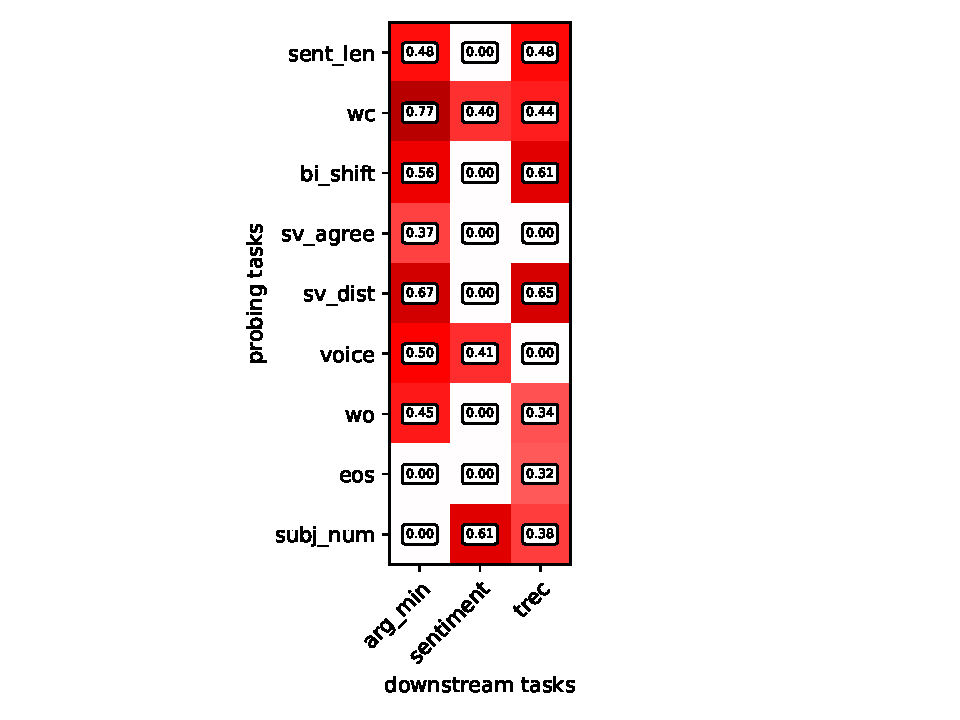
\includegraphics[scale=0.65]{images/spearman_corr_en_f1}
	\caption[Spearman correlations between probing and downstream task performances in English (F1 scores)]
		{Spearman correlations between probing and downstream task performances in English 
		\textbf{measured by F1 score}. \textcolor{red}{Reddish} values correspond to positive, \textcolor{blue}{blueish} values
		to negative correlations.}
	\label{fig:sp_corr_probing_downstream_en_f1}
\end{figure}

First of all, we notice that the correlations we obtained for the \caps{SentLen} task are rather high for \caps{TREC} and \caps{ArgMin}. This contradicts the finding reported by \citep{Conneau.2018a} who found that the \caps{SentLen} task is mainly negatively correlated with almost all downstream tasks (cf. figure \vref{fig:corr_conneau_perone}, left image). However, \citep{Eger.2019} have retrospectively correlated the results published by \citep{Perone.2018} and \textbf{found the exact opposite of what Conneau and colleagues report}. In this analysis, the \caps{SentLen} task shows the strongest connections to all downstream tasks on average (cf. figure \vref{fig:corr_conneau_perone}, right image). \citep{Eger.2019} conjecture that different sets of sentence embedding algorithms considered in the two papers are responsible for the divergence of the results. Conneau and colleagues use a set of related embeddings, whereas Perone et al. consider a more diverse set. \textbf{Different algorithms might focus on different linguistic aspects which influences the correlations.}

% Figure: Correlations by Conneau and Perone
\begin{figure}[h]
	\centering
	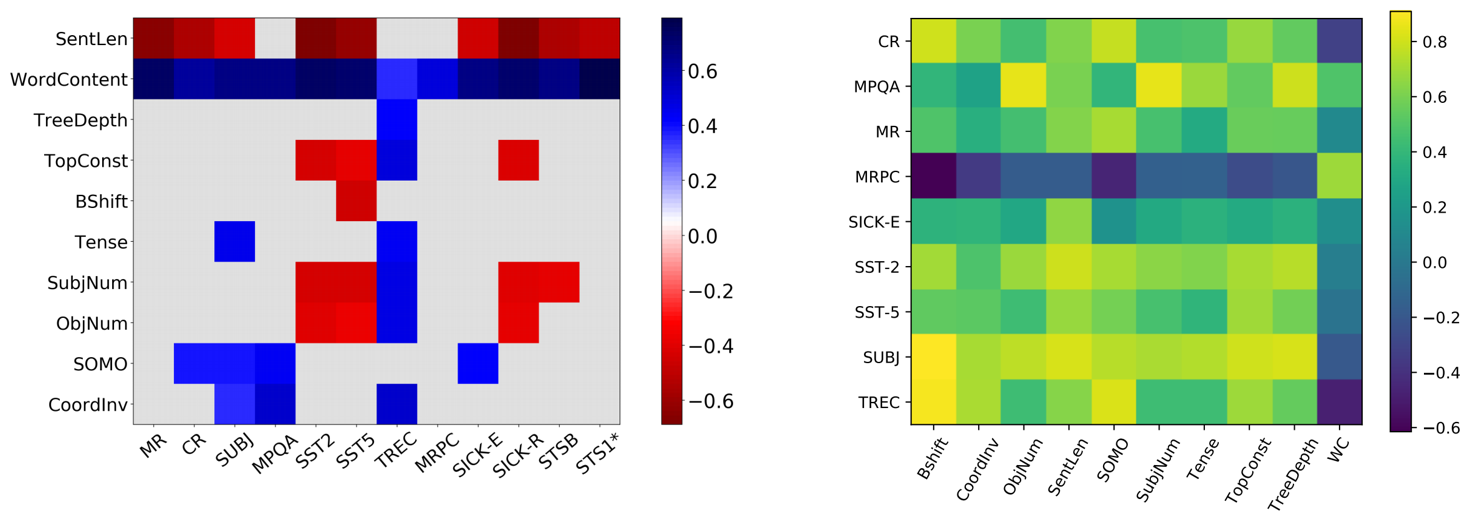
\includegraphics[scale=0.35]{images/corr_conneau_perone}
	\caption[Correlations between probing and downstream task performances from the literature]
		{Correlations between probing and downstream task performances from the literature.
		Left: Correlations reported by \citep{Conneau.2018a}. Please note that the color scheme is inverted.; 
		Right: Correlations of the results by \citep{Perone.2018}. The correlations were computed retrospectively by
		\citep{Eger.2019}.}
	\label{fig:corr_conneau_perone}
\end{figure}

% Table: Comparison of correlations with Krasnowska et al.
\begin{table}[h]
	\renewcommand{\arraystretch}{1.5}
	\centering
	\scalebox{1.0}{
	\begin{tabular}{ c c c c c c c c c c c c }
		\rotff{\textbf{Task}}							&
		\rotff{\textit{FastText\textsubscript{max}}} 		&
		\rotff{\textit{FastText\textsubscript{mean}}} 	&
		\rotff{\textit{BERT\textsubscript{max}}} 		&
		\rotff{\textit{BERT\textsubscript{mean}}} 		&
		\rotff{\textit{COMBO\textsubscript{max}}} 		&
		\rotff{\textit{COMBO\textsubscript{mean}}} 		&
		\rotff{\textit{sent2vec\textsubscript{ns}}} 		&
		\rotff{\textit{sent2vec\textsubscript{orig}}} 		&
		\rotff{\textit{LASER}} 						&
		\rotff{\textit{USE}} 							&
		\rotff{$\bm{r_s}$ \caps{Entail}}				\\
		\hline
		\textbf{\caps{SentLen}} 		& 52.55 & 72.27 & 72.66 & 82.13 & 85.03 & 87.38 & 71.56 & 64.76 & 85.98 & 60.00 
									& \textbf{-0.26} 	\\
		\hline
		\textbf{\caps{WC}} 			& 24.44 & 46.73 & 35.24 & 45.53 & 9.39 & 11.05 & 59.96 & 79.23 & 59.79 & 43.11
									& \textbf{0.72}	\\
		\hline
		\textbf{\caps{Voice}} 			& 84.13 & 89.47 & 89.77 & 92.40 & 98.48 & 98.41 & 88.73 & 89.04 & 92.85 & 86.61 
									& \textbf{-0.36}	\\
		\hline
		\textbf{\caps{SubjNum}}		& 73.87 & 81.43 & 88.43 & 90.75 & 93.19 & 93.37 & 82.27 & 80.88 & 94.21 & 81.65
									& \textbf{-0.02} 	\\
		\hline\hline
		\textbf{\caps{Entailment}}		& 76.72 & 76.86 & 77.71 & 77.11 & 72.82 & 72.58 & 78.59 & 78.26 & 83.26 & 81.77
									& -- \\
		\hline
	\end{tabular}}
	\caption[Results reported by Krasnowska et al. for several probing tasks as well as \caps{Entailment}]
		{Results reported by \citep{Krasnowska.2019} for several probing tasks as well as \caps{Entailment}.}
	\label{tab:comparison_correlation_krasnowska}
\end{table}

\textbf{Conneau and colleagues furthermore highlight the very strong positive correlations of the \caps{WC} task with all downstream applications.} This finding can be replicated in our experiment for the English language. This suggests that storing lexical information in the embeddings helps in downstream tasks. Consider for example the \caps{Senti} task, where the goal is to classify a sentence (or a snippet of text) into either positive or negative sentiment: If a sentence predominantly contains negatively (positively) connoted words, it is much more likely that this sentence also describes a negative (positive) sentiment. The \caps{ArgMin} task may serve as an additional example: The data set consists of sentences arguing either for or against a specific topic. If an embedding encodes information about argumentative words like e.\,g. \textit{`on the other hand'}, \textit{`likewise'}, \textit{`despite'}, \textit{`nevertheless'}, \textit{`as a consequence', etc.}, the classification of sentences into either supportive or confuting is accomplished much better. Finally, also the \caps{TREC} task profits from this knowledge: Storing information about the interrogative pronoun (question words like e.\,g. \textit{`what'}, \textit{`where'} and \textit{`how'}, etc.) directly gives hints as to what type of answer is expected. The results by \citep{Perone.2018}, on the other hand, indicate that knowledge about word containment is not as important for good performance in downstream applications \textbf{which sounds counter-intuitive}.

The correlations calculated by \citep{Conneau.2018a} furthermore indicate that detecting legal word orders is most of the time not indicative for good or bad performance in downstream applications. \textbf{Our results suggest a different conclusion:} The \caps{ArgMin} task as well as the \caps{TREC} task exhibit high correlations to the \caps{BiShift} probing task. This is compliant with the results by Perone et al. for which \citep{Eger.2019} compute a strong positive correlation of \caps{TREC} and \caps{BiShift}. We found that the closely related \caps{WO} task which also involves word order behaves analogously to \caps{BiShift}. \citep{Conneau.2018a} further point out that \textbf{the \caps{TREC} task has strong positive correlations with almost all probing tasks}. This finding can be reproduced in the context of our experiments. Only the tasks \caps{SVAgree} and \caps{Voice} are not connected to question type classification. Unfortunately, the \caps{SVAgree} task is not contained in the set of tasks introduced by Conneau et al., which is why a comparable figure is missing here.

\textbf{The \caps{Voice} task has positive correlations with the downstream tasks \caps{ArgMin} and \caps{Senti}}. If the accuracy metric is used (cf. figure \vref{fig:sp_corr_probing_downstream_en_acc}), the correlations become even stronger and \caps{Voice} is additionally correlated with \caps{TREC}. This suggests that voice information is helpful when it comes to performing well on downstream tasks. This finding is not intuitively obvious and the reasons for the importance of retaining voice information in sentence embeddings require further investigation. Unfortunately, this task is not included in the set of probing tasks shipped with \textit{SentEval}, but \citep{Krasnowska.2019} probed sentence embeddings using this task. The authors do not report probing task-downstream task correlations, but they report the accuracy values. Hence, it is possible to calculate the correlations retrospectively. The relevant results from their paper are summarized in table \vref{tab:comparison_correlation_krasnowska}. As can be seen from the table, the correlation between the probing task \caps{Voice} and the downstream task \caps{Entailment} is \textbf{negative}. \textbf{This means that \caps{Voice} is not always as predictive of downstream task performance as implied by the results we obtained.}

% Figure: Correlations between probing task / downstream task performance (en, accuracy)
\begin{figure}[h]
	\centering
	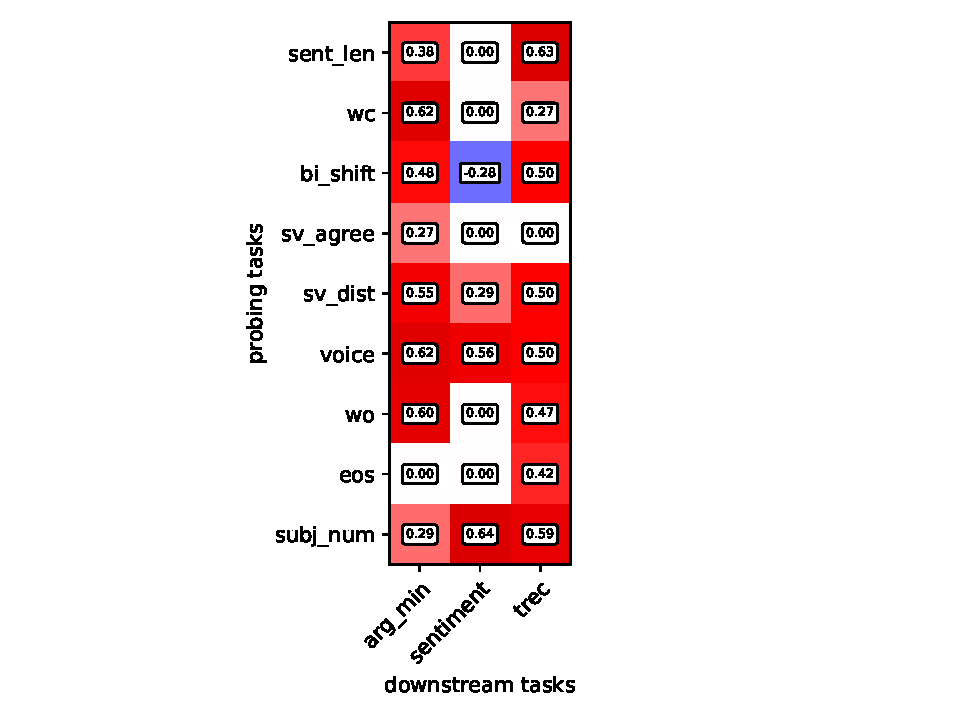
\includegraphics[scale=0.625]{images/spearman_corr_en_acc}
	\caption[Spearman correlations between probing and downstream task performances in English (accuracy)]
		{Spearman correlations between probing and downstream task performances in English 
		\textbf{measured by accuracy}. \textcolor{red}{Reddish} values correspond to positive, \textcolor{blue}{blueish} values
		to negative correlations.}
	\label{fig:sp_corr_probing_downstream_en_acc}
\end{figure}

\begin{tudbox}{Summary}
	\textbf{Many findings from the literature can be reproduced, yet differences can be observed due to different
	embeddings considered, different data sets or different probing and downstream tasks.}
\end{tudbox}

\highlight{Correlations in other languages.} The following paragraphs discuss the results for the remaining target languages, namely German, Russian, Turkish and Georgian. The figures \vref{fig:correlations_probing_downstream_de}, \vref{fig:correlations_probing_downstream_ru}, \vref{fig:correlations_probing_downstream_tr} and \vref{fig:correlations_probing_downstream_ka} show the respective results.

\textbf{The results for the other languages behave differently when compared to the English language.} In comparison to the English results, we notice first of all that a larger number of correlations is below an absolute value of 0.20, which is why they were set to 0.00. \textbf{What is more, many correlations have swapped into the negative range.} The strongest negative correlation can be observed for the Georgian \caps{WO} task, for which we computed a correlation with \caps{Senti} amounting to -0.73. Also the related \caps{BiShift} task shows a slight negative correlation with this downstream task in Georgian. The main reason for this may be the fact that it is possible to arrange words rather flexibly in the Georgian language (cf. section \vref{sec:georgian_language}), which renders the encoding of such information futile. Furthermore, an embedding has a finite number of dimensions. Encoding word order information might prevent the encoding of linguistic properties which are more relevant in the downstream tasks and might thus harm performance. While the \caps{TREC} task was reported to be correlated considerably positively with all probing tasks in the English language, \textbf{we could not reproduce this result in any of the other target languages}. The correlations for this task are either close to zero or negative. Furthermore, there are extremely strong positive correlations for the \caps{WC} task in German and less strong, but still noticeably positive correlations in Russian and Georgian. For the Turkish language we cannot confirm this finding: \textbf{There, the knowledge about word containment does not seem to be particularly decisive for downstream task performance}. This is surprising in light of the explanations given for the English language. In Turkish, the correlation between \caps{WC} and \caps{Senti} is even negative. This implies that either the explanations presented above are wrong, or they are at least not generalizable to all languages. Overall, the correlations in the Turkish language are less strong (except for the \caps{Senti} task with \caps{Voice} and \caps{SubjNum}). It is not entirely clear why this is the case for Turkish. 

% Figure: Correlations between probing task / downstream task performance (other languages: de, ru, tr, ka)
\begin{minipage}{0.49\textwidth}
	\begin{figure}[H]
		\centering
		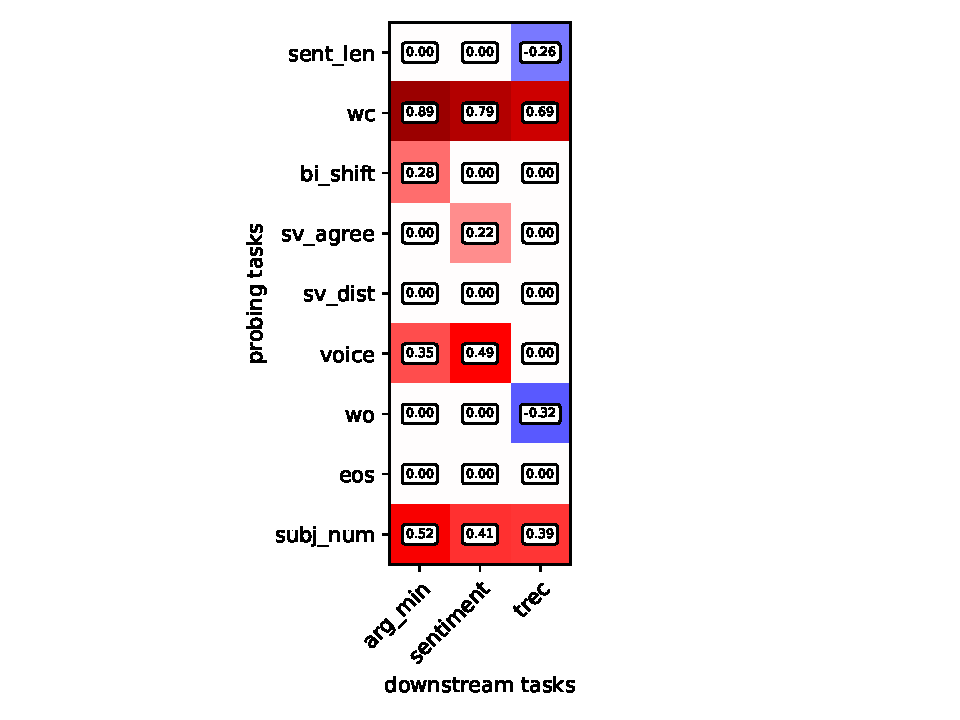
\includegraphics[scale=0.675]{images/spearman_corr_de_f1}
		\caption[Spearman correlations between probing and downstream task performances in German (F1 scores)]
			{Spearman correlations in German.}
		\label{fig:correlations_probing_downstream_de}
	\end{figure}
\end{minipage}
\hfill
\begin{minipage}{0.49\textwidth}
	\begin{figure}[H]
		\centering
		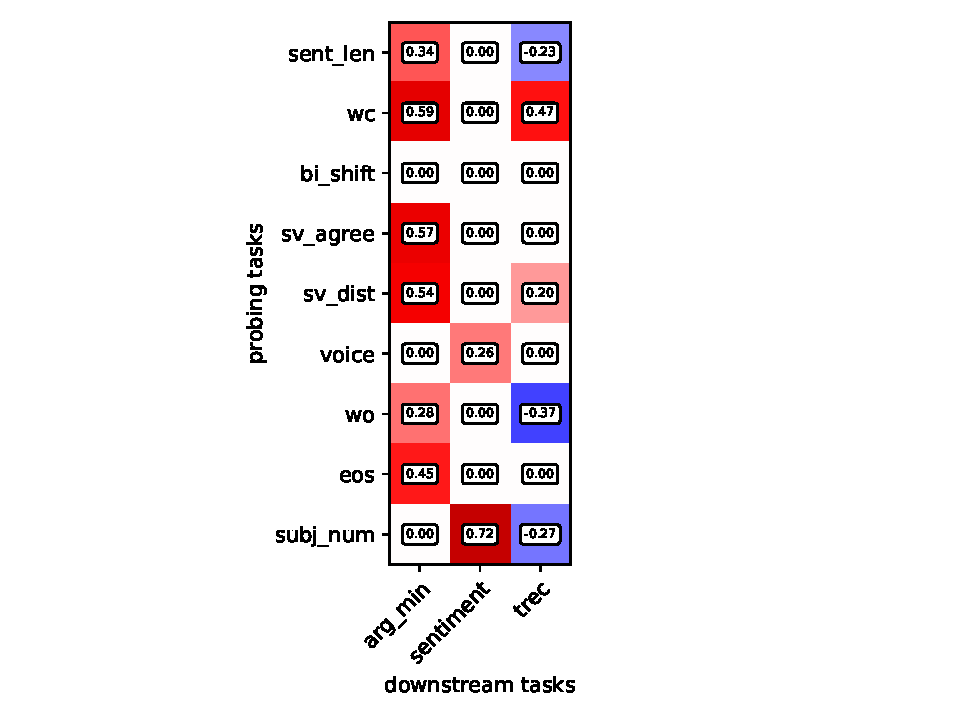
\includegraphics[scale=0.675]{images/spearman_corr_ru_f1}
		\caption[Spearman correlations between probing and downstream task performances in Russian (F1 scores)]
			{Spearman correlations in Russian.}
		\label{fig:correlations_probing_downstream_ru}
	\end{figure}
\end{minipage}

% Figure: Correlations between probing task / downstream task performance (other languages: de, ru, tr, ka)
\begin{minipage}{0.49\textwidth}
	\begin{figure}[H]
		\centering
		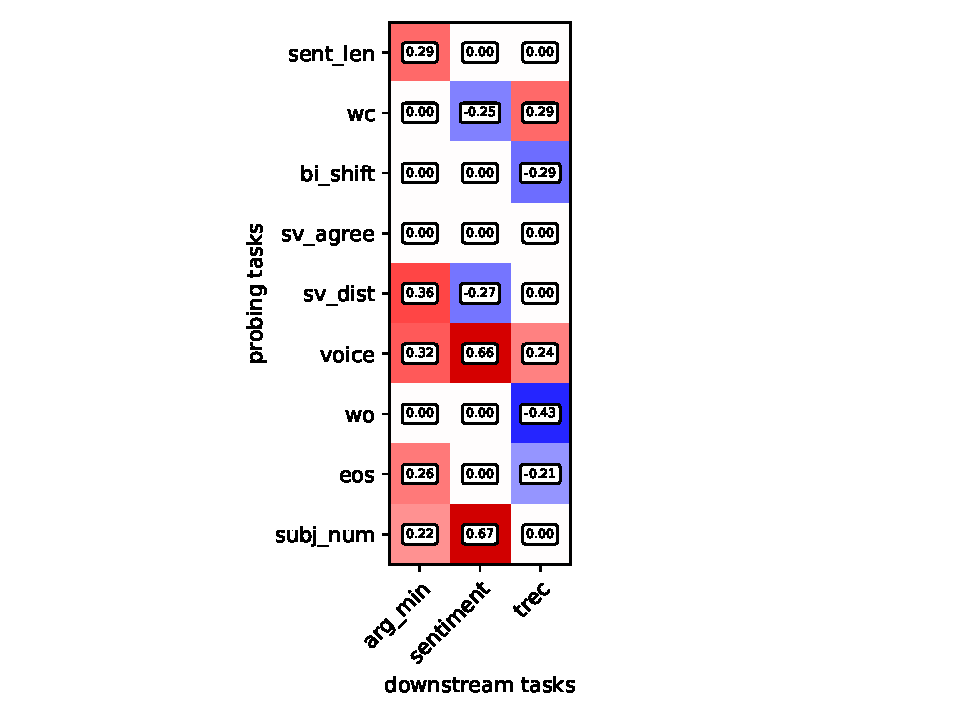
\includegraphics[scale=0.675]{images/spearman_corr_tr_f1}
		\caption[Spearman correlations between probing and downstream task performances in Turkish (F1 scores)]
			{Spearman correlations in Turkish.}
		\label{fig:correlations_probing_downstream_tr}
	\end{figure}
\end{minipage}
\hfill
\begin{minipage}{0.49\textwidth}
	\begin{figure}[H]
		\centering
		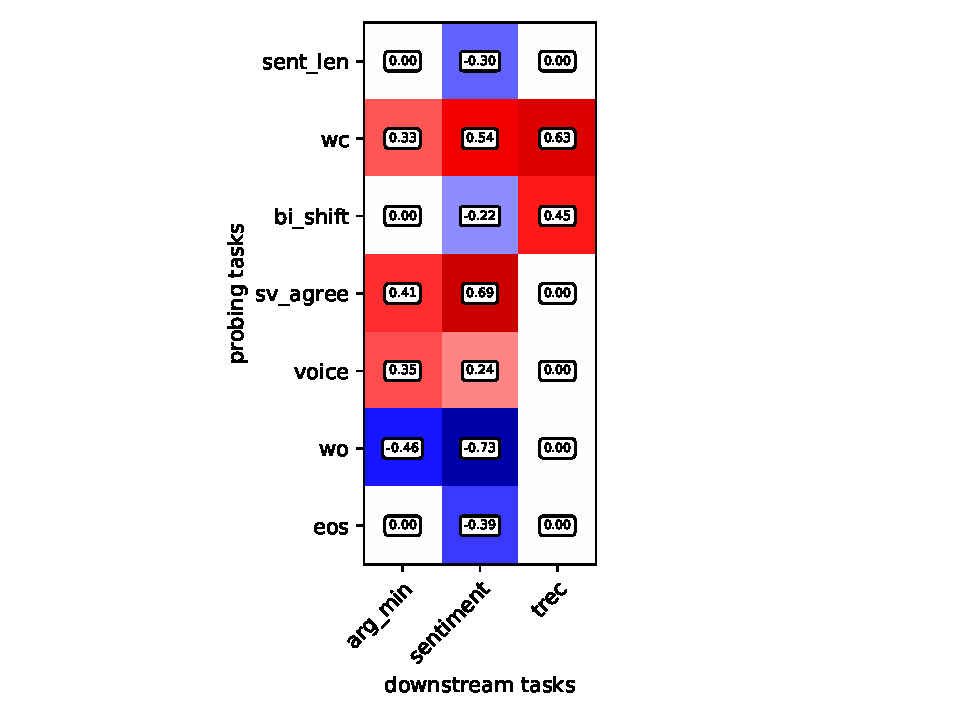
\includegraphics[scale=0.675]{images/spearman_corr_ka_f1}
		\caption[Spearman correlations between probing and downstream task performances in Georgian (F1 scores)]
			{Spearman correlations in Georgian.}
		\label{fig:correlations_probing_downstream_ka}
	\end{figure}
\end{minipage}

\vspace*{2mm}
\begin{tudbox}{Summary}
	\textbf{The results for the remaining languages are different compared to English. Many correlations have fallen below an absolute value of 0.20 or have swapped into the negative range entirely. The strongest negative correlation can be observed for the Georgian language. Also the correlations of the \caps{TREC} task with the set of probing tasks vanish. Turkish is the only language for which the knowledge about word containment is not predictive for downstream task performance.}
\end{tudbox}

\newpage
% -----------------------------------------------------------------------------------------------------------------------------------------------------
% Stability Analysis of the Embedding Ordering
\subsection{Stability Analysis of the Embedding Ordering}
\label{sec:stability_analysis}

One common problem in the evaluation of sentence embeddings on probing tasks is that different evaluation settings are used quite frequently. These differences are manifold: First of all, the size of the data sets are not standardized and vary as a consequence. Secondly, the research community did not agree on a single classifier type which is used to test the embeddings. Sometimes neural networks with a hidden layer are used, but also logistic regression is quite common. These two approaches differ in their representational power, thus influencing the final results. Furthermore, we detected settings where hyper-parameters like the number of hidden units or the dropout rate of an \gls{mlp} are tuned \citep{Conneau.2018a}, others use a fixed model architecture for the evaluation and do not mention hyper-parameter tuning explicitly \citep{Perone.2018}. I.\,e. it remains unclear whether or not they performed hyper-parameter optimization; and even if they did, they did not specify which hyper-parameters were tuned. Finally, the balance of the classes may have an influence on the performance of individual embeddings. On the one hand, \citep{Shi.2016} used an imbalanced \caps{Voice} data set for the evaluation (majority class amounts to 82.8\,\% for active voice), whereas, on the other hand, \citep{Conneau.2018a} created balanced data sets within the \textit{SentEval} framework. The data sets in this work are partially imbalanced (cf. tables \vref{tab:class_dist_probing_en_de}, \vref{tab:class_dist_probing_ru_tr} and \vref{tab:class_dist_probing_ka}), where especially the tasks \caps{SentLen} and \caps{WC} are concerned.

\textbf{These different setups motivated a detailed \textit{`stability analysis'} whose goal is \ding{182} to investigate the reasons for different results in this work and the literature, and \ding{183} to see which of the above mentioned factors have an influence on the ordering of the embeddings.} A review of the literature revealed that such a comprehensive study has not been conducted before. The following lines describe the experimental setup in greater depth: The analysis is performed for English and partially for Georgian using the example of the \caps{WC} task. The idea is to systematically change the factors of the evaluation setting one at a time (\textit{ceteris paribus}), such that the individual effects can be recorded. For reasons of time, it was not possible to perform this analysis exhaustively for all factor combinations. Instead, some combinations were picked and analyzed. The factors are as follows: \texttt{size} of the data set, \texttt{classifier}, \texttt{class balance} and \texttt{hyper-parameter tuning}.

\highlight{Factors \texttt{size} and \texttt{classifier}.} The first two factors which we investigate are \texttt{size} and \texttt{classifier}: We began by creating data sets of varying sizes for the \caps{WC} task. Since data sets which are too large require an excessive amount of computational resources, we decided to limit the size to a maximum of 60k instances. Four different data sets were created comprising 5k, 10k, 30k and 60k instances, respectively. The data sets were generated, such that data sets of smaller sizes are real subsets of larger data sets. \textbf{This entails that the 10k \caps{WC} task data set is not identical to the one used in earlier experiments. Hence, minor deviations in performance must be expected as a consequence.} The investigation of \texttt{classifier} effects requires that a set of diverse classification algorithms be chosen. To this end, we browsed the \textit{scikit-learn} library for adequate classifiers. The list below shows the classifiers which were used and also gives information with respect to the hyper-parameters used in the experiments:

\begin{tabbing}
	\hspace*{1cm}\=\hspace*{4cm}\=\hspace*{6cm}\=\kill
		\>	\textbf{Hyper-parameter}
		\>	\textbf{Argument}
		\>	\textbf{Explanation} 	\\[4mm]
	\ding{182} \textbf{Logistic regression (\texttt{LR})} 
		\>	\>	\> 	
\includegraphics[scale=0.02]{images/sklearn}									\\[3mm]
		\>	\texttt{C}			\>	3.75					\>	Regularization parameter			\\[3mm]
		\> 	\texttt{solver}		\>	lbfgs					\>	Optimization technique			\\[3mm]
		\>	\texttt{multi\_class}	\>	multinomial				\>	Multi-class setting					\\[4mm]
	\ding{183} \textbf{Random forest (\texttt{RF})}
		\>	\>	\> 	
\includegraphics[scale=0.02]{images/sklearn}									\\[3mm]
		\>	\texttt{n\_estimators}	\>	250						\>	Number of trees in the ensemble	\\[3mm]
		\>	\texttt{criterion} 		\>	gini						\>	Splitting heuristic					\\[3mm]
		\>	\texttt{max\_depth}	\>	70						\>	Maximum depth of single tree		\\[4mm]
	\ding{184} \textbf{Gaussian na\"{i}ve bayes (\texttt{NB})} 
		\>	\>	\> 	
\includegraphics[scale=0.02]{images/sklearn}									\\[3mm]
		\> 	no hyper-parameters 	\>							\>									\\[4mm]
	\ding{185} \textbf{Support vector machine (\texttt{SVM})}
		\>	\>	\> 	
\includegraphics[scale=0.02]{images/sklearn}									\\[3mm]
		\>	\texttt{kernel}		\>	linear					\>	Kernel type						\\[3mm]
		\>	\texttt{C}			\>	3.0						\>	Regularization parameter	\\[4mm]
	\ding{186} \textbf{Neural network without hidden layer (\texttt{NN})}
		\>	\>	\> 	
\includegraphics[scale=0.025]{images/keras}									\\[3mm]
		\>	\texttt{n\_epochs}	\>	100						\>	Number of training epochs			\\[3mm]
		\>	\texttt{loss} 			\>	categorical cross-entropy	\>	loss function							\\[3mm]
		\> 	\texttt{optimizer}		\> 	adam					\>	Optimization technique			\\[3mm]
		\> 	\texttt{act\_func} 	\>	sigmoid					\>	Activation function				\\[4mm]
	\ding{187} \textbf{Neural network with hidden layer (\texttt{NN\_H})}
		\>	\>	\> 	
\includegraphics[scale=0.025]{images/keras}									\\[3mm]
		\> 	\texttt{n\_hidden}	\>	50						\>	Number of neurons in hidden layer	\\[3mm]
		\> 	\texttt{drop\_out}	\>	0.00					\>	Dropout rate					\\[3mm]
		\> 	\textit{Other arguments equal to \texttt{NN}}\>		\>									\\
\end{tabbing}

These hyper-parameters were kept fixed for the factors \texttt{size} and \texttt{classifier} in the first half of this experiment. In order to obtain more stable results, we furthermore repeated the experiment, such that three individual results were available. The numbers listed in the following tables were produced by averaging the results over these three runs. Within each run we ensured that \textbf{all classifiers are evaluated on the same train-test splits across all embeddings} using an approach called \textbf{random subset evaluation}. Also, the random states of the classifiers were set, such that e.\,g. different weight initializations (for neural networks) or different attribute subset selections (for random forests) do not influence the results. \textbf{NB:} Results for the \gls{svm} classifier were produced only for 5k and 10k instances due to excessive computation time.

Table \vref{tab:corr_wc_en_clfs} shows the Spearman correlations obtained on the \caps{WC} task by using different \texttt{classifier}s, whereas table \vref{tab:corr_wc_en_sizes} focuses on correlations between varying data set \texttt{size}s. This evaluation serves two purposes: \ding{182} \textbf{Firstly, it is possible to determine a data set size for which no more considerable changes in the ranking of the embeddings take place.} \ding{183} \textbf{Secondly, the experiment allows for conclusions with respect to the rank stability of the embeddings across different classifiers.} We omitted detailed results here. In depth test results can be found in appendix \vref{sec:appendix_stability_analysis}).

% Figure: correlations word content English (10,000 instances, different classifiers)
\begin{table}[h]
	\centering
	\renewcommand{\arraystretch}{1.1}
	\scalebox{1.1}{
	\begin{tabular}{| l || c | c | c | c | c | c |}
		\hline
		\rowcolor{tud9c!50}
		\multicolumn{7}{| c |}{\textbf{10k instances (EN)}}		\\ \hline\hline
		\textbf{\texttt{LR}}		& 1.00 	& \gr 	& \gr 	& \gr	& \gr 	& \gr 	\\ \hline
		\textbf{\texttt{NN}}		& 0.91 	& 1.00 	& \gr 	& \gr	& \gr 	& \gr	\\ \hline
		\textbf{\texttt{NN\_H}}	& 0.83	& 0.94	& 1.00 	& \gr 	& \gr 	& \gr	\\ \hline
		\textbf{\texttt{RF}}		& 0.41	& 0.66	& 0.81	& 1.00 	& \gr 	& \gr	\\ \hline
		\textbf{\texttt{SVM}}		& 0.85	& 0.90	& 0.94	& 0.76	& 1.00 	& \gr	\\ \hline
		\textbf{\texttt{NB}}		& 0.84	& 0.83	& 0.76	& 0.34	& 0.78	& 1.00	\\ \hline\hline
		& \textbf{\texttt{LR}} & \textbf{\texttt{NN}} & \textbf{\texttt{NN\_H}} & \textbf{\texttt{RF}} & \textbf{\texttt{SVM}}
		& \textbf{\texttt{NB}} \\ \hline
	\end{tabular}}
	\caption[Spearman correlations for different classifiers (\caps{WC} task, EN, 10k instances)]
		{Spearman correlations computed for different classifiers (\caps{WC} task, EN, 10k instances).}
	\label{tab:corr_wc_en_clfs}
\end{table}

First of all consider the results reported in table \vref{tab:corr_wc_en_clfs} which shows the Spearman correlations of the embedding ordering when different classifiers are employed. The numbers in the table were produced on a fixed-sized data set comprising 10k instances. When looking at the numbers, we realize immediately that \textbf{the ordering of the embeddings is in general rather unstable across different classifiers} (correlations move in the range from 0.34 to 0.94). This holds especially true for the \texttt{RF} classifier for which the correlations deviate drastically from the remaining classifiers. We can reproduce this finding on the 5k, 30k and 60k data sets (cf. appendix \vref{sec:appendix_stability_analysis} for more information). Consistent lower correlations can also be observed for \texttt{NB}. Our experiments also show that neural architectures outperform the \texttt{RF} classifier and \texttt{NB}. For \textit{InferSent} embeddings on 60k instances we observed the following differences in performance: $\Delta$ \texttt{NN\_H} $\leftrightarrow$ \texttt{RF}/\texttt{NB} +0.21/+0.41 F1 score. (cf. table \vref{tab:results_en_wc_60000}). As expected, the correlation between the \texttt{LR} classifier and \texttt{NN} is noticeably positive, since both models are closely related. Also the positive correlation between the two neural architectures (\texttt{NN\_H} and \texttt{NN}) is considerable. \textbf{In summary, our results suggest that the choice of a specific classifier cannot be made blindly. Furthermore, classifiers like \texttt{NB} or \texttt{RF} should not be used, since they are consistently outperformed by neural architectures or logistic regression in our experiments.}

% Figure: correlations word content English (per classifier, different sizes)
\begin{table}[h]
	\begin{minipage}{0.32\textwidth}
		\begin{table}[H]
	\centering
	\scalebox{0.8}{
	\begin{tabular}{| l || c | c | c | c |}
		\hline
		\rowcolor{tud9c!50}
		\multicolumn{5}{| c |}{\textbf{\texttt{LR} classifier (EN)}}
		\\ \hline\hline
		\textbf{5k}		& 1.00 	& \gr 	& \gr 	& \gr 				\\ \hline
		\textbf{10k}		& 0.99 	& 1.00 	& \gr 	& \gr				\\ \hline
		\textbf{30k}		& 0.93	& 0.94	& 1.00 	& \gr 				\\ \hline
		\textbf{60k}		& 0.90	& 0.92	& 0.99	& 1.00				\\ \hline\hline
		& \textbf{5k} & \textbf{10k} & \textbf{30k} & \textbf{60k} 		\\ \hline
	\end{tabular}}
\end{table}
	\end{minipage}
	\hfill
	\begin{minipage}{0.32\textwidth}
		\begin{table}[H]
	\centering
	\scalebox{0.8}{
	\begin{tabular}{| l || c | c | c | c |}
		\hline
		\rowcolor{tud9c!50}
		\multicolumn{5}{| c |}{\textbf{\texttt{NN} classifier (EN)}}
		\\ \hline\hline
		\textbf{5k}		& 1.00 	& \gr 	& \gr 	& \gr 				\\ \hline
		\textbf{10k}		& 0.98 	& 1.00 	& \gr 	& \gr				\\ \hline
		\textbf{30k}		& 0.90	& 0.96	& 1.00 	& \gr 				\\ \hline
		\textbf{60k}		& 0.88	& 0.94	& 0.99	& 1.00				\\ \hline\hline
		& \textbf{5k} & \textbf{10k} & \textbf{30k} & \textbf{60k} 		\\ \hline
	\end{tabular}}
\end{table}
	\end{minipage}
	\hfill
	\begin{minipage}{0.32\textwidth}
		\begin{table}[H]
	\centering
	\scalebox{0.8}{
	\begin{tabular}{| l || c | c | c | c |}
		\hline
		\rowcolor{tud9c!50}
		\multicolumn{5}{| c |}{\textbf{\texttt{NN\_H} classifier (EN)}}
		\\ \hline\hline
		\textbf{5k}		& 1.00 	& \gr 	& \gr 	& \gr 				\\ \hline
		\textbf{10k}		& 0.95 	& 1.00 	& \gr 	& \gr				\\ \hline
		\textbf{30k}		& 0.87	& 0.94	& 1.00 	& \gr 				\\ \hline
		\textbf{60k}		& 0.84	& 0.92	& 0.99	& 1.00				\\ \hline\hline
		& \textbf{5k} & \textbf{10k} & \textbf{30k} & \textbf{60k} 		\\ \hline
	\end{tabular}}
\end{table}
	\end{minipage}

	\begin{minipage}{0.49\textwidth}
		\begin{table}[H]
	\centering
	\scalebox{0.8}{
	\begin{tabular}{| l || c | c | c | c |}
		\hline
		\rowcolor{tud9c!50}
		\multicolumn{5}{| c |}{\textbf{\texttt{RF} classifier (EN)}}
		\\ \hline\hline
		\textbf{5k}		& 1.00 	& \gr 	& \gr 	& \gr 				\\ \hline
		\textbf{10k}		& 0.99 	& 1.00 	& \gr 	& \gr				\\ \hline
		\textbf{30k}		& 0.97	& 0.97	& 1.00 	& \gr 				\\ \hline
		\textbf{60k}		& 0.97	& 0.97	& 1.00	& 1.00				\\ \hline\hline
		& \textbf{5k} & \textbf{10k} & \textbf{30k} & \textbf{60k} 		\\ \hline
	\end{tabular}}
\end{table}
	\end{minipage}
	\hfill
	\begin{minipage}{0.49\textwidth}
		\begin{table}[H]
	\centering
	\scalebox{0.8}{
	\begin{tabular}{| l || c | c | c | c |}
		\hline
		\rowcolor{tud9c!50}
		\multicolumn{5}{| c |}{\textbf{\texttt{NB} classifier (EN)}}
		\\ \hline\hline
		\textbf{5k}		& 1.00 	& \gr 	& \gr 	& \gr 				\\ \hline
		\textbf{10k}		& 1.00 	& 1.00 	& \gr 	& \gr				\\ \hline
		\textbf{30k}		& 0.94	& 0.94	& 1.00 	& \gr 				\\ \hline
		\textbf{60k}		& 0.92	& 0.92	& 0.99	& 1.00				\\ \hline\hline
		& \textbf{5k} & \textbf{10k} & \textbf{30k} & \textbf{60k} 		\\ \hline
	\end{tabular}}
\end{table}
	\end{minipage}
	\caption[Spearman correlations per classifier for different data set sizes (\caps{WC} task, EN)]
		{Spearman correlations per classifier computed for different data set sizes (\caps{WC} task, EN).}
	\label{tab:corr_wc_en_sizes}
\end{table}

Table \vref{tab:corr_wc_en_sizes} presents the rank stability with different data set sizes. We notice that for most of the classifiers, \textbf{the relative rankings between the embeddings change substantially between 5k training examples and a training set size of 60k instances}. Consider for example the numbers computed for the \texttt{NN\_H} classifier (top right), where the Spearman correlation between 5k and 60k instances amounting to 0.84 is rather low. At the same time, the correlation between 30k and 60k training examples is very close to 1.0 (also for the remaining classifiers). This means that the additional 30k training examples do not entail any noticeable changes in the ordering of the embeddings. \textbf{We therefore conclude that a data set size of 30k instances is sufficient to obtain a stable embedding ordering (at least on the \caps{WC} task in the English language).} For the \texttt{RF} classifier (bottom left), the correlations are already quite high between 5k and 60k training examples. \textbf{This means, that the ordering of the embeddings using this classifier is already relatively stable, even when training on small data sets.}

% Table: Embedding Ordering for 60,000 instances
\begin{table}[h]
	\centering
	\renewcommand{\arraystretch}{1.5}
	\scalebox{0.75}{
	\begin{tabularx}{1.3\textwidth}{| X ? Y | c ? Y | c ? Y | c ? Y | c ? Y | c |}
		\rowcolor{tud9c}
		\hline
																	&
		\multicolumn{2}{ c ?}{\textcolor{white}{\textbf{\texttt{LR}}}}	&
		\multicolumn{2}{ c ?}{\textcolor{white}{\textbf{\texttt{NN}}}	}	&
		\multicolumn{2}{ c ?}{\textcolor{white}{\textbf{\texttt{NN\_H}}}}&
		\multicolumn{2}{ c ?}{\textcolor{white}{\textbf{\texttt{RF}}}}	&
		\multicolumn{2}{ c |}{\textcolor{white}{\textbf{\texttt{NB}}}}	\\
		\multirow{-2}{*}{
			\cellcolor{tud9c}{\textcolor{white}{\textbf{60k instances}}}} 	&
		\cellcolor{tud9c!70}\textbf{F1} & \cellcolor{tud9c!70}\textbf{R} 	&
		\cellcolor{tud9c!70}\textbf{F1} & \cellcolor{tud9c!70}\textbf{R} 	&
		\cellcolor{tud9c!70}\textbf{F1} & \cellcolor{tud9c!70}\textbf{R} 	&
		\cellcolor{tud9c!70}\textbf{F1} & \cellcolor{tud9c!70}\textbf{R} 	&
		\cellcolor{tud9c!70}\textbf{F1} & \cellcolor{tud9c!70}\textbf{R} 	\\ \hline\hline

		Vanilla Average 	& 0.66 & 6 	& 0.78 & 8 	& 0.81 & 6 	& 0.31 & 9 	& 0.38 & 7 	\\ \hline
		GEM 			& 0.81 & 5 	& 0.81 & 5 	& 0.78 & 8 	& 0.36 & 8 	& 0.48 & 5 	\\ \hline
		SIF 				& 0.65 & 7 	& 0.79 & 7 	& 0.81 & 7 	& 0.38 & 7 	& 0.43 & 6 	\\ \hline
		p-Means 		& 0.45 & 10 	& 0.80 & 6 	& 0.82 & 4 	& 0.45 & 5 	& 0.23 & 9 	\\ \hline
		hier. pooling 		& 0.45 & 9 	& 0.51 & 12 	& 0.52 & 12 	& 0.24 & 11 	& 0.21 & 10	\\ \hline
		BOREP 			& 0.40 & 11 	& 0.66 & 10 	& 0.67 & 10 	& 0.59 & 3 	& 0.15 & 12	\\ \hline
		Random BiLSTM 	& 0.36 & 12 	& 0.68 & 9 	& 0.75 & 9 	& 0.30 & 10 	& 0.16 & 11	\\ \hline
		sent2vec 		& 0.83 & 4 	& 0.82 & 4 	& 0.81 & 5 	& 0.39 & 6 	& 0.64 & 1	\\ \hline
		Quick-Thought 	& 0.86 & 3 	& 0.92 & 2 	& 0.91 & 3 	& 0.57 & 4 	& 0.50 & 4	\\ \hline
		LASER 			& 0.88 & 2 	& 0.91 & 3 	& 0.92 & 2 	& 0.72 & 2 	& 0.55 & 3	\\ \hline
		BERT 			& 0.57 & 8 	& 0.59 & 11 	& 0.57 & 11 	& 0.22 & 12 	& 0.27 & 8	\\ \hline
		InferSent 		& 0.96 & 1 	& 0.97 & 1 	& 0.98 & 1 	& 0.77 & 1 	& 0.57 & 2	\\ \hline
	\end{tabularx}}
	\caption[Stability analysis results for 60k instances (\caps{WC} task, EN)]
		{Stability analysis results for 60k instances in (\caps{WC} task, EN).}
	\label{tab:results_en_wc_60000}
\end{table}

Table \vref{tab:results_en_wc_60000} shows detailed results of the embedding performances on the 60k data set: We see that the numbers for some of the embeddings are still not in the range reported by \citep{Perone.2018,Conneau.2018a}. Consider for instance the \textit{vanilla average} embedding for which Conneau and colleagues report 91.60\,\% accuracy on the \caps{WC} task. The result for the \texttt{NN\_H} classifier listed above (0.81) indicates that this still outperforms our score (the table shows F1 scores, the respective accuracy score on the data set is 86.31\,\%), although there are less classes in our setup. \textbf{Our results further suggest that the neural network without hidden layer (\texttt{NN}) performs worse than the \gls{mlp} (\texttt{NN\_H}).} \citep{Perone.2018,Conneau.2018a} removed the hidden layer for the evaluation on the \caps{WC} task because this gave better results in their experiments.\footnote{\citep{Conneau.2018a} refer to the \texttt{NN} classifier as logistic regression. This implementation must not be confused with \texttt{LR} which we adopted from the \textit{scikit-learn} library.} We were unable to observe this effect in our results. As table \vref{tab:results_en_wc_60000} reveals, the \texttt{NN} classifier is outperformed by the \texttt{NN\_H} classifier for 8 out of 12 embeddings. \textbf{The overall results suggest that the size of the data set as well as the classifier architecture are not the only effects to be made responsible for the deviations.} Before we examine the effects of the other factors (\texttt{class balance} and \texttt{hyper-parameter tuning}), we want to investigate whether the findings above can be reproduced for the Georgian language. In this context, the following results were obtained:

% Figure: correlations word content Georgian (10,000 instances, different classifiers)
\begin{table}[h]
	\centering
	\renewcommand{\arraystretch}{1.1}
	\scalebox{1.1}{
	\begin{tabular}{| l || c | c | c | c | c | c |}
		\hline
		\rowcolor{tud9c!50}
		\multicolumn{7}{| c |}{\textbf{10k instances (KA)}}		\\ \hline\hline
		\textbf{\texttt{LR}}		& 1.00 	& \gr 	& \gr 	& \gr	& \gr 	& \gr 	\\ \hline
		\textbf{\texttt{NN}}		& 0.88 	& 1.00 	& \gr 	& \gr	& \gr 	& \gr	\\ \hline
		\textbf{\texttt{NN\_H}}	& 0.89	& 0.98	& 1.00 	& \gr 	& \gr 	& \gr	\\ \hline
		\textbf{\texttt{RF}}		& 0.45	& 0.49	& 0.62	& 1.00 	& \gr 	& \gr	\\ \hline
		\textbf{\texttt{SVM}}		& 0.99	& 0.90	& 0.92	& 0.50	& 1.00 	& \gr	\\ \hline
		\textbf{\texttt{NB}}		& 0.61	& 0.76	& 0.71	& 0.13	& 0.60	& 1.00	\\ \hline\hline
		& \textbf{\texttt{LR}} & \textbf{\texttt{NN}} & \textbf{\texttt{NN\_H}} & \textbf{\texttt{RF}} & \textbf{\texttt{SVM}}
		& \textbf{\texttt{NB}} \\ \hline
	\end{tabular}}
	\caption[Spearman correlations for different classifiers (\caps{WC} task, KA, 10k instances)]
		{Spearman correlations computed for different classifiers (\caps{WC} task, KA, 10k instances).}
	\label{tab:corr_wc_ka_clfs}
\end{table}

% Figure: correlations word content Georgian (per classifier, different sizes)
\begin{table}[h]
	\begin{minipage}{0.32\textwidth}
		\begin{table}[H]
	\centering
	\scalebox{0.8}{
	\begin{tabular}{| l || c | c | c | c |}
		\hline
		\rowcolor{tud9c!50}
		\multicolumn{5}{| c |}{\textbf{\texttt{LR} classifier (KA)}}
		\\ \hline\hline
		\textbf{5k}		& 1.00 	& \gr 	& \gr 	& \gr 				\\ \hline
		\textbf{10k}		& 0.94 	& 1.00 	& \gr 	& \gr				\\ \hline
		\textbf{30k}		& 0.93	& 0.96	& 1.00 	& \gr 				\\ \hline
		\textbf{60k}		& 0.91	& 0.95	& 0.99	& 1.00				\\ \hline\hline
		& \textbf{5k} & \textbf{10k} & \textbf{30k} & \textbf{60k} 		\\ \hline
	\end{tabular}}
\end{table}
	\end{minipage}
	\hfill
	\begin{minipage}{0.32\textwidth}
		\begin{table}[H]
	\centering
	\scalebox{0.8}{
	\begin{tabular}{| l || c | c | c | c |}
		\hline
		\rowcolor{tud9c!50}
		\multicolumn{5}{| c |}{\textbf{\texttt{NN} classifier (KA)}}
		\\ \hline\hline
		\textbf{5k}		& 1.00 	& \gr 	& \gr 	& \gr 				\\ \hline
		\textbf{10k}		& 0.97 	& 1.00 	& \gr 	& \gr				\\ \hline
		\textbf{30k}		& 0.88	& 0.93	& 1.00 	& \gr 				\\ \hline
		\textbf{60k}		& 0.85	& 0.88	& 0.98	& 1.00				\\ \hline\hline
		& \textbf{5k} & \textbf{10k} & \textbf{30k} & \textbf{60k} 		\\ \hline
	\end{tabular}}
\end{table}
	\end{minipage}
	\hfill
	\begin{minipage}{0.32\textwidth}
		\begin{table}[H]
	\centering
	\scalebox{0.8}{
	\begin{tabular}{| l || c | c | c | c |}
		\hline
		\rowcolor{tud9c!50}
		\multicolumn{5}{| c |}{\textbf{\texttt{NN\_H} classifier (KA)}}
		\\ \hline\hline
		\textbf{5k}		& 1.00 	& \gr 	& \gr 	& \gr 				\\ \hline
		\textbf{10k}		& 0.99 	& 1.00 	& \gr 	& \gr				\\ \hline
		\textbf{30k}		& 0.87	& 0.91	& 1.00 	& \gr 				\\ \hline
		\textbf{60k}		& 0.72	& 0.77	& 0.94	& 1.00				\\ \hline\hline
		& \textbf{5k} & \textbf{10k} & \textbf{30k} & \textbf{60k} 		\\ \hline
	\end{tabular}}
\end{table}
	\end{minipage}

	\begin{minipage}{0.49\textwidth}
		\begin{table}[H]
	\centering
	\scalebox{0.8}{
	\begin{tabular}{| l || c | c | c | c |}
		\hline
		\rowcolor{tud9c!50}
		\multicolumn{5}{| c |}{\textbf{\texttt{RF} classifier (KA)}}
		\\ \hline\hline
		\textbf{5k}		& 1.00 	& \gr 	& \gr 	& \gr 				\\ \hline
		\textbf{10k}		& 0.99 	& 1.00 	& \gr 	& \gr				\\ \hline
		\textbf{30k}		& 0.97	& 0.97	& 1.00 	& \gr 				\\ \hline
		\textbf{60k}		& 0.97	& 0.97	& 1.00	& 1.00				\\ \hline\hline
		& \textbf{5k} & \textbf{10k} & \textbf{30k} & \textbf{60k} 		\\ \hline
	\end{tabular}}
\end{table}
	\end{minipage}
	\hfill
	\begin{minipage}{0.49\textwidth}
		\begin{table}[H]
	\centering
	\scalebox{0.8}{
	\begin{tabular}{| l || c | c | c | c |}
		\hline
		\rowcolor{tud9c!50}
		\multicolumn{5}{| c |}{\textbf{\texttt{NB} classifier (KA)}}
		\\ \hline\hline
		\textbf{5k}		& 1.00 	& \gr 	& \gr 	& \gr 				\\ \hline
		\textbf{10k}		& 0.94 	& 1.00 	& \gr 	& \gr				\\ \hline
		\textbf{30k}		& 0.95	& 0.98	& 1.00 	& \gr 				\\ \hline
		\textbf{60k}		& 0.97	& 0.99	& 0.99	& 1.00				\\ \hline\hline
		& \textbf{5k} & \textbf{10k} & \textbf{30k} & \textbf{60k} 		\\ \hline
	\end{tabular}}
\end{table}
	\end{minipage}
	\caption[Spearman correlations per classifier for different data set sizes (\caps{WC} task, KA)]
		{Spearman correlations per classifier computed for different data set sizes (\caps{WC} task, KA).}
	\label{tab:corr_wc_ka_sizes}
\end{table}

\textbf{Overall, the analysis of the embedding orderings using different classifiers yields a similar picture for Georgian compared to the English language} (cf. table \vref{tab:corr_wc_ka_clfs}): The \texttt{RF} classifier still exhibits the lowest correlation to all other classifiers. We observe the lowest correlation between \texttt{RF} and \texttt{NB} (0.13). Table \vref{tab:corr_wc_ka_sizes} furthermore confirms that \textbf{a data set size of approximately 30k instances is sufficient} in order to obtain a stable embedding ordering. Only the correlation between the sizes 30k and 60k for the \texttt{NN\_H} classifier amounts to a slightly smaller number (0.94) compared to English (cf. table \vref{tab:corr_wc_en_sizes}). An interesting observation is that the correlations for the \texttt{NB} classifier between 5k and 60k instances (0.97) is higher than between 5k and 10k (0.94) which means that the ordering changes when going from 5k to 10k, but approaches the original ranking again with more data.

\highlight{Factors \texttt{class balance} and \texttt{hyper-parameter tuning}.} The results produced for varying the factors data set \texttt{size} as well as \texttt{classifier} show that still certain differences persist between the evaluation results in this work and the literature. In the following paragraphs, we shift the focus towards the other two factors \texttt{class balance} and \texttt{hyper-parameter tuning} in the English language. As table \vref{tab:class_dist_probing_en_de} depicts, the data set for the \caps{WC} task we used previously is one among the most imbalanced ones. \textbf{For the following experiment, we therefore created a new 10k English data set with balanced classes.} To quantify the effect of \texttt{class balance} in combination with \texttt{size}, we further created balanced sets containing 30k and 60k instances, respectively. \textbf{Furthermore, we perform hyper-parameter optimization on these data sets.} Finally, we decided to apply the \texttt{NN} classifier as well, since we want to know whether the finding of \citep{Perone.2018,Conneau.2018a} (removing the hidden layer improves the performance on the \caps{WC} task) can be reproduced on balanced data. Figure \vref{fig:wc_detail_deltas} visualizes the absolute performance deltas in the various settings. We produced all results on the balanced 10k data set using the \texttt{NN\_H} classifier. Results for 30k and 60k training examples can be found in appendix \vref{sec:appendix_stability_analysis} (cf. table \vref{tab:wc_detail_deltas}).

% Figure: Delta performances
\begin{figure}[h]
\begin{minipage}{0.49\textwidth}
\begin{tikzpicture}
	\begin{axis}[
    		title=\textbf{\ding{182} class (im-)balance (10k)},
		ylabel=$\Delta$ F1 score,
		scale only axis,
		clip=false,
		separate axis lines,
		xtick={1,2,3,4,5,6,7,8,9,10,11,12},
        	x tick style={draw=none},
        	xticklabels={Average,p-Means,SIF,GEM,Hier. pooling,BOREP,rand. BiLSTM,InferSent,Quick-Th.,sent2vec,BERT,LASER},
		xticklabels={,,},
		width=7cm,height=3.25cm,
		tick label style={font=\scriptsize},
		xticklabel style={rotate=90},
		ymajorgrids,
    		grid style={line width=.1pt, draw=gray!10},
		ymin=0,
		every axis plot/.append style={
          		ybar,
          		bar width=8.0,
          		bar shift=0.5pt,
			fill
		},
		scaled y ticks=false,
		y tick label style={
        		/pgf/number format/.cd,
            		fixed,
            		fixed zerofill,
            		precision=2,
        		/tikz/.cd
    		}
	]

		\addplot[blue] coordinates {(1,0.21)};
     	 	\addplot[blue!80] coordinates {(2,0.20)};
      		\addplot[blue!60] coordinates {(3,0.24)};
      		\addplot[blue!40] coordinates {(4,0.17)};
		\addplot[blue!20] coordinates {(5,0.29)};
     	 	\addplot[gray] coordinates {(6,0.25)};
      		\addplot[lightgray] coordinates {(7,0.23)};
      		\addplot[red] coordinates {(8,0.07)};
     	 	\addplot[red!80] coordinates {(9,0.06)};
      		\addplot[red!60] coordinates {(10,0.22)};
      		\addplot[red!40] coordinates {(11,0.05)};
		\addplot[red!20] coordinates {(12,0.09)};
	\end{axis}
\end{tikzpicture}
\end{minipage}
\hfill
\begin{minipage}{0.49\textwidth}
\begin{tikzpicture}
	\begin{axis}[
    		title=\textbf{\ding{183} (no) hyper-parameter tuning (10k)},
		scale only axis,
		clip=false,
		separate axis lines,
		xtick={1,2,3,4,5,6,7,8,9,10,11,12},
        	x tick style={draw=none},
        	xticklabels={Average,p-Means,SIF,GEM,Hier. pooling,BOREP,rand. BiLSTM,InferSent,Quick-Th.,sent2vec,BERT,LASER},
		xticklabels={,,},
		width=7cm,height=3.25cm,
		tick label style={font=\scriptsize},
		xticklabel style={rotate=90},
		ymajorgrids,
    		grid style={line width=.1pt, draw=gray!10},
		ymin=0,
		every axis plot/.append style={
          		ybar,
          		bar width=8.0,
          		bar shift=0.5pt,
			fill
		},
		scaled y ticks=false,
		y tick label style={
        		/pgf/number format/.cd,
            		fixed,
            		fixed zerofill,
            		precision=2,
        		/tikz/.cd
    		}
	]

		\addplot[blue] coordinates {(1,0.05)};
     	 	\addplot[blue!80] coordinates {(2,0.02)};
      		\addplot[blue!60] coordinates {(3,0.05)};
      		\addplot[blue!40] coordinates {(4,0.03)};
		\addplot[blue!20] coordinates {(5,0.03)};
     	 	\addplot[gray] coordinates {(6,0.01)};
      		\addplot[lightgray] coordinates {(7,0.05)};
      		\addplot[red] coordinates {(8,0.01)};
     	 	\addplot[red!80] coordinates {(9,0.00)};
      		\addplot[red!60] coordinates {(10,0.01)};
      		\addplot[red!40] coordinates {(11,0.01)};
		\addplot[red!20] coordinates {(12,0.02)};
	\end{axis}
\end{tikzpicture}
\end{minipage}

\begin{minipage}{0.49\textwidth}
\begin{tikzpicture}
	\begin{axis}[
    		title=\textbf{\ding{184} \texttt{NN} $\leftrightarrow$ \texttt{NN\_H} (10k)},
		ylabel=$\Delta$ F1 score,
		scale only axis,
		clip=false,
		separate axis lines,
		xtick={1,2,3,4,5,6,7,8,9,10,11,12},
        	x tick style={draw=none},
        	xticklabels={Average,p-Means,SIF,GEM,Hier. pooling,BOREP,rand. BiLSTM,InferSent,Quick-Th.,sent2vec,BERT,LASER},
		width=7cm,height=3.25cm,
		tick label style={font=\scriptsize},
		xticklabel style={rotate=90},
		ymajorgrids,
    		grid style={line width=.1pt, draw=gray!10},
		every axis plot/.append style={
          		ybar,
          		bar width=8.0,
          		bar shift=0.5pt,
			fill
		},
		scaled y ticks=false,
		y tick label style={
        		/pgf/number format/.cd,
            		fixed,
            		fixed zerofill,
            		precision=2,
        		/tikz/.cd
    		}
	]

		\addplot[blue] coordinates {(1,-0.04)};
     	 	\addplot[blue!80] coordinates {(2,-0.03)};
      		\addplot[blue!60] coordinates {(3,-0.01)};
      		\addplot[blue!40] coordinates {(4,0.01)};
		\addplot[blue!20] coordinates {(5,-0.04)};
     	 	\addplot[gray] coordinates {(6,-0.01)};
      		\addplot[lightgray] coordinates {(7,-0.08)};
      		\addplot[red] coordinates {(8,-0.02)};
     	 	\addplot[red!80] coordinates {(9,-0.02)};
      		\addplot[red!60] coordinates {(10,0.00)};
      		\addplot[red!40] coordinates {(11,0.02)};
		\addplot[red!20] coordinates {(12,-0.08)};
	\end{axis}
\end{tikzpicture}
\end{minipage}
\hfill
\begin{minipage}{0.49\textwidth}
\begin{tikzpicture}
	\begin{axis}[
    		title=\textbf{\ding{185} size (10k $\leftrightarrow$ 30k)},
		scale only axis,
		clip=false,
		separate axis lines,
		xtick={1,2,3,4,5,6,7,8,9,10,11,12},
        	x tick style={draw=none},
        	xticklabels={Average,p-Means,SIF,GEM,Hier. pooling,BOREP,rand. BiLSTM,InferSent,Quick-Th.,sent2vec,BERT,LASER},
		width=7cm,height=3.25cm,
		tick label style={font=\scriptsize},
		xticklabel style={rotate=90},
		ymajorgrids,
    		grid style={line width=.1pt, draw=gray!10},
		ymin=0,
		every axis plot/.append style={
          		ybar,
          		bar width=8.0,
          		bar shift=0.5pt,
			fill
		},
		scaled y ticks=false,
		y tick label style={
        		/pgf/number format/.cd,
            		fixed,
            		fixed zerofill,
            		precision=2,
        		/tikz/.cd
    		}
	]

		\addplot[blue] coordinates {(1,0.09)};
     	 	\addplot[blue!80] coordinates {(2,0.08)};
      		\addplot[blue!60] coordinates {(3,0.07)};
      		\addplot[blue!40] coordinates {(4,0.01)};
		\addplot[blue!20] coordinates {(5,0.08)};
     	 	\addplot[gray] coordinates {(6,0.08)};
      		\addplot[lightgray] coordinates {(7,0.13)};
      		\addplot[red] coordinates {(8,0.02)};
     	 	\addplot[red!80] coordinates {(9,0.05)};
      		\addplot[red!60] coordinates {(10,0.01)};
      		\addplot[red!40] coordinates {(11,0.04)};
		\addplot[red!20] coordinates {(12,0.03)};
	\end{axis}
\end{tikzpicture}
\end{minipage}
\caption[Absolute F1 performance deltas in the \caps{WC} task (\texttt{NN\_H})]
	{Absolute F1 performance deltas in the \caps{WC} task (\texttt{NN\_H}):
	\ding{182} Effect of \texttt{class balance} (positive number indicates positive effect of balanced data),
	\ding{183} Effect of \texttt{hyper-parameter tuning} (on balanced data),
	\ding{184} Effect of \texttt{classifier} (on balanced data; negative values indicate worse performance of \texttt{NN}) and
	\ding{185} effect of \texttt{size} (on balanced data sets).}
\label{fig:wc_detail_deltas}
\end{figure}

\ding{182} \textbf{Effect of class (im-)balance.} Figure \vref{fig:wc_detail_deltas} (top left image) shows that \textbf{a balanced data set has positive effects on the performance of all embeddings}. We realized immediately that compositional models like the \textit{vanilla average} ($\Delta$ +0.21 F1), \textit{hierarchical pooling} ($\Delta$ +0.29 F1) or \textit{\gls{sif}} ($\Delta$ +0.24 F1) as well as random encoders profit the most from a balanced data set. Furthermore, the performance of \textit{sent2vec} is boosted considerably as well ($\Delta$ +0.22 F1). The scores of more sophisticated embeddings like \textit{InferSent} ($\Delta$ +0.07 F1), \textit{LASER} ($\Delta$ +0.09 F1) or \textit{Quick-Thought} ($\Delta$ +0.06 F1) are less influenced by a uniform class distribution and hardly change as a consequence. \textbf{The results suggest that the performance of averaging methods relies more on a balanced class distribution}. The performance improvement of \textit{sent2vec} is plausible in this context, since it is closely related to compositional models. \textbf{Conversely, this means that trained encoder architectures are more robust with respect to changes in the class distribution}.\footnote{At least in the \caps{WC} task in the English language.} This knowledge is essential, given the fact that in real-world applications, classes are rarely perfectly balanced. Such circumstances require the usage of robust embeddings which are also capable of handling data belonging to rare classes gracefully. As table \vref{tab:factor_effect_ranking} shows, also the embedding ranking is influenced by the \texttt{class balance} factor. We computed a Spearman correlation of 0.91. Detailed results can be found in table \vref{tab:wc_detail} in the appendix.

\ding{183} \textbf{Effect of hyper-parameter optimization.} Analogously to \citep{Conneau.2018a}, we implemented a hyper-parameter search over the parameters \texttt{\# hidden units} $\in \{ 50, 100, 200 \}$ and \texttt{dropout} $\in \{0, 0.1, 0.2 \}$. The 10k, 30k and 60k data sets were split into respective \texttt{train}, \texttt{dev} and \texttt{test} portions, where we used the \texttt{dev} set for the hyper-parameter optimization. Additionally, in order to prevent overfitting, an \textbf{early-stopping mechanism} on the \texttt{dev} set was introduced with the \texttt{patience} parameter set to a value of 5 (Conneau and colleagues also use early stopping). Figure \vref{fig:wc_detail_deltas} (top right image) reveals that \textbf{hyper-parameter tuning does not have a considerable impact on the performance of the embeddings}: The largest improvement can be observed for compositional and random models (especially the \textit{vanilla average}, \textit{SIF} and \textit{random BiLSTM} embeddings with $\Delta$ +0.05 F1 each). From table \vref{tab:factor_effect_ranking} we notice that the ranking of compositional models changes slightly, whereas the ranking of trained encoders is more robust. The Spearman correlation of the two rankings amounts to 0.95. Detailed results can be found in table \vref{tab:wc_detail_hp_opt} in the appendix.

% Table: Effect of class balance on embedding ordering
\begin{table}[h]
	\centering
	\renewcommand{\arraystretch}{1.1}
	\begin{tabular}{l c c c c c c c c c c c c}
									&
		\rotff{\textbf{Vanilla average}}		&
		\rotff{\textbf{p-Means}}			&
		\rotff{\textbf{SIF}}				&
		\rotff{\textbf{GEM}}				&
		\rotff{\textbf{hier. pooling}}		&
		\rotff{\textbf{BOREP}}			&
		\rotff{\textbf{Random BiLSTM}}		&
		\rotff{\textbf{InferSent}}			&
		\rotff{\textbf{Quick-Thought}}		&
		\rotff{\textbf{sent2vec}}			&
		\rotff{\textbf{BERT}}				&
		\rotff{\textbf{LASER}}				\\ \hline
		\multicolumn{13}{l}{\ding{182} \textbf{class (im-)balance}}											\\
		\textbf{Ranking} \textit{(imbalanced, 10k)}				& 8 & 6 & 7 & 5 & 12 & 9 & 11 & 1 & 3 & 4 & 9 & 2 	\\
		\textbf{Ranking} \textit{(balanced, 10k)}				& 8 & 7 & 6 & 5 & 11 & 9 & 10 & 2 & 4 & 1 & 12 & 3 	\\
		& \multicolumn{12}{c}{\textbf{Spearman correlation: 0.91}}											\\ \hline
		\multicolumn{13}{l}{\ding{183} \textbf{(no) hyper-parameter tuning}}									\\
		\textbf{Ranking} \textit{(balanced, no optimization, 10k)}	& 8 & 7 & 6 & 5 & 11 & 9 & 10 & 2 & 4 & 1 & 12 & 3 	\\
		\textbf{Ranking} \textit{(balanced, optimization, 10k)}		& 7 & 8 & 4 & 4 & 11 & 10 & 9 & 2 & 6 & 1 & 12 & 3 	\\
		& \multicolumn{12}{c}{\textbf{Spearman correlation: 0.95}}											\\ \hline
		\multicolumn{13}{l}{\ding{185} \textbf{size (10k $\leftrightarrow$ 30k)}}								\\
		\textbf{Ranking} \textit{(balanced, 10k)}				& 8 & 7 & 6 & 5 & 11 & 9 & 10 & 2 & 4 & 1 & 12 & 3 	\\
		\textbf{Ranking} \textit{(balanced, 30k)}				& 6 & 6 & 5 & 8 & 11 & 10 & 9 & 2 & 4 & 1 & 12 & 3 	\\
		& \multicolumn{12}{c}{\textbf{Spearman correlation: 0.94}}											\\ \hline
		\multicolumn{13}{l}{\ding{185} \textbf{size (30k $\leftrightarrow$ 60k)}}								\\
		\textbf{Ranking} \textit{(balanced, 30k)}				& 6 & 6 & 5 & 8 & 11 & 10 & 9 & 2 & 4 & 1 & 12 & 3 	\\
		\textbf{Ranking} \textit{(balanced, 60k)}				& 7 & 5 & 5 & 9 & 11 & 10 & 8 & 1 & 4 & 1 & 12 & 3 	\\
		& \multicolumn{12}{c}{\textbf{Spearman correlation: 0.98}}											\\ \hline
	\end{tabular}
	\caption[Effect of various factors on the embedding ranking]{Effect of various factors on the embedding ranking.}
	\label{tab:factor_effect_ranking}
\end{table}

\ding{184} \textbf{Effect of using the \texttt{NN} classifier on balanced data sets.} \citep{Conneau.2018a} as well as \citep{Perone.2018} stated that they removed the hidden layer for the \caps{WC} task, since this produced better results. \textbf{This effect could not be replicated before and also on balanced data sets we cannot observe this effect}: As figure \vref{fig:wc_detail_deltas} (bottom left image) shows, the \texttt{NN} classifier performs much worse for almost all embeddings (9 out of 12). However, this gap vanishes as the number of instances increases (cf. table \vref{tab:wc_detail_deltas} in the appendix): For 60k training examples, the \texttt{NN} model is mostly on par with the \texttt{NN\_H} classifier. Since Conneau and Perone used even more data, it is conceivable that the \texttt{NN} model might outperform the \texttt{NN\_H} classier on even larger data sets. Furthermore, their task was set up using 1k classes which can have an influence as well. Otherwise, this effect may be specific to the data set used by Conneau and Perone. Detailed results can be found in table \vref{tab:wc_detail} in the appendix.

\ding{185} \textbf{Effect of data set size on balanced data sets.} Our results suggest that \textbf{the data set size does have a positive effect on the performance} (cf. figure \vref{fig:wc_detail_deltas}; bottom right image), yet it is not as strong as the effect of balancing the class distribution. Again, compositional methods and random encoders improve a bit more compared to trained encoder architectures. While the ranking changes slightly between 10k and 30k instances (correlation of 0.94), it is rather stable between 30k and 60k instances for which we computed a correlation of 0.98 (cf. table \vref{tab:factor_effect_ranking}). This confirms the results obtained in the previous experiments, where a similar effect could be found. \textbf{This suggests that a probing task data set size of approximately 30k instances is sufficient to achieve a stable embedding ordering.} Detailed results can be found in table \vref{tab:wc_detail} in the appendix.

The last column of table \vref{tab:wc_detail_hp_opt} presents the final results obtained, if all additional effects are taken into account (using the \texttt{NN\_H} classifier on a large and balanced data set with hyper-parameter tuning enabled). These results come much closer to the ones reported in the literature (\textbf{NB:} different amount of classes). As the table reveals, most embeddings exhibit a performance greater than or equal to 0.90 F1 score (except for random encoders, \textit{BERT} and \textit{hierarchical pooling}) which implies that \textbf{the worse performances in the previous sections are caused by a combination of multiple effects}.

\textbf{Hyper-parameter optimization in other tasks.} The following table \vref{tab:effect_hp_other_tasks} lists the results obtained by conducting a hyper-parameter optimization on three other tasks, namely \caps{Senti}, \caps{Voice} and \caps{SubjNum}. This was done in order to exclude the possibility that the negligible effect of hyper-parameter tuning we found for \caps{WC} is specific to this task. \textbf{However, the table confirms the low impact of optimizing the hyper-parameters also in other tasks:} \textit{InferSent} profits the most on the \caps{Senti} task ($\Delta$ +0.05 F1 score); on \caps{Voice} it is \textit{LASER} and \textit{InferSent} ($\Delta$ +0.03 F1 score each), while \textit{Quick-Though} can improve the most on the \caps{SubjNum} task ($\Delta$ +0.04 F1 score).

% Effect of HP tuning in other tasks
\begin{table}[H]
	\centering
	\renewcommand{\arraystretch}{1.4}
	\scalebox{1.0}{
	\begin{tabular}{| c ? c | c | c ? c | c | c ? c | c | c |}
		\hline
		\rowcolor{tud9c}
		\multicolumn{10}{| c |}{\textcolor{white}{\textbf{Effect of hyper-parameter tuning on other tasks (original data sets)}}}
		\\ \hline
		\rowcolor{tud9c!70}
		\textbf{Task}								&
		\multicolumn{3}{ c ?}{\textbf{\caps{Senti}}} 		&
		\multicolumn{3}{ c ?}{\textbf{\caps{Voice}}} 		&
		\multicolumn{3}{ c |}{\textbf{\caps{SubjNum}}}
		\\ \hline
		\rowcolor{tud9c!50}
		\textbf{Tuning} &
		\textbf{yes} & \textbf{no} & $\bm{\Delta}$ &
		\textbf{yes} & \textbf{no} & $\bm{\Delta}$ &
		\textbf{yes} & \textbf{no} & $\bm{\Delta}$
		\\ \hline\hline
		Vanilla average		& 0.72 & 0.70 & \textbf{0.02} & 0.80 & 0.80 & \textbf{0.00} & 0.86 & 0.86 & \textbf{0.00} \\ \hline
		p-Means 			& 0.70 & 0.70 & \textbf{0.00} & 0.83 & 0.81 & \textbf{0.02} & 0.88 & 0.85 & \textbf{0.03} \\ \hline
		BOREP 			& 0.65 & 0.65 & \textbf{0.00} & 0.80 & 0.78 & \textbf{0.02} & 0.87 & 0.84 & \textbf{0.03} \\ \hline
		Random BiLSTM 	& 0.69 & 0.69 & \textbf{0.00} & 0.84 & 0.83 & \textbf{0.01} & 0.88 & 0.88 & \textbf{0.00} \\ \hline
		InferSent 			& 0.75 & 0.70 & \textbf{0.05} & 0.90 & 0.87 & \textbf{0.03} & 0.91 & 0.88 & \textbf{0.03} \\ \hline
		Quick-Thought 		& 0.67 & 0.64 & \textbf{0.03} & 0.83 & 0.81 & \textbf{0.02} & 0.80 & 0.76 & \textbf{0.04} \\ \hline
		sent2vec 			& 0.66 & 0.66 & \textbf{0.00} & 0.78 & 0.78 & \textbf{0.00} & 0.77 & 0.76 & \textbf{0.01} \\ \hline
		BERT 			& 0.65 & 0.64 & \textbf{0.01} & 0.78 & 0.76 & \textbf{0.02} & 0.88 & 0.86 & \textbf{0.02} \\ \hline
		LASER 			& 0.74 & 0.73 & \textbf{0.01} & 0.93 & 0.90 & \textbf{0.03} & 0.92 & 0.90 & \textbf{0.02} \\ \hline
	\end{tabular}}
	\caption[Effect of hyper-parameter tuning in other tasks]{Effect of hyper-parameter tuning in other tasks (measured by F1 score).}
	\label{tab:effect_hp_other_tasks}
\end{table}

\begin{tudbox}{Summary}
\textbf{Large (at least 30k examples) and balanced data sets have a substantial positive effect on the performance of the embeddings. Hyper-parameter tuning, on the other hand, was found to be of minor importance (observed on several tasks). Overall, we found that compositional models profit the most. The results furthermore suggest to use neural architectures for the evaluation, since such models consistently outperform other classifiers in terms of absolute scores.}
\end{tudbox}

% -----------------------------------------------------------------------------------------------------------------------------------------------------
% Discussion, limitations and recommendations for future work
\subsection{Discussion, Limitations and Recommendations for future Work}
\label{sec:discussion}

\highlight{Research question \ding{182}.} The results of the analyses presented in this chapter demonstrate that \textbf{trained encoders are superior to compositional models or random encoders in English}. Nevertheless, as \citep{Wieting.2019} already found out, random encoders provide a very strong baseline and the gap to trained architectures is often smaller than desirable. \textbf{This gap vanishes even more in low-resource languages:} A lack of sufficient amounts of training data on which the encoder architectures can be trained, ultimately entails worse performance. As a consequence, compositional embeddings and random encoders are sometimes able to outperform trained models in such settings. Despite worse absolute scores, the top-three analysis reveals that trained embeddings can still have advantages if resources are scarce. Also, in order to check whether low-quality translations have a considerable  influence on the performance in low-resource languages, it might be worthwhile to check their trustworthiness. The translated sentences could be translated back into English to see whether or not the results differ substantially from the original sentences.

\textbf{The results obtained in this work further confirm that, independently of the language, still no universal sentence embedding exists:} The performance of the embeddings strongly depends on the task at hand which means that there is no embedding which consistently shows strong performance \citep{Perone.2018}. \textit{LASER}, however, scores highly across many tasks and languages and can therefore be considered close to a universal sentence embedding. It has the advantage that it was trained on high-quality and multilingual corpora which did not have to be translated. Also \textit{InferSent} shows convincing performances for the English language. In the other languages, however, its scores should be treated with caution, since the models were not trained on the full \textit{AllNLI} data set which impairs the performance. Therefore, we should continue the translation process and retrain the models, once the full data set is available in all target languages.

\textbf{Surprisingly, we found that high-dimensional embeddings do not necessarily have advantages in the evaluation on probing tasks.} Negative correlations between embedding dimensionality and performance in some of the probing tasks suggest that low-dimensional embeddings can achieve better scores than high-dimensional ones. \textbf{Also, we notice that there is much more variance in the probing task performances in comparison to the downstream task results.} We hold the artificial setup of probing tasks accountable for this circumstance. This result can also be found in the paper by \citep{Perone.2018}.

The correlations computed between probing and downstream task results (cf. section \vref{sec:correlation_probing_downstream_tasks}) suggest for the English language that the \textbf{knowledge about word containment is a strong predictor of downstream task performance}. Also \caps{Voice} is correlated positively with most of the downstream applications considered. In this context we found some inconsistencies with results in the literature. However, \citep{Eger.2019} report that the correlations depend on the set of embeddings considered in the analysis. Additionally, we detected that the language has an influence on the ultimate results: \textbf{The correlations for the other target languages behave differently compared to English:} The \caps{TREC} task for which we computed high positive correlations in English does not have substantial connections to the probing tasks in the remaining languages. Also, we found many negative values. The strongest negative correlation could be found for the Georgian \caps{WO} task. We believe that the flexible word order in the Georgian language is responsible for this.

\highlight{Research question \ding{183}.} Different setups in the literature and our work caused discrepancies which we attempted to analyze more in depth: \textbf{One of the main findings in this context was that it is crucial to evaluate the embeddings on balanced probing task data sets} (cf. section \vref{sec:stability_analysis}). Especially compositional models were found to profit from such a setting and as a consequence improve up to almost 0.30 F1 score (cf. \textit{hierarchical pooling}). Imbalanced data sets therefore cause a distortion between compositional and trained sentence embedding models (the rankings change considerably). Naturally, the choice of using balanced or imbalanced data sets depends on the research questions to be addressed. In reality, data sets are rarely balanced, i.\,e. if the embeddings are supposed to be tested in a more realistic scenario, the data sets would have to be imbalanced. However, probing tasks were especially designed to test sentence representations in a laboratory environment which assumes perfect conditions. In addition, the size of the probing task data set matters: \textbf{We detected that at least 30k instances should be used in order to get a stable embedding ordering.} \fbox{\textbf{The stability analysis suggests that our results should be treated with caution:}} The results reported in this work were produced on 10k data sets which are partially imbalanced. The reason for this is that it turned out to be very difficult to create large data sets for the low-resource languages. In the interest of comparability, we decided to limit the size of the data sets to 10k also for the English language. In future work, more effort should be put into the creation of larger and balanced probing task data sets.

While the factors \texttt{class balance} and \texttt{size} have substantial influence on the performance on probing tasks, we found that \textbf{\texttt{hyper-parameter tuning} only accounts for minor improvements} which could be replicated in several tasks. Finally, the ordering of the embeddings is partially very unstable across different classifiers but neural architectures consistently outperform other models like random forests in terms of absolute scores. \textbf{Finally, we give the following recommendations for a good probing task setup in future work:}

\begin{tudbox}{Recommendations for future work}
% recommendations
\begin{enumerate}[label=\color{tud9c}\textbf{\theenumi.}]
	\setlength\itemsep{2.4em}
	\item Probing task data sets should comprise at least \textbf{30k instances}.
	\item The data sets should be \textbf{balanced}.
	\item The probing task classifier should be a \textbf{neural network} (preferably an \gls{mlp}).
	\item Optionally, hyper-parameter tuning can be used despite of only slight positive effects \\
		(it does not hurt the performance).
\end{enumerate}
\end{tudbox}

Some of the recommendations, especially the creation of large and balanced data sets, are challenging to implement for low-resource languages like Georgian. Fortunately, additional \textit{\gls{ud}} tree banks for the Georgian language will be available soon. This data can be used to create even better data sets for the probing tasks. Despite the detailed analysis, some of the discrepancies still remain: E.\,g. the performance of the \textit{power means} embedding on the \caps{WC} task is still lower compared to \citep{Perone.2018}, despite less classes in our setup. Explanations for this circumstance are speculative and require further analysis (even larger data sets?, embedding dimension?). Also, we still notice differences on the \caps{TREC} task. \textbf{In order to enable a smoother comparison with the literature, we recommend that future work in this domain makes use of the \textit{SentEval} framework.} Furthermore, we have to make sure that the embeddings to be tested are produced using the same hyper-parameter settings as in the literature (same embedding dimensionalities, window sizes, ...).

The evaluation setups in the literature mostly respect the recommendations given above and the setup we implemented should have been more oriented towards the evaluation protocol used in the literature. Nonetheless, the stability analysis clearly demonstrates that the the ultimate evaluation results depend on the setting to a large extent. \textbf{We posit that the evaluation should be agnostic with respect to external factors like class balance or the number of training examples. Since the encoder architectures are frozen, the representations for single sentences do not change as a consequence of larger or balanced probing task data sets. Therefore, it is not entirely clear to us, what the probing task results indicate. We hope that future work in this area will provide clarification.}

% Chapter Summary
% -----------------------------------------------------------------------------------------------------------------------------------------------------
\subsection{Summary}
\label{sec:results_eval_summary}

This chapter provided details about the evaluation results on probing and downstream tasks. Section \vref{sec:results_probing_tasks} first of all presented the probing task results while the subsequent section \vref{sec:results_downstream_tasks} focused on downstream task performances. As soon as the embeddings were evaluated intrinsically (probing tasks) as well as extrinsically (downstream tasks), we could correlate the results in order to get clarity about which linguistic properties are decisive for downstream tasks performance (cf. section \vref{sec:correlation_probing_downstream_tasks}). It was shown that the correlations vary between the languages.

Since the evaluation is not performed consistently in the literature and also to investigate discrepancies in the context of this work, an additional stability analysis was performed (cf. section \vref{sec:stability_analysis}). In this experiment, various factors (data set \texttt{size}, \texttt{class balance}, \texttt{classifier} architectures and \texttt{hyper-parameter optimization}) were changed systematically and the influence on the performances was recorded. Based on the outcomes of this analysis, we gave recommendations w.\,r.\,t. a better evaluation setup for future work (cf. section \vref{sec:discussion})

\newpage
% =======================
% Chapter: Conclusion
%
% Author: Daniel Wehner
%

% Conclusion
% -----------------------------------------------------------------------------------------------------------------------------------------------------
\section{Conclusion}
\label{sec:conclusion}

The goal of the present thesis was focused towards the interpretability of sentence representations in low-resource languages. \textbf{A review of the current literature concerning the evaluation of sentence embeddings showed that the analyses in this domain are mainly done for English and other high-resource languages, very often omitting low-resource languages entirely. This is why the main goal of this work was to extend the probing task setting to lower-resource languages in order to investigate whether findings reported for the English language are reproducible for languages with less resources.} Next to English and German, we chose to include the low-resource languages Russian, Turkish and Georgian. The following paragraphs summarize the main aspects of the thesis:

\highlight{Structure of the thesis.} Section \vref{sec:introduction} first of all gave a short introduction into the topic of this thesis and introduced the research questions which are addressed in the context of this work. The subsequent section \vref{sec:rel_work} demonstrated which efforts have already been made with respect to the development of word and sentence embedding algorithms and gave furthermore information about current evaluation methodologies which are leveraged for the interpretation of what aspects of sentences are retained by sentence embeddings. Sections \vref{sec:word_embs} and \vref{sec:sent_embs} then introduced some of the word and sentence embedding algorithms in depth which were used in the subsequent evaluations. As a next step, section \vref{sec:probing_tasks} presented the notion of probing tasks as well as a list of tasks already introduced in the literature. \textbf{These tasks are generally divided into three categories: tasks probing for superficial, syntactical or semantic aspects of sentences}. In order to facilitate the selection of specific probing tasks for the low-resource target languages, a short presentation of Russian, Turkish and Georgian was given with respect to their grammatical idiosyncrasies. This was necessary, since some linguistic properties may not be present in some of the languages, rendering probing for such properties useless (e.\,g. recall that there are no articles in the Turkish language). After we had made a choice for a set of probing tasks, we provided more information about the process of data set creation and presented which corpora we used as a data source. \textit{\gls{ud}} offers tree banks for many languages covering diversified styles of writing, which is why we chose them for the task at hand. For Georgian it was necessary to resort to the \textit{\gls{gnc}} corpus, since no \textit{\gls{ud}} corpus exists (but soon will). Analogously, chapter \vref{sec:downstream_applications} presented the three downstream applications: Argumentation mining, sentiment analysis and question type detection. Finally, chapter \vref{sec:results_eval} introduced the evaluation results obtained on the probing and downstream tasks. Additionally, the results of the stability analysis were discussed and recommendations for future work were given. The main results are as follows:

\highlight{Main results.} The results indicate that \textbf{trained architectures have advantages over compositional models in high-resource languages in terms of absolute performance}. In low-resource languages, however, compositional models catch up and sometimes manage to outperform their trained counterparts. Nevertheless, the top-three analysis reveals that trained architectures can still be advantageous in low-resource languages. Random encoders furthermore surprise with unexpected high evaluation scores. The correlations computed between probing and downstream task performances were found to be unstable across different languages. Compared to English, we found more correlations falling below an absolute value of 0.20 in German, Russian, Turkish and Georgian. Many correlations even fell into the negative range, where especially the Georgian \caps{WO} task is concerned (due to flexible word order). Since a comparison of our results with the literature revealed inconsistencies in the evaluation setups, we performed an additional stability analysis to investigate the origins of these divergences. Several scenarios (e.\,g. balanced $\leftrightarrow$ imbalanced data sets, hyper-parameter tuning $\leftrightarrow$ no hyper-parameter tuning, etc.) were tested and the performance of the embeddings was recorded. This way it was possible to determine which factors have the strongest influence on the performance of the embeddings and hence on their relative ordering. \textbf{The overall results of this analysis suggest that the findings reported in earlier sections have to be treated with caution}, since we found that data sets with less than 30k training instances induce a rather unstable embedding ordering, while the rankings do not change substantially with more than 30k instances. Furthermore, balanced data sets led to large improvements, especially among the compositional models. Hyper-parameter tuning, on the other hand, did not yield substantially different results and improved the performances only slightly.

\highlight{Future work.} Future research on the evaluation of sentence embeddings in low-resource languages should follow the recommendations we gave in the previous section. The usage of larger (at least 30k instances) and balanced data sets is necessary to get more reliable results. Furthermore, we recommend to use the \textit{SentEval} framework for future experiments. The stability analysis made above all clear that the results vary substantially in different setups. \textbf{We posit that factors like data set \texttt{size} and \texttt{class balance} should have no influence on the evaluation results. The results lead us to believe that the evaluation on probing tasks is not the optimal strategy. Hopefully, additional research can bring more clarity on that. Also we hope that future work will put lower-resource languages more in focus. As some of the results show, patterns for the English language are not necessarily generalizable to other languages.} Finally, we release our implementation for future experiments: \url{https://git.ukp.informatik.tu-darmstadt.de/UKP-Students/interpretability_sentence_embeddings}
\newpage
\appendix
% =======================
% Chapter: Appendix
%
% Author: Daniel Wehner
%

% Probing Task Setup
% -----------------------------------------------------------------------------------------------------------------------------------------------------
\section{Probing Task Setup}
\label{sec:appendix_probing_task_setup}

% Table: 30 chosen nouns for each language
\begin{table}[h]
	\centering
	\renewcommand{\arraystretch}{0.90}
	\scalebox{0.90}{
	\begin{tabularx}{\textwidth}{| X | X | X | X | X |}
		\hline
		\rowcolor{tud9c!50}
		\textbf{EN}	&
		\textbf{DE} 	&
		\textbf{RU} 	&
		\textbf{TR}	&
		\textbf{KA} 	\\
		\hline\hline
		project		& Insel			& \foreignlanguage{russian}{миллионов}		& vergi			&
					\multirow{30}{*}{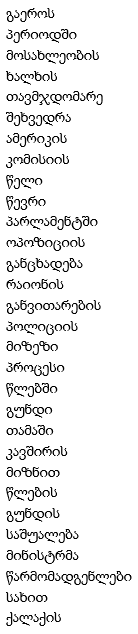
\includegraphics[scale=0.665]{images/wc_ka_list}}\\
		horse		& Norden		& \foreignlanguage{russian}{информации}		& yüzde			& \\
		dinner		& Bevölkerung	& \foreignlanguage{russian}{территории}		& karşılık		& \\
		countries	& Partei			& \foreignlanguage{russian}{рынке}			& Devlet			& \\
		restaurant	& Arten			& \foreignlanguage{russian}{программы}		& sırasında		& \\
		back		& Stunden		& \foreignlanguage{russian}{уровень}			& makine		& \\
		women		& Zahl			& \foreignlanguage{russian}{начала}			& içeriye			& \\
		Percentage	& Mannschaft		& \foreignlanguage{russian}{производства}		& okula			& \\
		moment		& Tochter		& \foreignlanguage{russian}{степени}			& mektup		& \\
		changes		& Provinz		& \foreignlanguage{russian}{период}			& haber			& \\
		minutes		& Laden			& \foreignlanguage{russian}{ходе}				& sahibi			& \\
		members	& Betrieb		& \foreignlanguage{russian}{средства}			& Kuzey			& \\
		security		& Beginn		& \foreignlanguage{russian}{основе}			& cevap			& \\
		reason		& Bedeutung		& \foreignlanguage{russian}{граждан}			& şirketi			& \\
		email		& Süden			& \foreignlanguage{russian}{отношения}		& yüzyılda		& \\
		language	& Wochen		& \foreignlanguage{russian}{движения}		& yüzünden		& \\
		peace		& Westen		& \foreignlanguage{russian}{данным}			& dönemde		& \\
		position		& Ergebnis		& \foreignlanguage{russian}{большинство}		& durumunda	& \\
		girl			& Minuten		& \foreignlanguage{russian}{безопасности}		& yola			& \\
		PivotTable	& Dorf			& \foreignlanguage{russian}{участие}			& öğrenci		& \\
		level		& Länge			& \foreignlanguage{russian}{взгляд}			& çocuğun		& \\
		city			& Vertrag		& \foreignlanguage{russian}{культуры}			& sorun			& \\
		agreement	& Jahrhundert	& \foreignlanguage{russian}{группы}			& oğlum			& \\
		table		& Ortsteil		& \foreignlanguage{russian}{директор}			& seçim			& \\
		front		& Landkreis		& \foreignlanguage{russian}{проект}			& isim			& \\
		control		& Hilfe			& \foreignlanguage{russian}{армии}			& doğum		& \\
		others		& Verein			& \foreignlanguage{russian}{положение}		& ilişki			& \\
		thanks		& Hälfte			& \foreignlanguage{russian}{действия}			& masanın		& \\
		attention		& Verbindung	& \foreignlanguage{russian}{целом}			& gözleri			& \\
		hotel		& Zeitpunkt		& \foreignlanguage{russian}{смысле}			& ayında			& \\
		\hline
	\end{tabularx}}
	\caption[List of the 30 chosen mid-frequency nouns for each language (\caps{WC} task)]
		{List of the 30 chosen mid-frequency nouns for each language (\caps{WC} task). The table entries are sorted by frequencies.}
	\label{tab:wc_words}
\end{table}

\newpage

% Table: Chosen verbs for each language
\begin{table}[h]
	\centering
	\renewcommand{\arraystretch}{0.90}
	\scalebox{0.90}{
	\begin{tabularx}{\textwidth}{| X | X | X | X | X |}
		\hline
		\rowcolor{tud9c!50}
		\textbf{EN}	&
		\textbf{DE} 	&
		\textbf{RU} 	&
		\textbf{TR}	&
		\textbf{KA} 	\\
		\hline\hline
		know 		&	sein			&	\foreignlanguage{russian}{знать}		&	yapmak		&
			\multirow{38}{*}{
\includegraphics[scale=0.72]{images/sv_agree_ka_list}}	\\
		speak		&	tun			&	\foreignlanguage{russian}{жить}		&	gitmek		& 	\\
		think		&	gehen		&	\foreignlanguage{russian}{любитъ}	&	gelmek		& 	\\
		understand	&	machen		&	\foreignlanguage{russian}{работать}	&	almak		& 	\\
		remember	&	wissen		&	\foreignlanguage{russian}{ждать}		&	istemek		& 	\\
		eat			&	leben		&	\foreignlanguage{russian}{говорить}	&	çalışmak		& 	\\
		happen		&	arbeiten		&	\foreignlanguage{russian}{думать}		&	bilmek		& 	\\
		get			&	warten		&	\foreignlanguage{russian}{понимать}	&	konuşmak	& 	\\
		come		&	sprechen		&	\foreignlanguage{russian}{мочь}		&	okumak		& 	\\
		avoid		&	denken		&	\foreignlanguage{russian}{хотеть}		&	sevmek		& 	\\
		pretend		&	verstehen	&	\foreignlanguage{russian}{делать}		&	demek		& 	\\
		mitigate		&	wollen		&	\foreignlanguage{russian}{брать}		&	düşünmek	& 	\\
		pray			&	nehmen		&	\foreignlanguage{russian}{давать}		&	yemek		& 	\\
		forgive		&	geben		&	\foreignlanguage{russian}{помнить}	&	içmek		& 	\\
					&	sagen		&										&	başlamak	& 	\\
					&	fragen		&										&	olmak		& 	\\
					&	trinken		&										&	söylemek	& 	\\
					&	essen		&										&	yatmak		& 	\\
					&	passieren	&										&	oturmak		& 	\\
					&	mögen		&										&	sormak		& 	\\
					&	fliegen		&										&	inanmak		& 	\\
					&	haben		&										&	açıklamak	& 	\\
					&				&										&	açmak		&	\\
					&				&										&	affetmek		&	\\
					&				&										&	almak		&	\\
					&				&										&	anlamak		&	\\
					&				&										&	aramak		&	\\
					&				&										&	ağlamak		&	\\
					&				&										&	abartmak	&	\\
					&				&										&	beğenmek	&	\\
					&				&										&	beklemek	&	\\
					&				&										&	atlamak		&	\\
					&				&										&	atmak		&	\\
					&				&										&	azaltmak		&	\\
					&				&										&	korkmak		&	\\
					&				&										&	koşmak		&	\\
					&				&										&	kullanmak	&	\\	
					& 				&	 									&	önermek		&	\\				
		\hline
	\end{tabularx}}
	\caption[List of the chosen verbs for each language (\caps{SVAgree} task)]
		{List of the chosen verbs for each language (\caps{SVAgree} task).}
	\label{tab:sv_agree_words}
\end{table}

\vfill
\hrule
\textbf{Remarks concerning the tables in appendix \vref{sec:appendix_probing} and \vref{sec:appendix_downstream}:} \\
The following tables list the results on probing tasks and downstream tasks in detail. Next to the test scores, the tables furthermore contain the relative rankings of the embeddings per task. These rankings can be found in the columns labeled with `R'. In order to facilitate a quick overview, the top-three performances were highlighted: A \textcolor{gold}{golden} cell background indicates rank 1, \textcolor{silver}{silver} color rank 2, and finally, a \textcolor{bronze}{bronze} color denotes rank 3. The results were produced without hyper-parameter optimization.

\newpage

% Detailed Probing Task Results
% -----------------------------------------------------------------------------------------------------------------------------------------------------
\section{Detailed Probing Task Results}
\label{sec:appendix_probing}

% Results measured by F1 Score
% -----------------------------------------------------------------------------------------------------------------------------------------------------
\subsection{Results measured by F1 Score}

\begin{table}[H]
	\centering
	\renewcommand{\arraystretch}{1.36}
	\begin{adjustbox}{angle=90}
	\scalebox{0.8}{
	\begin{tabularx}{1.1\textheight}{
		| l ? Y | c | Y | c ? Y | c | Y | c | Y | c | Y | c | Y | c ? Y | c | Y | c |
	}
	\hline
	\multicolumn{19}{| c |}{
		\cellcolor{tud9c}\textcolor{white}{
			\textbf{Language: English (F1)}}} 					\\
	\hline

	\rowcolor{tud9c!85}
	\cellcolor{tud9c!85}										&
	\multicolumn{4}{ c ?}{\textbf{Surface Tasks}} 				& 
		\multicolumn{10}{ c ?}{\textbf{Syntactic Tasks}}		&
		\multicolumn{4}{c |}{\textbf{Semantic Tasks}}			\\

	\cellcolor{tud9c!85}										& 
		\multicolumn{2}{ c |}{
			\cellcolor{tud9c!70}\textbf{\caps{SentLen}}} 		&
		\multicolumn{2}{ c ?}{
			\cellcolor{tud9c!70}\textbf{\caps{WC}}} 			&
		\multicolumn{2}{ c |}{
			\cellcolor{tud9c!70}\textbf{\caps{BiShift}}}			&
		\multicolumn{2}{ c |}{
			\cellcolor{tud9c!70}\textbf{\caps{SVAgree}}} 		&
		\multicolumn{2}{ c |}{
			\cellcolor{tud9c!70}\textbf{\caps{SVDist}}} 			&
		\multicolumn{2}{ c |}{
			\cellcolor{tud9c!70}\textbf{\caps{Voice}}}			&
		\multicolumn{2}{ c ?}{
			\cellcolor{tud9c!70}\textbf{\caps{WO}}}			&
		\multicolumn{2}{ c |}{
			\cellcolor{tud9c!70}\textbf{\caps{EOS}}} 			&
		\multicolumn{2}{ c |}{
			\cellcolor{tud9c!70}\textbf{\caps{SubjNum}}}		\\

	\rowcolor{tud9c!55}
	\multirow{-3}{*}{\cellcolor{tud9c!85}\textbf{Embedding}}	&
		\textbf{F1} & \textbf{R} & \textbf{F1} & \textbf{R} & \textbf{F1} & \textbf{R} &
	   	\textbf{F1} & \textbf{R} & \textbf{F1} & \textbf{R} & \textbf{F1} & \textbf{R} &
	   	\textbf{F1} & \textbf{R} & \textbf{F1} & \textbf{R} & \textbf{F1} & \textbf{R} \\
	\hline\hline
	\multicolumn{19}{| l |}{\cellcolor{tud9c!30}\textbf{Size of the data set}} \\ \hline
	\# instances &
                10,000 	& - &
                10,000 	& - &
                10,000 	& - &
                10,000 	& - &
                10,000 	& - &
                9,999 		& - &
                10,000 	& - &
		   10,000 	& - &
                9,448 		& - \\   
	\hline\hline 
	\multicolumn{19}{| l |}{\cellcolor{tud9c!30}\textbf{Majority class (baseline)}} \\ \hline
	\rowcolor{lightgray!30}
	Majority &
                17.9 & - &
                13.3 & - &
                50.2 & - &
                51.1 & - &
                47.5 & - &
                61.0 & - &
                33.4 & - &
		   21.7 & - &
                75.7 & - \\
	\hline\hline   
	\multicolumn{19}{| l |}{\cellcolor{tud9c!30}\textbf{Random embeddings (baseline)}} \\ \hline
	\rowcolor{lightgray!30}
	BOREP &
                00.438 & 10 &
                00.551 & 18 &
                00.488 & 18 &
                00.737 & 18 &
                00.279 & 10 &
                00.776 & 10 &
                00.188 & 15 &
                00.213 & 10 &
                00.844 & 7 \\
        \hline
	 \rowcolor{lightgray!30}
        Random BiLSTM &
                00.549 & 7 &
                00.462 & 20 &
                00.510 & 6 &
                00.819 & 12 &
                00.323 & 5 &
                \cellcolor{bronze}{00.833} & \cellcolor{bronze}{3} &
                00.598 & 4 &
                \cellcolor{bronze}{00.246} & \cellcolor{bronze}{3} &
                \cellcolor{silver}{00.879} & \cellcolor{silver}{2} \\
	\hline\hline
	\multicolumn{19}{| l |}{\cellcolor{tud9c!30}\textbf{Average embeddings (\textit{FastText})}} \\ \hline
	Vanilla average &
                00.240 & 17 &
                00.581 & 17 &
                00.485 & 20 &
                00.775 & 16 &
                00.265 & 13 &
                00.798 & 7 &
                00.201 & 11 &
                00.150 & 19 &
                00.855 & 5 \\
        \hline
        p-Means &
                00.553 & 5 &
                00.657 & 13 &
                00.491 & 15 &
                00.804 & 14 &
                00.309 & 6 &
                00.807 & 6 &
                00.173 & 19 &
                00.231 & 6 &
                00.850 & 6 \\
        \hline
        SIF &
                00.217 & 19 &
                00.634 & 14 &
                00.471 & 21 &
                00.808 & 13 &
                00.256 & 15 &
                00.756 & 15 &
                00.208 & 10 &
                00.144 & 20 &
                00.835 & 8 \\
        \hline
        GEM &
                00.301 & 13 &
                00.778 & 10 &
                00.496 & 11 &
                00.776 & 15 &
                00.300 & 8 &
                00.718 & 19 &
                00.068 & 22 &
                00.206 & 12 &
                00.797 & 10 \\
        \hline
        hier. pooling &
                00.454 & 9 &
                00.354 & 22 &
                00.501 & 9 &
                00.660 & 21 &
                00.271 & 12 &
                00.779 & 8 &
                00.363 & 8 &
                00.232 & 5 &
                00.817 & 9 \\
	\hline\hline
	\multicolumn{19}{| l |}{\cellcolor{tud9c!30}\textbf{Average embeddings (\textit{word2vec})}} \\ \hline
	Vanilla average &
                00.243 & 16 &
                00.803 & 7 &
                00.497 & 10 &
                00.892 & 6 &
                00.255 & 16 &
                00.760 & 13 &
                00.187 & 16 &
                00.172 & 16 &
                00.659 & 17 \\
        \hline
        p-Means &
                00.503 & 8 &
                00.822 & 5 &
                00.502 & 8 &
                \cellcolor{gold}{00.939} & \cellcolor{gold}{1} &
                00.295 & 9 &
                00.764 & 12 &
                00.183 & 18 &
                00.236 & 4 &
                00.656 & 18 \\
        \hline
        SIF &
                00.215 & 20 &
                00.809 & 6 &
                00.506 & 7 &
                00.889 & 8 &
                00.248 & 18 &
                00.741 & 17 &
                00.191 & 14 &
                00.158 & 18 &
                00.619 & 21 \\
        \hline
        GEM &
                00.256 & 14 &
                00.597 & 16 &
                00.494 & 13 &
                00.710 & 20 &
                00.241 & 22 &
                00.684 & 21 &
                00.111 & 21 &
                00.179 & 15 &
                00.573 & 22 \\
        \hline
        hier. pooling &
                00.355 & 12 &
                00.695 & 12 &
                00.493 & 14 &
                00.841 & 10 &
                00.253 & 17 &
                00.724 & 18 &
                00.233 & 9 &
                00.224 & 8 &
                00.633 & 20 \\
	\hline\hline
	\multicolumn{19}{| l |}{\cellcolor{tud9c!30}\textbf{Average embeddings (\textit{Attract-Repel})}} \\ \hline
	Vanilla average &
                00.183 & 21 &
                00.622 & 15 &
                00.491 & 15 &
                00.890 & 7 &
                00.247 & 19 &
                00.753 & 16 &
                00.198 & 13 &
                00.141 & 21 &
                00.738 & 14 \\
        \hline
        p-Means &
                00.585 & 4 &
                \cellcolor{gold}{00.946} & \cellcolor{gold}{1} &
                00.464 & 22 &
                \cellcolor{silver}{00.936} & \cellcolor{silver}{2} &
                00.279 & 10 &
                00.818 & 4 &
                00.186 & 17 &
                00.210 & 11 &
                00.761 & 11 \\
        \hline
        SIF &
                00.162 & 22 &
                00.737 & 11 &
                00.488 & 18 &
                00.903 & 5 &
                00.243 & 21 &
                00.699 & 20 &
                00.200 & 12 &
                00.130 & 22 &
                00.685 & 16 \\
        \hline
        GEM &
                00.230 & 18 &
                00.803 & 7 &
                00.491 & 15 &
                00.743 & 17 &
                00.259 & 14 &
                00.650 & 22 &
                00.148 & 20 &
                00.167 & 17 &
                00.640 & 19 \\
        \hline
        hier. pooling &
                00.419 & 11 &
                00.406 & 21 &
                00.496 & 11 &
                00.835 & 11 &
                00.245 & 20 &
                00.770 & 11 &
                00.370 & 7 &
                00.193 & 13 &
                00.700 & 15 \\
	\hline\hline
	\multicolumn{19}{| l |}{\cellcolor{tud9c!30}\textbf{Trained embeddings}} \\ \hline
	InferSent &
                \cellcolor{bronze}{00.600} & \cellcolor{bronze}{3} &
                \cellcolor{silver}{00.919} & \cellcolor{silver}{2} &
                00.536 & 4 &
                \cellcolor{bronze}{00.912} & \cellcolor{bronze}{3} &
                \cellcolor{silver}{00.414} & \cellcolor{silver}{2} &
                \cellcolor{silver}{00.868} & \cellcolor{silver}{2} &
                \cellcolor{bronze}{00.760} & \cellcolor{bronze}{3} &
                00.230 & 7 &
                \cellcolor{silver}{00.879} & \cellcolor{silver}{2} \\
        \hline
        Quick-Thought &
                \cellcolor{silver}{00.649} & \cellcolor{silver}{2} &
                \cellcolor{bronze}{00.848} & \cellcolor{bronze}{3} &
                \cellcolor{bronze}{00.544} & \cellcolor{bronze}{3} &
                00.887 & 9 &
                \cellcolor{bronze}{00.410} & \cellcolor{bronze}{3} &
                00.811 & 5 &
                \cellcolor{silver}{00.802} & \cellcolor{silver}{2} &
                00.221 & 9 &
                00.758 & 13 \\
        \hline
        sent2vec &
                00.254 & 15 &
                00.786 & 9 &
                00.534 & 5 &
                00.910 & 4 &
                00.301 & 7 &
                00.779 & 8 &
                00.381 & 6 &
                00.191 & 14 &
                00.759 & 12 \\
        \hline
        BERT &
                00.551 & 6 &
                00.531 & 19 &
                \cellcolor{gold}{00.641} & \cellcolor{gold}{1} &
                00.718 & 19 &
                00.406 & 4 &
                00.760 & 13 &
                00.573 & 5 &
                \cellcolor{silver}{00.282} & \cellcolor{silver}{2} &
                00.858 & 4 \\
        \hline
        LASER &
                \cellcolor{gold}{00.697} & \cellcolor{gold}{1} &
                00.832 & 4 &
                \cellcolor{silver}{00.600} & \cellcolor{silver}{2} &
                00.572 & 22 &
                \cellcolor{gold}{00.521} & \cellcolor{gold}{1} &
                \cellcolor{gold}{00.904} & \cellcolor{gold}{1} &
                \cellcolor{gold}{00.846} & \cellcolor{gold}{1} &
                \cellcolor{gold}{00.319} & \cellcolor{gold}{1} &
                \cellcolor{gold}{00.899} & \cellcolor{gold}{1} \\
	\hline
	\end{tabularx}}
	\end{adjustbox}
	\caption[Probing task results for the English language (F1 scores)]{Probing task results for the English language (F1 scores).}
	\label{tab:results_probing_tasks_en}
\end{table}	
\begin{table}[H]
	\centering
	\renewcommand{\arraystretch}{1.36}
	\begin{adjustbox}{angle=90}
	\scalebox{0.8}{
	\begin{tabularx}{1.2\textheight}{
		| l ? Y | c | Y | c ? Y | c | Y | c | Y | c | Y | c | Y | c ? Y | c | Y | c |
	}
	\hline
	\multicolumn{19}{| c |}{
		\cellcolor{tud9c}\textcolor{white}{
			\textbf{Language: German (F1)}}} 					\\
	\hline

	\rowcolor{tud9c!85}
	\cellcolor{tud9c!85}										&
	\multicolumn{4}{ c ?}{\textbf{Surface Tasks}} 				& 
		\multicolumn{10}{ c ?}{\textbf{Syntactic Tasks}}		&
		\multicolumn{4}{c |}{\textbf{Semantic Tasks}}			\\

	\cellcolor{tud9c!85}										& 
		\multicolumn{2}{ c |}{
			\cellcolor{tud9c!70}\textbf{\caps{SentLen}}} 		&
		\multicolumn{2}{ c ?}{
			\cellcolor{tud9c!70}\textbf{\caps{WC}}} 			&
		\multicolumn{2}{ c |}{
			\cellcolor{tud9c!70}\textbf{\caps{BiShift}}}			&
		\multicolumn{2}{ c |}{
			\cellcolor{tud9c!70}\textbf{\caps{SVAgree}}}		&
		\multicolumn{2}{ c |}{
			\cellcolor{tud9c!70}\textbf{\caps{SVDist}}} 			&
		\multicolumn{2}{ c |}{
			\cellcolor{tud9c!70}\textbf{\caps{Voice}}}			&
		\multicolumn{2}{ c ?}{
			\cellcolor{tud9c!70}\textbf{\caps{WO}}}			&
		\multicolumn{2}{ c |}{
			\cellcolor{tud9c!70}\textbf{\caps{EOS}}} 			&
		\multicolumn{2}{ c |}{
			\cellcolor{tud9c!70}\textbf{\caps{SubjNum}}}		\\

	\rowcolor{tud9c!55}
	\multirow{-3}{*}{\cellcolor{tud9c!85}\textbf{Embedding}}	&
		\textbf{F1} & \textbf{R} & \textbf{F1} & \textbf{R} & \textbf{F1} & \textbf{R} &
		\textbf{F1} & \textbf{R} & \textbf{F1} & \textbf{R} & \textbf{F1} & \textbf{R} &
		\textbf{F1} & \textbf{R} & \textbf{F1} & \textbf{R} & \textbf{F1} & \textbf{R} \\
	\hline\hline
	\multicolumn{19}{| l |}{\cellcolor{tud9c!30}\textbf{Size of the data set}} \\ \hline
	\# instances &
                10,000 	& - &
                10,000 	& - &
                10,000 	& - &
                10,000 	& - &
                10,000 	& - &
                9,999	 	& - &
		   10,000 	& - &
                10,000 	& - &
                9,999	 	& - \\   
	\hline\hline 
	\multicolumn{19}{| l |}{\cellcolor{tud9c!30}\textbf{Majority class (baseline)}} \\ \hline
	\rowcolor{lightgray!30}
	Majority &
                19.9 & - &
                14.8 & - &
                50.2 & - &
                50.7 & - &
                43.6 & - &
                50.0 & - &
                33.4 & - &
		   19.3 & - &
                50.0 & - \\
	\hline\hline   
	\multicolumn{19}{| l |}{\cellcolor{tud9c!30}\textbf{Random embeddings (baseline)}} \\ \hline
	\rowcolor{lightgray!30}
	BOREP &
                00.402 & 10 &
                00.668 & 7 &
                00.482 & 22 &
                \cellcolor{silver}{00.846} & \cellcolor{silver}{2} &
                00.327 & 10 &
                00.790 & 17 &
                00.173 & 22 &
                00.205 & 11 &
                00.858 & 15 \\
        \hline
        \rowcolor{lightgray!30}
        Random BiLSTM &
                00.508 & 4 &
                00.577 & 8 &
                00.490 & 16 &
                \cellcolor{gold}{00.847} & \cellcolor{gold}{1} &
                00.399 & 4 &
                00.864 & 4 &
                \cellcolor{silver}{00.735} & \cellcolor{silver}{2} &
                00.229 & 8 &
                00.895 & 7 \\
	\hline\hline
	\multicolumn{19}{| l |}{\cellcolor{tud9c!30}\textbf{Average embeddings (\textit{FastText})}} \\ \hline
	Vanilla average &
                00.195 & 15 &
                00.695 & 6 &
                00.489 & 18 &
                00.822 & 10 &
                00.318 & 14 &
                00.832 & 12 &
                00.215 & 16 &
                00.172 & 15 &
                \cellcolor{bronze}{00.903} & \cellcolor{bronze}{3} \\
        \hline
        p-Means &
                00.492 & 6 &
                00.745 & 4 &
                00.489 & 18 &
                00.837 & 5 &
                00.336 & 9 &
                00.856 & 7 &
                00.199 & 20 &
                00.232 & 6 &
                00.890 & 9 \\
        \hline
        SIF &
                00.164 & 18 &
                00.737 & 5 &
                00.500 & 10 &
                00.813 & 12 &
                00.293 & 17 &
                00.793 & 15 &
                00.216 & 14 &
                00.153 & 19 &
                00.898 & 5 \\
        \hline
        GEM &
                00.249 & 14 &
                \cellcolor{bronze}{00.816} & \cellcolor{bronze}{3} &
                00.512 & 5 &
                00.830 & 7 &
                00.325 & 11 &
                00.854 & 8 &
                00.222 & 12 &
                00.198 & 12 &
                00.889 & 10 \\
        \hline
        hier. pooling &
                00.433 & 9 &
                00.524 & 10 &
                00.492 & 13 &
                00.794 & 15 &
                00.322 & 13 &
                00.762 & 20 &
                00.451 & 6 &
                00.217 & 9 &
                00.833 & 16 \\
	\hline\hline
	\multicolumn{19}{| l |}{\cellcolor{tud9c!30}\textbf{Average embeddings (\textit{word2vec})}} \\ \hline
	Vanilla average &
                00.170 & 17 &
                00.296 & 13 &
                00.491 & 15 &
                00.826 & 8 &
                00.337 & 8 &
                00.860 & 5 &
                00.226 & 11 &
                00.154 & 18 &
                00.891 & 8 \\
        \hline
        p-Means &
                00.482 & 7 &
                00.255 & 15 &
                00.500 & 10 &
                00.818 & 11 &
                00.325 & 11 &
                00.858 & 6 &
                00.174 & 21 &
                00.231 & 7 &
                00.883 & 11 \\
        \hline
        SIF &
                00.143 & 21 &
                00.284 & 14 &
                00.504 & 7 &
                00.800 & 14 &
                00.312 & 15 &
                00.839 & 10 &
                00.220 & 13 &
                00.141 & 21 &
                00.880 & 13 \\
        \hline
        GEM &
                00.185 & 16 &
                00.157 & 19 &
                00.503 & 8 &
                00.640 & 21 &
                00.254 & 20 &
                00.664 & 22 &
                00.205 & 19 &
                00.162 & 16 &
                00.650 & 22 \\
        \hline
        hier. pooling &
                00.280 & 12 &
                00.242 & 16 &
                00.492 & 13 &
                00.790 & 17 &
                00.311 & 16 &
                00.819 & 13 &
                00.249 & 10 &
                00.192 & 14 &
                00.865 & 14 \\
	\hline\hline
	\multicolumn{19}{| l |}{\cellcolor{tud9c!30}\textbf{Average embeddings (\textit{Attract-Repel})}} \\ \hline
	Vanilla average &
                00.156 & 20 &
                00.154 & 20 &
                00.495 & 12 &
                00.808 & 13 &
                00.261 & 19 &
                00.798 & 14 &
                00.216 & 14 &
                00.149 & 20 &
                00.808 & 18 \\
        \hline
        p-Means &
                00.500 & 5 &
                00.238 & 17 &
                00.487 & 20 &
                00.840 & 4 &
                00.339 & 7 &
                \cellcolor{gold}{00.877} & \cellcolor{gold}{1} &
                00.211 & 17 &
                00.237 & 5 &
                00.828 & 17 \\
        \hline
        SIF &
                00.128 & 22 &
                00.130 & 21 &
                00.486 & 21 &
                00.793 & 16 &
                00.224 & 22 &
                00.764 & 19 &
                00.209 & 18 &
                00.123 & 22 &
                00.791 & 19 \\
        \hline
        GEM &
                00.162 & 19 &
                00.185 & 18 &
                00.502 & 9 &
                00.663 & 20 &
                00.239 & 21 &
                00.744 & 21 &
                00.250 & 9 &
                00.161 & 17 &
                00.741 & 21 \\
        \hline
        hier. pooling &
                00.342 & 11 &
                00.128 & 22 &
                00.490 & 16 &
                00.774 & 18 &
                00.270 & 18 &
                00.781 & 18 &
                00.324 & 8 &
                00.211 & 10 &
                00.759 & 20 \\
	\hline\hline
	\multicolumn{19}{| l |}{\cellcolor{tud9c!30}\textbf{Trained embeddings}} \\ \hline
	InferSent &
                \cellcolor{silver}{00.557} & \cellcolor{silver}{2} &
                00.449 & 11 &
                00.505 & 6 &
                00.834 & 6 &
                00.367 & 6 &
                00.838 & 11 &
                \cellcolor{bronze}{00.713} & \cellcolor{bronze}{3} &
                00.242 & 4 &
                00.882 & 12 \\
        \hline
        Quick-Thought &
                \cellcolor{bronze}{00.520} & \cellcolor{bronze}{3} &
                00.346 & 12 &
                \cellcolor{bronze}{00.575} & \cellcolor{bronze}{3} &
                00.825 & 9 &
                \cellcolor{gold}{00.456} & \cellcolor{gold}{1} &
                \cellcolor{bronze}{00.868} & \cellcolor{bronze}{3} &
                00.490 & 5 &
                \cellcolor{silver}{00.269} & \cellcolor{silver}{2} &
                00.901 & 4 \\
        \hline
        sent2vec &
                00.271 & 13 &
                \cellcolor{gold}{00.968} & \cellcolor{gold}{1} &
                00.521 & 4 &
                \cellcolor{bronze}{00.845} & \cellcolor{bronze}{3} &
                00.370 & 5 &
                \cellcolor{silver}{00.874} & \cellcolor{silver}{2} &
                00.429 & 7 &
                00.197 & 13 &
                \cellcolor{gold}{00.906} & \cellcolor{gold}{1} \\
        \hline
        BERT &
                00.467 & 8 &
                00.577 & 8 &
                \cellcolor{gold}{00.636} & \cellcolor{gold}{1} &
                00.771 & 19 &
                \cellcolor{bronze}{00.404} & \cellcolor{bronze}{3} &
                00.793 & 15 &
                00.584 & 4 &
                \cellcolor{silver}{00.269} & \cellcolor{silver}{2} &
                00.896 & 6 \\
        \hline
        LASER &
                \cellcolor{gold}{00.608} & \cellcolor{gold}{1} &
                \cellcolor{silver}{00.861} & \cellcolor{silver}{2} &
                \cellcolor{silver}{00.606} & \cellcolor{silver}{2} &
                00.639 & 22 &
                \cellcolor{silver}{00.448} & \cellcolor{silver}{2} &
                00.854 & 8 &
                \cellcolor{gold}{00.821} & \cellcolor{gold}{1} &
                \cellcolor{gold}{00.307} & \cellcolor{gold}{1} &
                \cellcolor{silver}{00.905} & \cellcolor{silver}{2} \\
	\hline
	\end{tabularx}}
	\end{adjustbox}
	\caption[Probing task results for the German language (F1 scores)]{Probing task results for the German language (F1 scores).}
	\label{tab:results_probing_tasks_de}
\end{table}	
\begin{table}[H]
	\centering
	\renewcommand{\arraystretch}{1.36}
	\begin{adjustbox}{angle=90}
	\scalebox{0.8}{
	\begin{tabularx}{1.2\textheight}{
		| l ? Y | c | Y | c ? Y | c | Y | c | Y | c | Y | c | Y | c ? Y | c | Y | c |
	}
	\hline
	\multicolumn{19}{| c |}{
		\cellcolor{tud9c}\textcolor{white}{
			\textbf{Language: Russian (F1)}}} 					\\
	\hline

	\rowcolor{tud9c!85}
	\cellcolor{tud9c!85}										&
	\multicolumn{4}{ c ?}{\textbf{Surface Tasks}} 				& 
		\multicolumn{10}{ c ?}{\textbf{Syntactic Tasks}}		&
		\multicolumn{4}{c |}{\textbf{Semantic Tasks}}			\\

	\cellcolor{tud9c!85}										&
	\multicolumn{2}{ c |}{
			\cellcolor{tud9c!70}\textbf{\caps{SentLen}}}		&
		\multicolumn{2}{ c ?}{
			\cellcolor{tud9c!70}\textbf{\caps{WC}}} 			&
		\multicolumn{2}{ c |}{
			\cellcolor{tud9c!70}\textbf{\caps{BiShift}}}			&
		\multicolumn{2}{ c |}{
			\cellcolor{tud9c!70}\textbf{\caps{SVAgree}}} 		&
		\multicolumn{2}{ c |}{
			\cellcolor{tud9c!70}\textbf{\caps{SVDist}}}			&
		\multicolumn{2}{ c |}{
			\cellcolor{tud9c!70}\textbf{\caps{Voice}}}			&
		\multicolumn{2}{ c ?}{
			\cellcolor{tud9c!70}\textbf{\caps{WO}}}			&
		\multicolumn{2}{ c |}{
			\cellcolor{tud9c!70}\textbf{\caps{EOS}}} 			&
		\multicolumn{2}{ c |}{
			\cellcolor{tud9c!70}\textbf{\caps{SubjNum}}}		\\

	\rowcolor{tud9c!55}
	\multirow{-3}{*}{\cellcolor{tud9c!85}\textbf{Embedding}}	&
		\textbf{F1} & \textbf{R} & \textbf{F1} & \textbf{R} & \textbf{F1} & \textbf{R} &
		\textbf{F1} & \textbf{R} & \textbf{F1} & \textbf{R} & \textbf{F1} & \textbf{R} &
		\textbf{F1} & \textbf{R} & \textbf{F1} & \textbf{R} & \textbf{F1} & \textbf{R} \\
	\hline\hline
	\multicolumn{19}{| l |}{\cellcolor{tud9c!30}\textbf{Size of the data set}} \\ \hline
	\# instances &
                10,000 	& - &
                10,000 	& - &
                10,000 	& - &
                10,000 	& - &
                10,000 	& - &
                9,999 		& - &
                10,000 	& - &
                10,000 	& - &
                9,999		& - \\   
	\hline\hline 
	\multicolumn{19}{| l |}{\cellcolor{tud9c!30}\textbf{Majority class (baseline)}} \\ \hline
	\rowcolor{lightgray!30}
	Majority &
                17.4 & - &
                09.7 & - &
                51.3 & - &
                50.1 & - &
                42.3 & - &
                68.0 & - &
		   33.4 & - &
                23.6 & - &
                50.0 & - \\
	\hline\hline   
	\multicolumn{19}{| l |}{\cellcolor{tud9c!30}\textbf{Random embeddings (baseline)}} \\ \hline
	\rowcolor{lightgray!30}
	BOREP &
                00.405 & 10 &
                00.515 & 14 &
                00.492 & 15 &
                00.752 & 13 &
                00.231 & 10 &
                00.882 & 6 &
                00.177 & 19 &
                00.209 & 10 &
                00.863 & 9 \\
        \hline
        \rowcolor{lightgray!30}
        Random BiLSTM &
                00.515 & 6 &
                00.552 & 13 &
                00.514 & 5 &
                00.773 & 5 &
                00.272 & 4 &
                \cellcolor{gold}{00.918} & \cellcolor{gold}{1} &
                \cellcolor{bronze}{00.716} & \cellcolor{bronze}{3} &
                00.231 & 6 &
                \cellcolor{bronze}{00.901} & \cellcolor{bronze}{3} \\
	\hline\hline
	\multicolumn{19}{| l |}{\cellcolor{tud9c!30}\textbf{Average embeddings (\textit{FastText})}} \\ \hline
	Vanilla average &
                00.208 & 15 &
                00.672 & 12 &
                00.483 & 18 &
                00.754 & 10 &
                00.216 & 14 &
                00.883 & 5 &
                00.213 & 14 &
                00.125 & 20 &
                \cellcolor{silver}{00.913} & \cellcolor{silver}{2} \\
        \hline
        p-Means &
                00.519 & 5 &
                00.673 & 11 &
                00.474 & 20 &
                00.771 & 6 &
                00.256 & 7 &
                \cellcolor{silver}{00.912} & \cellcolor{silver}{2} &
                00.202 & 17 &
                00.239 & 4 &
                00.899 & 4 \\
        \hline
        SIF &
                00.193 & 18 &
                00.694 & 10 &
                00.494 & 14 &
                00.754 & 10 &
                00.213 & 17 &
                00.848 & 11 &
                00.212 & 15 &
                00.126 & 19 &
                \cellcolor{gold}{00.916} & \cellcolor{gold}{1} \\
        \hline
        GEM &
                00.257 & 14 &
                00.743 & 9 &
                00.501 & 8 &
                00.745 & 14 &
                00.226 & 11 &
                \cellcolor{bronze}{00.895} & \cellcolor{bronze}{3} &
                00.167 & 20 &
                00.197 & 13 &
                00.876 & 7 \\
        \hline
        hier. pooling &
                00.456 & 8 &
                00.443 & 16 &
                00.499 & 9 &
                00.707 & 15 &
                00.223 & 12 &
                00.856 & 10 &
                00.406 & 6 &
                00.215 & 9 &
                00.851 & 11 \\
	\hline\hline
	\multicolumn{19}{| l |}{\cellcolor{tud9c!30}\textbf{Average embeddings (\textit{word2vec})}} \\ \hline
	Vanilla average &
                00.207 & 16 &
                \cellcolor{bronze}{00.947} & \cellcolor{bronze}{3} &
                00.498 & 10 &
                \cellcolor{bronze}{00.795} & \cellcolor{bronze}{3} &
                00.222 & 13 &
                00.844 & 13 &
                00.208 & 16 &
                00.168 & 14 &
                00.851 & 11 \\
        \hline
        p-Means &
                00.509 & 7 &
                \cellcolor{gold}{00.990} & \cellcolor{gold}{1} &
                00.497 & 11 &
                \cellcolor{silver}{00.800} & \cellcolor{silver}{2} &
                00.240 & 8 &
                00.862 & 9 &
                00.166 & 21 &
                00.226 & 7 &
                00.838 & 15 \\
        \hline
        SIF &
                00.163 & 19 &
                00.937 & 4 &
                00.497 & 11 &
                00.779 & 4 &
                00.214 & 15 &
                00.819 & 15 &
                00.220 & 12 &
                00.147 & 18 &
                00.851 & 11 \\
        \hline
        GEM &
                00.154 & 20 &
                00.803 & 7 &
                00.504 & 7 &
                00.653 & 17 &
                00.214 & 15 &
                00.619 & 17 &
                00.162 & 22 &
                00.151 & 17 &
                00.633 & 19 \\
        \hline
        hier. pooling &
                00.359 & 11 &
                00.854 & 6 &
                00.497 & 11 &
                00.761 & 9 &
                00.235 & 9 &
                00.827 & 14 &
                00.241 & 9 &
                00.208 & 11 &
                00.810 & 16 \\
	\hline\hline
	\multicolumn{19}{| l |}{\cellcolor{tud9c!30}\textbf{Average embeddings (\textit{Attract-Repel})}} \\ \hline
	Vanilla average &
                00.075 & 22 &
                00.295 & 20 &
                00.456 & 22 &
                00.505 & 22 &
                00.195 & 20 &
                00.502 & 21 &
                00.225 & 10 &
                00.083 & 22 &
                00.635 & 17 \\
        \hline
        p-Means &
                00.452 & 9 &
                00.398 & 17 &
                00.481 & 19 &
                00.507 & 21 &
                00.197 & 19 &
                00.619 & 17 &
                00.185 & 18 &
                00.234 & 5 &
                00.631 & 20 \\
        \hline
        SIF &
                00.091 & 21 &
                00.294 & 21 &
                00.469 & 21 &
                00.514 & 19 &
                00.193 & 22 &
                00.490 & 22 &
                00.219 & 13 &
                00.089 & 21 &
                00.634 & 18 \\
        \hline
        GEM &
                00.328 & 12 &
                00.294 & 21 &
                00.488 & 16 &
                00.510 & 20 &
                00.207 & 18 &
                00.585 & 19 &
                00.223 & 11 &
                00.204 & 12 &
                00.615 & 22 \\
        \hline
        hier. pooling &
                00.201 & 17 &
                00.320 & 19 &
                00.488 & 16 &
                00.516 & 18 &
                00.194 & 21 &
                00.557 & 20 &
                00.247 & 8 &
                00.157 & 16 &
                00.628 & 21 \\
	\hline\hline
	\multicolumn{19}{| l |}{\cellcolor{tud9c!30}\textbf{Trained embeddings}} \\ \hline
	InferSent &
                \cellcolor{silver}{00.576} & \cellcolor{silver}{2} &
                00.389 & 18 &
                00.530 & 4 &
                00.753 & 12 &
                00.264 & 6 &
                00.891 & 4 &
                00.651 & 4 &
                00.225 & 8 &
                00.891 & 5 \\
        \hline
        Quick-Thought &
                \cellcolor{bronze}{00.574} & \cellcolor{bronze}{3} &
                00.904 & 5 &
                \cellcolor{bronze}{00.550} & \cellcolor{bronze}{3} &
                00.768 & 8 &
                \cellcolor{bronze}{00.344} & \cellcolor{bronze}{3} &
                00.846 & 12 &
                \cellcolor{silver}{00.727} & \cellcolor{silver}{2} &
                \cellcolor{silver}{00.253} & \cellcolor{silver}{2} &
                00.842 & 14 \\
        \hline
        sent2vec &
                00.273 & 13 &
                \cellcolor{silver}{00.968} & \cellcolor{silver}{2} &
                00.506 & 6 &
                \cellcolor{gold}{00.822} & \cellcolor{gold}{1} &
                00.269 & 5 &
                00.871 & 8 &
                00.351 & 7 &
                00.165 & 15 &
                00.876 & 7 \\
        \hline
        BERT &
                00.540 & 4 &
                00.495 & 15 &
                \cellcolor{gold}{00.597} & \cellcolor{gold}{1} &
                00.673 & 16 &
                \cellcolor{silver}{00.375} & \cellcolor{silver}{2} &
                00.802 & 16 &
                00.585 & 5 &
                \cellcolor{bronze}{00.252} & \cellcolor{bronze}{3} &
                00.852 & 10 \\
        \hline
        LASER &
                \cellcolor{gold}{00.636} & \cellcolor{gold}{1} &
                00.776 & 8 &
                \cellcolor{silver}{00.574} & \cellcolor{silver}{2} &
                00.769 & 7 &
                \cellcolor{gold}{00.496} & \cellcolor{gold}{1} &
                00.877 & 7 &
                \cellcolor{gold}{00.779} & \cellcolor{gold}{1} &
                \cellcolor{gold}{00.294} & \cellcolor{gold}{1} &
                00.878 & 6 \\
	\hline
	\end{tabularx}}
	\end{adjustbox}
	\caption[Probing task results for the Russian language (F1 scores)]{Probing task results for the Russian language (F1 scores).}
	\label{tab:results_probing_tasks_ru}
\end{table}	
\begin{table}[H]
	\centering
	\renewcommand{\arraystretch}{1.36}
	\begin{adjustbox}{angle=90}
	\scalebox{0.8}{
	\begin{tabularx}{1.2\textheight}{
		| l ? Y | c | Y | c ? Y | c | Y | c | Y | c | Y | c | Y | c ? Y | c | Y | c |
	}
	\hline
	\multicolumn{19}{| c |}{
		\cellcolor{tud9c}\textcolor{white}{
			\textbf{Language: Turkish (F1)}}} 					\\
	\hline

	\rowcolor{tud9c!85}
	\cellcolor{tud9c!85}										&
	\multicolumn{4}{ c ?}{\textbf{Surface Tasks}} 				& 
		\multicolumn{10}{ c ?}{\textbf{Syntactic Tasks}}		&
		\multicolumn{4}{c |}{\textbf{Semantic Tasks}}			\\

	\cellcolor{tud9c!85}										&
	\multicolumn{2}{ c |}{
			\cellcolor{tud9c!70}\textbf{\caps{SentLen}}}		&
		\multicolumn{2}{ c ?}{
			\cellcolor{tud9c!70}\textbf{\caps{WC}}} 			&
		\multicolumn{2}{ c |}{
			\cellcolor{tud9c!70}\textbf{\caps{BiShift}}}			&
		\multicolumn{2}{ c |}{
			\cellcolor{tud9c!70}\textbf{\caps{SVAgree}}} 		&
		\multicolumn{2}{ c |}{
			\cellcolor{tud9c!70}\textbf{\caps{SVDist}}} 			&
		\multicolumn{2}{ c |}{
			\cellcolor{tud9c!70}\textbf{\caps{Voice}}}			&
		\multicolumn{2}{ c ?}{
			\cellcolor{tud9c!70}\textbf{\caps{WO}}}			&
		\multicolumn{2}{ c |}{
			\cellcolor{tud9c!70}\textbf{\caps{EOS}}} 			&
		\multicolumn{2}{ c |}{
			\cellcolor{tud9c!70}\textbf{\caps{SubjNum}}}		\\

	\rowcolor{tud9c!55}
	\multirow{-3}{*}{\cellcolor{tud9c!85}\textbf{Embedding}}	&
		\textbf{F1} & \textbf{R} & \textbf{F1} & \textbf{R} & \textbf{F1} & \textbf{R} &
		\textbf{F1} & \textbf{R} & \textbf{F1} & \textbf{R} & \textbf{F1} & \textbf{R} &
		\textbf{F1} & \textbf{R} & \textbf{F1} & \textbf{R} & \textbf{F1} & \textbf{R} \\
	\hline\hline
	\multicolumn{19}{| l |}{\cellcolor{tud9c!30}\textbf{Size of the data set}} \\ \hline
	\# instances &
                10,000 	& - &
                10,000 	& - &
                10,000 	& - &
                10,000 	& - &
                2,750 		& - &
                8,416 		& - &
                10,000 	& - &
                10,000 	& - &
                4,030 		& - \\   
	\hline\hline 
	\multicolumn{19}{| l |}{\cellcolor{tud9c!30}\textbf{Majority class (baseline)}} \\ \hline
	\rowcolor{lightgray!30}
	Majority &
                37.3 & - &
                12.6 & - &
                50.5 & - &
                50.6 & - &
                39.0 & - &
                86.2 & - &
		   33.4 & - &
                23.7 & - &
                83.4 & - \\
	\hline\hline   
	\multicolumn{19}{| l |}{\cellcolor{tud9c!30}\textbf{Random embeddings (baseline)}} \\ \hline
	\rowcolor{lightgray!30}
	BOREP &
                00.407 & 10 &
                00.673 & 18 &
                00.486 & 22 &
                00.599 & 20 &
                00.411 & 11 &
                00.661 & 12 &
                00.162 & 19 &
                00.328 & 12 &
                00.703 & 9 \\
        \hline
        \rowcolor{lightgray!30}
        Random BiLSTM &
                00.514 & 5 &
                00.591 & 19 &
                00.553 & 5 &
                00.712 & 4 &
                00.437 & 6 &
                \cellcolor{bronze}{00.703} & \cellcolor{bronze}{3} &
                \cellcolor{bronze}{00.656} & \cellcolor{bronze}{3} &
                00.382 & 4 &
                00.736 & 7 \\
	\hline\hline
	\multicolumn{19}{| l |}{\cellcolor{tud9c!30}\textbf{Average embeddings (\textit{FastText})}} \\ \hline
	Vanilla average &
                00.174 & 18 &
                00.705 & 16 &
                00.487 & 20 &
                00.631 & 17 &
                00.359 & 15 &
                00.682 & 6 &
                00.203 & 13 &
                00.264 & 18 &
                \cellcolor{bronze}{00.752} & \cellcolor{bronze}{3} \\
        \hline
        p-Means &
                00.511 & 6 &
                00.761 & 13 &
                00.487 & 20 &
                00.642 & 15 &
                00.439 & 5 &
                00.690 & 4 &
                00.161 & 20 &
                00.353 & 9 &
                00.744 & 5 \\
        \hline
        SIF &
                00.158 & 20 &
                00.738 & 14 &
                00.492 & 17 &
                00.643 & 14 &
                00.352 & 16 &
                00.689 & 5 &
                00.203 & 13 &
                00.249 & 20 &
                \cellcolor{bronze}{00.752} & \cellcolor{bronze}{3} \\
        \hline
        GEM &
                00.276 & 13 &
                00.798 & 10 &
                00.503 & 9 &
                00.613 & 19 &
                00.380 & 13 &
                \cellcolor{silver}{00.710} & \cellcolor{silver}{2} &
                00.090 & 22 &
                00.305 & 13 &
                \cellcolor{silver}{00.759} & \cellcolor{silver}{2} \\
        \hline
        hier. pooling &
                00.419 & 9 &
                00.516 & 20 &
                00.507 & 6 &
                00.557 & 22 &
                00.420 & 9 &
                00.627 & 18 &
                00.322 & 7 &
                00.356 & 7 &
                00.697 & 10 \\
	\hline\hline
	\multicolumn{19}{| l |}{\cellcolor{tud9c!30}\textbf{Average embeddings (\textit{word2vec})}} \\ \hline
	Vanilla average &
                00.192 & 17 &
                00.873 & 4 &
                00.496 & 13 &
                00.699 & 7 &
                00.345 & 17 &
                00.659 & 14 &
                00.190 & 15 &
                00.279 & 16 &
                00.621 & 12 \\
        \hline
        p-Means &
                00.471 & 8 &
                \cellcolor{silver}{00.916} & \cellcolor{silver}{2} &
                00.504 & 8 &
                00.695 & 11 &
                00.425 & 8 &
                00.667 & 10 &
                00.166 & 18 &
                00.342 & 10 &
                00.617 & 14 \\
        \hline
        SIF &
                00.170 & 19 &
                00.873 & 4 &
                00.492 & 17 &
                00.699 & 7 &
                00.338 & 18 &
                00.656 & 15 &
                00.211 & 10 &
                00.265 & 17 &
                00.617 & 14 \\
        \hline
        GEM &
                00.202 & 15 &
                00.685 & 17 &
                00.495 & 14 &
                00.593 & 21 &
                00.323 & 19 &
                00.576 & 22 &
                00.105 & 21 &
                00.250 & 19 &
                00.587 & 20 \\
        \hline
        hier. pooling &
                00.358 & 12 &
                00.840 & 7 &
                00.498 & 12 &
                00.640 & 16 &
                00.412 & 10 &
                00.639 & 16 &
                00.290 & 8 &
                00.336 & 11 &
                00.602 & 19 \\
	\hline\hline
	\multicolumn{19}{| l |}{\cellcolor{tud9c!30}\textbf{Average embeddings (\textit{Attract-Repel})}} \\ \hline
	Vanilla average &
                00.139 & 21 &
                00.768 & 12 &
                00.500 & 11 &
                00.699 & 7 &
                00.298 & 22 &
                00.625 & 19 &
                00.212 & 9 &
                00.245 & 22 &
                00.605 & 18 \\
        \hline
        p-Means &
                \cellcolor{bronze}{00.527} & \cellcolor{bronze}{3} &
                \cellcolor{gold}{00.936} & \cellcolor{gold}{1} &
                00.493 & 15 &
                00.699 & 7 &
                00.442 & 4 &
                00.681 & 7 &
                00.172 & 17 &
                00.369 & 5 &
                00.608 & 17 \\
        \hline
        SIF &
                00.127 & 22 &
                00.833 & 8 &
                00.506 & 7 &
                00.710 & 5 &
                00.300 & 21 &
                00.622 & 20 &
                00.205 & 12 &
                00.247 & 21 &
                00.612 & 16 \\
        \hline
        GEM &
                00.196 & 16 &
                00.783 & 11 &
                00.490 & 19 &
                00.629 & 18 &
                00.302 & 20 &
                00.590 & 21 &
                00.188 & 16 &
                00.281 & 15 &
                00.580 & 22 \\
        \hline
        hier. pooling &
                00.395 & 11 &
                00.722 & 15 &
                00.501 & 10 &
                00.645 & 13 &
                00.399 & 12 &
                00.634 & 17 &
                00.360 & 6 &
                00.358 & 6 &
                00.584 & 21 \\
	\hline\hline
	\multicolumn{19}{| l |}{\cellcolor{tud9c!30}\textbf{Trained embeddings}} \\ \hline
	InferSent &
                00.522 & 4 &
                00.447 & 22 &
                00.565 & 4 &
                00.658 & 12 &
                00.432 & 7 &
                00.670 & 9 &
                00.650 & 4 &
                \cellcolor{silver}{00.398} & \cellcolor{silver}{2} &
                00.708 & 8 \\
        \hline
        Quick-Thought &
                00.504 & 7 &
                00.867 & 6 &
                \cellcolor{silver}{00.587} & \cellcolor{silver}{2} &
                \cellcolor{silver}{00.737} & \cellcolor{silver}{2} &
                \cellcolor{bronze}{00.448} & \cellcolor{bronze}{3} &
                00.660 & 13 &
                \cellcolor{gold}{00.768} & \cellcolor{gold}{1} &
                00.356 & 7 &
                00.621 & 12 \\
        \hline
        sent2vec &
                00.237 & 14 &
                \cellcolor{bronze}{00.891} & \cellcolor{bronze}{3} &
                00.493 & 15 &
                00.701 & 6 &
                00.367 & 14 &
                00.663 & 11 &
                00.210 & 11 &
                00.288 & 14 &
                00.663 & 11 \\
        \hline
        BERT &
                \cellcolor{silver}{00.583} & \cellcolor{silver}{2} &
                00.494 & 21 &
                \cellcolor{bronze}{00.585} & \cellcolor{bronze}{3} &
                \cellcolor{bronze}{00.725} & \cellcolor{bronze}{3} &
                \cellcolor{silver}{00.454} & \cellcolor{silver}{2} &
                00.676 & 8 &
                00.585 & 5 &
                \cellcolor{bronze}{00.396} & \cellcolor{bronze}{3} &
                00.744 & 5 \\
        \hline
        LASER &
                \cellcolor{gold}{00.615} & \cellcolor{gold}{1} &
                00.805 & 9 &
                \cellcolor{gold}{00.596} & \cellcolor{gold}{1} &
                \cellcolor{gold}{00.774} & \cellcolor{gold}{1} &
                \cellcolor{gold}{00.536} & \cellcolor{gold}{1} &
                \cellcolor{gold}{00.768} & \cellcolor{gold}{1} &
                \cellcolor{silver}{00.743} & \cellcolor{silver}{2} &
                \cellcolor{gold}{00.472} & \cellcolor{gold}{1} &
                \cellcolor{gold}{00.803} & \cellcolor{gold}{1} \\
	\hline
	\end{tabularx}}
	\end{adjustbox}
	\caption[Probing task results for the Turkish language (F1 scores)]{Probing task results for the Turkish language (F1 scores).}
	\label{tab:results_probing_tasks_tr}
\end{table}	
\begin{table}[H]
	\centering
	\renewcommand{\arraystretch}{1.36}
	\begin{adjustbox}{angle=90}
	\scalebox{0.8}{
	\begin{tabularx}{1.2\textheight}{
		| l ? Y | c | Y | c ? Y | c | Y | c | Y | c | Y | c ? Y | c |
	}
	\hline
	\multicolumn{15}{| c |}{
		\cellcolor{tud9c}\textcolor{white}{
			\textbf{Language: Georgian (F1)}}} 				\\
	\hline

	\rowcolor{tud9c!85}
	\cellcolor{tud9c!85}										&
	\multicolumn{4}{ c ?}{\textbf{Surface Tasks}} 				& 
		\multicolumn{8}{ c ?}{\textbf{Syntactic Tasks}}			&
		\multicolumn{2}{c |}{\textbf{Semantic Tasks}}			\\

	\cellcolor{tud9c!85}										& 
		\multicolumn{2}{ c |}{
			\cellcolor{tud9c!70}\textbf{\caps{SentLen}}}		&
		\multicolumn{2}{ c ?}{
			\cellcolor{tud9c!70}\textbf{\caps{WC}}}			&
		\multicolumn{2}{ c |}{
			\cellcolor{tud9c!70}\textbf{\caps{BiShift}}}			&
		\multicolumn{2}{ c |}{
			\cellcolor{tud9c!70}\textbf{\caps{SVAgree}}}		&
		\multicolumn{2}{ c |}{
			\cellcolor{tud9c!70}\textbf{\caps{Voice}}}			&
		\multicolumn{2}{ c ?}{
			\cellcolor{tud9c!70}\textbf{\caps{WO}}}			&
		\multicolumn{2}{ c |}{
			\cellcolor{tud9c!70}\textbf{\caps{EOS}}} 			\\

	\rowcolor{tud9c!55}
	\multirow{-3}{*}{\cellcolor{tud9c!85}\textbf{Embedding}}	&
		\textbf{F1} & \textbf{R} & \textbf{F1} & \textbf{R} &
		\textbf{F1} & \textbf{R} & \textbf{F1} & \textbf{R} & \textbf{F1} & \textbf{R} &
		\textbf{F1} & \textbf{R} & \textbf{F1} & \textbf{R} \\
	\hline\hline
	\multicolumn{15}{| l |}{\cellcolor{tud9c!30}\textbf{Size of the data set}} \\ \hline
	\# instances &
                9,989 		& - &
                10,000 	& - &
                9,993 		& - &
                10,000 	& - &
                10,000 	& - &
                10,000 	& - &
                10,000 	& - \\   
	\hline\hline 
	\multicolumn{15}{| l |}{\cellcolor{tud9c!30}\textbf{Majority class (baseline)}} \\ \hline
	\rowcolor{lightgray!30}
	Majority &
                28.3 & - &
                13.4 & - &
                51.5 & - &
                50.8 & - &
                65.1 & - &
		   33.5 & - &
                28.2 & - \\
	\hline\hline   
	\multicolumn{15}{| l |}{\cellcolor{tud9c!30}\textbf{Random embeddings (baseline)}} \\ \hline
	\rowcolor{lightgray!30}
	BOREP &
                00.373 & 11 &
                00.519 & 15 &
                00.491 & 10 &
                \cellcolor{silver}{00.655} & \cellcolor{silver}{2} &
                00.769 & 4 &
                00.125 & 21 &
                00.348 & 9 \\
        \hline
	\rowcolor{lightgray!30}
        Random BiLSTM &
                00.487 & 5 &
                00.384 & 19 &
                00.503 & 4 &
                \cellcolor{gold}{00.663} & \cellcolor{gold}{1} &
                \cellcolor{gold}{00.788} & \cellcolor{gold}{1} &
                00.525 & 5 &
                00.368 & 5 \\
	\hline\hline
	\multicolumn{15}{| l |}{\cellcolor{tud9c!30}\textbf{Average embeddings (\textit{FastText})}} \\ \hline
	Vanilla average &
                00.140 & 18 &
                00.466 & 16 &
                00.484 & 17 &
                00.634 & 6 &
                00.724 & 13 &
                00.195 & 17 &
                00.241 & 18 \\
        \hline
        p-Means &
                \cellcolor{bronze}{00.498} & \cellcolor{bronze}{3} &
                00.564 & 13 &
                00.487 & 13 &
                00.639 & 4 &
                \cellcolor{silver}{00.782} & \cellcolor{silver}{2} &
                00.139 & 20 &
                00.366 & 6 \\
        \hline
        SIF &
                00.120 & 20 &
                00.461 & 17 &
                00.485 & 16 &
                00.626 & 8 &
                00.698 & 16 &
                00.198 & 16 &
                00.222 & 20 \\
        \hline
        GEM &
                00.291 & 13 &
                00.704 & 4 &
                00.491 & 10 &
                00.630 & 7 &
                00.755 & 8 &
                00.123 & 22 &
                00.316 & 13 \\
        \hline
        hier. pooling &
                00.397 & 9 &
                00.339 & 20 &
                00.497 & 6 &
                00.624 & 9 &
                00.768 & 5 &
                00.276 & 8 &
                00.344 & 10 \\
	\hline\hline
	\multicolumn{15}{| l |}{\cellcolor{tud9c!30}\textbf{Average embeddings (\textit{word2vec})}} \\ \hline
	Vanilla average &
                00.177 & 17 &
                00.578 & 10 &
                00.492 & 9 &
                00.563 & 20 &
                00.692 & 17 &
                00.252 & 9 &
                00.249 & 16 \\
        \hline
        p-Means &
                00.446 & 8 &
                \cellcolor{gold}{00.861} & \cellcolor{gold}{1} &
                00.489 & 12 &
                00.597 & 11 &
                00.720 & 14 &
                00.167 & 19 &
                00.354 & 8 \\
        \hline
        SIF &
                00.124 & 19 &
                00.577 & 11 &
                00.496 & 7 &
                00.580 & 17 &
                00.672 & 19 &
                00.243 & 10 &
                00.230 & 19 \\
        \hline
        GEM &
                00.185 & 16 &
                00.672 & 8 &
                00.486 & 14 &
                00.575 & 19 &
                00.656 & 21 &
                00.202 & 15 &
                00.247 & 17 \\
        \hline
        hier. pooling &
                00.359 & 12 &
                00.701 & 5 &
                00.484 & 17 &
                00.581 & 16 &
                00.731 & 11 &
                00.363 & 7 &
                00.317 & 12 \\
	\hline\hline
	\multicolumn{15}{| l |}{\cellcolor{tud9c!30}\textbf{Average embeddings (\textit{Attract-Repel})}} \\ \hline
	Vanilla average &
                00.107 & 21 &
                00.541 & 14 &
                00.463 & 22 &
                00.594 & 12 &
                00.677 & 18 &
                00.225 & 11 &
                00.213 & 21 \\
        \hline
        p-Means &
                00.488 & 4 &
                \cellcolor{silver}{00.858} & \cellcolor{silver}{2} &
                00.486 & 14 &
                00.609 & 10 &
                00.755 & 8 &
                00.186 & 18 &
                00.360 & 7 \\
        \hline
        SIF &
                00.097 & 22 &
                00.606 & 9 &
                00.481 & 19 &
                00.594 & 12 &
                00.670 & 20 &
                00.214 & 12 &
                00.194 & 22 \\
        \hline
        GEM &
                00.197 & 15 &
                00.698 & 6 &
                00.494 & 8 &
                00.546 & 22 &
                00.621 & 22 &
                00.210 & 13 &
                00.264 & 15 \\
        \hline
        hier. pooling &
                00.390 & 10 &
                00.566 & 12 &
                00.475 & 20 &
                00.591 & 14 &
                00.744 & 10 &
                00.366 & 6 &
                00.319 & 11 \\
	\hline\hline
	\multicolumn{15}{| l |}{\cellcolor{tud9c!30}\textbf{Trained embeddings}} \\ \hline
	InferSent &
                \cellcolor{silver}{00.537} & \cellcolor{silver}{2} &
                00.262 & 22 &
                00.471 & 21 &
                00.635 & 5 &
                \cellcolor{bronze}{00.771} & \cellcolor{bronze}{3} &
                00.543 & 4 &
                \cellcolor{bronze}{00.393} & \cellcolor{bronze}{3} \\
        \hline
        Quick-Thought &
                00.454 & 7 &
                00.679 & 7 &
                \cellcolor{bronze}{00.528} & \cellcolor{bronze}{3} &
                00.579 & 18 &
                00.707 & 15 &
                \cellcolor{gold}{00.787} & \cellcolor{gold}{1} &
                00.387 & 4 \\
        \hline
        sent2vec &
                00.240 & 14 &
                \cellcolor{bronze}{00.799} & \cellcolor{bronze}{3} &
                00.501 & 5 &
                \cellcolor{bronze}{00.650} & \cellcolor{bronze}{3} &
                00.726 & 12 &
                00.206 & 14 &
                00.294 & 14 \\
        \hline
        BERT &
                00.472 & 6 &
                00.446 & 18 &
                \cellcolor{gold}{00.586} & \cellcolor{gold}{1} &
                00.549 & 21 &
                00.761 & 7 &
                \cellcolor{bronze}{00.584} & \cellcolor{bronze}{3} &
                \cellcolor{silver}{00.413} & \cellcolor{silver}{2} \\
        \hline
        LASER &
                \cellcolor{gold}{00.705} & \cellcolor{gold}{1} &
                00.270 & 21 &
                \cellcolor{silver}{00.533} & \cellcolor{silver}{2} &
                00.590 & 15 &
                00.765 & 6 &
                \cellcolor{silver}{00.640} & \cellcolor{silver}{2} &
                \cellcolor{gold}{00.435} & \cellcolor{gold}{1} \\
	\hline
	\end{tabularx}}
	\end{adjustbox}
	\caption[Probing task results for the Georgian language (F1 scores)]{Probing task results for the Georgian language (F1 scores).}
	\label{tab:results_probing_tasks_ka}
\end{table}	

% Table: Top three counts
\begin{tikzpicture}[scale=1.0,every node/.style={scale=1.0}]
	\begin{axis}[
    		title=\textbf{Top-three scores (EN)},
		scale only axis,
		clip=false,
		separate axis lines,
		xtick={1,2,3,4,5,6,7,8,9,10,11,12},
        	x tick style={draw=none},
        	xticklabels={,,},
		width=4cm,height=1.9cm,
		tick label style={font=\footnotesize},
		xticklabel style={rotate=90},
		ymajorgrids,
    		grid style={line width=.1pt, draw=gray!10},
		ymin=0,ymax=1.0,
		every axis plot/.append style={
          		ybar,
          		bar width=6.0,
          		bar shift=0.5pt,
			fill
		},
		scaled y ticks=false,
		y tick label style={
        		/pgf/number format/.cd,
            		fixed,
            		fixed zerofill,
            		precision=2,
        		/tikz/.cd
    		}
	]

		\addplot[blue] coordinates {(1,0.00)};
     	 	\addplot[blue!80] coordinates {(2,0.33)};
      		\addplot[blue!60] coordinates {(3,0.00)};
      		\addplot[blue!40] coordinates {(4,0.00)};
		\addplot[blue!20] coordinates {(5,0.00)};
     	 	\addplot[gray] coordinates {(6,0.00)};
      		\addplot[lightgray] coordinates {(7,0.33)};
      		\addplot[red] coordinates {(8,0.78)};
     	 	\addplot[red!80] coordinates {(9,0.56)};
      		\addplot[red!60] coordinates {(10,0.00)};
      		\addplot[red!40] coordinates {(11,0.22)};
		\addplot[red!20] coordinates {(12,0.78)};

		\node at (axis cs: 1,0.9) {\footnotesize 0};
		\node at (axis cs: 2,0.9) {\footnotesize 3};
		\node at (axis cs: 3,0.9) {\footnotesize 0};
		\node at (axis cs: 4,0.9) {\footnotesize 0};
		\node at (axis cs: 5,0.9) {\footnotesize 0};
		\node at (axis cs: 6,0.9) {\footnotesize 0};
		\node at (axis cs: 7,0.9) {\footnotesize 3};
		\node at (axis cs: 8,0.9) {\footnotesize 7};
		\node at (axis cs: 9,0.9) {\footnotesize 5};
		\node at (axis cs: 10,0.9) {\footnotesize 0};
		\node at (axis cs: 11,0.9) {\footnotesize 2};
		\node at (axis cs: 12,0.9) {\footnotesize 7};
	\end{axis}
\end{tikzpicture}

\begin{tikzpicture}[scale=1.0,every node/.style={scale=1.0}]
	\begin{axis}[
    		title=\textbf{Top-three scores (DE)},
		scale only axis,
		clip=false,
		separate axis lines,
		xtick={1,2,3,4,5,6,7,8,9,10,11,12},
        	x tick style={draw=none},
        	xticklabels={,,},
		width=4cm,height=1.9cm,
		tick label style={font=\footnotesize},
		xticklabel style={rotate=90},
		ymajorgrids,
    		grid style={line width=.1pt, draw=gray!10},
		ymin=0,ymax=1.0,
		every axis plot/.append style={
          		ybar,
          		bar width=6.0,
          		bar shift=0.5pt,
			fill
		},
		scaled y ticks=false,
		y tick label style={
        		/pgf/number format/.cd,
            		fixed,
            		fixed zerofill,
            		precision=2,
        		/tikz/.cd
    		}
	]

		\addplot[blue] coordinates {(1,0.11)};
     	 	\addplot[blue!80] coordinates {(2,0.11)};
      		\addplot[blue!60] coordinates {(3,0.00)};
      		\addplot[blue!40] coordinates {(4,0.11)};
		\addplot[blue!20] coordinates {(5,0.00)};
     	 	\addplot[gray] coordinates {(6,0.11)};
      		\addplot[lightgray] coordinates {(7,0.22)};
      		\addplot[red] coordinates {(8,0.22)};
     	 	\addplot[red!80] coordinates {(9,0.56)};
      		\addplot[red!60] coordinates {(10,0.44)};
      		\addplot[red!40] coordinates {(11,0.33)};
		\addplot[red!20] coordinates {(12,0.78)};

		\node at (axis cs: 1,0.9) {\footnotesize 1};
		\node at (axis cs: 2,0.9) {\footnotesize 1};
		\node at (axis cs: 3,0.9) {\footnotesize 0};
		\node at (axis cs: 4,0.9) {\footnotesize 1};
		\node at (axis cs: 5,0.9) {\footnotesize 0};
		\node at (axis cs: 6,0.9) {\footnotesize 1};
		\node at (axis cs: 7,0.9) {\footnotesize 2};
		\node at (axis cs: 8,0.9) {\footnotesize 2};
		\node at (axis cs: 9,0.9) {\footnotesize 5};
		\node at (axis cs: 10,0.9) {\footnotesize 4};
		\node at (axis cs: 11,0.9) {\footnotesize 3};
		\node at (axis cs: 12,0.9) {\footnotesize 7};
	\end{axis}
\end{tikzpicture}

\begin{tikzpicture}[scale=1.0,every node/.style={scale=1.0}]
	\begin{axis}[
    		title=\textbf{Top-three scores (RU)},
		scale only axis,
		clip=false,
		separate axis lines,
		xtick={1,2,3,4,5,6,7,8,9,10,11,12},
        	x tick style={draw=none},
        	xticklabels={,,},
		width=4cm,height=1.9cm,
		tick label style={font=\footnotesize},
		xticklabel style={rotate=90},
		ymajorgrids,
    		grid style={line width=.1pt, draw=gray!10},
		ymin=0,ymax=1.0,
		every axis plot/.append style={
          		ybar,
          		bar width=6.0,
          		bar shift=0.5pt,
			fill
		},
		scaled y ticks=false,
		y tick label style={
        		/pgf/number format/.cd,
            		fixed,
            		fixed zerofill,
            		precision=2,
        		/tikz/.cd
    		}
	]

		\addplot[blue] coordinates {(1,0.33)};
     	 	\addplot[blue!80] coordinates {(2,0.33)};
      		\addplot[blue!60] coordinates {(3,0.11)};
      		\addplot[blue!40] coordinates {(4,0.11)};
		\addplot[blue!20] coordinates {(5,0.00)};
     	 	\addplot[gray] coordinates {(6,0.00)};
      		\addplot[lightgray] coordinates {(7,0.33)};
      		\addplot[red] coordinates {(8,0.11)};
     	 	\addplot[red!80] coordinates {(9,0.56)};
      		\addplot[red!60] coordinates {(10,0.22)};
      		\addplot[red!40] coordinates {(11,0.33)};
		\addplot[red!20] coordinates {(12,0.56)};

		\node at (axis cs: 1,0.9) {\footnotesize 3};
		\node at (axis cs: 2,0.9) {\footnotesize 3};
		\node at (axis cs: 3,0.9) {\footnotesize 1};
		\node at (axis cs: 4,0.9) {\footnotesize 1};
		\node at (axis cs: 5,0.9) {\footnotesize 0};
		\node at (axis cs: 6,0.9) {\footnotesize 0};
		\node at (axis cs: 7,0.9) {\footnotesize 3};
		\node at (axis cs: 8,0.9) {\footnotesize 1};
		\node at (axis cs: 9,0.9) {\footnotesize 5};
		\node at (axis cs: 10,0.9) {\footnotesize 2};
		\node at (axis cs: 11,0.9) {\footnotesize 3};
		\node at (axis cs: 12,0.9) {\footnotesize 5};
	\end{axis}
\end{tikzpicture}

\begin{tikzpicture}[scale=1.0,every node/.style={scale=1.0}]
	\begin{axis}[
    		title=\textbf{Top-three scores (TR)},
		scale only axis,
		clip=false,
		separate axis lines,
		xtick={1,2,3,4,5,6,7,8,9,10,11,12},
        	x tick style={draw=none},
        	xticklabels={,,},
		width=4cm,height=1.9cm,
		tick label style={font=\footnotesize},
		xticklabel style={rotate=90},
		ymajorgrids,
    		grid style={line width=.1pt, draw=gray!10},
		ymin=0,ymax=1.0,
		every axis plot/.append style={
          		ybar,
          		bar width=6.0,
          		bar shift=0.5pt,
			fill
		},
		scaled y ticks=false,
		y tick label style={
        		/pgf/number format/.cd,
            		fixed,
            		fixed zerofill,
            		precision=2,
        		/tikz/.cd
    		}
	]

		\addplot[blue] coordinates {(1,0.11)};
     	 	\addplot[blue!80] coordinates {(2,0.33)};
      		\addplot[blue!60] coordinates {(3,0.11)};
      		\addplot[blue!40] coordinates {(4,0.22)};
		\addplot[blue!20] coordinates {(5,0.00)};
     	 	\addplot[gray] coordinates {(6,0.00)};
      		\addplot[lightgray] coordinates {(7,0.22)};
      		\addplot[red] coordinates {(8,0.11)};
     	 	\addplot[red!80] coordinates {(9,0.44)};
      		\addplot[red!60] coordinates {(10,0.11)};
      		\addplot[red!40] coordinates {(11,0.56)};
		\addplot[red!20] coordinates {(12,0.89)};
		
		\node at (axis cs: 1,0.9) {\footnotesize 1};
		\node at (axis cs: 2,0.9) {\footnotesize 3};
		\node at (axis cs: 3,0.9) {\footnotesize 1};
		\node at (axis cs: 4,0.9) {\footnotesize 2};
		\node at (axis cs: 5,0.9) {\footnotesize 0};
		\node at (axis cs: 6,0.9) {\footnotesize 0};
		\node at (axis cs: 7,0.9) {\footnotesize 2};
		\node at (axis cs: 8,0.9) {\footnotesize 1};
		\node at (axis cs: 9,0.9) {\footnotesize 4};
		\node at (axis cs: 10,0.9) {\footnotesize 1};
		\node at (axis cs: 11,0.9) {\footnotesize 5};
		\node at (axis cs: 12,0.9) {\footnotesize 8};
	\end{axis}
\end{tikzpicture}

\begin{tikzpicture}[scale=1.0,every node/.style={scale=1.0}]
	\begin{axis}[
    		title=\textbf{Top-three scores (KA)},
		scale only axis,
		clip=false,
		separate axis lines,
		xtick={1,2,3,4,5,6,7,8,9,10,11,12},
        	x tick style={draw=none},
        	xticklabels={Average,p-Means,SIF,GEM,Hier. pooling,BOREP,rand. BiLSTM,InferSent,Quick-Th.,sent2vec,BERT,LASER},
		width=4cm,height=1.9cm,
		tick label style={font=\footnotesize},
		xticklabel style={rotate=90},
		ymajorgrids,
    		grid style={line width=.1pt, draw=gray!10},
		ymin=0,ymax=1.0,
		every axis plot/.append style={
          		ybar,
          		bar width=6.0,
          		bar shift=0.5pt,
			fill
		},
		scaled y ticks=false,
		y tick label style={
        		/pgf/number format/.cd,
            		fixed,
            		fixed zerofill,
            		precision=2,
        		/tikz/.cd
    		}
	]

		\addplot[blue] coordinates {(1,0.00)};
     	 	\addplot[blue!80] coordinates {(2,0.57)};
      		\addplot[blue!60] coordinates {(3,0.00)};
      		\addplot[blue!40] coordinates {(4,0.00)};
		\addplot[blue!20] coordinates {(5,0.00)};
     	 	\addplot[gray] coordinates {(6,0.14)};
      		\addplot[lightgray] coordinates {(7,0.29)};
      		\addplot[red] coordinates {(8,0.43)};
     	 	\addplot[red!80] coordinates {(9,0.29)};
      		\addplot[red!60] coordinates {(10,0.29)};
      		\addplot[red!40] coordinates {(11,0.43)};
		\addplot[red!20] coordinates {(12,0.57)};

		\node at (axis cs: 1,0.9) {\footnotesize 0};
		\node at (axis cs: 2,0.9) {\footnotesize 4};
		\node at (axis cs: 3,0.9) {\footnotesize 0};
		\node at (axis cs: 4,0.9) {\footnotesize 0};
		\node at (axis cs: 5,0.9) {\footnotesize 0};
		\node at (axis cs: 6,0.9) {\footnotesize 1};
		\node at (axis cs: 7,0.9) {\footnotesize 2};
		\node at (axis cs: 8,0.9) {\footnotesize 3};
		\node at (axis cs: 9,0.9) {\footnotesize 2};
		\node at (axis cs: 10,0.9) {\footnotesize 2};
		\node at (axis cs: 11,0.9) {\footnotesize 3};
		\node at (axis cs: 12,0.9) {\footnotesize 4};
	\end{axis}
\end{tikzpicture}


% Results measured by Accuracy
% -----------------------------------------------------------------------------------------------------------------------------------------------------
\subsection{Results measured by Accuracy}

\begin{table}[H]
	\centering
	\renewcommand{\arraystretch}{2.1}
	\begin{adjustbox}{angle=90}
	\scalebox{0.8}{
	\begin{tabularx}{1.125\textheight}{
		| l ? Y | c | Y | c ? Y | c | Y | c | Y | c | Y | c | Y | c ? Y | c | Y | c |
	}
	\hline
	\multicolumn{19}{| c |}{
		\cellcolor{tud9c}\textcolor{white}{
			\textbf{Language: English (Accuracy)}}} 			\\
	\hline

	\rowcolor{tud9c!85}
	\cellcolor{tud9c!85}										&
	\multicolumn{4}{ c ?}{\textbf{Surface Tasks}} 				& 
		\multicolumn{10}{ c ?}{\textbf{Syntactic Tasks}}		&
		\multicolumn{4}{c |}{\textbf{Semantic Tasks}}			\\

	\cellcolor{tud9c!85}										& 
		\multicolumn{2}{ c |}{
			\cellcolor{tud9c!70}\textbf{\caps{SentLen}}} 		&
		\multicolumn{2}{ c ?}{
			\cellcolor{tud9c!70}\textbf{\caps{WC}}} 			&
		\multicolumn{2}{ c |}{
			\cellcolor{tud9c!70}\textbf{\caps{BiShift}}}			&
		\multicolumn{2}{ c |}{
			\cellcolor{tud9c!70}\textbf{\caps{SVAgree}}} 		&
		\multicolumn{2}{ c |}{
			\cellcolor{tud9c!70}\textbf{\caps{SVDist}}} 			&
		\multicolumn{2}{ c |}{
			\cellcolor{tud9c!70}\textbf{\caps{Voice}}}			&
		\multicolumn{2}{ c ?}{
			\cellcolor{tud9c!70}\textbf{\caps{WO}}}			&
		\multicolumn{2}{ c |}{
			\cellcolor{tud9c!70}\textbf{\caps{EOS}}} 			&
		\multicolumn{2}{ c |}{
			\cellcolor{tud9c!70}\textbf{\caps{SubjNum}}}		\\

	\rowcolor{tud9c!55}
	\multirow{-3}{*}{\cellcolor{tud9c!85}\textbf{Embedding}}	&
		\textbf{F1} & \textbf{R} & \textbf{F1} & \textbf{R} & \textbf{F1} & \textbf{R} &
	   	\textbf{F1} & \textbf{R} & \textbf{F1} & \textbf{R} & \textbf{F1} & \textbf{R} &
	   	\textbf{F1} & \textbf{R} & \textbf{F1} & \textbf{R} & \textbf{F1} & \textbf{R} \\
	\hline\hline
	\multicolumn{19}{| l |}{\cellcolor{tud9c!30}\textbf{Size of the data set}} \\ \hline
	\# instances &
                10,000 	& - &
                10,000 	& - &
                10,000 	& - &
                10,000 	& - &
                10,000 	& - &
                9,999 		& - &
                10,000 	& - &
		   10,000 	& - &
                9,448 		& - \\    
	\hline\hline 
	\multicolumn{19}{| l |}{\cellcolor{tud9c!30}\textbf{Majority class (baseline)}} \\ \hline
	\rowcolor{lightgray!30}
	Majority &
                17.9 & - &
                13.3 & - &
                50.2 & - &
                51.1 & - &
                47.5 & - &
                61.0 & - &
                33.4 & - &
		   21.7 & - &
                75.7 & - \\
	\hline\hline   
	\multicolumn{19}{| l |}{\cellcolor{tud9c!30}\textbf{Random embeddings (baseline)}} \\ \hline
	\rowcolor{lightgray!30}
	BOREP &
                50.728 & 8 &
                65.800 & 10 &
                49.780 & 8 &
                79.680 & 7 &
                58.659 & 11 &
                79.490 & 7 &
                29.591 & 8 &
                27.780 & 6 &
                88.073 & 8 \\
        \hline
	  \rowcolor{lightgray!30}
        Random BiLSTM &
                62.730 & 4 &
                65.999 & 9 &
                51.880 & 6 &
                80.740 & 4 &
                66.110 & 4 &
                \cellcolor{bronze}{83.990} & \cellcolor{bronze}{3} &
                59.889 & 4 &
                \cellcolor{bronze}{31.101} & \cellcolor{bronze}{3} &
                \cellcolor{bronze}{91.174} & \cellcolor{bronze}{3} \\
	\hline\hline
	\multicolumn{19}{| l |}{\cellcolor{tud9c!30}\textbf{Average embeddings (\textit{FastText})}} \\ \hline
	Vanilla average &
                30.220 & 11 &
                75.919 & 8 &
                49.760 & 9 &
                77.430 & 9 &
                61.680 & 7 &
                80.820 & 6 &
                25.811 & 9 &
                24.510 & 10 &
                89.703 & 6 \\
        \hline
        p-Means &
                61.430 & 5 &
                76.119 & 7 &
                49.260 & 12 &
                79.820 & 6 &
                61.050 & 8 &
                82.140 & 4 &
                20.381 & 11 &
                28.880 & 5 &
                89.925 & 4 \\
        \hline
        SIF &
                28.061 & 12 &
                77.518 & 6 &
                49.430 & 11 &
                80.650 & 5 &
                60.810 & 9 &
                77.540 & 10 &
                24.890 & 10 &
                23.350 & 11 &
                88.380 & 7 \\
        \hline
        GEM &
                35.099 & 9 &
                82.572 & 4 &
                49.760 & 9 &
                78.510 & 8 &
                54.700 & 12 &
                73.550 & 12 &
                07.080 & 12 &
                25.770 & 7 &
                85.956 & 10 \\
        \hline
        hier. pooling &
                55.801 & 7 &
                55.287 & 12 &
                50.700 & 7 &
                65.890 & 11 &
                62.810 & 6 &
                78.980 & 9 &
                37.451 & 7 &
                30.080 & 4 &
                87.089 & 9 \\
	\hline\hline
	\multicolumn{19}{| l |}{\cellcolor{tud9c!30}\textbf{Trained embeddings}} \\ \hline
	InferSent &
                \cellcolor{bronze}{68.951} & \cellcolor{bronze}{3} &
                \cellcolor{gold}{94.780} & \cellcolor{gold}{1} &
                54.390 & 4 &
                \cellcolor{gold}{91.320} & \cellcolor{gold}{1} &
                \cellcolor{silver}{69.599} & \cellcolor{silver}{2} &
                \cellcolor{silver}{87.450} & \cellcolor{silver}{2} &
                \cellcolor{bronze}{76.050} & \cellcolor{bronze}{3} &
                25.050 & 8 &
                \cellcolor{silver}{91.311} & \cellcolor{silver}{2} \\
        \hline
        Quick-Thought &
                \cellcolor{silver}{68.970} & \cellcolor{silver}{2} &
                \cellcolor{bronze}{84.480} & \cellcolor{bronze}{3} &
                \cellcolor{bronze}{54.660} & \cellcolor{bronze}{3} &
                \cellcolor{bronze}{88.520} & \cellcolor{bronze}{3} &
                \cellcolor{bronze}{67.321} & \cellcolor{bronze}{3} &
                82.140 & 4 &
                \cellcolor{silver}{80.420} & \cellcolor{silver}{2} &
                24.959 & 9 &
                82.559 & 12 \\
        \hline
        sent2vec &
                31.000 & 10 &
                81.555 & 5 &
                53.190 & 5 &
                \cellcolor{silver}{90.900} & \cellcolor{silver}{2} &
                59.170 & 10 &
                79.090 & 8 &
                38.090 & 6 &
                22.640 & 12 &
                82.845 & 11 \\
        \hline
        BERT &
                59.169 & 6 &
                61.608 & 11 &
                \cellcolor{gold}{64.250} & \cellcolor{gold}{1} &
                72.260 & 10 &
                66.070 & 5 &
                77.360 & 11 &
                56.869 & 5 &
                \cellcolor{silver}{31.921} & \cellcolor{silver}{2} &
                89.713 & 5 \\
        \hline
        LASER &
                \cellcolor{gold}{74.971} & \cellcolor{gold}{1} &
                \cellcolor{silver}{89.979} & \cellcolor{silver}{2} &
                \cellcolor{silver}{59.950} & \cellcolor{silver}{2} &
                57.120 & 12 &
                \cellcolor{gold}{72.921} & \cellcolor{gold}{1} &
                \cellcolor{gold}{90.920} & \cellcolor{gold}{1} &
                \cellcolor{gold}{84.790} & \cellcolor{gold}{1} &
                \cellcolor{gold}{37.790} & \cellcolor{gold}{1} &
                \cellcolor{gold}{92.909} & \cellcolor{gold}{1} \\
	\hline
	\end{tabularx}}
	\end{adjustbox}
	\caption[Probing task results for the English language (accuracy)]{Probing task results for the English language (accuracy).}
	\label{tab:results_probing_tasks_en_acc}
\end{table}	


% Detailed Downstream Task Results
% -----------------------------------------------------------------------------------------------------------------------------------------------------
\section{Detailed Downstream Task Results}
\label{sec:appendix_downstream}

% Results measured by F1 Score
% -----------------------------------------------------------------------------------------------------------------------------------------------------
\subsection{Results measured by F1 Score}

\begin{table}[H]
	\centering
	\renewcommand{\arraystretch}{1.5}
	\begin{adjustbox}{angle=90}
	\scalebox{0.72}{
	\begin{tabular}{
		| l ? >{\centering}m{2.4cm} | c ? >{\centering}m{2.4cm} | c ? >{\centering}m{2.4cm} | c |
	}
	\hline
	\multicolumn{7}{| c |}{
		\cellcolor{tud9c}\textcolor{white}{
			\textbf{Language: English (F1)}}}					\\
	\hline

	\cellcolor{tud9c!85}										& 
		\multicolumn{2}{ c ?}{
			\cellcolor{tud9c!70}\textbf{\caps{ArgMin}}}			&
		\multicolumn{2}{ c ?}{
			\cellcolor{tud9c!70}\textbf{\caps{Senti}}}			&
		\multicolumn{2}{ c |}{
			\cellcolor{tud9c!70}\textbf{\caps{TREC}}}			\\

	\rowcolor{tud9c!55}
	\multirow{-3}{*}{\cellcolor{tud9c!85}\textbf{Embedding}}	&
		\textbf{F1} & \textbf{R} & \textbf{F1} & \textbf{R} & \textbf{F1} & \textbf{R} \\
	\hline\hline
	\multicolumn{7}{| l |}{\cellcolor{tud9c!30}\textbf{Size of the data set}} \\ \hline
	\# instances &
                25,303 	& - &
                14,148 	& - &
                5,952 		& - \\
	\hline\hline 
	\multicolumn{7}{| l |}{\cellcolor{tud9c!30}\textbf{Majority class (baseline)}} \\ \hline
	\rowcolor{lightgray!30}
	Majority &
                56.4 & - &
                64.0 & - &
                22.6 & - \\
	\hline\hline   
	\multicolumn{7}{| l |}{\cellcolor{tud9c!30}\textbf{Random embeddings (baseline)}} \\ \hline
	\rowcolor{lightgray!30}
	BOREP &
                00.542 & 13 &
                00.646 & 9 &
                00.819 & 5 \\
        \hline
	 \rowcolor{lightgray!30}
        Random BiLSTM &
                00.536 & 15 &
                00.688 & 6 &
                00.774 & 9 \\
	\hline\hline
	\multicolumn{7}{| l |}{\cellcolor{tud9c!30}\textbf{Average embeddings (\textit{FastText})}} \\ \hline
	Vanilla average &
                00.550 & 12 &
                00.698 & 4 &
                00.795 & 7 \\
        \hline
        p-Means &
                00.568 & 7 &
                00.695 & 5 &
                00.767 & 10 \\
        \hline
        SIF &
                00.533 & 16 &
                \cellcolor{silver}{00.702} & \cellcolor{silver}{2} &
                00.715 & 13 \\
        \hline
        GEM &
                00.540 & 14 &
                00.646 & 9 &
                00.820 & 4 \\
        \hline
        hier. pooling &
                00.513 & 17 &
                00.627 & 16 &
                00.724 & 12 \\
	\hline\hline
	\multicolumn{7}{| l |}{\cellcolor{tud9c!30}\textbf{Average embeddings (\textit{word2vec})}} \\ \hline
	Vanilla average &
                00.585 & 4 &
                00.639 & 12 &
                00.693 & 16 \\
        \hline
        p-Means &
                00.561 & 9 &
                00.622 & 18 &
                00.713 & 14 \\
        \hline
        SIF &
                00.581 & 5 &
                00.627 & 16 &
                00.644 & 18 \\
        \hline
        GEM &
                00.426 & 22 &
                00.516 & 22 &
                00.576 & 20 \\
        \hline
        hier. pooling &
                00.555 & 11 &
                00.603 & 19 &
                00.697 & 15 \\
	\hline\hline
	\multicolumn{7}{| l |}{\cellcolor{tud9c!30}\textbf{Average embeddings (\textit{Attract-Repel})}} \\ \hline
	Vanilla average &
                00.511 & 18&
                00.630 & 15 &
                00.651 & 17 \\
        \hline
        p-Means &
                00.568 & 7 &
                00.660 & 7 &
                00.748 & 11 \\
        \hline
        SIF &
                00.497 & 19 &
                00.631 & 14 &
                00.554 & 22 \\
        \hline
        GEM &
                00.487 & 21 &
                00.565 & 21 &
                00.564 & 21 \\
        \hline
        hier. pooling &
                00.492 & 20 &
                00.594 & 20 &
                00.641 & 19 \\
	\hline\hline
	\multicolumn{7}{| l |}{\cellcolor{tud9c!30}\textbf{Trained embeddings}} \\ \hline
	InferSent &
                \cellcolor{silver}{00.604} & \cellcolor{silver}{2} &
                \cellcolor{silver}{00.702} & \cellcolor{silver}{2} &
                \cellcolor{gold}{00.920} & \cellcolor{gold}{1} \\
        \hline
        Quick-Thought &
                00.581 & 5 &
                00.636 & 13 &
                00.814 & 6 \\
        \hline
        sent2vec &
                \cellcolor{gold}{00.608} & \cellcolor{gold}{1} &
                00.656 & 8 &
                00.792 & 8 \\
        \hline
        BERT &
                00.558 & 10 &
                00.644 & 11 &
                \cellcolor{silver}{00.876} & \cellcolor{silver}{2} \\
        \hline
        LASER &
                \cellcolor{bronze}{00.596} & \cellcolor{bronze}{3} &
                \cellcolor{gold}{00.727} & \cellcolor{gold}{1} &
                \cellcolor{bronze}{00.851} & \cellcolor{bronze}{3} \\
	\hline
	\end{tabular}}
	\end{adjustbox}
	\caption[Downstream task results for the English language (F1 scores)]{Downstream task results for the English language (F1 scores).}
	\label{tab:downstream_probing_tasks_en}
\end{table}	
\begin{table}[H]
	\centering
	\renewcommand{\arraystretch}{1.5}
	\begin{adjustbox}{angle=90}
	\scalebox{0.72}{
	\begin{tabular}{
		| l ? >{\centering}m{2.4cm} | c ? >{\centering}m{2.4cm} | c ? >{\centering}m{2.4cm} | c |
	}
	\hline
	\multicolumn{7}{| c |}{
		\cellcolor{tud9c}\textcolor{white}{
			\textbf{Language: German (F1)}}} 					\\
	\hline

	\cellcolor{tud9c!85}										& 
		\multicolumn{2}{ c ?}{
			\cellcolor{tud9c!70}\textbf{\caps{ArgMin}}} 		&
		\multicolumn{2}{ c ?}{
			\cellcolor{tud9c!70}\textbf{\caps{Senti}}}			&
		\multicolumn{2}{ c |}{
			\cellcolor{tud9c!70}\textbf{\caps{TREC}}}			\\

	\rowcolor{tud9c!55}
	\multirow{-3}{*}{\cellcolor{tud9c!85}\textbf{Embedding}}	&
		\textbf{F1} & \textbf{R} & \textbf{F1} & \textbf{R} & \textbf{F1} & \textbf{R} \\
	\hline\hline
	\multicolumn{7}{| l |}{\cellcolor{tud9c!30}\textbf{Size of the data set}} \\ \hline
	\# instances &
                25,303 	& - &
                17,908 	& - &
                5,952 	& - \\
	\hline\hline 
	\multicolumn{7}{| l |}{\cellcolor{tud9c!30}\textbf{Majority class (baseline)}} \\ \hline
	\rowcolor{lightgray!30}
	Majority &
                56.4 & - &
                67.8 & - &
                22.6 & - \\
	\hline\hline   
	\multicolumn{7}{| l |}{\cellcolor{tud9c!30}\textbf{Random embeddings (baseline)}} \\ \hline
	\rowcolor{lightgray!30}
	BOREP &
                00.507 & 7 &
                00.545 & 8 &
                00.764 & 4 \\
        \hline
	\rowcolor{lightgray!30}
        Random BiLSTM &
                00.507 & 7 &
                00.559 & 4 &
                00.676 & 9 \\
	\hline\hline
	\multicolumn{7}{| l |}{\cellcolor{tud9c!30}\textbf{Average embeddings (\textit{FastText})}} \\ \hline
	Vanilla average &
                00.507 & 7 &
                00.544 & 9 &
                00.694 & 8 \\
        \hline
        p-Means &
                \cellcolor{silver}{00.534} & \cellcolor{silver}{2} &
                00.550 & 6 &
                \cellcolor{bronze}{00.765} & \cellcolor{bronze}{3} \\
        \hline
        SIF &
                00.514 & 6 &
                00.555 & 5 &
                00.734 & 6 \\
        \hline
        GEM &
                00.521 & 4 &
                \cellcolor{bronze}{00.572} & \cellcolor{bronze}{3} &
                00.730 & 7 \\
        \hline
        hier. pooling &
                00.467 & 16 &
                00.489 & 18 &
                00.601 & 12 \\
	\hline\hline
	\multicolumn{7}{| l |}{\cellcolor{tud9c!30}\textbf{Average embeddings (\textit{word2vec})}} \\ \hline
	Vanilla average &
                00.501 & 11 &
                00.532 & 11 &
                00.581 & 14 \\
        \hline
        p-Means &
                00.479 & 14 &
                00.540 & 10 &
                00.596 & 13 \\
        \hline
        SIF &
                00.499 & 12 &
                00.515 & 14 &
                00.558 & 17 \\
        \hline
        GEM &
                00.391 & 22 &
                00.478 & 19 &
                00.553 & 18 \\
        \hline
        hier. pooling &
                00.471 & 15 &
                00.520 & 13 &
                00.569 & 16 \\
	\hline\hline
	\multicolumn{7}{| l |}{\cellcolor{tud9c!30}\textbf{Average embeddings (\textit{Attract-Repel})}} \\ \hline
	Vanilla average &
                00.432 & 20 &
                00.466 & 20 &
                00.488 & 21 \\
        \hline
        p-Means &
                00.505 & 10 &
                00.529 & 12 &
                00.607 & 11 \\
        \hline
        SIF &
                00.423 & 21 &
                00.461 & 21 &
                00.489 & 20 \\
        \hline
        GEM &
                00.443 & 18 &
                00.506 & 17 &
                00.491 & 19 \\
        \hline
        hier. pooling &
                00.434 & 19 &
                00.432 & 22 &
                00.408 & 22 \\

	\hline\hline
	\multicolumn{7}{| l |}{\cellcolor{tud9c!30}\textbf{Trained embeddings}} \\ \hline
	InferSent &
                00.456 & 17 &
                00.547 & 7 &
                00.580 & 15 \\
        \hline
        Quick-Thought &
                00.497 & 13 &
                00.511 & 16 &
                00.667 & 10 \\
        \hline
        sent2vec &
                \cellcolor{silver}{00.534} & \cellcolor{silver}{2} &
                \cellcolor{silver}{00.590} & \cellcolor{silver}{2} &
                \cellcolor{gold}{00.846} & \cellcolor{gold}{1} \\
        \hline
        BERT &
                00.517 & 5 &
                00.514 & 15 &
                \cellcolor{silver}{00.802} & \cellcolor{silver}{2} \\
        \hline
        LASER &
                \cellcolor{gold}{00.583} & \cellcolor{gold}{1} &
                \cellcolor{gold}{00.623} & \cellcolor{gold}{1} &
                00.753 & 5 \\
	\hline
	\end{tabular}}
	\end{adjustbox}
	\caption[Downstream task results for the German language (F1 scores)]{Downstream task results for the German language (F1 scores).}
	\label{tab:downstream_probing_tasks_de}
\end{table}
\begin{table}[H]
	\centering
	\renewcommand{\arraystretch}{1.5}
	\begin{adjustbox}{angle=90}
	\scalebox{0.72}{
	\begin{tabular}{
		| l ? >{\centering}m{2.7cm} | c ? >{\centering}m{2.7cm} | c ? >{\centering}m{2.7cm} | c |
	}
	\hline
	\multicolumn{7}{| c |}{
		\cellcolor{tud9c}\textcolor{white}{
			\textbf{Language: Russian (F1)}}} 					\\
	\hline

	\cellcolor{tud9c!85}										& 
		\multicolumn{2}{ c ?}{
			\cellcolor{tud9c!70}\textbf{\caps{ArgMin}}} 		&
		\multicolumn{2}{ c ?}{
			\cellcolor{tud9c!70}\textbf{\caps{Senti}}}			&
		\multicolumn{2}{ c |}{
			\cellcolor{tud9c!70}\textbf{\caps{TREC}}}			\\

	\rowcolor{tud9c!55}
	\multirow{-3}{*}{\cellcolor{tud9c!85}\textbf{Embedding}}	&
		\textbf{F1} & \textbf{R} & \textbf{F1} & \textbf{R} & \textbf{F1} & \textbf{R} \\
	\hline\hline
	\multicolumn{7}{| l |}{\cellcolor{tud9c!30}\textbf{Size of the data set}} \\ \hline
	\# instances &
                25,303 	& - &
                30,000 	& - &
                5,952 		& - \\  
	\hline\hline 
	\multicolumn{7}{| l |}{\cellcolor{tud9c!30}\textbf{Majority class (baseline)}} \\ \hline
	\rowcolor{lightgray!30}
	Majority &
                56.4 & - &
                51.2 & - &
                22.6 & - \\
	\hline\hline   
	\multicolumn{7}{| l |}{\cellcolor{tud9c!30}\textbf{Random embeddings (baseline)}} \\ \hline
	\rowcolor{lightgray!30}
	 BOREP &
                00.518 & 11 &
                00.643 & 9 &
                00.778 & 7 \\
        \hline
        \rowcolor{lightgray!30}
        Random BiLSTM &
                00.521 & 10 &
                00.695 & 4 &
                00.739 & 10 \\
	\hline\hline
	\multicolumn{7}{| l |}{\cellcolor{tud9c!30}\textbf{Average embeddings (\textit{FastText})}} \\ \hline
	Vanilla average &
                00.535 & 4 &
                \cellcolor{silver}{00.703} & \cellcolor{silver}{2} &
                00.767 & 8 \\
        \hline
        p-Means &
                \cellcolor{silver}{00.553} & \cellcolor{silver}{2} &
                00.695 & 4 &
                00.799 & 5 \\
        \hline
        SIF &
                00.508 & 13 &
                \cellcolor{bronze}{00.701} & \cellcolor{bronze}{3} &
                00.731 & 13 \\
        \hline
        GEM &
                00.515 & 12 &
                00.630 & 10 &
                \cellcolor{bronze}{00.803} & \cellcolor{bronze}{3} \\
        \hline
        hier. pooling &
                00.486 & 16 &
                00.673 & 7 &
                00.717 & 15 \\
	\hline\hline
	\multicolumn{7}{| l |}{\cellcolor{tud9c!30}\textbf{Average embeddings (\textit{word2vec})}} \\ \hline
	Vanilla average &
                00.531 & 6 &
                00.601 & 14 &
                00.738 & 11 \\
        \hline
        p-Means &
                00.524 & 9 &
                00.605 & 13 &
                00.801 & 4 \\
        \hline
        SIF &
                00.529 & 8 &
                00.598 & 15 &
                00.732 & 12 \\
        \hline
        GEM &
                00.386 & 20 &
                00.551 & 22 &
                00.546 & 18 \\
        \hline
        hier. pooling &
                00.501 & 14 &
                00.584 & 17 &
                00.745 & 9 \\
	\hline\hline
	\multicolumn{7}{| l |}{\cellcolor{tud9c!30}\textbf{Average embeddings (\textit{Attract-Repel})}} \\ \hline
	Vanilla average &
                00.371 & 21 &
                00.568 & 21 &
                00.399 & 21 \\
        \hline
        p-Means &
                00.478 & 17 &
                00.586 & 16 &
                00.551 & 17 \\
        \hline
        SIF &
                00.365 & 22 &
                00.582 & 18 &
                00.394 & 22 \\
        \hline
        GEM &
                00.433 & 18 &
                00.578 & 19 &
                00.405 & 20 \\
        \hline
        hier. pooling &
                00.409 & 19 &
                00.574 & 20 &
                00.410 & 19 \\
	\hline\hline
	\multicolumn{7}{| l |}{\cellcolor{tud9c!30}\textbf{Trained embeddings}} \\ \hline
	InferSent &
                00.487 & 15 &
                00.676 & 6 &
                00.623 & 16 \\
        \hline
        Quick-Thought &
               \cellcolor{bronze}{00.540} & \cellcolor{bronze}{3} &
                00.627 & 11 &
                00.780 & 6 \\
        \hline
        sent2vec &
                00.534 & 5 &
                00.622 & 12 &
                \cellcolor{gold}{00.832} & \cellcolor{gold}{1} \\
        \hline
        BERT &
                00.531 & 6 &
                00.644 & 8 &
                \cellcolor{silver}{00.822} & \cellcolor{silver}{2} \\
        \hline
        LASER &
                \cellcolor{gold}{00.582} & \cellcolor{gold}{1} &
                \cellcolor{gold}{00.728} & \cellcolor{gold}{1} &
                00.728 & 14 \\
	\hline
	\end{tabular}}
	\end{adjustbox}
	\caption[Downstream task results for the Russian language (F1 scores)]{Downstream task results for the Russian language (F1 scores).}
	\label{tab:downstream_probing_tasks_ru}
\end{table}	
\begin{table}[H]
	\centering
	\renewcommand{\arraystretch}{1.5}
	\begin{adjustbox}{angle=90}
	\scalebox{0.72}{
	\begin{tabular}{
		| l ? >{\centering}m{2.7cm} | c ? >{\centering}m{2.7cm} | c ? >{\centering}m{2.7cm} | c |
	}
	\hline
	\multicolumn{7}{| c |}{
		\cellcolor{tud9c}\textcolor{white}{
			\textbf{Language: Turkish (F1)}}} 					\\
	\hline

	\cellcolor{tud9c!85}										& 
		\multicolumn{2}{ c ?}{
			\cellcolor{tud9c!70}\textbf{\caps{ArgMin}}} 		&
		\multicolumn{2}{ c ?}{
			\cellcolor{tud9c!70}\textbf{\caps{Senti}}}			&
		\multicolumn{2}{ c |}{
			\cellcolor{tud9c!70}\textbf{\caps{TREC}}}			\\

	\rowcolor{tud9c!55}
	\multirow{-3}{*}{\cellcolor{tud9c!85}\textbf{Embedding}}	&
		\textbf{F1} & \textbf{R} & \textbf{F1} & \textbf{R} & \textbf{F1} & \textbf{R} \\
	\hline\hline
	\multicolumn{7}{| l |}{\cellcolor{tud9c!30}\textbf{Size of the data set}} \\ \hline
	\# instances &
                25,303 	& - &
                6,172 		& - &
                5,952 		& - \\  
	\hline\hline 
	\multicolumn{7}{| l |}{\cellcolor{tud9c!30}\textbf{Majority class (baseline)}} \\ \hline
	\rowcolor{lightgray!30}
	Majority &
                56.4 & - &
                52.0 & - &
                22.6 & - \\
	\hline\hline   
	\multicolumn{7}{| l |}{\cellcolor{tud9c!30}\textbf{Random embeddings (baseline)}} \\ \hline
	\rowcolor{lightgray!30}
	 BOREP &
                00.512 & 10 &
                00.498 & 8 &
                \cellcolor{gold}{00.722} & \cellcolor{gold}{1} \\
        \hline
        \rowcolor{lightgray!30}
        Random BiLSTM &
                00.515 & 7 &
                \cellcolor{gold}{00.529} & \cellcolor{gold}{1} &
                00.685 & 6 \\
	\hline\hline
	\multicolumn{7}{| l |}{\cellcolor{tud9c!30}\textbf{Average embeddings (\textit{FastText})}} \\ \hline
	Vanilla average &
                00.525 & 4 &
                \cellcolor{gold}{00.529} & \cellcolor{gold}{1} &
                00.649 & 13 \\
        \hline
        p-Means &
                \cellcolor{silver}{00.547} & \cellcolor{silver}{2} &
                00.511 & 7 &
                00.683 & 7 \\
        \hline
        SIF &
                00.506 & 14 &
                \cellcolor{bronze}{00.528} & \cellcolor{bronze}{3} &
                00.658 & 11 \\
        \hline
        GEM &
                00.508 & 13 &
                00.513 & 6 &
                \cellcolor{silver}{00.715} & \cellcolor{silver}{2} \\
        \hline
        hier. pooling &
                00.509 & 12 &
                00.497 & 9 &
                00.626 & 15 \\
	\hline\hline
	\multicolumn{7}{| l |}{\cellcolor{tud9c!30}\textbf{Average embeddings (\textit{word2vec})}} \\ \hline
	Vanilla average &
                00.517 & 6 &
                00.479 & 13 &
                \cellcolor{bronze}{00.710} & \cellcolor{bronze}{3} \\
        \hline
        p-Means &
                00.513 & 9 &
                00.464 & 19 &
                00.683 & 7 \\
        \hline
        SIF &
                00.520 & 5 &
                00.477 & 15 &
                00.642 & 14 \\
        \hline
        GEM &
                00.386 & 22 &
                00.415 & 21 &
                00.546 & 20 \\
        \hline
        hier. pooling &
                00.503 & 16 &
                00.479 & 13 &
                00.623 & 16 \\
	\hline\hline
	\multicolumn{7}{| l |}{\cellcolor{tud9c!30}\textbf{Average embeddings (\textit{Attract-Repel})}} \\ \hline
	Vanilla average &
                00.476 & 19 &
                00.465 & 18 &
                00.599 & 17 \\
        \hline
        p-Means &
                \cellcolor{bronze}{00.540} & \cellcolor{bronze}{3} &
                00.487 & 10 &
                00.660 & 9 \\
        \hline
        SIF &
                00.466 & 20 &
                00.457 & 20 &
                00.597 & 18 \\
        \hline
        GEM &
                00.435 & 21 &
                00.411 & 22 &
                00.397 & 22 \\
        \hline
        hier. pooling &
                00.477 & 18 &
                00.472 & 16 &
                00.586 & 19 \\
	\hline\hline
	\multicolumn{7}{| l |}{\cellcolor{tud9c!30}\textbf{Trained embeddings}} \\ \hline
	InferSent &
                00.510 & 11 &
                00.514 & 5 &
                00.545 & 21 \\
        \hline
        Quick-Thought &
                00.515 & 7 &
                00.469 & 17 &
                00.650 & 12 \\
        \hline
        sent2vec &
                00.504 & 15 &
                00.483 & 12 &
                00.698 & 4 \\
        \hline
        BERT &
                00.493 & 17 &
                00.484 & 11 &
                00.695 & 5 \\
        \hline
        LASER &
                \cellcolor{gold}{00.555} & \cellcolor{gold}{1} &
                00.523 & 4 &
                00.660 & 9 \\
	\hline
	\end{tabular}}
	\end{adjustbox}
	\caption[Downstream task results for the Turkish language (F1 scores)]{Downstream task results for the Turkish language (F1 scores).}
	\label{tab:downstream_probing_tasks_tr}
\end{table}	
\begin{table}[H]
	\centering
	\renewcommand{\arraystretch}{1.5}
	\begin{adjustbox}{angle=90}
	\scalebox{0.72}{
	\begin{tabular}{
		| l ? >{\centering}m{2.4cm} | c ? >{\centering}m{2.4cm} | c ? >{\centering}m{2.4cm} | c |
	}
	\hline
	\multicolumn{7}{| c |}{
		\cellcolor{tud9c}\textcolor{white}{
			\textbf{Language: Georgian (F1)}}} 				\\
	\hline

	\cellcolor{tud9c!85}										& 
		\multicolumn{2}{ c ?}{
			\cellcolor{tud9c!70}\textbf{\caps{ArgMin}}} 		&
		\multicolumn{2}{ c ?}{
			\cellcolor{tud9c!70}\textbf{\caps{Senti}}}			&
		\multicolumn{2}{ c |}{
			\cellcolor{tud9c!70}\textbf{\caps{TREC}}}			\\

	\rowcolor{tud9c!55}
	\multirow{-3}{*}{\cellcolor{tud9c!85}\textbf{Embedding}}	&
		\textbf{F1} & \textbf{R} & \textbf{F1} & \textbf{R} & \textbf{F1} & \textbf{R} \\
	\hline\hline
	\multicolumn{7}{| l |}{\cellcolor{tud9c!30}\textbf{Size of the data set}} \\ \hline
	\# instances &
                25,303 	& - &
                11,513 	& - &
                5,952 		& - \\ 
	\hline\hline 
	\multicolumn{7}{| l |}{\cellcolor{tud9c!30}\textbf{Majority class (baseline)}} \\ \hline
	\rowcolor{lightgray!30}
	Majority &
                56.4 & - &
                54.8 & - &
                22.6 & - \\
	\hline\hline   
	\multicolumn{7}{| l |}{\cellcolor{tud9c!30}\textbf{Random embeddings (baseline)}} \\ \hline
	\rowcolor{lightgray!30}
	BOREP &
                \cellcolor{silver}{00.517} & \cellcolor{silver}{2} &
                00.544 & 4 &
                00.774 & 6 \\
        \hline
	 \rowcolor{lightgray!30}
        Random BiLSTM &
                00.506 & 4 &
                \cellcolor{bronze}{00.546} & \cellcolor{bronze}{3} &
                00.770 & 8 \\
	\hline\hline
	\multicolumn{7}{| l |}{\cellcolor{tud9c!30}\textbf{Average embeddings (\textit{FastText})}} \\ \hline
	Vanilla average &
                00.500 & 6 &
                00.514 & 7 &
                00.739 & 11 \\
        \hline
        p-Means &
                \cellcolor{gold}{00.541} & \cellcolor{gold}{1} &
                00.539 & 5 &
                00.774 & 6 \\
        \hline
        SIF &
                00.481 & 9 &
                00.511 & 8 &
                00.732 & 12 \\
        \hline
        GEM &
                00.500 & 6 &
                \cellcolor{gold}{00.596} & \cellcolor{gold}{1} &
                00.742 & 10 \\
        \hline
        hier. pooling &
                00.460 & 16 &
                00.474 & 14 &
                00.747 & 9 \\
	\hline\hline
	\multicolumn{7}{| l |}{\cellcolor{tud9c!30}\textbf{Average embeddings (\textit{word2vec})}} \\ \hline
	Vanilla average &
                00.480 & 10 &
                00.423 & 19 &
                00.684 & 16 \\
        \hline
        p-Means &
                00.480 & 10 &
                \cellcolor{silver}{00.568} & \cellcolor{silver}{2} &
                \cellcolor{bronze}{00.796} & \cellcolor{bronze}{3} \\
        \hline
        SIF &
                00.473 & 14 &
                00.406 & 21 &
                00.671 & 19 \\
        \hline
        GEM &
                00.388 & 22 &
                00.477 & 13 &
                00.673 & 18 \\
        \hline
        hier. pooling &
                00.475 & 13 &
                00.465 & 15 &
                00.723 & 14 \\
	\hline\hline
	\multicolumn{7}{| l |}{\cellcolor{tud9c!30}\textbf{Average embeddings (\textit{Attract-Repel})}} \\ \hline
	Vanilla average &
                00.460 & 16 &
                00.401 & 22 &
                00.705 & 15 \\
        \hline
        p-Means &
                \cellcolor{bronze}{00.512} & \cellcolor{bronze}{3} &
                00.484 & 12 &
                \cellcolor{gold}{00.841} & \cellcolor{gold}{1} \\
        \hline
        SIF &
                00.429 & 21 &
                00.418 & 20 &
                00.730 & 13 \\
        \hline
        GEM &
                00.434 & 20 &
                00.443 & 17 &
                00.619 & 20 \\
        \hline
        hier. pooling &
                00.450 & 18 &
                00.432 & 18 &
                00.684 & 16 \\
	\hline\hline
	\multicolumn{7}{| l |}{\cellcolor{tud9c!30}\textbf{Trained embeddings}} \\ \hline
	InferSent &
                00.479 & 12 &
                00.510 & 10 &
                00.578 & 21 \\
        \hline
        Quick-Thought &
                00.482 & 8 &
                00.488 & 11 &
                \cellcolor{silver}{00.811} & \cellcolor{silver}{2} \\
        \hline
        sent2vec &
                00.472 & 15 &
                00.531 & 6 &
                00.787 & 4 \\
        \hline
        BERT &
                00.502 & 5 &
                00.511 & 8 &
                00.784 & 5 \\
        \hline
        LASER &
                00.449 & 19 &
                00.450 & 16 &
                00.523 & 22 \\
	\hline
	\end{tabular}}
	\end{adjustbox}
	\caption[Downstream task results for the Georgian language (F1 scores)]{Downstream task results for the Georgian language (F1 scores).}
	\label{tab:downstream_probing_tasks_ka}
\end{table}	

\newpage

% Results measured by Accuracy
% -----------------------------------------------------------------------------------------------------------------------------------------------------
\subsection{Results measured by Accuracy}

\begin{table}[H]
	\centering
	\renewcommand{\arraystretch}{2.4}
	\begin{adjustbox}{angle=90}
	\scalebox{0.7}{
	\begin{tabular}{
		| l ? >{\centering}m{2.7cm} | c ? >{\centering}m{2.7cm} | c ? >{\centering}m{2.7cm} | c |
	}
	\hline
	\multicolumn{7}{| c |}{
		\cellcolor{tud9c}\textcolor{white}{
			\textbf{Language: English (Accuracy)}}}			\\
	\hline

	\cellcolor{tud9c!85}										& 
		\multicolumn{2}{ c ?}{
			\cellcolor{tud9c!70}\textbf{\caps{ArgMin}}}			&
		\multicolumn{2}{ c ?}{
			\cellcolor{tud9c!70}\textbf{\caps{Senti}}}			&
		\multicolumn{2}{ c |}{
			\cellcolor{tud9c!70}\textbf{\caps{TREC}}}			\\

	\rowcolor{tud9c!55}
	\multirow{-3}{*}{\cellcolor{tud9c!85}\textbf{Embedding}}	&
		\textbf{F1} & \textbf{R} & \textbf{F1} & \textbf{R} & \textbf{F1} & \textbf{R} \\
	\hline\hline
	\multicolumn{7}{| l |}{\cellcolor{tud9c!30}\textbf{Size of the data set}} \\ \hline
	\# instances &
                25,303 	& - &
                14,148 	& - &
                5,952 		& - \\
	\hline\hline 
	\multicolumn{7}{| l |}{\cellcolor{tud9c!30}\textbf{Majority class (baseline)}} \\ \hline
	\rowcolor{lightgray!30}
	Majority &
                56.4 & - &
                64.0 & - &
                22.6 & - \\
	\hline\hline   
	\multicolumn{7}{| l |}{\cellcolor{tud9c!30}\textbf{Random embeddings (baseline)}} \\ \hline
	\rowcolor{lightgray!30}
	BOREP &
                63.030 & 10 &
                74.366 & 7 &
                84.500 & 4 \\
        \hline
        \rowcolor{lightgray!30}
        Random BiLSTM &
                63.282 & 9 &
                77.200 & 5 &
                79.600 & 7 \\
	\hline\hline
	\multicolumn{7}{| l |}{\cellcolor{tud9c!30}\textbf{Average embeddings (\textit{FastText})}} \\ \hline
	Vanilla average &
                65.191 & 5 &
                \cellcolor{bronze}{78.380} & \cellcolor{bronze}{3} &
                79.600 & 7 \\
        \hline
        p-Means &
                64.709 & 6 &
                77.695 & 4 &
                81.800 & 5 \\
        \hline
        SIF &
                63.516 & 8 &
                \cellcolor{silver}{78.521} & \cellcolor{silver}{2} &
                76.200 & 11 \\
        \hline
        GEM &
                61.484 & 12 &
                72.267 & 12 &
                78.800 & 9 \\
        \hline
        hier. pooling &
                62.385 & 11 &
                74.288 & 8 &
                76.000 & 12 \\
	\hline\hline
	\multicolumn{7}{| l |}{\cellcolor{tud9c!30}\textbf{Trained embeddings}} \\ \hline
	InferSent &
                \cellcolor{bronze}{67.321} & \cellcolor{bronze}{3} &
                77.157 & 6 &
                \cellcolor{gold}{91.400} & \cellcolor{gold}{1} \\
        \hline
        Quick-Thought &
                66.235 & 4 &
                73.016 & 10 &
                81.400 & 6 \\
        \hline
        sent2vec &
                \cellcolor{silver}{67.693} & \cellcolor{silver}{2} &
                74.125 & 9 &
                78.200 & 10 \\
        \hline
        BERT &
                63.642 & 7 &
                73.002 & 11 &
                \cellcolor{silver}{90.800} & \cellcolor{silver}{2} \\
        \hline
        LASER &
                \cellcolor{gold}{67.807} & \cellcolor{gold}{1} &
                \cellcolor{gold}{79.942} & \cellcolor{gold}{1} &
                \cellcolor{bronze}{90.200} & \cellcolor{bronze}{3} \\
	\hline
	\end{tabular}}
	\end{adjustbox}
	\caption[Downstream task results for the English language (accuracy)]
		{Downstream task results for the English language (accuracy).}
	\label{tab:downstream_probing_tasks_en_acc}
\end{table}	
\begin{table}[H]
	\centering
	\renewcommand{\arraystretch}{2.4}
	\begin{adjustbox}{angle=90}
	\scalebox{0.7}{
	\begin{tabular}{
		| l ? >{\centering}m{2.7cm} | c ? >{\centering}m{2.7cm} | c ? >{\centering}m{2.7cm} | c |
	}
	\hline
	\multicolumn{7}{| c |}{
		\cellcolor{tud9c}\textcolor{white}{
			\textbf{Language: German (Accuracy)}}}			\\
	\hline

	\cellcolor{tud9c!85}										& 
		\multicolumn{2}{ c ?}{
			\cellcolor{tud9c!70}\textbf{\caps{ArgMin}}}			&
		\multicolumn{2}{ c ?}{
			\cellcolor{tud9c!70}\textbf{\caps{Senti}}}			&
		\multicolumn{2}{ c |}{
			\cellcolor{tud9c!70}\textbf{\caps{TREC}}}			\\

	\rowcolor{tud9c!55}
	\multirow{-3}{*}{\cellcolor{tud9c!85}\textbf{Embedding}}	&
		\textbf{F1} & \textbf{R} & \textbf{F1} & \textbf{R} & \textbf{F1} & \textbf{R} \\
	\hline\hline
	\multicolumn{7}{| l |}{\cellcolor{tud9c!30}\textbf{Size of the data set}} \\ \hline
	\# instances &
                25,303 	& - &
                14,148 	& - &
                5,952 		& - \\
	\hline\hline 
	\multicolumn{7}{| l |}{\cellcolor{tud9c!30}\textbf{Majority class (baseline)}} \\ \hline
	\rowcolor{lightgray!30}
	Majority &
                56.4 & - &
                64.0 & - &
                22.6 & - \\
	\hline\hline   
	\multicolumn{7}{| l |}{\cellcolor{tud9c!30}\textbf{Random embeddings (baseline)}} \\ \hline
	\rowcolor{lightgray!30}
	BOREP &
                60.273 & 10 &
                71.283 & 8 &
                80.400 & 4 \\
        \hline
	 \rowcolor{lightgray!30}
        Random BiLSTM &
                61.813 & 5 &
                72.477 & 7 &
                73.600 & 9 \\
	\hline\hline
	\multicolumn{7}{| l |}{\cellcolor{tud9c!30}\textbf{Average embeddings (\textit{FastText})}} \\ \hline
	Vanilla average &
                \cellcolor{bronze}{63.066} & \cellcolor{bronze}{3} &
                \cellcolor{bronze}{73.924} & \cellcolor{bronze}{3} &
                75.200 & 6 \\
        \hline
        p-Means &
                \cellcolor{silver}{64.287} & \cellcolor{silver}{2} &
                73.282 & 4 &
                75.000 & 7 \\
        \hline
        SIF &
                62.546 & 4 &
                \cellcolor{silver}{74.008} & \cellcolor{silver}{2} &
                75.600 & 5 \\
        \hline
        GEM &
                60.056 & 11 &
                70.568 & 10 &
                74.000 & 8 \\
        \hline
        hier. pooling &
                60.777 & 8 &
                70.741 & 9 &
                71.800 & 10 \\
	\hline\hline
	\multicolumn{7}{| l |}{\cellcolor{tud9c!30}\textbf{Trained embeddings}} \\ \hline
	InferSent &
                60.808 & 7 &
                72.595 & 6 &
                71.200 & 11 \\
        \hline
        Quick-Thought &
                58.709 & 12 &
                67.781 & 12 &
                68.200 & 12 \\
        \hline
        sent2vec &
                61.131 & 6 &
                72.723 & 5 &
                \cellcolor{silver}{84.200} & \cellcolor{silver}{2} \\
        \hline
        BERT &
                60.379 & 9 &
                68.831 & 11 &
                \cellcolor{bronze}{81.400} & \cellcolor{bronze}{3} \\
        \hline
        LASER &
                \cellcolor{gold}{67.179} & \cellcolor{gold}{1} &
                \cellcolor{gold}{75.833} & \cellcolor{gold}{1} &
                \cellcolor{gold}{85.200} & \cellcolor{gold}{1} \\
	\hline
	\end{tabular}}
	\end{adjustbox}
	\caption[Downstream task results for the German language (accuracy)]
		{Downstream task results for the German language (accuracy).}
	\label{tab:downstream_probing_tasks_de_acc}
\end{table}	


% Detailed Stability Analysis Results
% -----------------------------------------------------------------------------------------------------------------------------------------------------
\section{Detailed Stability Analysis Results}
\label{sec:appendix_stability_analysis}

\vspace*{-8mm}

% English
% -----------------------------------------------------------------------------------------------------------------------------------------------------
\subsection{English}

\begin{table}[H]
	\centering
	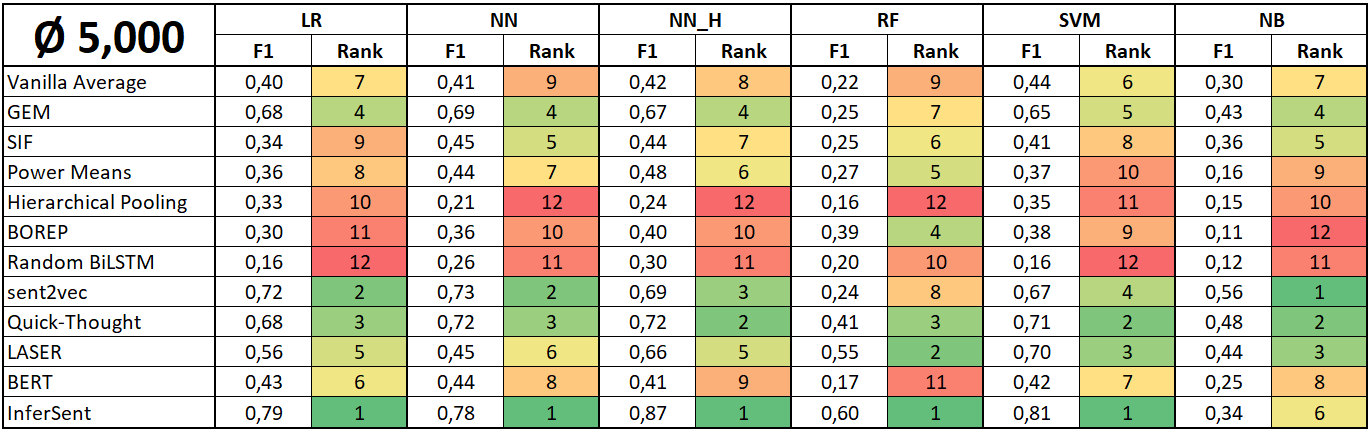
\includegraphics[scale=0.475]{images/results_wc_en_5000}
	\caption[Stability analysis results for 5k instances (\caps{WC} task, EN)]
		{Stability analysis results for 5k instances (\caps{WC} task, EN).}
\end{table}

\begin{table}[H]
	\centering
	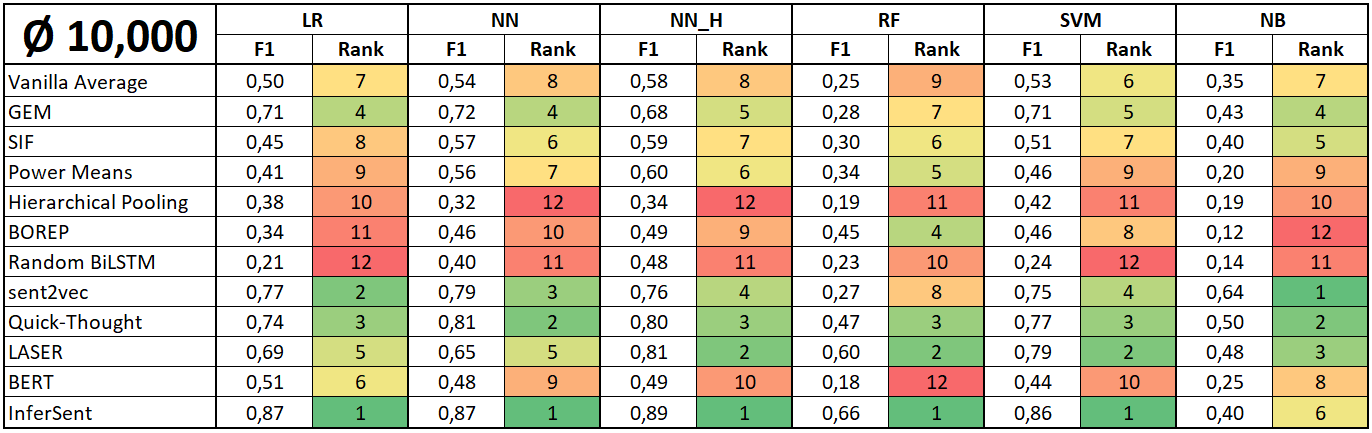
\includegraphics[scale=0.475]{images/results_wc_en_10000}
	\caption[Stability analysis results for 10k instances (\caps{WC} task, EN)]
		{Stability analysis results for 10k instances (\caps{WC} task, EN).}
\end{table}

\begin{table}[H]
	\centering
	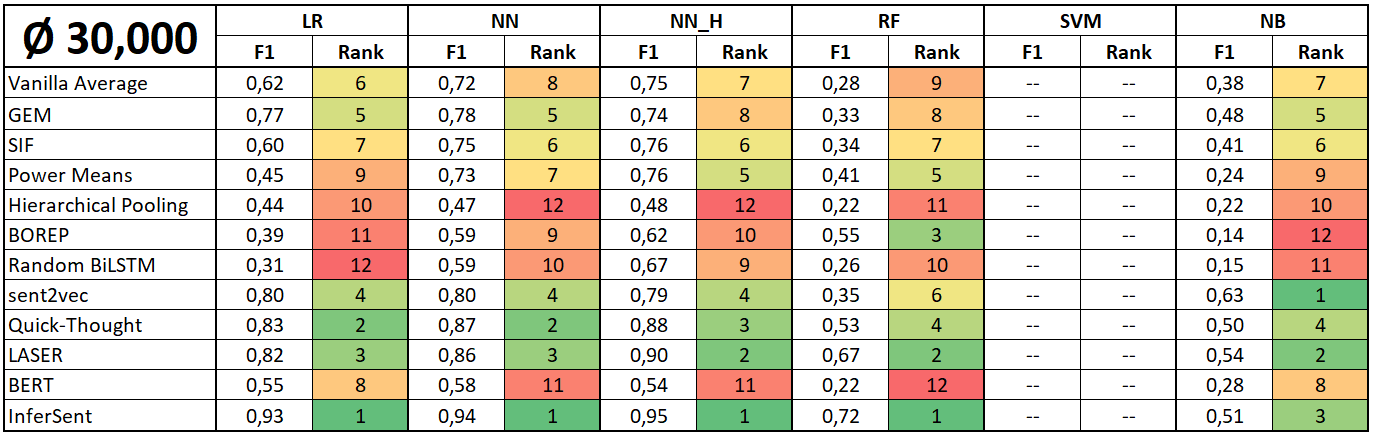
\includegraphics[scale=0.475]{images/results_wc_en_30000}
	\caption[Stability analysis results for 30k instances (\caps{WC} task, EN)]
		{Stability analysis results for 30k instances (\caps{WC} task, EN).}
\end{table}

\begin{table}[H]
	\centering
	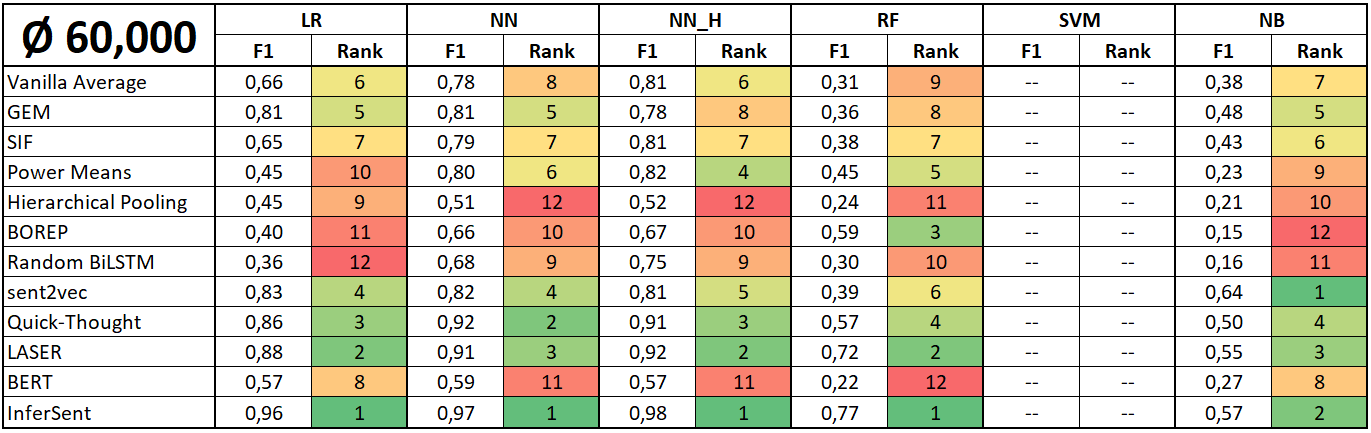
\includegraphics[scale=0.475]{images/results_wc_en_60000}
	\caption[Stability analysis results for 60k instances (\caps{WC} task, EN)]
		{Stability analysis results for 60k instances (\caps{WC} task, EN).}
\end{table}

\begin{figure}[H]
	\centering
	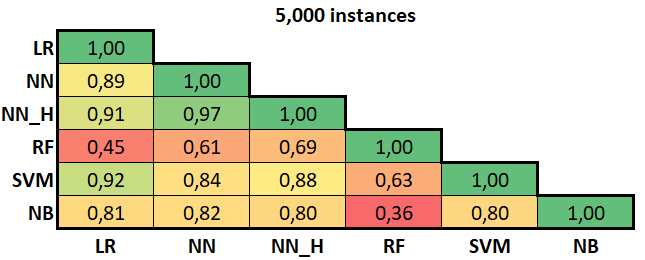
\includegraphics[scale=0.5]{images/corr_wc_en_5000}
	\caption[Classifier correlations with 5k instances (\caps{WC} task, EN)]
		{Classifier correlations with 5k instances (\caps{WC} task, EN).}
\end{figure}

\begin{figure}[H]
	\centering
	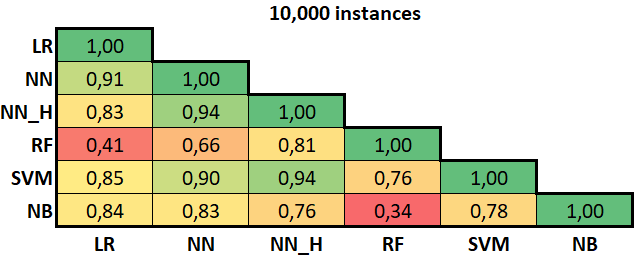
\includegraphics[scale=0.5]{images/corr_wc_en_10000}
	\caption[Classifier correlations with 10k instances (\caps{WC} task, EN)]
		{Classifier correlations with 10k instances (\caps{WC} task, EN).}
\end{figure}

\begin{figure}[H]
	\centering
	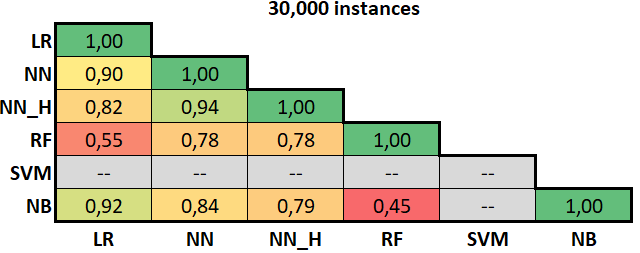
\includegraphics[scale=0.5]{images/corr_wc_en_30000}
	\caption[Classifier correlations with 30k instances (\caps{WC} task, EN)]
		{Classifier correlations with 30k instances (\caps{WC} task, EN).}
\end{figure}

\begin{figure}[H]
	\centering
	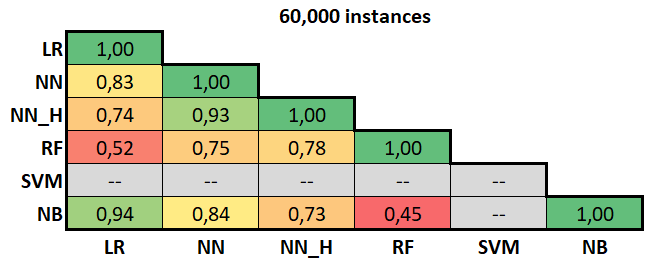
\includegraphics[scale=0.5]{images/corr_wc_en_60000}
	\caption[Classifier correlations with 60k instances (\caps{WC} task, EN)]
		{Classifier correlations with 60k instances (\caps{WC} task, EN).}
\end{figure}

% Table: Experiment results WC details deltas
\begin{table}[h]
	\centering
	\renewcommand{\arraystretch}{1.2}
	%\begin{adjustbox}{angle=90}
	\scalebox{0.9}{
	\begin{tabularx}{1.1\textwidth}{| X ? c | c | c ? c | c | c ? c | c | c ? c | c |}
		\hline
		\rowcolor{tud9c}
		\multicolumn{12}{| c |}{\textcolor{white}{\textbf{Absolute performance deltas in the \caps{WordContent} task
		(\texttt{NN\_H} classifier)}}}
		\\ \hline
		\rowcolor{tud9c!70}
													&
		\multicolumn{3}{ c ?}{
			\ding{182} $\bm{\Delta}$ \textbf{(im-)balance}} 
													&
		\multicolumn{3}{ c ?}{
			\ding{183} $\bm{\Delta}$ \textbf{(no) HP tuning}} 
													&
		\multicolumn{3}{ c ?}{
			\ding{184} $\bm{\Delta}$ \textbf{\texttt{NN} $\leftrightarrow$ \texttt{NN\_H}}}
													&
		\multicolumn{2}{ c |}{
			\ding{185} $\bm{\Delta}$ \textbf{size}}
		\\
		
		\rowcolor{tud9c!50}
		\multirow{-2}{*}{
			\cellcolor{tud9c!70}\textbf{Embedding}}	&
		\textbf{10k}		&
		\textbf{30k}		&
		\textbf{60k}		&
		\textbf{10k}		&
		\textbf{30k}		&
		\textbf{60k}		&
		\textbf{10k}		&
		\textbf{30k}		&
		\textbf{60k}		&
		\textbf{10k $\leftrightarrow$ 30k} &
		\textbf{30k $\leftrightarrow$ 60k}	
		\\ \hline\hline
		Vanilla average		& 0.21 & 0.13 & 0.09 & 0.05 & 0.01 &  0.00 & -0.04 	& -0.04 & 	-0.02 & 0.09 & 0.02
		\\ \hline
		p-Means 			& 0.20 & 0.12 & 0.09 & 0.02 & 0.00 &  0.00 & -0.03 	& -0.02 & 	-0.01 & 0.08 & 0.03
		\\ \hline
		SIF 				& 0.24 & 0.14 & 0.10 & 0.05 & 0.00 &  0.01 & -0.01 	& -0.02 & 	-0.01 & 0.07 & 0.01
		\\ \hline
		GEM 				& 0.17 & 0.12 & 0.09 & 0.03 & 0.04 &  0.04 &  0.01 	&  0.02 & 	 0.03 & 0.01 & 0.01
		\\ \hline
		hier. pooling 		& 0.29 & 0.23 & 0.22 & 0.03 & 0.01 &  0.00 & -0.04 	& -0.02 & 	-0.01 & 0.08 & 0.03
		\\ \hline
		BOREP			& 0.25 & 0.20 & 0.18 & 0.01 & 0.00 &  0.00 & -0.01	& -0.02 &	 0.00 & 0.08 & 0.03
		\\ \hline
		Random BiLSTM		& 0.23 & 0.17 & 0.14 & 0.05 & 0.00 &  0.00 & -0.08	& -0.07 &	-0.06 & 0.13 & 0.05
		\\ \hline
		InferSent 			& 0.07 & 0.03 & 0.01 & 0.01 & 0.00 &  0.00 & -0.02 	&  0.00 &  	 0.00 & 0.02 & 0.01
		\\ \hline
		Quick-Thought 		& 0.06 & 0.03 & 0.02 & 0.00 & 0.00 &  0.01 & -0.02 	&  0.00 &  	 0.00 & 0.05 & 0.02
		\\ \hline
		sent2vec 			& 0.22 & 0.20 & 0.18 & 0.01 & 0.00 &  0.00 &  0.00 	&  0.00 &  	 0.00 & 0.01 & 0.00
		\\ \hline
		BERT 			& 0.05 & 0.04 & 0.04 & 0.01 & 0.02 &  0.03 &  0.02 	&  0.03 &  	 0.02 & 0.04 & 0.03
		\\ \hline
		LASER 			& 0.09 & 0.03 & 0.02 & 0.02 & 0.01 &  0.00 & -0.08 	& -0.02 & 	-0.01 & 0.03 & 0.01
		\\ \hline
	\end{tabularx}}
	%\end{adjustbox}
	\caption[Absolute F1 performance deltas in the \caps{WC} task (\texttt{NN\_H})]
		{Absolute F1 performance deltas in the \caps{WC} task (\texttt{NN\_H}):
		\ding{182} Effect of \texttt{class balance} (positive number indicates positive effect of balanced data),
		\ding{183} Effect of \texttt{hyper-parameter tuning} (on balanced data),
		\ding{184} Effect of \texttt{classifier} (on balanced data; negative values indicate worse performance of \texttt{NN}) and
		\ding{185} effect of \texttt{size} (on balanced data sets).}
	\label{tab:wc_detail_deltas}
\end{table}

% Table: Experiment results WC Details with hp optimization
\begin{table}[h]
	\centering
	\renewcommand{\arraystretch}{1.2}
	\scalebox{0.9}{
	\begin{tabularx}{1.1\textwidth}{| X | r ? c | c | c | c ? c | c | c | c ? c | c | c | c |}
		\hline
		\rowcolor{tud9c}
		\multicolumn{14}{| c |}{\textcolor{white}{\textbf{Effect of hyper-parameter tuning in the \caps{WordContent} task
		(\texttt{NN\_H} classifier)}}}
		\\ \hline
		\rowcolor{tud9c!70}
													&
													&
		\multicolumn{4}{ c ?}{\textbf{10k}} 			&
		\multicolumn{4}{ c ?}{\textbf{30k}} 			&
		\multicolumn{4}{ c |}{\textbf{60k}}		
		\\
		
		\rowcolor{tud9c!50}
		\multirow{-2}{*}{
			\cellcolor{tud9c!70}\textbf{Embedding}}	&
		\multirow{-2}{*}{
			\cellcolor{tud9c!70}\textbf{Dim.}}			&
		\textbf{imbal.}								&
		\textbf{R}									&
		\textbf{bal.}									&
		\textbf{R}									&
		\textbf{imbal.}								&
		\textbf{R}									&
		\textbf{bal.}									&
		\textbf{R}									&
		\textbf{imbal.}								&
		\textbf{R}									&
		\textbf{bal.}									&
		\textbf{R}									
		\\ \hline\hline
%		\rowcolor{tud9c!30}
%		\multicolumn{14}{| c |}{\textbf{Neural net with hidden layer (\texttt{NN\_H}) \underl{and} hyper-parameter tuning}}
%		\\ \hline
		Vanilla average		& 300	& 0.70 & 8 	& 0.84 & 7  	& - & - & 0.89 & 7 	& - & - & 0.90 & 8 	
		\\ \hline
		p-Means			& 1,500	& 0.74 & 7 	& 0.82 & 8 	& - & - & 0.88 & 8 	& - & - & 0.91 & 6 	
		\\ \hline
		\gls{sif} 			& 300	& 0.79 & 6 	& 0.88 & 4 	& - & - & 0.90 & 5 	& - & - & 0.92 & 5 	
		\\ \hline
		\gls{gem} 			& 300 	& 0.84 & 4 	& 0.88 & 4 	& - & - & 0.90 & 5 	& - & - & 0.91 & 6 	
		\\ \hline
		hier. pooling		& 300	& 0.48 & 12 	& 0.66 & 11 	& - & - & 0.72 & 11 	& - & - & 0.74 & 11 	
		\\ \hline
		BOREP			& 4,096	& 0.53 & 11	& 0.75 & 10	& - & - & 0.82 &	 10	& - & - & 0.85 & 10
		\\ \hline
		Random BiLSTM		& 8,129	& 0.63 & 9		& 0.76 & 9		& - & - & 0.84 &	 9	& - & - & 0.89 & 9
		\\ \hline
		InferSent			& 4,096	& 0.93 & 1 	& 0.97 & 2 	& - & - & 0.98 & 2 	& - & - & 0.99 & 1 	
		\\ \hline
		Quick-Thought		& 2,400	& 0.87 & 3 	& 0.86 & 6 	& - & - & 0.91 & 4 	& - & - & 0.94 & 3 	
		\\ \hline
		sent2vec			& 700	& 0.80 & 5 	& 0.99 & 1 	& - & - & 0.99 & 1 	& - & - & 0.99 & 1 	
		\\ \hline
		BERT				& 768	& 0.55 & 10 	& 0.55 & 12 	& - & - & 0.60 & 12 	& - & - & 0.64 & 12 	
		\\ \hline
		LASER			& 1,024	& 0.90 & 2 	& 0.92 & 3 	& - & - & 0.94 & 3 	& - & - & 0.94 & 3 	
		\\ \hline
	\end{tabularx}}
	\caption[Effect of hyper-parameter tuning on the \caps{WC} probing task results (F1 scores)]
		{Effect of hyper-parameter tuning on the \caps{WC} probing task results (F1 scores). The results are
		reported for the \texttt{NN\_H} classifier.}
	\label{tab:wc_detail_hp_opt}
\end{table}

% Table: Experiment results WC details
\begin{table}[H]
	\centering
	\renewcommand{\arraystretch}{1.4}
	\scalebox{0.9}{
	\begin{tabularx}{1.1\textwidth}{| X | r ? c | c | c | c ? c | c | c | c ? c | c | c | c |}
		\hline
		\rowcolor{tud9c}
		\multicolumn{14}{| c |}{\textcolor{white}{\textbf{Effects of data set size and class balance in the
		\caps{WordContent} task}}}
		\\ \hline
		\rowcolor{tud9c!70}
													&
													&
		\multicolumn{4}{ c ?}{\textbf{10k}} 			&
		\multicolumn{4}{ c ?}{\textbf{30k}} 			&
		\multicolumn{4}{ c |}{\textbf{60k}}		
		\\
		
		\rowcolor{tud9c!50}
		\multirow{-2}{*}{
			\cellcolor{tud9c!70}\textbf{Embedding}}	&
		\multirow{-2}{*}{
			\cellcolor{tud9c!70}\textbf{Dim.}}			&
		\textbf{imbal.}								&
		\textbf{R}									&
		\textbf{bal.}									&
		\textbf{R}									&
		\textbf{imbal.}								&
		\textbf{R}									&
		\textbf{bal.}									&
		\textbf{R}									&
		\textbf{imbal.}								&
		\textbf{R}									&
		\textbf{bal.}									&
		\textbf{R}									
		\\ \hline\hline
		\rowcolor{tud9c!30}
		\multicolumn{14}{| c |}{\textbf{Neural network with hidden layer (\texttt{NN\_H})}}
		\\ \hline
		Vanilla average	& 300 	& 0.58 & 8 	& 0.79 & 8  	& 0.75 & 7 	& 0.88 & 6 	& 0.81 & 5 	& 0.90 & 7 	
		\\ \hline
		p-Means 		& 1,500 	& 0.60 & 6 	& 0.80 & 7  	& 0.76 & 5 	& 0.88 & 6 	& 0.82 & 4		& 0.91 & 5 	
		\\ \hline
		\gls{sif} 		& 300	& 0.59 & 7 	& 0.83 & 6  	& 0.76 & 5 	& 0.90 & 5 	& 0.81 & 5		& 0.91 & 5	
		\\ \hline
		\gls{gem} 		& 300 	& 0.68 & 5		& 0.85 & 5 	& 0.74 & 8 	& 0.86 & 8 	& 0.78 & 8		& 0.87 & 9 	
		\\ \hline
		hier. pooling	& 300	& 0.34 & 12 	& 0.63 & 11 	& 0.48 & 12 	& 0.71 & 11	& 0.52 & 12	& 0.74 & 11
		\\ \hline
		BOREP 		& 4,096	& 0.49 & 9		& 0.74 & 9		& 0.62 & 10	 & 0.82 & 10	& 0.67 & 10	& 0.85 & 10
		\\ \hline
		Random BiLSTM & 8,129	& 0.48 & 11	& 0.71 & 10	& 0.67 & 9		& 0.84 & 9		& 0.75 & 9		& 0.89 & 8
		\\ \hline
		InferSent		& 4,096	& 0.89 & 1		& 0.96 & 2		& 0.95 & 1 	& 0.98 & 2		& 0.98 & 1		& 0.99 & 1 	
		\\ \hline
		Quick-Thought	& 2,400	& 0.80 & 3		& 0.86 & 4		& 0.88 & 3 	& 0.91 & 4		& 0.91 & 3		& 0.93 & 4 	
		\\ \hline
		sent2vec		& 700	& 0.76 & 4 	& 0.98 & 1 	& 0.79 & 4 	& 0.99 & 1 	& 0.81 & 5		& 0.99 & 1	
		\\ \hline
		BERT			& 768	& 0.49 & 9 	& 0.54 & 12 	& 0.54 & 11 	& 0.58 & 12 	& 0.57 & 11	& 0.61 & 12	
		\\ \hline
		LASER		& 1,024	& 0.81 & 2 	& 0.90 & 3		& 0.90 & 2		& 0.93 & 3 	& 0.92 & 2		& 0.94 & 3	
		\\ \hline\hline
		\rowcolor{tud9c!30}
		\multicolumn{14}{| c |}{\textbf{Neural net without hidden layer (\texttt{NN})}}
		\\ \hline
		Vanilla average 		& 300 	& 0.54 & 8 	& 0.75 & 8 	& 0.72 & 8 	& 0.84 & 8		& 0.78 & 8 	& 0.88 & 8 	
		\\ \hline
		p-Means 			& 1,500 	& 0.56 & 7 	& 0.77 & 7		& 0.73 & 7 	& 0.86 & 7 	& 0.80 & 6 	& 0.90 & 5	
		\\ \hline
		\gls{sif} 			& 300	& 0.57 & 6		& 0.82 & 5		& 0.75 & 6 	& 0.88 & 5		& 0.79 & 7 	& 0.90 & 5	
		\\ \hline
		\gls{gem} 			& 300 	& 0.72 & 4		& 0.86 & 3 	& 0.78 & 5 	& 0.88 & 5		& 0.81 & 5 	& 0.90 & 5	
		\\ \hline
		hier. pooling		& 300	& 0.32 & 12	& 0.59 & 11	& 0.47 & 12	& 0.69 & 11	& 0.51 & 12 	& 0.73 & 11	
		\\ \hline
		BOREP 			& 4,096	& 0.46 & 10	& 0.73 & 9		& 0.59 & 9	 	& 0.80 & 9		& 0.66 & 10	& 0.85 & 9
		\\ \hline
		Random BiLSTM 	& 8,129	& 0.40 & 11	& 0.63 & 10	& 0.59 & 9		& 0.77 & 10	& 0.68 & 9		& 0.83 & 10
		\\ \hline
		InferSent			& 4,096	& 0.87 & 1		& 0.94 & 2		& 0.94 & 1 	& 0.98 & 2		& 0.97 & 1 	& 0.99 & 1 	
		\\ \hline
		Quick-Thought		& 2,400	& 0.81 & 2		& 0.84 & 4		& 0.87 & 2 	& 0.91 & 3 	& 0.92 & 2 	& 0.93 & 3
		\\ \hline
		sent2vec			& 700	& 0.79 & 3		& 0.98 & 1 	& 0.80 & 4 	& 0.99 & 1		& 0.82 & 4 	& 0.99 & 1	
		\\ \hline
		BERT				& 768	& 0.48 & 9		& 0.56 & 12	& 0.58 & 11 	& 0.61 & 12	& 0.59 & 11 	& 0.63 & 12	
		\\ \hline
		LASER			& 1,024	& 0.65 & 5		& 0.82 & 5		& 0.86 & 3		& 0.91 & 3		& 0.91 & 3		& 0.93 & 3	
		\\ \hline
	\end{tabularx}}
	\caption[Effects of class (im-)balance as well as data set size on the \caps{WC} probing task results (F1 scores)]
		{Effects of class (im-)balance as well as data set size on the results for the \caps{WC} probing task (F1 scores). The results are
		reported for the \texttt{NN\_H} classifier (top) as well as for the \texttt{NN} classifier (bottom).}
	\label{tab:wc_detail}
\end{table}

\newpage

% Georgian
% -----------------------------------------------------------------------------------------------------------------------------------------------------
\subsection{Georgian}

\begin{table}[H]
	\centering
	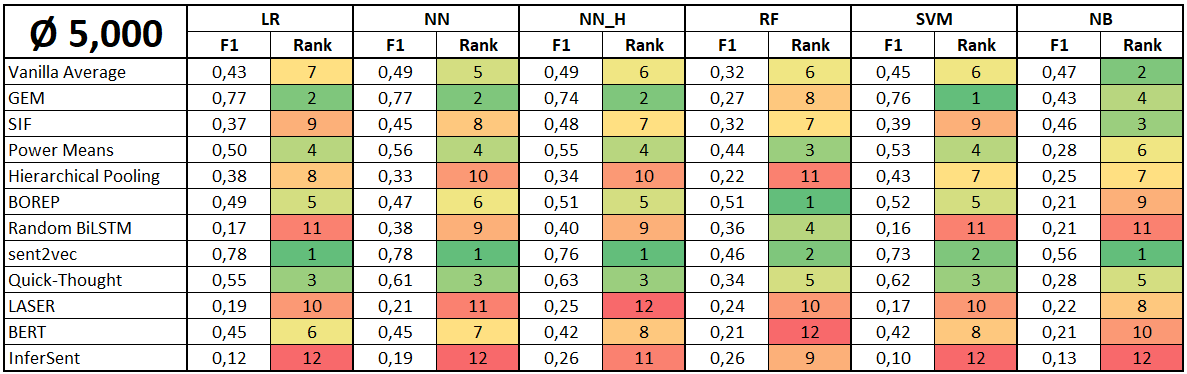
\includegraphics[scale=0.55]{images/results_wc_ka_5000}
	\caption[Stability analysis results for 5k instances (\caps{WC} task, KA)]
		{Stability analysis results for 5k instances (\caps{WC} task, KA).}
\end{table}

\begin{table}[H]
	\centering
	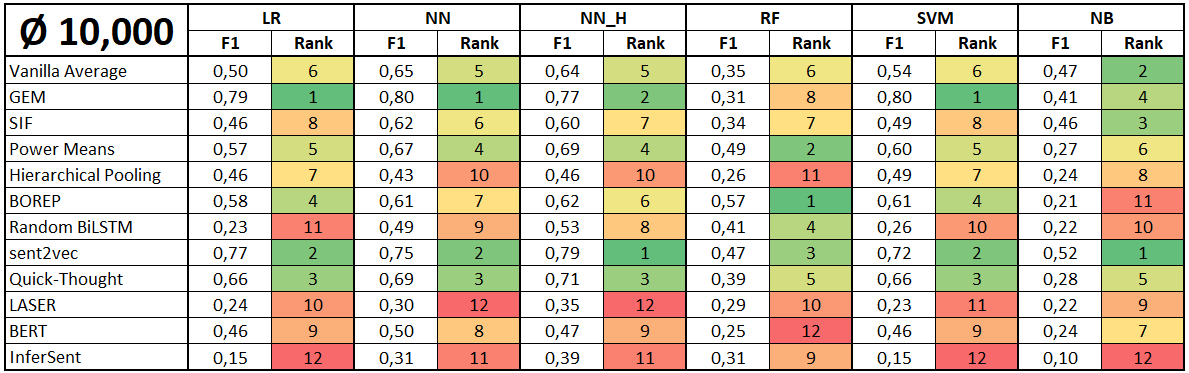
\includegraphics[scale=0.55]{images/results_wc_ka_10000}
	\caption[Stability analysis results for 10k instances (\caps{WC} task, KA)]
		{Stability analysis results for 10k instances (\caps{WC} task, KA).}
\end{table}

\begin{table}[H]
	\centering
	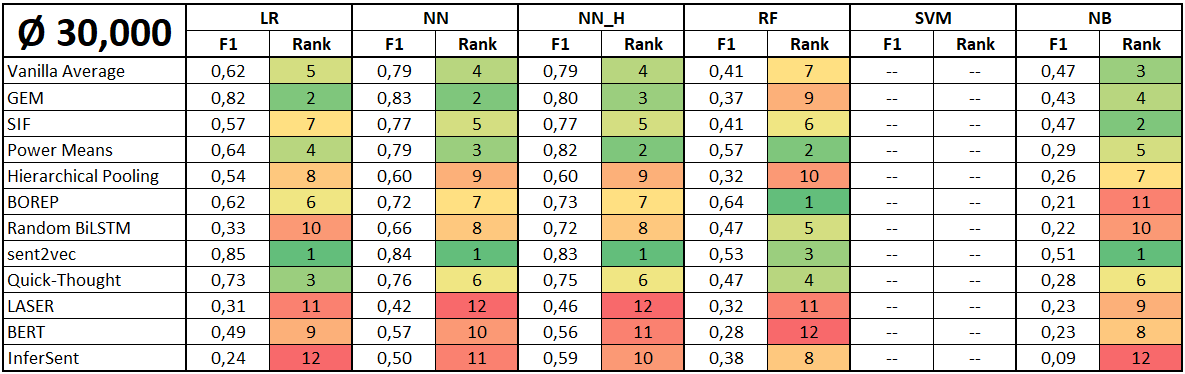
\includegraphics[scale=0.55]{images/results_wc_ka_30000}
	\caption[Stability analysis results for 30k instances (\caps{WC} task, KA)]
		{Stability analysis results for 30k instances (\caps{WC} task, KA).}
\end{table}

\begin{table}[H]
	\centering
	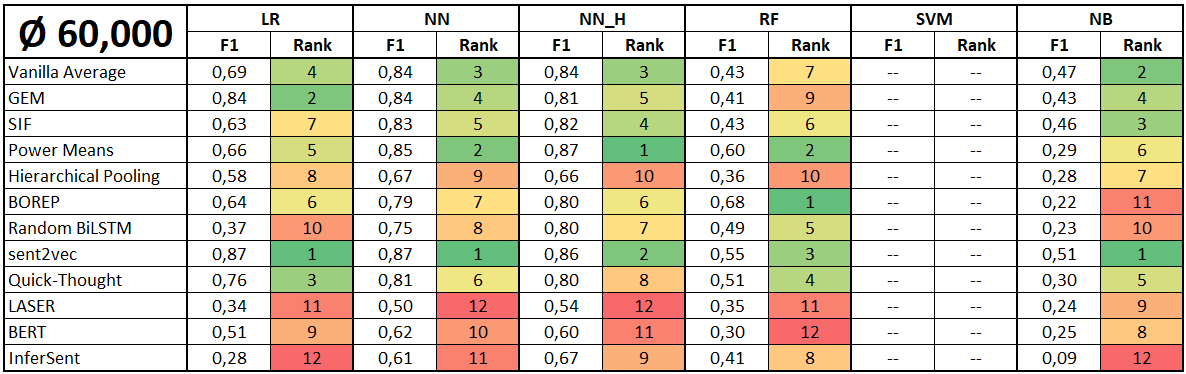
\includegraphics[scale=0.55]{images/results_wc_ka_60000}
	\caption[Stability analysis results for 60k instances (\caps{WC} task, KA)]
		{Stability analysis results for 60k instances (\caps{WC} task, KA).}
\end{table}

\begin{figure}[H]
	\centering
	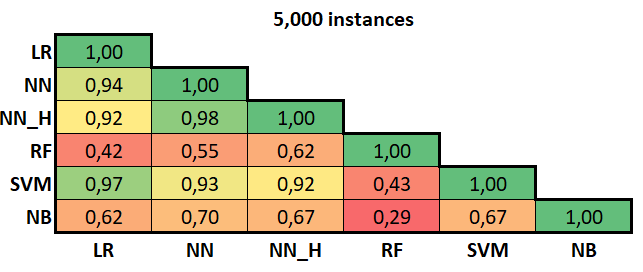
\includegraphics[scale=0.5]{images/corr_wc_ka_5000}
	\caption[Classifier correlations with 5k instances (\caps{WC} task, KA)]
		{Classifier correlations with 5k instances (\caps{WC} task, KA).}
\end{figure}

\begin{figure}[H]
	\centering
	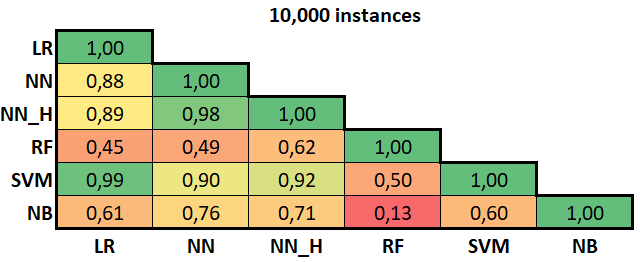
\includegraphics[scale=0.5]{images/corr_wc_ka_10000}
	\caption[Classifier correlations with 10k instances (\caps{WC} task, KA)]
		{Classifier correlations with 10k instances (\caps{WC} task, KA).}
\end{figure}

\begin{figure}[H]
	\centering
	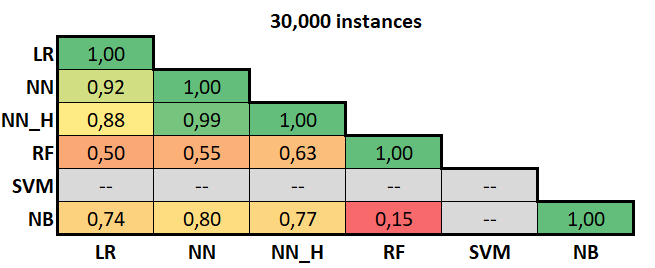
\includegraphics[scale=0.5]{images/corr_wc_ka_30000}
	\caption[Classifier correlations with 30k instances (\caps{WC} task, KA)]
		{Classifier correlations with 30k instances (\caps{WC} task, KA).}
\end{figure}

\begin{figure}[H]
	\centering
	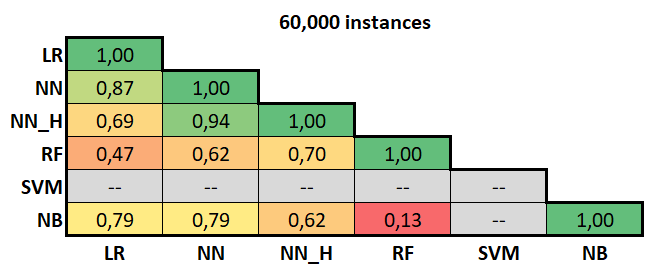
\includegraphics[scale=0.5]{images/corr_wc_ka_60000}
	\caption[Classifier correlations with 60k instances (\caps{WC} task, KA)]
		{Classifier correlations with 60k instances (\caps{WC} task, KA).}
\end{figure}

% Bibliography
% ------------------------------------------------------------------------------------

\newpage
\addcontentsline{toc}{section}{References}
\bibliography{bib/mybib}{}
\bibliographystyle{dwstyle}

\textbf{Webpages}

\url{https://1000mostcommonwords.com/} (retrieved: September 08, 2019) \\[2mm]
\url{https://achyutjoshi.github.io/aspect_extraction/aspectextraction} (retrieved: October 16, 2019) \\[2mm]
\url{https://blackboxnlp.github.io/} (retrieved: October 04, 2019) \\[2mm]
\url{https://cogcomp.seas.upenn.edu/page/resource_view/49} (retrieved: September 08, 2019) \\[2mm]
\url{https://www.colanguage.com/turkish-adjectives} (retrieved: October 02, 2019) \\[2mm]
\url{https://corpora.uni-hamburg.de/hzsk/de/islandora/object/treebank:hdt} (retrieved: September 07, 2019) \\[2mm]
\url{https://deacademic.com/dic.nsf/dewiki/510990} (retrieved: October 02, 2019) \\[2mm]
\url{https://dumps.wikimedia.org/} (retrieved: September 20, 2019) \\[2mm]
\url{https://emojipedia.org/} (retrieved: September 18, 2019) \\[2mm]
\url{http://gnc.gov.ge/gnc/page} (retrieved: September 07, 2019) \\[2mm]
\href{https://www.grammatiken.de/tuerkische-grammatik/tuerkisch-agglutinierende-sprache-suffix-anhaengen.php}{\texttt{https://www.grammatiken.de/tuerkische-grammatik/}} (retrieved: October 11, 2019) \\[2mm]
\url{http://ftp.gwdg.de/pub/ctan/fonts/georgian/mxedruli/mxeddoc.pdf} (retrieved: September 06, 2019) \\[2mm]
\href{https://www.ims.uni-stuttgart.de/forschung/ressourcen/korpora/tiger.html}{\texttt{https://www.ims.uni-stuttgart.de/}} (retrieved: September 07, 2019) \\[2mm]
\href{https://www.informatik.tu-darmstadt.de/ukp/research_6/data/argumentation_mining_1/ukp_sentential_argument_mining_corpus/index.en.jsp}{\texttt{https://www.informatik.tu-darmstadt.de/}} (retrieved: September 08, 2019)  \\[2mm]
\url{https://issuu.com/artemivantsov/docs/150_georgian_verbs} (retrieved: September 07, 2019) \\[2mm]
\url{http://jalammar.github.io/illustrated-bert/} (retrieved: September 04, 2019) \\[2mm]
\url{https://www.kaggle.com/crowdflower/twitter-airline-sentiment} (retrieved: September 08, 2019) \\[2mm]
\href{https://medium.com/pachyderm-data/hold-your-machine-learning-and-ai-models-accountable-de887177174c}{\texttt{https://medium.com/}} (retrieved: October 07, 2019) \\[2mm]
\url{https://www.mturk.com/} (retrieved: September 08, 2019) \\[2mm]
\href{https://www.russlandjournal.de/russische-literatur/gedichte-von-alexander-puschkin/}{\texttt{https://www.russlandjournal.de/}} (retrieved: September 06, 2019) \\[2mm]
\href{http://www.schule-mehrsprachig.at/fileadmin/schule_mehrsprachig/redaktion/sprachensteckbriefe/pdf/ssb_tuerkisch_neu.pdf}{\texttt{http://www.schule-mehrsprachig.at/}} (retrieved: September 06, 2019) \\[2mm]
\url{https://nlp.stanford.edu/projects/snli/} (retrieved: September 04, 2019) \\[2mm]
\href{https://towardsdatascience.com/the-black-box-metaphor-in-machine-learning-4e57a3a1d2b0}{\texttt{https://towardsdatascience.com/}} (retrieved: October 07, 2019) \\[2mm]
\url{http://ge.translit.cc/} (retrieved: September 07, 2019) \\[2mm]
\href{https://public.ukp.informatik.tu-darmstadt.de/arxiv2018-xling-sentence-embeddings/translated-snli/en-de-translated-snli-4x.zip}{\texttt{https://public.ukp.informatik.tu-darmstadt.de/}} (retrieved: September 04, 2019) \\[2mm]
\url{https://uni-tuebingen.de/de/134290} (retrieved: September 09, 2019) \\[2mm]
\url{https://universaldependencies.org/} (retrieved: September 07, 2019) \\[2mm]
\url{https://de.wikipedia.org/wiki/Georgische_Sprache} (retrieved: September 06, 2019) \\[2mm]
\url{https://en.wikipedia.org/wiki/Turkish_language} (retrieved: September 06, 2019) \\[2mm]
\url{http://www.wikiwand.com/fr/Arbre_syntaxique} (retrieved: September 05, 2019) \\[2mm]

\textbf{GitHub Repositories\github}

\url{https://github.com/attardi/wikiextractor} (retrieved: September 20, 2019) \\[2mm]
\url{https://github.com/epfml/sent2vec} (retrieved: September 04, 2019) \\[2mm]
\url{https://github.com/facebookresearch/InferSent} (retrieved: September 04, 2019) \\[2mm]
\url{https://github.com/facebookresearch/LASER} (retrieved: September 04, 2019) \\[2mm]
\url{https://github.com/facebookresearch/SentEval} (retrieved: September 03, 2019) \\[2mm]
\url{https://github.com/google-research/bert/blob/master/multilingual.md} (retrieved: September 04, 2019) \\[2mm]
\url{https://github.com/lajanugen/S2V} (retrieved: September 04, 2019) \\[2mm]
\url{https://github.com/tmikolov/word2vec} (retrieved: September 20, 2019) \\[2mm]
\url{https://github.com/UKPLab/arxiv2018-xling-sentence-embeddings} (retrieved: September 09, 2019)

\textbf{Videos}

\url{https://www.youtube.com/watch?v=ERibwqs9p38} (retrieved: September 03, 2019)

\textbf{Images}

\url{https://blog.f1000.com/wp-content/uploads/2017/06/black_box_blog.png} (retrieved: September 04, 2019)

\end{document}
